\documentclass[10pt,twoside]{memoir}

\usepackage{graphicx}
\usepackage[space]{grffile}
\usepackage{latexsym}
\usepackage{textcomp}
\usepackage{longtable}
\usepackage{multirow,booktabs}
\usepackage{amsfonts,amsmath,amssymb}
\usepackage{natbib}
\usepackage{url}
\usepackage{hyperref}
\hypersetup{colorlinks=false,pdfborder={0 0 0}}
% You can conditionalize code for latexml or normal latex using this.
\newif\iflatexml\latexmlfalse
\usepackage[utf8]{inputenc}
\usepackage[ngerman,english]{babel}

\date{June 2016}

\begin{document}

\author{JP Breuer\\ Affiliation not available  \and Awaiting Activation\\ Affiliation not available \and Awaiting Activation\\ Affiliation not available \and Aaron\\ Affiliation not available \and Yannis\\ Affiliation not available \and FruzsinaBacso\\ Affiliation not available \and Ricard\\ Affiliation not available \and Awaiting Activation\\ Affiliation not available \and Sridhar Remma\\ Affiliation not available \and Gustavo Feijóo\\ Affiliation not available \and Kristian Sloth Lauszus\\ Affiliation not available \and Johannes Linde\\ Affiliation not available \and Maja\\ Affiliation not available \and Agge Winther\\ Affiliation not available \and Paul Connetable\\ Affiliation not available \and Rasmus Lundby Pedersen\\ Affiliation not available}

\title{Spacecraft Instrumentation Europa Life Finder Mission}

\maketitle

\frontmatter

\autchapter{Abstract}{Kristian Sloth Lauszus}

This book was done as a compulsory assignment in the course Spacecraft Instrumentation Systems (30320) at National Space Institute at the Technical University of Denmark (DTU).\\

\noindent
The book will present a proposal for a mission to the Jovian moon Europa. The goal of the mission is to search for life forms in either the ice or the sub-surface water ocean that is believed to be present on the moon.

The relevant theory about the moon will first be discussed, then a strawman proposal will be presented. Details about the orbiter, communication system, lander, penetrator, and instrument suite will then be described. Each chapter will present the different challenges involved and present possible solutions to these. Each chapter will then come up with a design proposal and discuss its viability.


\tableofcontents

\mainmatter

\chapter{Introduction} % JP
% What is our purpose for the mission. Why? How will we achieve our mission objectives? Water, energy, nutrition
% Estimate:
% Mass, Volume, Power budgets
% Why are we going?
    % Are we alone?
    % Water, energy, nutritions
    % Use pasos

Throughout the billions of years of Earth geologic history,it still took several hundreds of millions of years before evolution allowed for complex, intelligent organisms to inhabit the Earth. As soon as free thinking and self-reflection was possible in animals, naturally some of the first questions were the big philosophical ones: What is the origin of life and the universe? What are the conditions necessary to support and develop life? Are we alone in the universe?

Despite advancements in technology,


\chapter{Problem Formulation}

\autsection{Orbiter}{Johannes Linde}
The Europa Reconnaissance Imaging System (ERIS) plays an important role in the first phases of the mission. During the early stages, the imaging system will be used to map the surface of Europa and provide the necessary data for selecting a suitable landing site for the lander and penetrator. At this point, it is expected to have one or more cameras on the orbiter, mapping the surface of Europa in both low and high resolution. The Imaging System will be located in the orbiter, performing its primary objectives during the early stages of the life finding mission mission and performing the secondary objectives after a successful landing on Europa.

\autsection{Landing}{Maja Tomicic}
The landing-module should be able to perform a soft pin-point landing on the desired landing spot. The landing procedure should be completely autonomous using real-time on-board data from relevant sensors that are carefully selected ensuring that they meet the requirements for the landing as well as being mass and power efficient. After landing, the primary goal is to get the payload out of the radiation environment, therefore the possibility of melting a preliminary hole in the ice and dropping the payload into it, is investigated.

%Feel free to expand on these
\section{Theory}
\autsubsection{Defining life}{Agge Winther}
How did life originate here on Earth, and can vi draw conclusions to life in other places of the Universe, especially on Europa and its oceans.

\autsubsection{Ice Characteristics}{Lukas Christensen}
To evaluate the viability of a landing and possibly penetrating mission to Europa, the characteristics of the moon's ice sheet should be investigated. This includes determining how heat is deposited in the moon and how this affects the ice layer. Additionally, the structural profile of the ice should be analyzed to see what it might tell about the nature of the ice and to find out if landing is realistic. Finally, the temperature profile of the ice should be determined in order to evaluate the viability of a penetrating, possibly thermal, probe.

\autsubsection{Convection}{Lukas Christensen}
The physics of convection should be investigated to ascertain if natural convection can be used as a means of water transportation within a penetrating thermal ice probe. Ideally, simulations should be performed to obtain quantitative measures of its viability.

\section{Orbiter}

%   Include in problem formulation
%   target 2p 
\autsection{Communications for Europa}{Gustavo Feijóo Carrillo}
%   Introductory paragraph
%   Mission Stages and necessary comm links
%       Interplanetary phase

%--> False ref handling
%\iffalse
%(seen on fig. \ref{fig:GalInst1} and \ref{fig:GalInst2})
%\fi
The perfect communication system for every situation in a space mission does not exist. Specific systems must be sized and designed to meet the requirements of every single mission phase and with the clear concept that no communications with the spacecraft equals the complete failure of the mission and, this mission poses an increased risk since more than one link will be needed after landing on Europa's surface and begins the descent to reach the sub-ice ocean.

A mission to Europa would be classified as an interplanetary mission, furthermore this one is much more than just that and requires careful considerations of the different scenarios that a mission for Europa's sub-ice ocean exploration requires. First, the interplanetary phase is considered from launch of the spacecraft until Jupiter's orbit insertion (JOI). Second, is the landing phase just after accomplishing EOI (Europa Orbit Insertion), where site determination and certification procedures are carried before the landing of the carrier itself. Third (and most importantly for this writing) is the penetrator release and its descent through the ice crust which requires new development for accomplishing a working communications link through several kilometers of ice. And, at this phase is where the main scientific objectives are to be carried out as well as the majority of all the mission's goals.

\begin{figure}[htb]
	\centering
	\includegraphics[width=\textwidth]{figures/comms/europaLinks}
	\caption{ \textit{DRAFT} Depiction of the three main stages of a mission to Europa from a telecommunications perspective.}
	\label{fig:europaLinks}
\end{figure}

The interplanetary link is feasible thanks to the development of deep space communication networks by ESA (ESTRACK) and NASA (DSN), increasing the reliability of communications and navigation of spacecrafts on missions beyond Earth's orbit. This makes the main hazard during this phase, the high radiation environment of interplanetary space which requires designing for single fault tolerance, a redundant transponder system would be the must straight forward approach. Other problem for this mission stage is the pointing of the antennas since the higher gains needed, increase the requirements for the attitude control systems to keep direct line of sight with ground tracking stations. Universal Space Transponders (UST) are available for down/up-link in X-band and Ka-band down-link (X,Ka-band is TRL-4 according to \cite{clipper}). This leads to focus on the details of a link with a possible Europa orbiter as relay station, and more important the communications through the ice crust between the penetrator and the lander. Another critical component is autonomous operations, the most critical communication situation is for landing site determination and landing maneuvers as the propagation delay of 1 hour and 46 minutes makes only an autonomous solution possible which will need the highest data link coherence, robustness and concurrency implemented through Telecommand and Data Handling protocols.

The problem of establishing communications between the penetrator and the lander for command and telemetry as well as scientific data download is the propagation medium. The Europan ice crust is yet to be fully characterized, most models rely on data from 2 to 4 flybys from the Galileo mission and have developed models for the crust behaviour and composition as found in \cite{Chyba}. The ice losses aren't an issue itself since it has been well established through empirical work and modeling, as found in \cite{iceLink-scott}. Liquid water is considered opaque at radio- and micro-wave frequencies but in frozen state, water ice shows a very low imaginary dielectric constant which dictates the level of intensity loss of an electromagnetic plane wave traveling through this medium, this constant $\epsilon''$ is about a thousand times smaller than for liquid water. This fact allows for the possibility of an ice based communications link. In the following chapters a more detailed section on how the ice losses are expected to be found at Europa will be exposed. This detailed section will include a discussion on the effect of salt contents in the ice and its effect on the propagation loss. Similarly, the effect of different ice temperature must be discussed since it has a major contribution on the propagation loss of this medium. A link able to cope with this propagation losses is what will allow the penetrator to melt through several kilometers of ice and complete the mission objectives following the ice crust depth at the landing site is considered unknown, spanning from a few thousand meters $(2-4 km)$ to a thick crust close to $(10-20 km)$ wide.

Other problem for the penetrator-lander link is the the liquid water and "slushy" ice surrounding the penetrator vessel, a good understanding of the melt-refreeze cycle must be reached in order to achieve a robust communications link. Previous studies carried out by JPL for a similar mission concept requiring a through-ice link assumed the refreezing without providing further detail \cite{iceLink-scott}, for this mission this assumption is not good enough and must seek deeper understanding as stated before. 

\begin{figure}[htb]
	\centering
	\includegraphics[width=\textwidth]{figures/comms/meltColCycle_0}
	\caption{ \textit{DRAFT} Depiction of the plausible melted water column forming behind the penetrator with possible adverse effect on the performance of the communications from penetrator to lander. This column could be as short as 4 m or reach a few tens of meters.}
	\label{fig:meltColumn_broad}
\end{figure}


\autsection{Lander}{Maja Tomicic}
The landing-module should be able to perform a soft pin-point landing on the desired landing spot. The landing procedure should be completely autonomous using real-time on-board data from relevant sensors that are carefully selected ensuring that they meet the requirements for the landing as well as being mass and power efficient. After landing, the primary goal is to get the payload out of the radiation environment, therefore the possibility of melting a preliminary hole in the ice and dropping the payload into it, is investigated.

\section{Penetrator}
\autsubsection{Drilling Methods}{Lukas Christensen}
In order to get through the ice sheet on Europa some sort of penetration method is needed. Various possible solutions must be identified, and each must be analyzed to determine its viability. Once a method has been selected it must be thoroughly investigated and estimates for the penetration time must be provided and validated as it will form the basis of the overall mission design.

\autsubsection{Instrument Suite}{Morten Lykke Hilligsøe}
The instrument suites purpose is to generate data from which the following questions (presented in prioritized order) can be answered:
\begin{enumerate}
    \item Does life currently exist on Europa?
    \item Has life previously existed on Europa?
    \item How well are the conditions of Europa suited for life?
    \item What are the general characteristics of Europa?
\end{enumerate}

The presented questions will obviously rely on our definition of life, but if extraterrestrial life is anything like on earth, indicators will include the basic building blocks of life, chemical requirements and products of life such as trace metals and gasses, complex biochemical molecules which won’t be synthesized by simple physical processes and various physical requirements such as energy and temperature. The situation therefore requires several instruments to analyze the chemical, biochemical and physical composition, as well as a system for sample extraction and handling.

The problem definition at hand is then to make sure that if any form of life is present, the instrument suite will deliver the best possible data for detection and registration of this life. This kind of detection and analysis is constantly performed on earth, but a space mission to the subsurface sea of Europa places hard restrictions on the weight, volume, power consumption, durability and autonomy of such instruments. Therefore the optimal combination of instruments must be found, which support each other in the detection of life, while simultaneously complying with the restrictions at hand. 

As the surface of Europa presents an extremely hostile environment of vacuum, low temperatures and high radiation levels, answers to the questions presented are only sought after below the icy surface. Not only because life is not expected to be observed at the surface, but also because this will impose huge restrictions on the type of equipment capable of surviving these conditions, as well as added complexity, weight and costs. Instead the instruments will be protected by the lander and penetrator until safely inside the European ice crust.



%\section{Mission Layout}

%\input{gfc/prob-MissionLayout}

%This list is nothing right?...
%1. Mission Stages from a communications standpoint
 %   1.1 Journey to Jovian System
 %   1.2 Descent Maneuver
 %   1.3 Through-ice communications
 %   1.4 Science Phase Data Relay
%2. General Drivers
%3. Assumptions and Models for Europa Communications

%\section{Problem Limitation}


\chapter{Theory}

In this chapter some of the different theories about the moon will be presented. This includes some of the general theories moon about the environment and its characteristics. The theory and some simple calculations about the ice structure and temperature will then be discussed. The definition of life itself will be evaluated and finally the needed descent profile of the lander will be introduced.

\section{Moon Characteristics} % JP, Yannis

% General info: https://en.wikipedia.org/wiki/Colonization_of_Europa

\iffalse
* Rock core, water, ice

    * Why do we think so?
    
    * Geysers?
\fi 

%\subsection{Radiation Environment} \label{chap:radiation}%  "landing site guys", "orbiter guys"
%* Both for the orbiter and the lander
%Radiation: http://zimmer.csufresno.edu/~fringwal/w08a.jup.txt

\autsubsection{Tidal Wave}{Kristian Sloth Lauszus and Lukas Christensen}

\section{Ice characteristics}
In this section the different theories about the ice characteristics will be presented. This includes the structural profile and a simplified calculation of the ice temperature profile. Furthermore the concept of water convection will be presented, as it might eliminate the needs for low-pressure pump system to circulate the water into the different instruments.

\autsubsection{Structural Profile}{Rasmus Lundby Pedersen}\label{sec:structural_profile}

The first space probe flybys took place in the early 1970s, and Europa quickly became one of the main focuses in the search for past or present extraterrestrial life-harbouring environments, within reachable distances. Already in the 1960's were it discovered from earth-based observations, that the surface of Europa was covered in solid ice, not much unlike other satellites located that deep in the cold reaches of our solar-system. However, data recovered from satellite flybys supplied us with new information about the geology and composition of the moon's surface, having since helped us understanding the of Jupiter's, arguably, most interesting moons with respect to life-supporting environments.\\
\\
The Voayger mission from the late 1970's sent back coarse imagery of Europa with resolution in the ranges of kilometres per pixel, carrying valuable information about the surface of the Jovian satellite\cite{VoyagImg}. More specifically, the images showed a surface resembling that of a ball of string, discarding theories of Europa having a smooth surface, with it in stead being full of bands and ridges.\\%See requested article from DTU Findit
The Galileo spacecraft was launched in 1989 and entered orbit around Jupiter in 1995. It started transmitting data back to earth, from its extensive remote-sensing instrument suite
\iffalse 
(seen on fig. \ref{fig:GalInst1} and \ref{fig:GalInst2})
\fi
 with resolution surpassing Voayger's images almost three orders of magnitude. 
\iffalse
\begin{figure}[htb]
	\centering
	\includegraphics[width=\textwidth]{figures/Rasmus/GalileoInstrument1}
	\caption{Instrument suite of the 1989 Galileo mission.\cite{SciStrat} (\textit{Continued in fig. \ref{fig:GalInst2}}). \label{fig:GalInst1}}
\end{figure}
\begin{figure}[htb]
	\centering
	\includegraphics[width=\textwidth]{figures/Rasmus/GalileoInstrument2}
	\caption{Instrument suite of the 1989 Galileo mission.(Continued from fig. \ref{fig:GalInst1}) \cite{SciStrat} .\label{fig:GalInst2}}
\end{figure}
\fi
\\
The high-resolution measurements showed what seemed to be blocks of ice filled with ridges and/or early cracks, that had been lifted and rotated at some point in time. These disruptions indicates that there might be a liquid or softer slushy layer underneath the solid ice surface that through movement had broken and relocated the ice-crust. These cracks are illustrated on fig. \ref{fig:SurfCrack}, which is one picture of a series from the 1989 Galileo satellite\cite{HidOcean}. In any case, it indicates that there is some kind of structural activity in the outermost layer of the moon.\\
\\

\begin{figure}[htb]
	\centering
	\includegraphics[width=\textwidth]{figures/Rasmus/SurfCrack}
	\caption{Image of Europa's surface taken by the Galileo satellite, showing ridges and disruptions in the surface. \label{fig:SurfCrack}\cite{HidOcean}}
\end{figure}

% Surface Composition
As explained in the study made by the Space Studies Board's Committee on Planetary and Lunar Exploration (COMPLEX), the data from Galileo’s Near-Infrared Mapping Spectrometer (NIMS) show that the water-ice absorption of Europa doesn't match with the expected outcome of pure-water ice, even for areas where the level of frozen sulfur oxide is thought to be lowest (The source of this $SO_2$ is presumably volcanic eruption on Io.). There has been some theories on the cause of this, including the presence of salts and other minerals in the ice but recent studies show that bubbles and fractions could result in the same discrepancies and band shifts in the measurements. However, it is still believed that some of the darker spots seen on the moon are observed because of salts and minerals like hexahedrite, epsomite, and natron\cite{SciStrat}. % INDSÆT The identity of that contaminant so far eludes scientists, but sulfur or iron compounds are suspected from Hidden Ocean P. 8
\\
\\
The actual thickness of the theorized ice-crust, and even the complete structural model of the moon, is still subject to many discussions. It was previously (prior to the Galileo mission) believed that the moon could be consisting of a hydrated silicate core coated in a thin layer of water-ice. However, with the measurements of Europa's gravitational field done by the Galileo satellite has this theory since been largely debunked. The current popular belief is that the cores is either a solid or fluid metallic core surrounded by a layer of water and ice of more than 100km due to the estimated density of the Jovian body. \\
The global ratio between liquid and solid water-ice is still unknown since it must be based on assumptions about the internal structure of the ice, which in themselves are extremely uncertain. The estimates we do have are even based on local imagery, since making them on a global basis requires dedicated orbiter mission, like the planned CLIPPER mission.\\%INDSÆT REFERENCE
In one study, the impact craters of Europa are analysed and compared with computer simulations to estimate regional crust thickness. The rationale is, that central peaks found in craters on the surface resemble material uplift caused by meteor impacts on extraterrestrial planets\cite{ThickImpact}, as seen on fig. \ref{fig:ImpactPic}. Therefore, it is assumed that the crust is thick enough to prevent complete surface penetration from meteor impact and as such they conclude that the ice at the impact sites must have been more than 	$\mathbf{3-4km}$ thick. Graphical representation of the simulation results can be seen on fig. \ref{fig:ImpactSim}. Another study that also investigated the impact craters, and taken from their introduction: "Stereo topographic profiles suggest that the plateau [a plateau SW of Cilix impact crater] is
flexurally supported, with an effective elastic thickness $t_e$ of
$~6km$. For a conductive temperature profile this $t_e$ value
implies a solid ice shell thickness of $\mathbf{~15km}$; if the shell is
convecting, this estimate is a lower bound. Combined with
independent estimates, we infer a probable shell thickness
of $\mathbf{25 km}$. The shell thickness is likely to be uniform over
the entire satellite."\cite{ThermElast}
\begin{figure}[htb]
	\centering
	\includegraphics[width=\textwidth]{figures/Rasmus/Impacts}
	\caption{Galileo images of Europan central peak craters. (\textbf{A}) Brigid ($11^\circ$N, $80^\circ$W), $D=8.5km$. (\textbf{B}) Grainne ($60^\circ$S, $95^\circ$W), $D=13.5$km. (\textbf{C}) Cilix ($2.6^\circ$N, $182^\circ$W ), $D18.4$km. (\textbf{D}) Amergin ($14^\circ$S, $230^\circ$W), $D=18.6$km. (\textbf{E}) Maeve ($58^\circ$N, $75^\circ$W ), $D=20.4$km. (\textbf{F}) Pwyll ($25^\circ$S, $271^\circ$W), $D=23.7$ km. All images are at a resolution of 250 m/pixel and each is illuminated from the right except Cilix (\textbf{C}), which was observed at high sun
	\cite{ThickImpact}. D is crater diameter. \label{fig:ImpactPic}}
\end{figure}
\begin{figure}[htb]
	\centering
	\includegraphics[width=1\textwidth]{figures/Rasmus/Impacts2}
	\caption{Model results for impacts of large (A through C) and small projectiles (D through F) into 9-km-thick ice (gray) over liquid water (A) and (D), 5-kmthick ice (gray) over liquid water (black) (B) and (E), and 3-kmthick conductive lid (light gray) over convecting ice (dark gray) (C) and (F). Solid, dotted, and dashed lines show the regions of complete vaporization, complete melting, and $50\%$ melting, respectively.
	\cite{ThickImpact}.\label{fig:ImpactSim}}
\end{figure}
\\
Thermal models has also been used to estimate the average ice shell thickness of Europa. One study is carried out with the assumption of a ice shell decoupled from a silicate core by a layer of liquid water \cite{ThermThick}, so its conclusion may not fit with modern theories. They estimate the shell to have a thickness of $\mathbf{13-25km}$, depending on which thermal rheology model is used (Maxwell and general flow rheology, with and without heat flow from the core). Another thermal model is based on the suggestios of Europa having a metallic core and a silicate mantle, covered by significant layer of liquid water and a thinner ice shell \cite{ThermThick2}. The study heavily relies on convection in the ice, and this complicates the study further. The heat flow through the ice is dependant on the shell thickness, and shell thickness is in turn dependant on the heat flow. This study concludes on the result that the average thickness of a completely frozen shell must be around $\mathbf{36km}$ based on the study's assumptions.
\\
\\ One study carried out by [J.M. Wahr, M.T. Zuber et al., 2006] analyses the tidal effects caused by the differentiating gravitational pull from Jupiter, as Europa travels in its elliptical orbit around the planet. The result of the study is a set of analytical equations estimating the global thickness based on the Love-number of Europa. However, in order to utilize these equations, accurate knowledge of the ice-composition is required, as well as precise estimates of the Love numbers. In the end they even conclude conclude that their results may not be sufficient since they only provide an accuracy of $\pm 5\mathrm{km}$.\\
\\
Apart from the thickness and elemental composition of the ice, internal structure in the shelf is also highly relevant to the planned penetrator mission. Assuming a completely homogeneous ice-shelf is a crude over-simplification and may be a mission-killer if alternatives aren't considered. 
\begin{figure}[htb]
	\centering
	\includegraphics[width=0.5\textwidth]{figures/Rasmus/ArtLake}
	\caption{Artistic illustration of potential water lense, or lake, in the ice shell. \label{fig: ArtLake}}
\end{figure}
As such, apparent "Chaos Regions" has been observed on the surface of Europa and their causes has for a long time alluded scientists. However, recent studies suggests that these are formed due to water lenses in the shell, which can also be interpreted as lakes of liquid water \cite{IceLakes}. They way even be present within $3km$ of the surface, and it is estimated that there may be a water lense consisting of $20,000 - 60,000km^3$ of liquid water beneath the so-called Thera Macula chaos region. An artistic illustration of this phenomenon is shown on fig \ref{fig: ArtLake}.

\iffalse
* Ice thickness

* Composition of the ice? % Se: SWRI: "barr-showman-2009" (ask Kristian Lauszus)

* Lakes?
\fi

\autsubsection{Ice temperature profile}{Kristian Sloth Lauszus}
\label{sec:IceTemperatureProfile}

%* Indirect: salinity, melting speed
%* Drill sample
%* Passive screw in the tip
%	* Thermal isolated
%* Measure heat conductivity of the water
%	* Can be used to estimate the salinity of the water
%		* Melting speed
%
%* "back of the envelope" calculations

In order to estimate the descent time it is important to know the ice temperature profile i.e. the temperature change as a function of the depth and the energy required in order to melt the column of ice. The thermal conductivity of polycrystalline ice can be calculated according to the following equation\cite[(2.3)]{article:thermalConductivity}:
\begin{equation}
	k(T) = \frac{a_1}{T} + a_0
\end{equation}
Where the constants $a_1$ and $a_0$ are given by:
\begin{align}
	a_1 &= \unitfrac[4.88 \e7]{ergs}{cm \, s} \\ \nonumber
		&= \unitfrac[488]{W}{m} \\
	a_0 &= \unitfrac[4.68 \e4]{ergs}{cm \, K \, s} \\ \nonumber
		&= \unitfrac[0.468]{W}{m \, K}
\end{align}
The boundary conditions for the temperature is simply given by 273.15 K at the transition between the water and ice and 100 K at the surface of the moon\cite{article:thermalConductivity}. Thus the temperature difference can be calculated:
\begin{align}
	& T_m = \unit[273.15]{K} \\
	& T_s = \unit[100]{K} \\
	& T_\Delta = T_m - T_s = \unit[173.15]{K}
\end{align}
Figure \ref{fig:T_vs_k} shows two plots of the thermal conductivity as a function of the temperature. Figure \ref{fig:T_vs_k_full} shows the thermal conductivity from 0 K to 273.15 K, figure \ref{fig:T_vs_k_zoom} on the other hand shows only shows the thermal conductivity in the range of the boundary conditions.
\begin{figure}[htb]
	\centering
	\subfloat[From 0 K to 273.15 K]{
		\includegraphics[width=.48\textwidth]{figures/temperature/T_vs_k}
		\label{fig:T_vs_k_full}
	}
	\subfloat[From $T_s$ to $T_m$]{
		\includegraphics[width=.48\textwidth]{figures/temperature/T_vs_k_zoom}
		\label{fig:T_vs_k_zoom}
	}
	\caption{Thermal conductivity as a function of the temperature}
	\label{fig:T_vs_k}
\end{figure}
The conductive heat transfer can be calculated fairly easily using Fourier's Law\cite{website:conductiveHeatTransfer}:
\begin{align}
	q(T) &= \frac{k(T) A T_\Delta}{d}
\end{align}
The area $A$ is the area of the penetrator facing the ice and by assuming a cylinder with a radius of 10 cm the area is given by:
\begin{align}
	A &= \pi \, 0.1^2 \approx \unit[0.03]{m^2}
\end{align}
Figure \ref{fig:T_vs_q} shows a plot of the conductive heat transfer as a function of the temperature. The thickness of the ice $d$ is assumed to be 3 km according to chapter \ref{sec:structural_profile}.
\begin{figure}[htb]
	\centering
	\includegraphics[width=.48\textwidth]{figures/temperature/T_vs_q}
	\caption{Conductive heat transfer as a function of the temperature}
	\label{fig:T_vs_q}
\end{figure}
Notice how both the conductive heat transfer $q$ and the thermal conductivity $k$ are approximately constant doing the interval $T_s$ to $T_m$, thus they can both be approximated by the average over the interval:
\begin{align}
	\bar{k} &= \unitfrac[3.80]{W}{m \, K} \\
	\bar{q} &= \unit[0.0066]{W}
\end{align}
Now the temperature as a function of the depth $d$ can be calculated assuming that the heat transfer and thermal conductivity are constant throughout the ice:
\begin{align}\label{eq:T_d}
	T(d) &= T_s + d \frac{\bar{q}}{\bar{k} A} = 100 K + \unitfrac[0.058 d]{K}{m}
\end{align}
Figure \ref{fig:d_vs_T} shows a plot of the temperature as a function of the depth into the ice.
\begin{figure}[htb]
	\centering
	\includegraphics[width=.48\textwidth]{figures/temperature/d_vs_T}
	\caption{Temperature as a function of the depth}
	\label{fig:d_vs_T}
\end{figure}
Figure \ref{fig:T_vs_rho} shows the density of ice as a function of the temperature using the values found in Table \ref{tab:ice_density}. This is be approximated by a linear second order function:
\begin{equation}\label{eq:rho_approx}
	\rho(T) = 931.21 - 0.68 \e{-3} T - 0.19 \e{-3} T^2
\end{equation}
Figure \ref{fig:T_vs_rho_approx} shows a plot of the approximated density of ice as a function of the temperature.
\begin{figure}[htb]
	\centering
	\subfloat[Density of ice according to Table \ref{tab:ice_density}]{
		\includegraphics[width=.48\textwidth]{figures/temperature/T_vs_rho}
		\label{fig:T_vs_rho}
	}
	\subfloat[Approximated ice density using \eqref{eq:rho_approx}]{
		\includegraphics[width=.48\textwidth]{figures/temperature/T_vs_rho_approx}
		\label{fig:T_vs_rho_approx}
	}
	\caption{Density of ice as a function of the temperature}
\end{figure}
\begin{table}[htb]
	\centering
	\resizebox{\textwidth}{!}{%
	\begin{tabular}{|c|c|c|c|c|c|c|c|c|c|c|c|c|c|c|c|}\hline
		$\mathbf{T} ~ (K)$ & 273.15 & 268.15 & 263.15 & 258.15 & 253.15 & 248.15 & 243.15 & 238.15 & 233.15 & 223.15 & 213.15 & 203.15 & 193.15 & 183.15 & 173.15 \\ \hline
		$\mathbf{\rho} ~ (\unitfrac{kg}{m^3})$ & 916.2 & 917.5 & 918.9 & 919.4 & 919.4 & 919.6 & 920.0 & 920.4 & 920.8 & 921.6 & 922.4 & 923.3 & 924.1 & 924.9 & 925.7 \\ \hline
	\end{tabular}}
	\caption{Density of ice for different temperatures\cite{website:iceDensity}}
	\label{tab:ice_density}
\end{table}
Now the density as a function of the distance can be calculated by inserting \eqref{eq:T_d} into \eqref{eq:rho_approx}:
\begin{equation}\label{eq:rho_approx_d}
	\rho(d) = 929.29 - 0.22 \e{-2} d - 6.19 \e{-7} d^2
\end{equation}
%A plot of \eqref{eq:rho_approx_d} and \eqref{eq:T_diff} can be seen in Figure \ref{fig:d_vs_rho} and Figure \ref{fig:d_vs_T_delta} respectively.
%\begin{figure}[htb]
%	\centering
%	\captionsetup[subfigure]{width=0.45\textwidth}
%	\subfloat[Ice density as a function of the depth using \eqref{eq:rho_approx_d}]{
%		\includegraphics[width=.48\textwidth]{figures/temperature/d_vs_rho}
%		\label{fig:d_vs_rho}
%	}
%	\subfloat[Temperature difference as a function of the depth]{
%		\includegraphics[width=.48\textwidth]{figures/temperature/d_vs_T_delta}
%		\label{fig:d_vs_T_delta}
%	}
%	\caption{}
%\end{figure}
Figure \ref{fig:T_vs_Cice} shows the specific heat capacity of ice plotted using the data found in Table \ref{tab:ice_heat_capacity}. Again this is approximated using a linear second order function:
\begin{equation}\label{eq:Cice_approx}
	C_{ice}(T) = -372.95 + 12.34 T - 0.013 T^2
\end{equation}
The specific heat capacity of ice as a function of the distance can be calculated by inserting \eqref{eq:T_d} into \eqref{eq:Cice_approx}:
\begin{equation}\label{eq:Cice_approx_d}
	C_{ice}(d) = 734.76 + 0.57 d - 0.42 \e{-4} d^2
\end{equation}
A plot of the approximated specific heat capacity can be seen in Figure \ref{fig:T_vs_Cice_approx}.
\begin{figure}[htb]
	\centering
	\subfloat[Specific heat capacity of ice according to Table \ref{tab:ice_heat_capacity}]{
		\includegraphics[width=.48\textwidth]{figures/temperature/T_vs_Cice}
		\label{fig:T_vs_Cice}
	}
	\subfloat[Approximated specific heat capacity of ice using \eqref{eq:Cice_approx}]{
		\includegraphics[width=.48\textwidth]{figures/temperature/T_vs_Cice_approx}
		\label{fig:T_vs_Cice_approx}
	}
	\caption{Specific heat capacity of ice as a function of the temperature}
\end{figure}
\begin{table}[htb]
	\centering
	\resizebox{\textwidth}{!}{%
	\begin{tabular}{|c|c|c|c|c|c|c|c|c|c|c|c|c|c|c|c|}\hline
		$\mathbf{T} ~ (K)$ & 273.15 & 268.15 & 263.15 & 258.15 & 253.15 & 248.15 & 243.15 & 238.15 & 233.15 & 223.15 & 213.15 & 203.15 & 193.15 & 183.15 & 173.15 \\ \hline
		$\mathbf{C_{ice}} ~ (\unitfrac{J}{K \, kg})$ & 2050 & 2027 & 2000 & 1972 & 1943 & 1913 & 1882 & 1851 & 1818 & 1751 & 1681 & 1609 & 1536 & 1463 & 1389 \\ \hline
	\end{tabular}}
	\caption{Specific heat capacity of ice for different temperatures\cite{website:iceDensity}}
	\label{tab:ice_heat_capacity}
\end{table}
%\begin{figure}[htb]
%	\centering
%	\includegraphics[width=.48\textwidth]{figures/temperature/d_vs_C_ice}
%	\caption{Specific heat capacity of the depth}
%	\label{fig:d_vs_C_ice}
%\end{figure}
The amount the temperature needs to be raised as a function of the distance is given by:
\begin{equation}\label{eq:T_diff}
	T_\Delta(d) = T_m - T(d) = 173.15 K - \unitfrac[0.058 d]{K}{m}
\end{equation}
The energy required to heat up the 3 km cylinder of ice to 0 \textdegree C can now be calculated:
\begin{align}
	E_0 &= A \, \int_0^{3\e{3}} \! C_{ice}(d) \, \rho(d) \, T_\Delta(d) \ \mathrm{d}d \\ \nonumber
	    &= \unit[8.93 \e{9}]{J}
\end{align}
The total mass of a 3 km cylinder of ice with an area of $A$ is given by:
\begin{equation}\label{eq:ice_total_mass}
	m_{total} = A \, \int_0^{3\e{3}} \! \rho(d) \ \mathrm{d}d = \unit[83174]{kg}
\end{equation}
Latent heat of melting of ice is given by\cite{website:waterLatentHeat}:
\begin{equation}
	L_m = \unitfrac[333.55 \e{3}]{J}{kg}
\end{equation}
The energy required for the phase change can now be calculated:
\begin{equation}
	E_{phase} = L_m m_{total} = \unit[2.77 \e{10}]{J}
\end{equation}
The total amount of energy is then given by:
\begin{equation}\label{eq:E_total}
	E_{total} = E_0 + E_{phase} = \unit[3.67 \e{10}]{J}
\end{equation}
It is noticeable that the energy required for the phase change takes up about 75 \% of the total energy, thus the approximations regarding the thermal conductivity, conductive heat transfer, and heat capacity should not have a huge impact on the result.

However the model of the ice density has a impact on the energy calculations of the phase change, as seen by \eqref{eq:ice_total_mass}. Thus a better model of the ice density would be beneficial. Further studies of the ice composition will be needed in this case, as the ice is assumed to be an isotropic and homogeneous material in the previous calculations. Furthermore the temperature at which the phase change occurs depends on the pressure as well.

It is also noticeable that the energy required to melt the ice will be higher in practice than the total energy calculated in \eqref{eq:E_total}, as their will never be a 100 \% thermal energy transportation efficiency between the melting-device and the ice.
\\
\\
A further study of the ice temperature profile will be presented in chapter \ref{sec:temp_simulation}, which will do a simulation based on the concept introduced in this chapter.

\subsubsection{Pressure Profile}

* What is the outside pressure?

\autsubsection{Layered Ice Temperature Profile}{Lukas Christensen}\label{sec:IceTemperatureProfile2}
The initial calculations on the temperature profile are based on a simplified image of the Europan ice sheet where only thermal conduction is present and all the heat is coming from the ocean below. In reality, convection might also play its part. Furthermore, the tidal flexing means that there is also an internal source of heat within the ice sheet, complicating the situation even further. The result of this is that it is nigh impossible to come up with analytical expressions for the temperature profile.\\

\noindent
What is really needed are complex viscoelastic simulations that account for conduction, convection, melting, freezing, as well as tidal heating and displacement. These advanced simulations are beyond what can be realistically achieved within the scope of this project, however, such simulations have been an ongoing topic of research and multiple papers are available describing the results.\\

\begin{figure}[ht]
	\centering
	\includegraphics[width = 0.6\textwidth]{figures/LAMC/2layer}
	\caption{The internal temperature profile of the Europan ice sheet based on simulations. The color scale is temperature divided by melting temperature. Adapted from \cite{article:barr2014a}}
	\label{fig:2layer}
\end{figure}

\noindent 
\citet{article:barr2014a} examine how the combined effects conduction and convection might lead to the surface features witnessed on Europa. Based on simulations from \citet{article:showman2005a} they argue that it is likely that the ice sheet is divided up into two distinct layers: An outer layer consisting of very cold ice that is dominated by conduction, and an inner layer that is considerably warmer with convection being the key factor in the transportation of heat. The simulations indicate that the outer layer should be very thin making up only about one third of the total thickness as can be seen in Figure \ref{fig:2layer}. \\

\noindent
Other researches have come to the same conclusion, indicating that this is a likely scenario\cite{article:mckinnon1999a}\cite{article:tobie2003a}. However, \citet{article:mccarthy2016a} states that the tidal energy dissipation might be significantly higher than what has been used in previous simulations. This means that the simulation results might not represent reality after all. Because of this, both the simple linear model as well as the multilayer model will be used in the further analysis of the mission.


\autsubsection{Water convection}{Kristian Sloth Lauszus and Lukas Christensen}

In this section the concept of natural convection will be presented and CFD (computational fluid dynamics) simulations will be used in order to estimate the natural convection for the penetrator.
\\
\\
Natural convection is interesting as it might be a means of transporting the water from the tip to inside the penetrator passively, guiding the water to the different instruments.  This is needed, as it would be interesting to analyse the salinity and various other elements in the melted water as the penetrator descents. The passive system would eliminate the needs for a pump system, which will add to the complexity and mass of the penetrator.

A sketch of the proposed water transportation system can be seen in Figure \ref{fig:water_transportation}. The intentions is to have the water flow from the intake to the end of the penetrator while running pass the different instruments placed in chambers along the exterior of the penetrator. The flute shape in the tip is intended to guide the water to the intakes in the side. This shape will also be useful in order to guide dirt, small rocks and other small items away from the front of the penetrator, which will improve the heat transfer efficiency between the tip and the ice. Furthermore the screw in the tip, as shown in Figure \ref{fig:water_transportation}, can be used for direct measurement of the temperature of the ice. However it will be important to thermally isolate this from the melter and/or compensate for its effect on the temperature measurement, so the true temperature of the ice can be obtained. Another option would be to have an active screw going into the ice a certain intervals, but the passive system is desirable due to simplicity of this design. % TODO: YouTube video
\begin{figure}[htb]
	\centering
	\captionsetup[subfigure]{width=0.25\textwidth}
	\subfloat[Sketch of the penetrator with flute shape used for dirt removal and water redirection]{
		\includegraphics[width=.3\textwidth]{figures/convection/penetrator_model_cropped}
		\label{fig:penetrator_model}
	}
	\subfloat[Cross-section showing the passive water transportation system]{
		\includegraphics[width=.3\textwidth]{figures/convection/water_transportation}
		\label{fig:water_transportation}
	}
	\caption{Sketch of the penetrator design}
%	\label{fig:}
\end{figure}
\\
Natural convection is caused by density gradients due to temperature differences in a fluid. In this example the water near the tip will be warmer than the water located at behind the penetrator this will cause the less dense water in the bottom to rise with a certain velocity, thus we can take advantage of this effect and redirect the water from the tip to the inside of the penetrator, as explained earlier\cite{website:naturalConvectionPdf}.

An important number associated with natural convection is the so-called Rayleigh number $\mathbf{Ra}$, which is given by\cite{website:naturalConvectionWiki}:
\begin{equation}
	\mathbf{Ra} = \frac{\Delta\rho g L^3}{\alpha \mu}
\end{equation}
If the Rayleigh number is larger than a certain critical value, natural convection occurs. $\Delta\rho$ is the difference in density. It can be approximated using the temperature at the bottom and top of the penetrator and then inserting them into \eqref{eq:rho_approx}. $g$ is the local gravitational acceleration. In this case it is 0.134 g on Europa\cite{website:europaGravity}. $L$ is the characteristic length and can be approximated as the length of the penetrator. This is only an approximation as the water column above will also effect the convection. $\alpha$ and $\mu$ are the thermal diffusivity and dynamic viscosity of the fluid. % Note that the length of the penetrator will have a huge impact on the water flow, as the the Rayleigh number is proportional to the characteristic length third, thus the natural convection can be increased a lot by increasing the length of the penetrator.

% TODO:
	% How to measure melting speed
	% Measure heat conductivity of the water
		% Can be used to estimate salinity - can perhaps be used to estimate the melting speed?

\subsubsection{CFD analysis}
In an effort to evaluate the feasibility of using passive thermal convection as a pumping system, a CFD (Computational Fluid Dynamics) analysis has been performed. The software Autodesk CFD 2017 was utilized for this purpose. 
\\
\\
Figure \ref{fig:3d_model} shows a CAD model of a potential penetrator design. The model was simplified to have several channels serving the same purpose as the flutes in figure \ref{fig:penetrator_model}, i.e., resulting in water being guided into the intakes and further inside the penetrator. However, due to the complexity a even simpler model was made, as shows in Figure \ref{fig:simplified_3d_model}. 
\\
\begin{figure}[htb]
	\centering
	\subfloat{
		\includegraphics[width=.48\textwidth]{figures/convection/3d_model}
	}\\
	\subfloat{
		\includegraphics[width=.48\textwidth]{figures/convection/3d_model_inside}
	}
	\caption{3D model of the penetrator design}
	\label{fig:3d_model}
\end{figure}
\\
The simplified model is made of a totally separated heating element in the front of a hollow cylinder. This means that heat will not be conducted from the heater into the bulk of the penetrator. While this is not very realistic, it provides the best possible scenario for convection as it leads to a very large temperature gradient along the length of the penetrator.
\begin{figure}[htb]
	\centering
	\subfloat[Simplified 3D model used for CFD analysis]{
		\includegraphics[width=.6\textwidth]{figures/convection/simplified_3d_model}
		\label{fig:simplified_3d_model}
	}\\
	\subfloat[CFD temperature simulation results]{
		\includegraphics[width=.6\textwidth]{figures/convection/cfd_temperature}
		\label{fig:cfd_temperature}
	}\\
	\subfloat[CFD velocity simulation results]{
		\includegraphics[width=.6\textwidth]{figures/convection/cfd_velocity}
		\label{fig:cfd_velocity}
	}
	\caption{CFD simulation results}
	\label{fig:cfd}
\end{figure}
\\
The ice that surrounds the penetrator was designed so as to mimic the expected shape of the bore hole with it being narrow at the heating element and then expanding out to a fixed width near the middle of the penetrator. The diameter of this bore hole is somewhat over exaggerated allowing flow around the penetrator, again, to ensure the best conditions possible for convection.
\\
\\
The penetrator is modeled as being 1.5 m long with an external diameter of 20 cm. The internal diameter of the penetrator model is 4 cm, which was chosen because the much smaller diameters resulted in breakdown of the simulation. The heater is simulated as being made of solid copper with a 2000 W internal heat source, while the bulk of the penetrator is made of aluminum. The control volume represents some 4 m of water column with the top being designated as an open surface, meaning that the simulation allows flow through it, as if it was extended indefinitely. The ambient pressure and temperature was set to 120 bar and 0 $^\circ C$, respectively.
\\
\\
By using these boundaries conditions a steady-state CFD analysis was made, the result of which is displayed in Figures \ref{fig:cfd_temperature} and \ref{fig:cfd_velocity}. It should be noted that an adaptive mesh was used to ensure maximum simulation resolution within the penetrator.
It can be seen that the heating element reaches a temperature of around 100 \textdegree C and the back of the penetrator stabilizes near 15 \textdegree C. This results in a natural convection flow through the penetrator at only 0.4 cm/s or 200 s/L. Considering that this result was obtained using unrealistically favorable conditions and with no resistances inside the penetrator, like for example a filtering system, it points toward convection being of limited use. Thus, a pump system, such as a peristaltic pump, is properly needed to ensure proper water flow to the different instruments in the penetrator. This will be discussed more in detail in chapter \ref{sec:water_flow}.

% TODO: Comment on different assumptions
	% I følge simuleringen så bliver den cirka 100 grader (celsius). Reelt vil det nok være mindre, fordi varmen skal fordeles rundt i hele penetratoren
	% Cirka 10-15 grader, hvis vi følger CFD simuleringen, hvilket passer meget godt med smelte-simuleringen




\autsection{Ice Losses}{Nissopoulos Ioannis}
\label{sec:ice_losses}

As we expect, Europa's subsurface consists mainly of several kilometres of ice, which we want to penetrate with electromagnetic waves to establish the communication link between the penetrator and the lander vehicle. Fortunately, a lot of research has been made in the recent decades on how efficient an electromagnetic wave can penetrate different ice layers and on which parameters can affect this propagation. These principles are applied widely in subsurface radar sounding that take place in polar areas, but also in planetary exploration (Mars). For a wide range of frequencies, ranging from MHz to GHz, dielectric losses of ice are independent of frequency. By that it is meant that, the number of wavelengths, which can penetrate into ice before being attenuated to a given fraction of its initial amplitude ($1/e$ of initial amplitude) is approximately the same regardless of frequency. The above implies that the longer the wavelength, the deeper the radar signal can penetrate before being attenuated below the detection of our equipment. Thus, deep ice penetration requires that the radar operates at the lowest possible frequency. 

\paragraph{Dielectric properties of ice}
(For the following two paragraphs \cite{Kofman_2010} has used as main reference.)The permittivity $\epsilon$ of a material is a property describing how much more energy is stored though change separation than in vacuum. Frequency dependence of permittivity occurs because change separation does not happen instantaneously. Changes separate with finite velocities, thus if the external field is reversing polarity too quickly the changes cannot move fast enough to keep up. The frequency at which the charges fully separate and are in constant motion is called the relaxation frequency. At frequencies below the relaxation frequency the permittivity plateaus at the low frequency limit (static) $\epsilon_{s}$, which is often call dielectric constant. At high frequencies above the relaxation frequency the permittivity plateaus at the high frequency limit $\epsilon_{\infty}$. Moreover, ice crystal formation has an impact on polarization, which primarily depends on temperature.

Debye model takes into account the above mentioned theory about dielectric constant of ice and is described by the following equations: 

\begin{equation}
    \epsilon=\epsilon_{\infty}+\Delta \epsilon \frac{\Delta \epsilon}{1+j \omega \tau}
    \label{eq:dielectric}
\end{equation}

, where $\omega = 2\pi f$, $\Delta \epsilon=\epsilon_{s} -\epsilon_{\infty}$ and $\tau$ is the dielectric relaxation time. \\
The permittivity is a complex function of frequency and usually is described by its real and imaginary part.

\begin{equation}
    Re (\epsilon)=\epsilon_{\infty}+\Delta \epsilon \frac{\Delta \epsilon}{1+ \omega^2 \tau^2}
\end{equation}

\begin{equation}
    Im (\epsilon)=\frac{\Delta \epsilon\ \omega\  \tau}{1+ \omega^2 \tau^2}
\end{equation}
The loss tangent (tan $\delta$) is defined by the ratio of these two parts and characterizes the attenuation of the electromagnetic waves in a medium due to ohmic conductivity $\sigma$. 

\begin{equation}
    tan \delta=\frac{Re(\epsilon)}{Im(\epsilon)}=\frac{\sigma}{\omega\ Re(\epsilon)}
    \label{eq:tan}
\end{equation}
The conductivity $\sigma$ of the medium is directly proportional to the imaginary part of the dielectric constant.

Because of the complexity of equations (\ref{eq:dielectric} - \ref{eq:tan}) an approximated expression has been developed to compute the attenuation.

\begin{align}\label{eq:losses}
    a &= 0.129 \sqrt{Re(\epsilon)}\ f (\sqrt{1+tan^2 \delta}-1)^{1/2} \\ \nonumber
      &\approx 0.091 \sqrt{Re(\epsilon)}\ f\ tan \delta \\ \nonumber
      &\approx 0.0009\ \sigma\ dB/m
\end{align}
Where, $\sigma$ is in $\mu S m^{-1}$. As one can see from eq. (\ref{eq:losses}), attenuation's value is directly proportional to frequency, or in other words to the conductivity of the medium. Additionally, the static dielectric constant of pure ice is heavily depended on the orientation of electric field with respect to the crystal's axis. The effect of pressure is about 1\% per kbar for polycrystalline ice \cite{Kofman_2010}. The above formulas and their approximations concerning the electromagnetic waves can be used adequately for very low temperatures, as the ranges we are interested.

Nevertheless, the losses due to pure ice are well documented in bibliography, there is a big gap regarding ice impurities on icy moons. The absence of these data are due to uncertainties and lack of knowledge of the physical nature of impurities on these satellites. This problem was studied by  Moore \cite{Moore_2000} and Chyba \cite{Chyba_1998} for Europa. Moore considered three types of water ice on Europa, produced by three basic processes occurring on Earth. The first one is meteoric ice formed by atmospheric precipitations, sea ice formed by the freezing of water close to the atmospheric interface and marine ice forming beneath ice shelves directly from ocean water. Moore concluded that similar processes are likely to occur on Europa as well, and that the most probable form of ice would be marine ice. In figure \ref{fig:impurities} Moore sums up the attenuation from different type of impurities in ice \cite{Moore_2000}.

\begin{figure}[htb]
\centering
\includegraphics[width=1\textwidth]{figures/Moore2.jpg}
\caption{Attenuation, $a$, is in dB/km at 251 K and corresponds to the one way attenuation due to  ice impurities, in case of a sounding radar. Columns I, II, and III are computed one-way attenuation, in dB/km, for ice shells with base temperatures of 270, 260, and 250 K, respectively. The range of values for each of these corresponds to surface temperatures of 50 and 100 K. These values are independent of shell thickness since the temperature profile is stretched to the ice thickness. The M column represents the plausibility of the ice type for Europa; 0 is least likely while 3 is more likely, given the present understanding
of Europa. The distribution coefficients $k_{0}$ and $k_{MI}$ affecting the marine ice models come from laboratory experiments \cite{Moore_2000}.}
\label{fig:impurities}
\end{figure}
The above calculations data are not taking into account a possible scattering mechanism of electromagnetic wave due to ice layers that can exist in the crust. The scattering effect has a significant impact on the attenuation level and depends strongly on the dimensions of cavities in the medium compared to the wavelength. The two main mechanisms of scattering coming from the ice crust are surface scattering and scattering by volume irregularities. Both these effects can change considerably the penetration depth of the wave into the ice, but also the ratio of any subsurface echo to surface clutter. As we can understand the scattering depends strongly on the wavelength and surface parameters of the body under investigation. 

The conclusion is that the expected one way attenuation because of impurities of ice is in the range 1-8 dB/Km and this number is independent of the frequency. Although, the frequency dependence of attenuation due to scattering mechanisms dictates the use of as low frequencies as possible in order to achieve a deep penetration. The main bottlenecks in that case are two. The first one is that the choice of frequency has an influence on the characteristics of instrumentation and especially on the size of the antenna and the second one is Jupiter's radio emissions spectrum. Figure \ref{fig:J_spec} depicts how Jupiter's activity affect the electromagnetic environment of its moons. Clearly can be seen that frequencies from almost zero Hz up to 50 MHz are dominated from Jupiter's radio emissions. Thus, the exact choice of frequency results in a trade off between science requirements and technical limitations taking into account also the physical constraints of the environment under research. 

\begin{figure}[htb]
\centering
\includegraphics[width=0.7\textwidth]{figures/below100.jpg}
\caption{Jupiter radio spectrum based on Cassini-RPWS data,
normalized to a distance of 1 AU. Green curve: rotation averaged
emission. Blue curve: rotation averaged emission at times of intense
activity. Red curve: peak intensities during active periods. \cite{Grie_meier_2005}}
\label{fig:J_spec}
\end{figure}


\begin{figure}[htb]
\begin{center}
\includegraphics[width=0.7\columnwidth]{figures/below100}
\caption{Replace this text with your caption%
}
\end{center}
\end{figure}

\autsection{Defining life}{Agge Winther, Fruzsina Bacso} 

One of the main objectives, if not the main objective, on this mission is to search for life. This is after all a life finding mission and therefore the instrument suite on-board needs to be focused on finding life. The mission is going to look for life in the ice and mostly in the water below the ice, where there is a high expectancy to find some sort of life or life harbouring conditions.

Life can be found in many forms and stages of evolution, and it can therefore be very difficult to detect, because we do not know exactly what the penetrator should look for. Before looking into what we should look for on Europa, a set of guide rules needs to be put in place, defining what life forms are already known from earth. It would be ideal to set up a precise yardstick for life, a list of things needed to say that life will exist, but this is not possible. What is possible is to look at what is present on Earth and applying this to alien life forms.

Most living organisms as we know from Earth have some properties in common, though non-living matter show some of them, only living organisms show all of them\cite{WhatIsLife}. The 7 properties are:
\begin{enumerate}
  \item Organization
  \item Metabolism
  \item Homeostasis
  \item Growth
  \item Reproduction
  \item Response
  \item Evolution
\end{enumerate}
Beginning at number one "Organization", to have life, structure is needed, and by taking unorganized matter and organizing it, is a sign of life. Living organisms a made up of one or more cells which in them self are highly organized, and able to produce complex chemical processes from an unorganized energy source. For bigger multi-cell organisms, organization is important, since individual cells are assigned different specific jobs to create a bigger and more complex organism.

Metabolism is the life sustaining chemical transformations happening within cells and living organisms, and is the sum of all chemical reactions happening in a living organism. This chemical conversion can be divided into two subcategories, catabolism and anabolism. Catabolism is the process of breaking down organic matter into energy, with anabolism being the reverse process, building up complex molecules such as protein from simple molecules. This type of process uses energy. One of the most important metabolisms, is the citric acid cycle (Krebs cycle), it is believed to be one of the early established components for cellular metabolism.

Most living cells and organisms have a working area where they are able to sustain life; humans need to stay a cool 37 degrees to function normally. The ability to maintain a stable internal environment, even with a varying external environment is called homeostasis. This type of process is mostly found in more complex organisms, like smaller animals. Microorganisms usually depend on their surroundings to create a stable living environment.

The fourth properties is growth, this begins at a cellular level and is linked to the organization of the cells in defined structures. It depends on the anabolism to crate proteins and amino acids for DNA. Without growth more complex molecules and organisms would not exist.

Reproduction is also important for sustained life, looking at single cell organism like bacteria, which is able to reproduce by simply splitting in two. Reproduction can also take place with two parent organisms creating a new cell from a combination of both their genetic information.

Organisms need to respond to actions from their environment to be able to survive. That is way many plants turn towards the sun, and bacteria cluster together around a nutrient rich area. When provoking a living organism, heating it, burning it, a response should be detected. It does not need to be movement, it could also be creating a toxin release or other chemical, helping it defend or survive from an unknown threat.

Lastly it needs to evolve, their genetics needs to adapt to changes, making it stronger and able to survive. Here natural selection is involved, where traits which make it easier to survive are carried through, by the death of the weaker organism that did not evolve. This is of cause a very slow process, but might be the key to discovering life on other planets, due to its adaptability.

These 7 properties of life are all found in living organisms on earth, this does not mean that the yard stick for life is defined perfectly, it is not! It is still hard to define life exact, and this only guides us some of the way. An example of where this does not hold true is for a mule, it is very much alive but is not able to reproduce\cite{Mule}.

The properties can give an idea of what to look for when doing analysis of samples from Europa, because some of the processes create by-products that could be detected. One of the most well known processes with this ability is photosynthesis, taking $CO_2$ and energy to create sugar and oxygen. It takes the suns energy and harvests it into chemical energy which can be used as fuel for the organisms. This type of process is very unlikely to take place in the ice or water of Europa, since the sun is 780 million kilometres away, and no light will get through the ice and down in the ocean. In general life needs to be rethought for the Europan environment.

A good place to start the search for life is at the building block level, and looking for process that needs a source of energy, most likely heat, and some chemicals/nutrients, to create sustained life. This type of process is called abiogenesis\cite{Abiogenesis} and is the natural process of living organisms arising from non living matter. The search could therefore go into look for simple non living matter such as simple organic compounds. This will narrow the search down to looking for molecules containing carbon, like in simple carbohydrates, this is of cause just one basic assumption for life, the other obvious one is the energy. No sunlight is reaching the ocean so energy must be created differently, by gravity or thermal activity in the rock core, this will be investigates further in the next chapters.

If the energy is there and some simple organic compounds can be found, life might be able to exist. The search therefore need to be increased to look for more complex molecules, here the organization property comes to play.  Now the search for proteins, and single celled organism, like bacteria would be possible living organisms.

This would go on, into bacteria colonies and even more complex organisms, but the conclusion is that we need some simple organic building blocks and energy to create some sort of life here on Earth (important distinction). Making a more generalized plan for what life is some other aspects needs to be taking into account by looking even further back to the origin of life.

\subsection{Hypotheses about the origin of life on Earth}

This is one of the difficult ones, because sciences do not know for sure how life came to be, but some important hypotheses have been made around where and how life on Earth originated from.

Life on Earth started some 3.5 billion years ago, the evidence for this is found in rock structures around the world, as small fossils of microbes. One place this is still evident today is in stromatolites which are produced by microbes by photosynthesis. They form a layer of microbial film, trapping mud under it, creating lay upon layer of mud and microbes, some dating back to 3.5 billion years ago.

The earliest signs of life are found on land, the main hypothesis to where life originates from is in the oceans, more specific the thermal vents on the deep sea ocean floor. The conditions found around these black smokers are ideal for an abiogenesis, due to the chemicals present and the energy in form of heat from the vents. DNA sequencing also suggest that some of the early life was microorganisms living in an aquatic high temperature environment.

As talked about in the previous chapter, life is complex, even on a microbe/bacteria level. These complex cells did not just show up, they evolved through small steps and natural selection. Hypotheses to how these more complex multi-celled organisms came to be can be split up in to 5 steps:
\begin{enumerate}
  \item In the beginning of Earth life, the atmosphere consisted of nitrogen, hydrogen, ammonia, water vapor and methane. This was able to combine in to simple organic matter, such as nucleotides found in RNA and DNA.
  \item The foundation was now set, and next came self replication molecules. These molecules are chains of nucleotides, and are able to replicate them self by some sort of RNA self-replicator process. With self-replicating came also natural selection, not all replications went well, and therefore some survive better than others. This process continued creating more and more stable and efficient replication processes.
  \item These replicating cells then got enclosed in a cell membrane, protection the self-replication molecules, these cells had a great advantages over the non enclosed cells, due to the protection of the internal environment from the outside environment.
  \item All of this was based on RNA-processes, but when some cells evolved to use DNA, things changed. Now instead of RNA doing the whole replication process, DNA became the genetic material, it is also more stable then RNA, proteins became responsible for metabolism inside the cell and RNA now only did the part of carrying information from the DNA to the protein building areas of the cell. This new replication process is seen in \ref{fig:RNAtoDNA}.
  \item Instead of the cells always splitting up after self replication, some stated to form more complex multi-celled organisms, the beginning of multi-cellular organisms.
\end{enumerate}
\begin{figure}[htb]
  \centering
  \includegraphics[width=\textwidth]{figures/Life/dnarnaprotein}
  \caption{The RNA is now the message carrier, and the DNA became the genetic material}
  \label{fig:RNAtoDNA}
\end{figure}
This was a short investigation into how life on earth could have evolved. Some of the hypotheses are still investigated and some gaps are still to be filled. An example of this is how RNA and proteins where created, because nucleic acids for DNA and RNA productions depend on proteins, but to build proteins nucleic acids are needed. The solution to this problem was first recently discovered, where the knowledge on RNA was expanded, and is was discovered that RNA is able to both store and copy itself concluding that nucleic acids came first \cite{UndestandingEvolution}.

Many of these processes are dependent on energy from the sun, and it was after the first stromatolites and their photosynthesis the atmosphere started changing and became more oxygen rich. This will have worked as a toxic gas on some anaerobic cells, making aerobic cells more common on land. This just shows how many factors play a role on how life originated and further evolved, killing the first evidence of life as other life forms evolved.

From all of this a conclusion can be drawn in what might be expected to be found on Europa, a uplifting clue is found in the black smokers on Earth, which could be found on the bottom of Europa. But from what we see on earth, the most likely life forms are bacteria, or simple multi-cellular life forms, and what we need to look for includes, simple organic compounds, such as carbohydrates, enzymes, lipids fatty acids, nucleic acids, proteins, peptides, amino acids are some of the important compounds which could indicate life or a habitat for life.

Another way to investigate life, is to look at the environment it is created from/in, and if life did exists we might see reminisce of life. The next two chapters look into the life harboring conditions and possible clues to look for from extinct life forms.

\subsection{Life harboring conditions and planetary habitability}

This chapter will look into the condition need for life to evolve on a planet, and since life beyond Earth is unknown, the theories on planetary habitability are built on what is known from Earth.

Planetary habitability, is a measure of a planet's ability to harbour life in a habitable environment\cite{PlanetaryHabitability}, this does not mean that life exists on the planet in question, but just that the conditions are right for life to develop, or to be transferred from another planet.

Some of the requirement for life has already been discussed previously, but show up again in this chapter. One of them is energy, there need to be some sort of energy present, apart from that many other geophysical and astrophysical criteria must be just right, for a planet, to be habitable. Looking at one of NASA's guide rules for life is "extend regions of liquid water\cite{NasaWater}"  since this is a great place for organic matter to form from, and here energy can come from either the sun in the top ocean layers, or for example black smokers on the bottom.

Habitability is not only dependent on the planets environment, atmosphere and so on, but also other externals needs to be considered; here we need to look at the astrophysical properties such as orbit and placement compared to the sun. In all there are many aspects to take in to account and like the chapter about "Defining life" some properties for habitability of a planet can be made:
\begin{enumerate}
  \item Mass
  \item Orbit and rotation
  \item Geochemistry
  \item Microenvironments and extremophiles
\end{enumerate}
The mass of a planet is important to sustaining an atmosphere; this is not a problem on Europa since the life is not expected to be found in its thin atmosphere. With smaller planets the energy left over from creation is lost faster making the planet geologically dead, this is a problem, since life is so dependent on an energy source. In the case of Europa the mass is very little compared to Earth which might point to a geological dead planet, and the energy must therefore come from the ice or the gravitational pull of Jupiter. But this does not always hold true, look at Jupiter's other moon Io, is geological active, and even with its little mass. This activity comes from the gravity pull from Jupiter.

In the orbit stability is key; a stable orbit gives stability to the environment on the planet. The speed of rotation and how elliptic the orbit is, influences the temperatures on the planet, here stable temperatures are favourable, so half the planet is not frozen half the year and boiled the next half year. Looking at Europa the problem is not that impotent, since if life is found, it is located in the water protected by the sounding ice.

The geochemistry tells if the fundamental building blocks are present to create the "food" for living organisms. The four important elements from know from Earth are nitrogen, hydrogen, carbon and oxygen. It was already discussed in the chapter about life origin why these are important.  It is hard to tell if these are present in the ocean on Europa, a NASA study describe the "Why look at Europa" describes how hydrogen and oxygen might be present in just the right quantities.

When looking at a new planet maybe only a small part of it is habitable, comparing with Earth 3.5 billion years ago, life was not as abundant as it is now. Therefore a small sample from Earth would not have shown any sign of life, even if there was in some extreme place such as at the black smokers on the ocean floor. On Earth organisms know as extremophiles live in these very niche environments with conditions not suitable for "normal" life, there can be temperatures above 100 degrees Celsius, or very acidic/alkaline conditions. This expands the possibility of finding life in more extreme environments such as on Europa.

All of this can be summarized in a list of factors; the list was originally made for reproducing and survival of Earth microbes on Mars. The list has been modified to match an environment with no atmosphere\cite{WaterMars}.
\begin{itemize}
  \item Water availability and activity
  \begin{itemize}
    \item Activity of liquid water
    \item Past/further liquid (ice)
    \item Salinity and pH
  \end{itemize}
  \begin{itemize}
    \item  Chemical environment
    \begin{itemize}
      \item Nutrients
      \begin{itemize}
        \item C, H, N, O, P, S, essential metals and micronutrients
        \item Fixed nitrogen
        \item Their availability/mineralogy
      \end{itemize}
      \item Toxin
      \begin{itemize}
        \item Heavy metals (Zn, Ni, Cu, Cr, As, Cd, etc.)
        \item Globally distributed oxidizing soils
      \end{itemize}
    \end{itemize}
  \end{itemize}
  \begin{itemize}
    \item  Energy for metabolisms
    \begin{itemize}
      \item Solar/Radiation
      \item Geochemical
      \begin{itemize}
        \item Oxidants
        \item Reductants
        \item Redox processes
      \end{itemize}
    \end{itemize}
  \end{itemize}
  \begin{itemize}
    \item Physical condition
    \begin{itemize}
      \item Temperature
      \item Small temperature fluctuations
      \item High $CO_2$ concentrations
      \item Water/ice flow
    \end{itemize}
  \end{itemize}
\end{itemize}
This list gives a good yard stick for determining if the planet is habitable, when Earth life forms are considered. Of cause life could be of a whole other unknown type which today's technology cannot detect and this will give problems which is left out of this discussion.

\subsection{Extinct life}

Due to the small size of Europa, it might be geologically dead, but life might have thrived when the planet still had left over energy from its creation. Therefore it would be an idea to look for signs of extinct life, as we also see from Earth, previous life literally fuels today's world.

When look for extinct life the search for distinct bio-makers/features that would indicate that life once thrived here. The things too look for will be leftovers from living organisms, this includes reduced carbon and nitrogen ($CO_3$(2-), $NO_3-$, $NO_2-$, $SO_4$(-2), also some important metals would be of interest Mg, Mn and Fe. But some of these compounds might not come from extinct life and it is therefore important to distinguish between biologically and not biologically produced compounds. An example of this is seen in the way $N_2$ is deposited, with no biological processes the $N_2$ would become $NO_3-$ and $NO_2-$, but if this is used on a biological process it would form $N_2$O or $N_2$ as a gas  (dependent on pressure)\cite{BiomarkersMars}.

From earth we see the extinct life in great quantizes such as oil and natural gas, produced by decomposing plants and animal matter under high heat and pressure. Natural gas is mainly made up of methane which would be a good marker for primordial life. Also oils floating on the water would indicate extinct life.

Through the last few chapters discussions about what life is and some of the signs to look out for have been investigated. Some of the findings have been applied to Europa and how it might fit the criteria as a life harbouring moon. In the last chapter a discussion about why Europa could be the place to go, for finding alien life in our solar system.

\subsection{Why look at Europa}

One of the most important properties of Europa is the liquid water found under the ice, which is key to life according to NASA, the more questionable, but just as important, is the energy need to create and sustain life. As discussed due to the small mass of Europa it might not be geologically active, if this is the case then a new NASA study carried out by JPL\cite{EuropasOceanLife} show that even without volcanic activity such as hydrothermal vents/black smokers, the balance of chemical energy might be there to support life. The study is based on methods know from Earth, and look at how energy and nutrients are carried around Earth's oceans. But most importantly how the production of hydrogen and oxygen will take place without volcanic activity, one of the methods fro creating oxygen is serpentinization, where water reacts with freshly exposed rock (cracks form when cooling or water movement) to produce hydrogen.

The other part of the study looks in to the production of oxidants and oxygen, here the radiation from Jupiter splits ice/water on the surface, which cycles into the ice and down to the ocean. Scientist does believe that compounds from the top ice slowly cycles through the icy surface. If the amount of oxidants and hydrogen produced Europa is balanced just right, it might have just the right conditions to sustain life.

It is already know that Io has volcanic activity due to the Jupiter's gravity push and pull on the rocky moon. This could indicate volcanic activity on Europa, giving even better conditions for life, due to the energy volcanic activity would bring. If Europa is geologically active there is a good chance of finding black smokers on the seafloor, this is one very important niche environment where life would thrive on the energy source and nutrients the black smokers produce.

Europa therefore seems like a perfect place to look for life and is also classified as a class III habitat. A planet in class III has liquid water of some sort trapped in or by ice, but since the water is enclosed the nutrient might be found in too small concentration to contain living organisms. This is the main problem with class III planet/moon, the lack of ingredients for life in one location due to the large water body and therefore lack of an incubator for life with the right amount of nutrients.

A illustration of all the possible methods for life to form is showed in \ref{fig:EuropaFromSurfaceToRockcore}, here radiation, ice cycle and volcanic activity would lead to a possible habitat for life in the ocean of Europa:

\begin{figure}[htb]
  \centering
  \includegraphics[width=.48\textwidth]{figures/Life/Europasurface}
  \caption{The different process that Europa might have for producing a habitat for life\cite{LifeBeyondEarth}}
  \label{fig:EuropaFromSurfaceToRockcore}
\end{figure}

In conclusion life is very complex to quantify and only a set of guidelines can be set up, derived from the life known to Earth. The guidelines set up give an indication of what to look for, when searching for a habitat or life on another planet, it also points to more precise investigations into what life forms might be found on Europa. It is still difficult to say anything exact of what could be expected to be found on Europa, in form of geology and energy source, but throughout this study it is evident that Europa is a good place the search for life in our solar system. In all Europa ticks many of the right boxes set up for a habitable moon with nutrition and energy to sustain life.

\subsection{Life signal detection in icy oceans}
As it was mentioned in the previous paragraphs, biologists may assume that living organisms on Earth arose from the oceans. Due to this supposition, on icy moons such as Europa or Enceladus, water or ice is the material which has the most potential for life signal detection. Yet, the question might emerge in us, how likely is the habitability of these icy environments? Furthermore how would we search for it?

To get answers to these questions, scientist are using terrestrial analogue environments on Earth to investigate the chemical processes that may occur in the icy oceans. The particular analogue sites, are used to detect and study geological and biological processes which are expected to be on other planets. Such places for example the Cedars, in California or Cabeco de Vide, in Portugal have natural springs that represent extreme metabolic environment as it is assumed to be on Europa. In these places scientists are able to investigate the energy sources produced by water-rock interactions and also the organisms that are using these energy-sources for life.

Only two properties can determine if an object is alive:
metabolism and motion. All living things require the presence of metabolism to remain viable against entropy. However, both metabolism and movement also occur without biological signature.

Presuming that within an extraterrestrial organism the same processes are taking place as under conditions on Earth, metabolism could be effectively examined - according to Isik Kanik physicist.
\cite{astrobio}


As it was mentioned before, metabolism is the set of life-sustaining chemical transformations within the cells of living organisms. Metabolism has three main purposes such as the conversion of food/fuel to energy to run cellular processes, the conversion of food/fuel to building blocks for proteins, lipids, nucleic acids, and some carbohydrates, and the elimination of nitrogenous wastes.
\cite{wiki:metabolism}


So one way to detect existing life is to take a look into how the chemical differences excite metabolisms. However this also requires a challenging method for the biochemists as how to find the marks of these unequaled energy levels.

As it was discussed in the previous paragraphs, the practical way to detect life is to determine what are the essential elements that it requires. These basic elements are: energy, carbon, liquid water, and a few other elements such as nitrogen, sulfur, and phosphorus.
On Earth the vast majority of life forms depend on the solar energy. There are only two methanoged-based ecosystems known, which ultimately gain their productivity from chemical energy.
\cite{10.1371/journal.pbio.0020302}


If we were to find microorganisms in the icy water, how could we decide whether it was the product of a living system or abiotic material? If the environment that we are searching in is similar to the conditions on Earth, then obviously it will be easy for scientists to determine the microorganisms. Although if it differs from what we are used to on Earth, then likely enough the probes, which are specific to our biological circumstances, will not work. In consequence the question is still open for the scientists, how to determine living organisms in the Solar System?

There is a promising approach to decide between the biotic and abiotic materials. It is called the "Lego Principal". The idea is based on the patterns of the molecules of life.

Biotic mechanisms are built on a particular set of organic molecules. These biological organics may have different concentrations of organic compounds, which are chemically very similar to one another. 
Whereas the nonbiological mechanisms are using a wide range of the possible organic molecules and has a smooth distribution as shown in the figure below.
\ref{fig:biological_vs_abiotic}

\begin{figure}[htb]
  \centering
  \includegraphics[scale=.9]{figures/BFfig/biological_vs_abiotic}
  \caption{Comparison of biological with abiotic distributions of organic material}
  \label{fig:biological_vs_abiotic}
\end{figure}

This approach may give us a real time result of the relative concentration of molecules. In addition the samples can be easily tested and evaluated. 
It is feasible that the different life forms have various patterns, however scientists might find similarity or even mirror symmetry in the distribution of the concentrations. 

Subsequently, the analysis of the organic compounds might reveal a pattern that is biological despite the fact that it might not be a terrestrial biomolecule which is familiar to humans.


\subsection{Potential habitats on Europa}

The discovery of non-Earth or truly alien life would be a huge step for humanity since it would not only prove that we are not the only ones in the Solar System but also we would get answers to questions like where we came from, what might have been the origin of life on Earth. It would be an enormous and scientifically significant discovery for mankind.

In the previous section we already had an introduction about why to look at Europa. In this paragraph a deeper investigation is carried out about the potential habitats where life forms may appear in the icy ocean.

On Earth, deep on the ocean floor, large colonies of chemosynthetic life is present. These colonies are located around hydrothermal vents and are sustained by chemical energy. 
The same phenomenon might occur on the Jovian satellite Europa because of the tidal forces generated by Jupiter. The ocean-covering ice sheet on Europa is moving, rising and falling tens of meters. This huge energy impact might result in eruptions in the form of hydrothermal vents on the ocean floor, the same way like on Earth.

The presumably life limiting factors such as the radiation and the low temperatures on Europa are precluding the possibility of biological activity on and close to the surface. The plausible habitats for life on Europa are the ice layer, the brine ocean, and the seafloor environment.

However the most likely is the water-ice encounter region since only there can one find  the requisite temperatures and the liquid water.
The figure in the previous chapter reveals these different supposed habitats for life.
\cite{SearchLife}



As it was mentioned previously as well, the oxidation and reduction reactions are the fuel to metabolism. That is, the cycling of oxidants and reductants are necessary to preserve a viable ecosystem.

On the one hand, as a result of the heavy radiation impact on the surface, Europa's exterior layers are strongly oxidizing. On the other hand the ocean and the seafloor sediments are reducing environments. Concerning the composition of the salty water, there are several different hypothesis in the literature. The ocean could be (1) a neutral Na-Mg-SO4-H2O, (2) an alkaline Na-SO4-CO3, or (3) an acidic Na-H-Mg-SO4 system.


The water on Europa might be compositionally and thermally and stratified. Also it should be taken into consideration that depending on the chemical composition, the temperature and the pressure of the brine water may vary. For example for a pure Na-Mg-SO4-H2O system at 1.01 bar is, 238 K, where as the eutectic temperature for a H-Mg-SO4-H2O system at 1.01 bar is 211 K. 


For the reason that presumably there are missive disturbances in the water, scientists assume that this could lead to exsolution of gases and thermal fluxes towards the surface. This phenomenon is called cryovolcanism which may take a part in the cycling of oxidants and heat. Also as it was mentioned before, small hydrothermal vents might serve as refugia in the inhospitable and brusque water.

In the following section we are taking the three ocean layers (ice layer, the brine ocean, and the seafloor environment) on close inspection.

\subsubsection{Life in the ice layers}

Ice could be a possible environment for preserving organics and life forms in the dormant stage. How deep into into the ice could one detect living organisms depend on the many factors such as radiation temperature, pressure, the desiccating power of the environment, solid-state convective flow, and fluid movement along the stress factors. However, if life exists in the external ice layers, it is more likely to find it in the inner regions, yet in the surface because of the destructiveness of the radiation.
Europa is continuously hit by the ionizing particles trapped by the magnetosphere of Jupiter. The table below contains several different organisms and their radiational durability. 
\ref{fig:Organisms_rad_durability}

\begin{figure}[htb]
  \centering
  \includegraphics[scale=.8]{figures/BFfig/Organisms_rad_durability}
  \caption{Radiation dose giving around 37 percent survival rate to microorganisms}
  \label{fig:Organisms_rad_durability}
\end{figure}


This radiation is so intense that for a  dose rate of 3–5 Gy/min, for example a bacteria called E. coli and Bacillus would be inactivated within 10 minutes; even the spores of Bacillus, which is hard to destroy, would be inactivated within 40 hours.
Fortunately, as it is known, ice thickness can provide the sufficient protection that is needed to protect the inner layers from the radiation. Most organisms which are not as resistant as for instance D. radiodurans, might survive the radiation below 10 cm.

As it was mentioned before, not only the radiation has an effect on the microbial life but also the temperature. At the surface of the ice, the temperature is approximately 86–132 K which is below the limitation for organisms to survive. The most likely place for habitats to be found is in brine pockets in the bottom of the ice layer.

\subsubsection{The brine ocean and the seafloor environment}

Studies hypothesized that concerning the waters composition, density and temperature, the Europan ocean could be layered.

The temperatures in the seafloor might be substantially warm as a result of the tidal waves dissipation and the internal heat flow from the crust, which could lead to explosive cryovolcanism as mentioned earlier. These places in the bottom of the ocean might be highly desirable for living organisms to grow.


%added theory (Johannes Linde)
\section{Imaging Systems}
%\autsubsection{Telescopes and Cameras}{Johannes Linde}
\todo[inline]{Add a brief introduction to the imaging system theory!}
\autsubsection{Calculating Ground Resolution}{Johannes Linde}\label{sec:ground_res}
To get the required resolution, a specific focal length is required. The focal length can be related to the field of view\footnote{Also known as the angle of view} by equation \eqref{eq:focal_len_fieldofview}. See \cite{wiki_aov2016} for derivation of this equation.
\begin{equation}
\label{eq:focal_len_fieldofview}
\alpha = 2\arctan{\frac{d}{2f}}
\end{equation}
where $d$ represents the sensor size in either the horizontal or vertical direction.

To relate the ground resolution with the field of view, it is necessary to consider the horizontal and vertical view seen by the camera. By applying simple trigonometry, the ground resolution can be described by the distance from the object and the field of view. This is illustrated in figure \ref{fig:angle_of_view_def}.
\begin{figure}[htb]
\centering
\includegraphics[width=0.65\textwidth]{figures/Orbiter/imaging_angle_of_view}
\caption{Definition of the angle of view. Adapted from:\cite{dsil2014}.}
\label{fig:angle_of_view_def}
\end{figure}
From this figure, it can be seen how the tangent of half the angle of view is equal to the half the ratio between the ground distance and the height. This applies to both the horizontal and vertical distance. If the sensor is not square, the angle and therefore the distance will be different.
\begin{equation}
\label{eq:angle_of_view}
\tan{\frac{\alpha_x}{2}} = \frac{x}{2h}
\end{equation}
By arranging the two equations, the ground distance is defined:
\begin{equation}
\label{eq:ground_dist}
dist_x = 2h\cdot \tan{\frac{\alpha_x}{2}}
\end{equation}
The ground distance defines the total distance covered, when the contributions from all pixels are added together. Therefore, the ground distance per pixel ($\mu_x$ or $\mu_y$)is easily found when the sensor resolution is known. This can be seen in equation \eqref{eq:ground_dist_pixel}:
\begin{equation}
\label{eq:ground_dist_pixel}
\mu_x = \frac{x}{r_x} = 2h\cdot \tan{\frac{\alpha_x}{2}}
\end{equation}
By solving for the the field of view using \eqref{eq:ground_dist}, the focal length can be found using equation \eqref{eq:focal_len_fieldofview}. This applies to both the horizontal and vertical direction, if the sensor is not square.
\begin{equation}
\label{eq:angle_of_view_ground_dist}
\alpha_x = 2h\cdot \tan{\frac{dist_x}{2}}
\end{equation}
The focal length can then be calculated by solving for the focal length in equation \eqref{eq:focal_length_angle_of_view} and using the horizontal or vertical sensor size as $d$.
\begin{equation}
\label{eq:focal_length_angle_of_view}
f = 0.5\cdot\frac{d}{\tan{\left(0.5\cdot \alpha\right)}}
\end{equation}
\subsection{Camera Basics}
\todo[inline]{pinhole camera basics}
\todo[inline]{ccd, cmos difference}
\subsection{Telescope Systems}
\todo[inline]{Types of imagers etc.}
%\section{Spectroscopy}
%\todo[inline]{See power point presentation}
%\section{Europa Surface Environment}
%\todo[inline]{Moon Environment (Radiation etc)}
%\section{Calibrating the Geo-localization System}
%\todo[inline]{How to calibrate (point at Jupiter, get transfer matrix using star trackers)}
%\section{Protecting from radiation}
%\todo[inline]{How to protect from radiation. Dynamic Response to Radiation (Julia)}
%\section{High Gate Measurement}
%\todo[inline]{High Gate Measurement (Operating at very far distance, to track trajectory)}

%added theory
\autsection{Autonomous Landing Site Selection}{Kristian Sloth Lauszus}
%\autsubsection{Image Recognition}{Kristian Sloth Lauszus}
Since the bandwidth from the orbiter to the earth is limited it is beneficial to have a semi-autonomous system that can pick an potential landing site from some given parameters. For instance it would be useful to pick a landing site that does not have any ridges, as there is risk of the lander tipping over after the landing. This could be done by simple edge detection, such as a Laplacian Gaussian filter from a greyscale image. If the system finds a potential landing site the image could then be streamed back to earth either as a binary, greyscale or even the full color image for further analysis. Furthermore object detection could be used to locate certain characteristics. The image could then be cropped and streamed back to earth, thus decreasing the needed bandwidth.

Figure \ref{fig:edge_detection} shows two examples of how a Laplacian Gaussian filter has been used for edge detection on images from the moon. It shows clearly how cracks on the surface show up. These locations could then be picked as potential landing sites and further analysed by the ground control.

\begin{figure}[htb]
	\centering
	\subfloat{
		\includegraphics[width=.48\textwidth]{figures/edge/PIA01403}
	}
	\subfloat{
		\includegraphics[width=.48\textwidth]{figures/edge/PIA01403_filtered}
	}
	\\
	\subfloat{
		\includegraphics[width=.31\textwidth]{figures/edge/PIA01642}
	}
	\subfloat{
		\includegraphics[width=.31\textwidth]{figures/edge/PIA01642_filtered}
	}
	\subfloat{
		\includegraphics[width=.31\textwidth]{figures/edge/PIA01642_filtered_alternativ}
	}
	\captionsetup{width=.9\textwidth}
	\caption{Example of Laplacian Gaussian filter used for edge detection on the surface of the moon}
	\label{fig:edge_detection}
\end{figure}

\autsection{Radiation Shielding Theory}{Jean-Paul Breuer}
With regards to the instrumentation on board, there will need to be some type of shielding as protection against harmful radiation as well as from the potential heat generated by the RTG. Whenever gamma radiation passes through matter, it undergoes absorption via Compton, photoelectric, and pair-production interactions. Therefore, the intensity of the emitted radiation decreases as a function of thickness and density of the absorbing material, as stated by the Beer-Lambert law,
\begin{equation}
I = I_0 e^{-\alpha x}
\end{equation}

rearranging the relation and taking the log of both sides gives,\\
\begin{equation}
\ln\left( \frac{l_0}{l}\right) = \alpha x
\end{equation}

where then finding the half value layer (HVL), or where the initial intensity is halfed, can be computed through,\\
\begin{equation}
\ln(2) = \alpha x_{1/2} \Rightarrow x_{1/2} = \frac{0.693}{\alpha} \label{halfthickness}
\end{equation}
In other words, the more dense the material, the less thickness will be required to effectively attenuate the radiation. However, as mentioned previously, whenever radiation passes through matter, there are several interactions that can occur, including X-ray fluorescence.

The transition energy between two electron shells within an atom (typically higher shells K,L,M,+) is the same as the energy of characteristic radiation for that element, which manifests itself as the inner-shell ionization by an accelerated electron. Naturally, ionization can occur in several different electron levels, forming a characteristic spectrum for each element, since all transition energies are unique to each atom. This transition of an excited atom into a lower energy occurs via the photoelectric effect, where radiation ejects inner shell electrons, whereby electrons from the outer shells are transfered into the inner shells to fill in the vacancies, emitting a photon in the X-ray range that is unique to that element with energy equal to the transition energy $E_c = E_m - E_n$. This is the case for elements with higher atomic numbers; however, for elements with low atomic numbers, the Auger effect tends to dominate, where instead of the energy being emitted as a photon, it instead is transfered to another electron which is then ejected from the atom.

The empirical law for the characteristic X-ray emission from an atom is given by Moseley's Law,\\
\begin{equation}
E_c= R_h \cdot (Z-\sigma)^2 \left(\frac{1}{n^2} - \frac{1}{m^2}\right)\label{moseley:eq}
\end{equation}

where $R_h$ is the Rydberg constant, $Z$ is the atomic number, and $\sigma$ is the screening constant of the atom. It is then possible to estimate the energy of a $K_\alpha$ transition via the relation,\\
\begin{equation}
E_{K_\alpha} = A \cdot (Z-1)^2 \label{transition}
\end{equation}
where $A = 10.22$ eV is the $K_\alpha$ transition in hydrogen. Following Equation \ref{transition}, it is evident that every element has its own characteristic fingerprint, but more importantly, to create an effective shielding, it will be required to use several layers with different materials, to gradually attenuate all of the energy to a point where it will no longer damage the sensitive instrumentation. Given that the Orbiter will be orbiting Jupiter, with a heavy radiation environment, it will be very important to minimize the radiation as much as possible, especially during the Lander phase of the mission when the equipment will be most exposed to the harmful radiation from the planet.


%* Water, oil, fat, carbon, energy
%
%* Proteins (amino acids) etc
%
%* Nutritions, water, heat energy
%
%* How can a life-form be able to convert thermal energy to other forms of energy
%
%* Another energy source could be geysers on the solid core
%
%    * A probe to the ocean bottom might show this
%    
%* Lakes inside the ice
%
%* Iron-reduction


\chapter{Strawman Mission \& Instrument Configuration} % Akis

See awesome notes by "Johannes Linde"

\section{Synthesis}


%%%%%%%%%%%add list of todos to orbiter part TEMPORARY
\newpage
\listoftodos
\newpage
%%%%%%%%%%%
\autchapter{Orbital Mechanics}{Ifikratis Kamenidis, Paschalis Dalampiras, and Johannes Linde}
\section{Analysis}
%\todo[inline]{Change this title according to analysis/implementation}
%\subsection{Launch}
The Europa lander mission starts with launch from Earth. Launch vehicle selection is based on the transfer orbit requirements and also available booster’s efficiency at the time of launch. The current (as of 2016) most powerful rocket which we use for this report is United Launch Alliance’s Delta IV Heavy. Since the mission’s wet payload is 5-6 tons, we make use of the VEGA (Venus Earth Gravity Assist) 
\todo[inline]{add reference to this part}
trajectory design. The design of this orbit depends greatly on the epoch of the launch and for this study we use already published computations of alternative orbits. As we are interest in a 10 year time frame, we use a paper written by Anastassios E. Petropoulos et al. (Trajectories to Jupiter via Gravity Assists from Venus, Earth and Mars, Journal of Spacecraft and rockets Vol. 37, No. 6, November-December 2000)
\todo[inline]{fix this reference}
. It his work, the authors used the automated Satellite Tour Design Program (STOUR), provided by JPL (Jet Propulsion Laboratory) to examine 25 different sequences of gravity assists from Venus, Earth and Mars with low total $\Delta V$. For optimal solutions, the JPL Mission Design and Analysis Software (MIDAS) was used. The results of this study for low $\Delta V$ orbits from 2011 to 2013 can be seen in figure 3.1.
\begin{figure}[htb]
\centering
\includegraphics[width=1\textwidth]{figures/Orbiter/traj.png}
\caption{$\Delta V$ – optimized Jupiter gravity assisted trajectories from 2011 to 2031. \cite{petropoulos2000a}}
\end{figure}
Selecting a favourable flyby path is a factor of minimizing cost and at the same time maximizing payload and time of flight (TOF) time. Also, reducing arrival hyperbolic speed ($V_{\infty}$) means less excess speed for the Jupiter orbiter insertion burn to take out and so less fuel needed for the burn. As we can see from figure 3.1, an opportunity of reaching Jupiter through Venus – Earth – Mars and Earth flybys, launching in May 28, 2023 will provide the least arrival excess speed while keeping the launch $V_{\infty}$ requirement low (Launch $V_{\infty}$=3.25Km/s). The VEGA orbit was used successfully by the latest Jupiter orbiter mission, Galileo as shown in figure 3.2.
\begin{figure}[htb]
\centering
\includegraphics[width=0.8\textwidth]{figures/Orbiter/VEEGA.png}
\caption{The  VEGA orbit, used by the Galileo mission (Orbital Mechanics and Astrodynamics: Techniques and Tools for Space Missions, Gerald R. Hintz).}
\end{figure}
\subsection{Launch vehicle selection and evaluation}
To fulfill the mission trajectory requirement, the launch vehicle should be able to provide both the required energy and the payload capabilities of the Europa lander mission. We consider the case of two powerful launcher vehicles, the Atlas V 552 and Atlas IV Heavy by United Launch Alliance (ULA). The Atlas V family has shown solid reliability with 100 mission success since 2002 (United Launch Alliance, LLC), while providing the best match of payload mass and fairing sizes. The Atlas V 551 was used for the New Horizons mission to Pluto and Juno mission to Jupiter (one Earth flyby, TOF: 4.9 years), however the Europa lander mission will require a more massive payload to be delivered and so the Atlas V552 or even the currently more powerful rocket, the Atlas IV Heavy will be required. 

Using the required excess launch velocity of  $V_{\infty}$=3.25Km/s), we can calculate the characteristic $C_3$ energy which the rocket vehicle should provide to the payload that we want to arrive at Jupiter. This includes the full wet mass of the Europa lander mission (orbiter, lander, penetrator plus the required fuel for all phases of the mission). Using the Launch Vehicle Performance Calculator (Silverbird Astronautics) 
\todo[inline]{add/fix reference}
we calculate the maximum payload for an $C_3$ energy of $C_{3}=V_{\infty}^{2}=10.56 Km^2sec^{-2}$. Using the trajectory parameters from Table 3.1, the maximum payload for each rocket booster can be calculated and are shown in table \ref{tab:trajKg}.

% Table generated by Excel2LaTeX from sheet 'Sheet1'
\begin{table}[htb]
  \centering
    \begin{tabular}{|c|r|r|r|r|r|}
    \multicolumn{6}{c}{\textbf{Maximum payload mass for the Atlas V 552 and Atlas IV Heavy boosters}} \bigstrut[b]\\
    \hline
    \textbf{Trajectory} & \multicolumn{1}{c|}{\textbf{Launch date}} & \multicolumn{1}{c|}{\textbf{TOF }} & $C_3(Km^{2}sec^{2})$ & \multicolumn{1}{c|}{\textbf{Atlas V }} & \multicolumn{1}{c|}{\textbf{Atlas IV}} \bigstrut[t]\\
    \textbf{} & \multicolumn{1}{c|}{\textbf{}} & \multicolumn{1}{c|}{\textbf{(years)}} & \multicolumn{1}{c|}{\textbf{}} & \multicolumn{1}{c|}{\textbf{552}} & \multicolumn{1}{c|}{\textbf{Heavy}} \bigstrut[b]\\
    \hline
    VMVE  & \multicolumn{1}{c|}{27-10-2021} & \multicolumn{1}{c|}{3.7} & \multicolumn{1}{c|}{15.9} & \multicolumn{1}{c|}{5181} & \multicolumn{1}{c|}{6759} \bigstrut\\
    \hline
    VEME  & \multicolumn{1}{c|}{28-05-2023} & \multicolumn{1}{c|}{6.4} & \multicolumn{1}{c|}{10.56} & \multicolumn{1}{c|}{\textbf{5648}} & \multicolumn{1}{c|}{\textbf{7389}} \bigstrut\\
    \hline
    VEEM  & \multicolumn{1}{c|}{3/8/2026} & \multicolumn{1}{c|}{6.6} & \multicolumn{1}{c|}{8.58} & \multicolumn{1}{c|}{5830} & \multicolumn{1}{c|}{7638} \bigstrut\\
    \hline
    \end{tabular}%
    \caption{Mass calculated in the 95\% confidence using Launch Vehicle Performance Calculator, Silverbird Astronautics.}
  \label{tab:trajKg}%
\end{table}%

\subsection{Payload dimensional considerations}
The physical dimensions of the spacecraft are limited by the launcher fairing options. The Atlas V and IV booster’s fairing options are shown in figure \ref{fig:fairings}.

\begin{figure}[htb]
\centering
\includegraphics[width=1\textwidth]{figures/Orbiter/fairingsIV.png}
\caption{Atlas IV Heavy, fairing options dimentions (Delta IV Launch Services User‘s Guide, June 2013).\cite{Atlasm}}
\end{figure}

\begin{figure}[htb]
    \centering
    \captionsetup[subfigure]{width=0.45\textwidth}
    \subfloat[United Launch Alliance fairing options (Delta IV Launch Services User‘s Guide, June 2013).\cite{Atlasm}]{
        \includegraphics[width=0.48\textwidth]{figures/Orbiter/fairings.png}
        \label{fig:fairings_atlasiv}
    }
    \subfloat[Atlas V 552 and Atlas IV Heavy comparison (Delta IV Launch Services User‘s Guide, June 2013).\cite{Atlasm}]{
        \includegraphics[width=0.48\textwidth]{figures/Orbiter/launchv.png}
        \label{fig:fairings_v_iv_compare}
    }
    \caption{Fairing Options}\label{fig:fairings}
\end{figure}
\subsection{Launch environment}
Launch is a mission critical event that requires significant attention for mission success. During launch, the spacecraft should survive in a fast changing and rough environment. From liftoff and until main engine cutoff (MECO), the engines produce a huge amount of mechanical vibration to the whole structure of the booster and so to the spacecraft which translates to a g-load on the delicate spacecraft components. 

Furthermore, the acoustic energy should also be considered. The acoustic environment is a function of structural design of both the fairing, fairing acoustic blankets and the spacecraft. The various components of the spacecraft should be assembled having in mind their oscillatory properties in the launch environment of the specific launcher. Another field of consideration should be the thermal properties of the ascent. As the launcher ascents the friction of the atmosphere molecules in the outer shell of the spacecraft fairing will significantly increase the fairing’s surface temperature. The acoustic blankets act also as a thermal insulator in the inner part of the fairing and so prevent the spacecraft of overheating. Further heating is avoided with fairing jettison which happens when the free stream drops below 1135 $W/m^2$\cite{Atlasm}.

Atmospheric depressurization inside the fairing is also procedure that should be done in a controlled manner using an air duct valve. As the spacecraft may be required to wait in the launch pad in the case of an aborted liftoff, and during prelaunch activities, environmental monitoring is done using A/C and Gaseous Nitrogen($GN_2$). Temperature, relative humidity and cleanness are major concern, especially in a life seeking mission where the most demanding antibacterial protective measures are taken during the years of assembly prior to launch. Moreover, the Radioisotope Nuclear Generators (RTGs) will radiate heat continuously in the fairing environment and so temperature regulation is of paramount significance. Last, extra attention should be given to the outgassing properties of the fairing materials due to the intense heating that takes place during the ascent. Outgas molecules from nonmetallic materials can deposit on spacecraft materials and contaminate the sensitive life seeking instruments. According to ULA

Atlas IV regulations, the acoustic blankets are made of Melamine foam covered with carbon-filled Kapton face sheets that eliminate outgassing and cleaned with isopropyl alcohol. The airflow during ascent should vent any outgassing molecules away from the spacecraft. However, elimination of non-metallic materials in the fairing to the lowest level is necessary. Graphical representations of the above parameters are shown in the following pages from the ULA Atlas IV user guide, version June 2013. Metallic fairing option is preferred for minimizing the outgassing factor. As it can be seen from figure \ref{fig:gloads}, the maximum load of the spacecraft will be approximately 5g at maximum dynamic pressure during first stage burn. Regarding the acoustic and shock levels, an acoustic and a vibration test is necessary to simulate and test the spacecraft rigidity prior to launch. The requirements for the acoustic test are shown in figure \ref{fig:testlevels}. The vibration test should simulate both launch vibrations and separation accelerations shown also in figure \ref{fig:testlevels} for various frequencies. Isostatic joints will be used to avoid stress forces on the spacecraft due to the temperature variations and differential thermal properties of the joint materials. 
\begin{figure}[htb]
    \centering
    \captionsetup[subfigure]{width=0.45\textwidth}
    \subfloat[Delta IV Heavy (Metallic PLF) Absolute Pressure Envelope.\cite{Atlasm}]{
        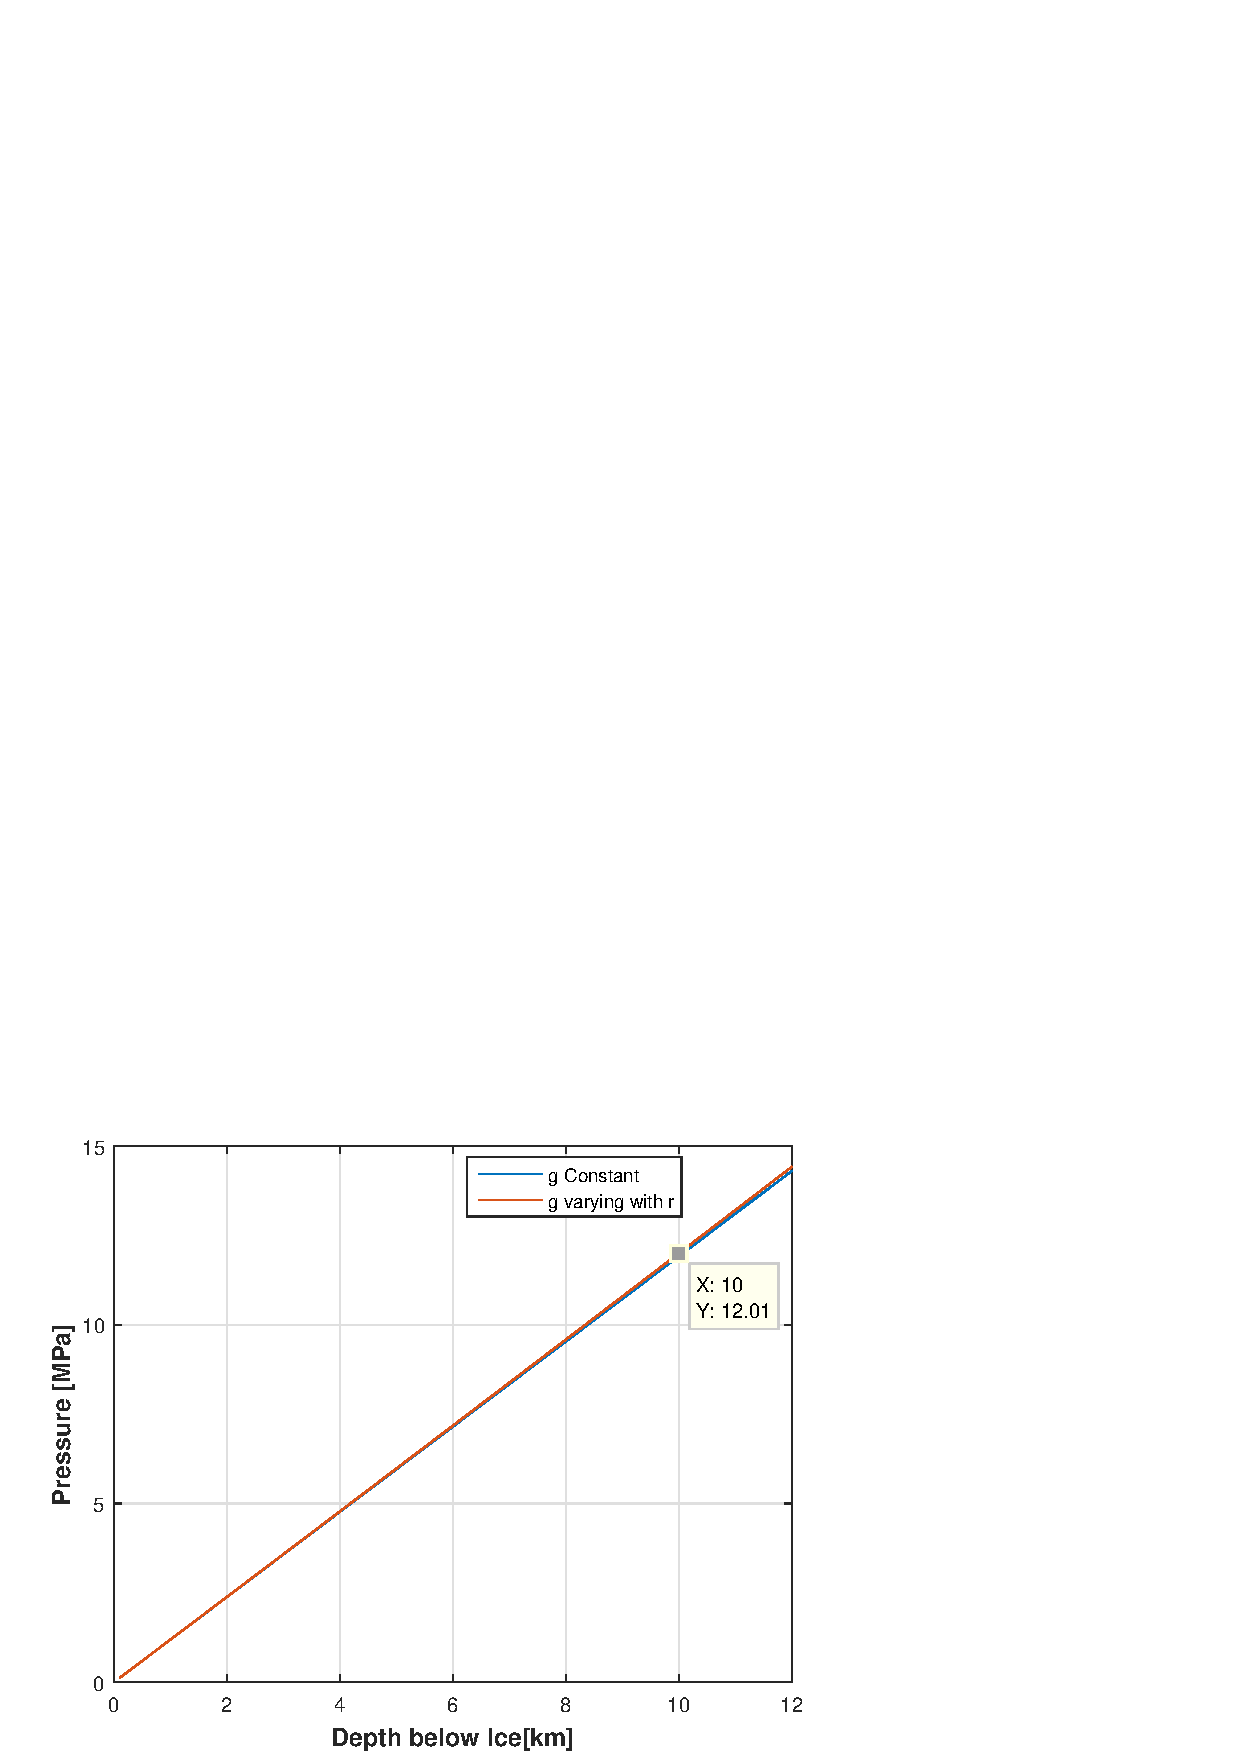
\includegraphics[width=0.48\textwidth]{figures/Orbiter/pressure.png}
        \label{fig:deltaiv_pressure_env}
    }
    \subfloat[Maximum Inner Surface Temperature - Environments to Spacecraft.\cite{Atlasm}]{
        \includegraphics[width=0.48\textwidth]{figures/Orbiter/shell_temp.png}
        \label{fig:deltaiv_temp}
    }
    \caption{Pressure and temperature parameters.}\label{fig:press_temp}
\end{figure}

\begin{figure}[htb]
    \centering
    \captionsetup[subfigure]{width=0.45\textwidth}
    \subfloat[During First-Stage Burn vs. Second Stage Payload Weight.\cite{Atlasm}]{
        \includegraphics[width=0.48\textwidth]{figures/Orbiter/g_staging.png}
        \label{fig:gloads}
    }
    \subfloat[During Second Stage Cutoff.\cite{Atlasm}]{
        \includegraphics[width=0.48\textwidth]{figures/Orbiter/g_2ndstage.png}
        \label{fig:g_2ndstage}
    }
    \caption{Delta IV Heavy Maximum Axial Steady-State Acceleration}\label{fig:accel}
\end{figure}

\begin{figure}[htb]
    \centering
    \captionsetup[subfigure]{width=0.45\textwidth}
    \subfloat[Maximum Spacecraft Separation Shock Level to Launch Vehicle, 1575-5 PAF (95th Percentile, 50\% Confidence).\cite{Atlasm}]{
        \includegraphics[width=0.48\textwidth]{figures/Orbiter/fairing_sep_resp.png}
        \label{fig:fairing_sep_resp}
    }
    \subfloat[Launch-Vehicle-Induced Payload Interface Shock Environment (95th Percentile, 50\% Confidence)—1575-5 Payload Attach Fitting.\cite{Atlasm}]{
        \includegraphics[width=0.48\textwidth]{figures/Orbiter/before_fair_sep.png}
        \label{fig:before_fair_sep}
    }
    \caption{Spacecraft shock environment}\label{fig:shock_env}
\end{figure}

\begin{figure}[htb]
\centering
\includegraphics[scale=0.3]{figures/Orbiter/acoustics.png}
\caption{Delta IV Heavy (5-m Metallic Fairing) Internal Payload Acoustics Typical 95th Percentile, 50\% Confidence Predictions, 60\% Fill Effect Included\cite{Atlasm}.}
\end{figure}

\begin{figure}[htb]
\centering
\includegraphics[scale=0.3]{figures/Orbiter/acceptancelevels.png}
\caption{Acoustic and vibration test requirements\cite{Atlasm}.}
\label{fig:testlevels}
\end{figure}

\subsection{Cruise phase}
The cruise phase is the stage the spacecraft spends between launch and Jupiter arrival. During this 6.4 years period, the spacecraft should remain healthy and every system and science instrument should be designed to survive and be fully operational for the duration of its mission. During the cruise phase 4 flybys are planned, one from Venus, two from Earth and one from Mars. These flybys will provide the additional required to boost the apoapsis of the orbit to Jupiter vicinity. The spacecraft will be equipped with a main engine and smaller Reaction Control System (RCS) thrusters. This propulsion system will be used to perform Trajectory Correction Maneuvres (TCM) to fine tune flyby trajectories. The flybys will also be used as a calibration test of the navigation and geolocalization system of the orbiter which will later be used to map Europa and find potential landing sites. As the mission is planning to flyby Europa multiple times when the Europa reconnaissance phase begins, the interplanetary flybys can be used as a useful analogy to simulate the flyby sequence and identify potential flaws before the actual mission begins. For example, small axis misalignment's of the telescope system with the star tracker’s axis can be spotted using star fields of both telescopic cameras and star trackers and so updating the rotational matrix. This can be done by pointing to a known star fields. Precise knowledge of the spacecraft orientation is crucial for accurate pointing of the cameras while avoiding unintentional pointing of them to the Sun and at the same time keep pointing the high gain antenna to Earth. During cruise, all science instruments will be kept in hibernation mode to eliminate ageing degradation and potential software improvements found post launch will be addressed by software updates. Health checks of the systems will be performed many times during cruise. The cruise phase provides an additional benefit of using the telescope camera for Venus and Mars observations during the flybys as long as potential asteroid flybys on the way to Jupiter. Special attention should be given to the thermal environment of the spacecraft during the flybys, due to the thermal heating of the planets which will be considerably more intense at the Venus flyby. As the emitted energy is calculated using the black body radiation (given by Stefan-Boltzmann law)$L=4\pi R^2\sigma T^4$, where $\sigma$ is the Stefan-Boltzmann constant ($\sigma=5.670373\cdot 10^{-8}  Wm^{-2} K^{-4}$) and T the surface temperature and R the radius of the Sun. As the energy falls by the square of the distance from the source, it can be calculated that the highest solar energy the spacecraft will experience at Venus will be 1.9 times that of the Earth (or 2611 $W/m^2$ ). Given the extra heating from Venus high reflective atmosphere (albedo 0.90), \cite{venus_fact}, and the RTG constant heating, a shade solution should be implemented for the orbiter to keep the temperature to tolerable levels for both electronics and fuel tank temperatures. Some months before Jupiter arrival, the high resolution camera will start an observational campaign of Jupiter’s satellites. The data will be used to update the orbital parameters of the moons and keep uncertainties of their speeds and positions to the lowest level for safety and fuel efficiency of the upcoming flybys and science mission trajectory. During cruise, the spacecraft will be using its high gain antenna pointing towards Earth, at the same time acting as a sun-shield. RTGs generated heat should be dissipated through radiators and carefully monitor fuel tank and temperatures distribution in the spacecraft.
\todo[inline]{add some paragraphs to this section to avoid wall of text}
\subsection{Jupiter orbit insertion phase}
After travelling for six and a half years in interplanetary space, the probe encounters Jupiter sphere of influence. The Hofmann transfer orbit to Jupiter has provided enough energy so the apoapsis of the elliptical orbit will reach Jupiter at the same time that Jupiter is close enough to perform the JOI (Jupiter Orbit Insertion) burn. The telemetry commands for burn are expected to be sent to the spacecraft several days before closest approach. The inclination of the spacecraft incoming trajectory will be close to the Europa orbital plane which is $0.47^\circ$ to Jupiter’s moons plane and $1.79^\circ$ to the ecliptic (source: "Overview of Europa Facts". NASA. )
\todo[inline]{add/fix reference}
. That would be possible from the design of the flybys performed by the spacecraft. A number of small Trajectory Correction Maneuvers (TCM) are expected to be performed during the cruise phase to fine-tune the JOI timing and positioning parameters. The JOI burn starts before closest approach to Jupiter, with the center of the burn happening exactly at the closest approach. Evenly distributing the timing of the burn is important for efficiently reducing the spacecraft’s orbital energy and being able to be capture into Jupiter orbit. The spacecraft enters for the first time the magnetosphere of Jupiter at a distance of 45 to 100 $R_J$, which is the range of the subsolar point of Jupiter’s magnetopause (source: Khurana, K.K.; Kivelson, M. G.; et al. (2004).
\todo[inline]{add/fix reference}
"The configuration of Jupiter's magnetosphere") and is affected by Solar activity. Arriving at solar maximum, the spacecraft will encounter the magnetosphere closer to Jupiter than in a low intensity solar wind period. The JOI burn will take place between the orbits of Europa and Ganymede as this configuration leaves open the possibility of using an initial Ganymede flyby to reduce the required delta-V for Jupiter orbit capture. At the same time, targeting a JOI burn close to Europa minimizes the requirements for a larger post orbit clean-up apoJove burn to bring the periJove of the orbit to Europa’s vicinity. Moreover, the periJove burn at this altitude avoids exposing the spacecraft to the high intensity Jovian radiation belts, the harshest region of them being within 300,000 Km from Jupiter (source: Jupiter Radiation Belts Harsher than expected, March 28, 2001, NASA, JPL).
\todo[inline]{add/fix reference}
An analytical examination of the radiation environment is carried out in Chapter XX, where using SPENVIS models we predict the estimated doses from the high energy protons and electrons. Several minutes before the critical JOI burn take’s place, the spacecraft will re-orient itself for the retrograde burn and thus remain out of high-gain antenna contact with Earth during the duration of the burn (LOS). At that time, a smaller low gain antenna will be used to provide tone signals relaying vehicle status. 
\subsection{Jupiter Orbit Insertion delta-V calculation}
A limiting factor in the mission is the total payload that can be brought to Europa. Before that, the spacecraft should be captured in orbit around Jupiter. We investigate the amount of fuel such a maneuver will require, having in mind that the upper mass limit is defined by our launcher vehicle, which will be the Atlas IV Heavy with the maximum payload capability of 7389Kg as calculated in table \ref{tab:trajKg}.

The spacecraft arrives at Jupiter in a hyperbolic trajectory. Jupiter gravity becomes important at the sphere of influence radius of Jupiter (see Chapter XX)
\todo[inline]{add/fix reference}
, which is around 48 million Km. The hyperbolic excess velocity can be expressed as the difference of the spacecraft trajectory at the apoapsis of its Hohmann transfer orbit $V_(SC,A)$ and Jupiter’s orbital speed $V_J$:
\begin{equation}
V_\infty=V_{SC,A}-V_J
\end{equation}

\begin{figure}[htb]
\centering
\includegraphics[scale=0.3]{figures/Orbiter/capture.png}
\caption{Incoming asymptote trajectory to Jupiter (Howard D. Curtis, Orbital Mechanics for Engineering Students).\cite{orbitals}}
\label{fig:capture}
\end{figure}

The approach hyperbolas for a specific flyby are varying according to their aiming radius $\Delta$ as can be seen in figure \ref{fig:joihyp}. Our mission incoming asymptote will have a periapsis radius which in our case will be between the orbits of Europa and Ganymede, at radius of $r_p=865000km$ (12$R_J$) from Jupiter. At this point, the first steps is to be captured into Jupiter orbit with the lowest amount of propellant spent. This will allow the mission to carry more effective payload to Europa. 

\begin{figure}[htb]
\centering
\includegraphics[scale=0.3]{figures/Orbiter/joihyp.png}
\caption{Incoming hyperbolas for varying aiming radius (Howard D. Curtis, Orbital Mechanics for Engineering Students).\cite{orbitals}}
\label{fig:joihyp}
\end{figure}

To get into orbit, the spacecraft needs to fire its engine in the anti-velocity (retrograde) direction and remove the excess delta-V at the hyperbolic periapsis. The amount of delta-V reduction is depending on the type of capture orbit we want to achieve. In our case, the most fuel efficient option will be a highly eccentric orbit (e=0.9) around Jupiter with an orbital period of 165 days. The speed at the periapsis of hyperbolic trajectory is given by the formula:
\begin{equation}
V_{hyp,p}=\sqrt{V_{\infty}^{2}+\frac{2\mu}{r_p}}
\end{equation}
Where $\mu=GM_J$ is the gravity parameter for the Jupiter two body problem. The required speed for an elliptical Jupiter capture orbit is given by the orbital dynamics equations by the formula:
\begin{equation}
V_{capture}=\sqrt{\frac{\mu\left(1+e\right)}{r_p}}
\end{equation}
The difference of the above velocities will give us the required delta-V for Jupiter orbit capture. Note that in these calculations, the incoming asymptote of the Hohmann transfer orbit in the Jupiter reference system is parallel to Jupiter’s orbital track and so the vector subtraction of Jupiter’s orbital and spacecraft asymptotic velocities equals with the absolute values of the velocities subtraction.  Doing, the delta-V calculation for the hyperbolic excess velocity given by Petropoulos et al. for the VEMEGA orbit
\todo[inline]{add/fix reference}
($V_\infty=5.58km/s$) we get:
\begin{equation}
\Delta V_{capture}=\sqrt{V_{\infty}^{2}+\frac{2\mu}{r_p}}-\sqrt{\frac{\mu\left(1+e\right)}{r_p}} = \mathbf{1.321 [km/s]}
\end{equation}
\subsection*{Fuel mass calculation}
To calculate the fuel consumption for the required delta-V burn, we use the general rocket thrust equation:
\begin{equation}
F = \dot{m}v_e+(p_e-p_o)A_e
\end{equation}
Where the following engine parameters are required:
\begin{equation}
\begin{split}
\dot{m}&:\text{fuel mass rate}\\
v_e&:\text{equivalent velocity-exit velocity}\\
p_e&:\text{exit pressure}\\
p_o&:\text{free stream pressure}\\
A_e&:exit/nozzle \text{ area ratio}\\
\end{split}
\end{equation}

\begin{figure}[htb]
\centering
\includegraphics[scale=0.6]{figures/Orbiter/rockth.png}
\caption{Thrust equation schematic diagram (Source:NASA, GRC).\cite{rocketeq}}
\label{fig:rocketim}
\end{figure}

Dividing the thrust equation with the mass rate, we define the equivalent velocity:
\begin{equation}
v_{eq}=\frac{F}{\dot{m}}=v_e+\frac{(p_e-p_o) A_e}{\dot{m}}
\end{equation}
Then, we define the specific impulse parameter, which describes the ratio of thrust produced to the weight of propellant, in seconds using the updated thrust equation:
\begin{equation}
I_{sp}=\frac{v_eq}{g_o} =\frac{F}{\dot{m}g_o}
\end{equation}
Thus, substituting to the thrust equation, we get the thrust written as:
\begin{equation}
F=I_{sp}\dot{m}g_o
\end{equation}
We then employ Newton’s second law of motion:
\begin{equation}
F=m\frac{du}{dt}
\end{equation}
\begin{equation}
\int_{u_o}^{u}du=-\int_{m_o}^{m}\frac{I_{sp}g_o}{m}dm
\end{equation}
So, the total velocity change can be expressed as:
\begin{equation}
\Delta v=-I_{sp}g_o ln(\frac{m}{m_o})
\end{equation}
The final mass of the spacecraft after the required delta-V change will then be:
\begin{equation}
m_{final}=m_{o}e^{-\frac{\Delta v}{v_{eq}}}
\end{equation}
\subsection*{Spacecraft propulsion}
In order to get a realistic fuel required calculation for the JOI burn, we are using an analog of the propulsion system used in the Cassini spacecraft. The total wet mass of the Cassini-Huygens mission was 5574Kg and used two engines, one for redundancy.
\todo[inline]{add/fix reference}
Cassini's engine characteristics and the Europa Lander Mission are shown in the following board:
% Table generated by Excel2LaTeX from sheet 'Ark1'
\begin{table}[htb]
  \centering
    \begin{tabular}{|c|c|c|}
    \hline
          & \textbf{Cassini} & \textbf{Europa Lander Mission} \bigstrut\\
    \hline
    Engine Thrust (N) & 440   & \textbf{500} \bigstrut\\
    \hline
    Engine Isp (s) & 308   & \textbf{300} \bigstrut\\
    \hline
    Spacecraft wet mass (Kg) & 5574  & \textbf{7300} \bigstrut\\
    \hline
    \end{tabular}%
    \caption{Cassini propulsion comparison.}
  \label{tab:propulsion}%
\end{table}%
Using the engine thrust equations, the calculated fuel mass for the JOI burn has the requirements specified in table (\ref{tab:joi_burn}).
% Table generated by Excel2LaTeX from sheet 'Sheet1'
\begin{table}[htb]
  \centering
    \begin{tabular}{|c|c|c|}
    \multicolumn{3}{c}{\textbf{JOI burn requirements }} \bigstrut[b]\\
    \hline
    \textbf{} & No initial Ganymede flyby & Initial Ganymede flyby \bigstrut\\
    \hline
    \textbf{Engine Thrust Efficiency} & 100\% & 100\% \bigstrut\\
    \hline
    \textbf{DeltaV Magnitude (Km/s)} & 1321  & 921 \bigstrut\\
    \hline
    \textbf{Burn duration (min)} & 262.7 & 197.6 \bigstrut\\
    \hline
    \end{tabular}%
  \label{tab:joi_burn_req}%
\end{table}%
\subsection*{Possibility of initial Ganymede pump-down flyby}
In order to further reduce the calculated propellant mass required for the JOI burn, there is the possibility of using an initial Ganymede flyby. A flyby at 500Km altitude from Ganymede will save about 400 Km/s of delta-V (Europa Study 2012 Report, NASA, Europa Study Team) 
\todo[inline]{add/fix reference}
which translates to 928Kg of fuel saved for our mission. As the fuel saving is significant, the Europa Lander Mission will use the initial Ganymede flyby. The time coordination of the Ganymede flyby will be further redefined from the pre-arrival Jupiter moons observation campaign and small TCM burns several months before arrival to Jupiter.
\todo[inline]{Add table references to the section, as tables will move around! Double check label names and references!}
\begin{table}[htb]
  \centering
    \begin{tabular}{|c|c|c|}
    \hline
    \textbf{} & No initial Ganymede flyby & Initial Ganymede flyby \bigstrut\\
    \hline
    \textbf{Engine Thrust Efficiency} & 100\% & 100\% \bigstrut\\
    \hline
    \textbf{DeltaV Magnitude (Km/s)} & 1321  & 921 \bigstrut\\
    \hline
    \textbf{Burn duration (min)} & 262.7 & 197.6 \bigstrut\\
    \hline
    \textbf{Fuel used (Kg)} & \textbf{2642} & \textbf{1963} \bigstrut\\
    \hline
    \end{tabular}%
    \caption{JOI burn requirements}
  \label{tab:joi_burn}%
\end{table}%

\begin{figure}[htb]
\centering
\includegraphics[scale=0.25]{figures/Orbiter/JOIcloseup.png}
\caption{Simulation of the JOI burn sequence (Ifikratis Kamenidis, STK Software).}
\label{fig:joicloseup}
\end{figure}

\begin{figure}[htb]
\centering
\includegraphics[scale=0.4]{figures/Orbiter/JOIfull.png}
\caption{Simulation of the JOI burn sequence and 165 days capture orbit (Ifikratis Kamenidis, STK Software).}
\label{fig:joifull}
\end{figure}

For figures (\ref{fig:joicloseup}), (\ref{fig:joifull}), the STK software was used to simulate and test our calculations for the JOI burn. The Summary report of the calculation agrees with our estimated parameters:

\begin{figure}[htb]
\centering
\includegraphics[scale=0.5]{figures/Orbiter/captorb.png}
\caption{STK Orbital period calculation report before and after JOI. The simulation agrees with the 165 days target initial orbit(Ifikratis Kamenidis, STK Software).}
\end{figure}

\begin{figure}[htb]
\centering
\includegraphics[scale=0.5]{figures/Orbiter/JOIres.png}
\caption{Summary report of JOI burn.(Ifikratis Kamenidis, STK Software).}
\end{figure}
\todo[inline]{remember label, reference to the above figures.}

\subsection{Jupiter Capture Orbit}
 The selection of the equatorial plane for the Jupiter orbit insertion was done based on the orbiter's mission goals, which is to characterise Europa’s through multiple flybys and deploy a lander into its surface. The only viable way from an orbital mechanics point of view to intercept Europa many times, achieve a good surface coverage before landing and deploy a lander using the least amount of carrying fuel is a by using a low -relative to Europa- inclination orbit around Jupiter. While a polar orbit would better avoid the high radiation lobes of the Jupiter magnetosphere, the above criteria could not be met. An orbit around Europa was ruled out based on the extremely high radiation levels. The JOI burn was designed taking into account the above orbital mission requirement while saving fuel using the opportunity of an initial Ganymede flyby. The capture orbit parameters, and especially the eccentricity of 0.6 was chosen as a realistic trade-off between orbital period and fuel required. A higher eccentricity orbit would require less fuel but would lead to a very high orbital period around Jupiter, prolonging the start of the Europa mission for more than 2 years. On the other hand a lower eccentricity orbit would spare a significant amount of fuel to lower the eccentricity.
\subsection{Post-Capture orbital design}
Right after the successful completion of the 197min JOI burn, the spacecraft has been captured in the initial 165 days orbit. However, the missions goal's wouldn't be achieved by staying in this long period orbit. The orbital plan is to use the more massive of the Jovian satellites, Ganymede multiple times to slow the spacecraft down and bring it to a Europa 3:1 resonant orbit around Jupiter. For this scenario to be successful, the spacecraft should use a minimum amount of fuel to fine tune the Ganymede flybys and achieve most of the $\Delta V$ reduction from the close Ganymede encounters. 
\subsection{Post-Capture orbits progression analysis}
Just by letting the spacecraft orbit Jupiter in a 165 days orbit, will require significant amount of fuel to target a Ganymede flyby, as the relative positions of the spacecraft and Ganymede would be completely random. For that reason, the JOI burn and arrival time are properly targeted during cruise's TCM so that the spacecraft will pass close to Ganymede in the first inbound leg of the capture orbit just before it completes its first 165 orbit. However, the JOI burn and a potential initial Ganymede flyby create unavoidably a post-capture $\Delta V$ error. This  error would be easy to take out in the first apoJove pass, targeting the first Ganymede post-orbit pump-down flyby. At this point, the amount of $\Delta V$ required to plan the Ganymede flyby is small enough (see analysis later XX) to easily achieve a very close Ganymede flyby and so achieve the maximum $\Delta V$ reduction. However, thinking more wisely, such a manoeuvre will not result in the maximum fuel efficiency at the long term. The resulting orbit will then need a significant amount of fuel to plan a next Ganymede (or other moon) flyby, as the orbits will again be chaotic. Spending a huge amount of fuel will unpredictably add mass to the mission while on the other hand, waiting for many orbits for a next opportunity will shift the mission lifetime and risk its successful completion, mainly because of the accumulating radiation of Jupiter's magnetosphere.

It is evident that a more ahead-planning scenario is required. We solve this problem by performing the initial Ganymede flyby in a more reasonable way. Instead of trying to achieve the maximum $\Delta V$ reduction, we plan the first Ganymede flyby in the right aiming radius for a resulting Ganymede resonant orbit. By doing so, we make sure that the next orbit will not be random, but will have an orbital period which will be an integral multiple of Ganymede's orbit around Jupiter (Ganymede resonant orbit). This coherence, assures that the spacecraft can use Ganymede again for a further $\Delta V$ reduction in the next orbit with no fuel required. By repeating the same scheme for the 2nd Ganymede flyby, the spacecraft is again on track for a next flyby. Any excess post flyby $\Delta V$ is managed in the apoJove pass, where a small burn is performed to fine-tune the upcoming flyby. The above orbital design will allow the spacecraft to flyby Ganymede every time with the least amount of fuel. After an achieved resonance of 4:1, a flyby with Europa is within reach, and by performing small burns the final Europa resonance orbit will be achieved. 
\subsection{Post-Capture manoeuvres and fuel mass calculations}
In order to test the post-capture orbits scenario viability and perform a detailed analysis of the fuel required for the correction manoeuvres, the STK software (version 10.1.3), a physics-based software geometry engine. For the orbits simulations the Astrogator (v10.0) extension was used. 

Except Jupiter, the four largest Jovian moons gravity models was used in the simulation, to accurately simulate perturbation effects in the orbits evolution. A 7th order Runge-Kutta-Fehlberg integrator with 8th order error control with 1 sec minimum stepsize was used to propagate the spacecraft's motion in Jupiter's gravity field as well as during the Sphere of Influence of Ganymede and Europa when their specific gravity fields were used (see sphere of influence). The gravity fields used can be seen in table (\ref{tab:gravf}). Furthermore, a spherical solar radiation pressure (SRP) is used with a dual-cone shadow model.

% Table generated by Excel2LaTeX from sheet 'Sheet1'
\begin{table}[htb]
  \centering
    \begin{tabular}{|c|c|c|c|}
    \hline
    \multicolumn{4}{|c|}{\textbf{Gravity models}} \bigstrut\\
    \hline
    \textbf{Object} & \textbf{Gravity Model} & \textbf{Degree} & \textbf{Order} \bigstrut\\
    \hline
    \textbf{Jupiter} & JUP230.grv & 6     &  \bigstrut\\
    \hline
    \textbf{Io} & JUP230.grv & 6     &  \bigstrut\\
    \hline
    \textbf{Europa} & Science1998.grv & 4     & 2 \bigstrut\\
    \hline
    \textbf{Ganymede} & Nature1996.grv & 4     & 2 \bigstrut\\
    \hline
    \textbf{Callisto} & JUP230.grv & 6     &  \bigstrut\\
    \hline
    \end{tabular}%
    \caption{Gravity models used in simulation(source: NASA, Horizons, NAIF).\cite{Gravm}}\label{tab:gravf}
\end{table}%

In order to perform the required orbits and manoeuvres calculations by the simulation engine, a series of commands are written in a logical sequence. The software uses a differential corrector to solve a problem of initial conditions, given a set of orbital goals. 
The core of the commands can be synopsised in the following sequence:

\begin{itemize}
  \item Propagate at orbit apoJove
  \item Initiate burn - 3 degrees of freedom
  \item Propagate at Ganymede Sphere of Radius
  \item Target flyby B-plane - specific BdotR, BdotT goals are set
  \item Propagate at apoJove
\end{itemize}

At the end of each iteration, the resulting orbital period is checked. BdotR and BdotT targets are altered until the desired orbital period is achieved. Then, the same iteration sequence is run for calculating the upcoming Ganymede flyby. The achieved resonances or orbit two, three and four (orbit one equals to capture orbit) are 9:1, 6:1 and 3:1 respectively. 
\todo[inline]{Consider replacing BdotR with $B\cdot R$ in the above}
Table (\ref{tab:boardm}) shows an overview of the apoJove burns and flyby $\Delta V$ parameters.

% Table generated by Excel2LaTeX from sheet 'Sheet1'
\begin{table}[htb]
  \centering
    \begin{tabular}{|r|r|r|r|r|}
    \hline
          & \boldmath{}\textbf{$\Delta V (m/s)$}\unboldmath{} & \textbf{Burn time(s)} & \textbf{Fuel used (Kg)} & \textbf{Range (Km)} \bigstrut\\
    \hline
    \multicolumn{1}{|c|}{\textbf{O1-B1}} & \multicolumn{1}{c|}{4.409015} & \multicolumn{1}{c|}{29.926} & \multicolumn{1}{c|}{8.114} & \multicolumn{1}{c|}{} \bigstrut\\
    \hline
    \multicolumn{1}{|c|}{\textbf{G1}} & \multicolumn{1}{c|}{794.84} & \multicolumn{1}{c|}{} & \multicolumn{1}{c|}{} & \multicolumn{1}{c|}{2268} \bigstrut\\
    \hline
    \multicolumn{1}{|c|}{\textbf{O2-B2}} & \multicolumn{1}{c|}{0.724688} & \multicolumn{1}{c|}{4.919} & \multicolumn{1}{c|}{1.334} & \multicolumn{1}{c|}{} \bigstrut\\
    \hline
    \multicolumn{1}{|c|}{\textbf{G2}} & \multicolumn{1}{c|}{494.89} & \multicolumn{1}{c|}{} & \multicolumn{1}{c|}{} & \multicolumn{1}{c|}{3189} \bigstrut\\
    \hline
    \multicolumn{1}{|c|}{\textbf{O3-B3}} & \multicolumn{1}{c|}{4.197475} & \multicolumn{1}{c|}{28.49} & \multicolumn{1}{c|}{7.725} & \multicolumn{1}{c|}{} \bigstrut\\
    \hline
    \multicolumn{1}{|c|}{\textbf{G3}} & \multicolumn{1}{c|}{1223.24} & \multicolumn{1}{c|}{} & \multicolumn{1}{c|}{} & \multicolumn{1}{c|}{489} \bigstrut\\
    \hline
    \multicolumn{1}{|c|}{\textbf{O4-B4}} & \multicolumn{1}{c|}{1.180696} & \multicolumn{1}{c|}{8.014} & \multicolumn{1}{c|}{2.17} & \multicolumn{1}{c|}{} \bigstrut\\
    \hline
    \multicolumn{1}{|c|}{\textbf{G4}} & \multicolumn{1}{c|}{1080.2} & \multicolumn{1}{c|}{} & \multicolumn{1}{c|}{} & \multicolumn{1}{c|}{497} \bigstrut\\
    \hline
    \multicolumn{1}{|c|}{\textbf{O5-B5}} & \multicolumn{1}{c|}{103.7305} & \multicolumn{1}{c|}{1146} & \multicolumn{1}{c|}{187.376} & \multicolumn{1}{c|}{} \bigstrut\\
    \hline
    \multicolumn{1}{|c|}{\textbf{E1}} & \multicolumn{1}{c|}{804.61} & \multicolumn{1}{c|}{} & \multicolumn{1}{c|}{} & \multicolumn{1}{c|}{627} \bigstrut\\
    \hline
    \multicolumn{1}{|c|}{\textbf{O6-B6}} & \multicolumn{1}{c|}{149.8431} & \multicolumn{1}{c|}{1644} & \multicolumn{1}{c|}{256.233} & \multicolumn{1}{c|}{} \bigstrut\\
    \hline
    \multicolumn{1}{|c|}{\textbf{E2}} & \multicolumn{1}{c|}{45.98} &       & \multicolumn{1}{c|}{} & \multicolumn{1}{c|}{3771} \bigstrut\\
    \hline
    \multicolumn{1}{|c|}{\textbf{Total }} & \multicolumn{1}{c|}{4707.8} &       & \multicolumn{1}{c|}{462.952} & \multicolumn{1}{c|}{} \bigstrut\\
    \hline
    \end{tabular}%
    \caption{Resulting burn parameters for post-Jupiter capture orbits progression. Assumed 5426Kg wet mass after JOI burn in the Ganymede initial pump-down scenario. The new wet mass after a burn is always taken into account in the calculations.Engine ISP=300s and Engine thrust=500N. OX-BX indicate the apoJove burns, while with GX and EX are noted the in sequence Ganymede and Europa flybys.}
  \label{tab:boardm}%
\end{table}%

\begin{figure}[htb]
\centering
\includegraphics[scale=0.6]{figures/Orbiter/orbits.png}
\caption{Orbits evolution from JOI to Europa target 3:1 resonance orbit. (Ifikratis Kamenidis, STK Software).}\label{fig:orbits_resonance}
\end{figure}

\subsection{Arriving at target orbit}
After the completion of the first two Ganymede flybys, the third Ganymede flyby is performed with a dual purpose. First to further reduce the apoJove distance of the orbit and at the same time place the spacecraft in an orbit to intercept Europa for the first time. Meanwhile, every Ganymede flyby is lowering the periJove of the orbit, while the last Ganymede flyby brings the periJove at approximately 9.3 $R_J$ in Europa's vicinity. The first Europa flyby itself is designed to provide the necessary $\Delta V$ reduction to place the spacecraft in the target 3:1 resonant Europa orbit. For every one spacecraft orbit around Jupiter, Europa make exactly three orbits. This synchronisation is key in achieving a continuous flybys in order to provide the orbiter the ability to do pre-landing reconnaissance and find the best landing site location for the lander module. After landing the same orbit will be used to provide the communication link between the penetrator -lander and the Earth. The orbital parameters of the target orbit can be seen in table (\ref{tab:eurorb}).

% Table generated by Excel2LaTeX from sheet 'Sheet1'
\begin{table}[htb]
  \centering
    \begin{tabular}{|c|c|}
    \hline
    Semi-major axis (Km) & \textbf{1,392,748} \bigstrut\\
    \hline
    PeriJove (Km) & \textbf{662,300} \bigstrut\\
    \hline
    ApoJove (Km) & \textbf{2,525,000} \bigstrut\\
    \hline
    Eccentricity & \textbf{0.5244} \bigstrut\\
    \hline
    Inclination ($^\circ)$ & \textbf{3.816} \bigstrut\\
    \hline
    Period (days) & \textbf{10.6} \bigstrut\\
    \hline
    TID under 2cm of Al (krad/month) & \textbf{5.2} \bigstrut\\
    \hline
    Europa flyby relative $\Delta V$(Km/s) & \textbf{3.3} \bigstrut\\
    \hline
    \end{tabular}%
    \caption{Europa 3:1 resonant orbit parameters.}
  \label{tab:eurorb}%
\end{table}%
\begin{figure}[htb]
\centering
\includegraphics[scale=1]{figures/Orbiter/europares.png}
\caption{Europa 3:1 resonant orbit (Ifikratis Kamenidis, STK Software).}
\end{figure}
\todo[inline]{Double check all figure/table references! Make sure figures has not moved}
\subsection{Perturbations and orbit sustainability}
Keeping the spacecraft to the 3:1 Europa resonant orbit around Jupiter would require a significant amount of fuel. Europa's mass is significant enoughh to alter the spacecraft's trajectory every time it flies by the moon. The gravity assist was extremely useful for the initial pump-down and orbital decay of the capture orbit as explained in the previous chapters. However, in the case of the target orbit, unavoidably a $\Delta V$ change will occur after every flyby. As a result, the apojove radius will now change, hence the orbital period and the resonance geometry. An apojove burn will be necessary in every orbit to keep the spacecraft in the resonant trajectory. In that case the amount of fuel required will be very large. Moreover, besides sustaining the orbit the goal of the orbiter's flyby is to map the surface prior to landing, and so a method of placing the groundtrack of a hyperbolic orbit over desired latitudes and longitudes has been developed by NASA (REFERENCE)
\subsection{Communication windows}
\todo[inline]{STK differential corrector theory}
\todo[inline]{Sphere of Influence}
\todo[inline]{Flyby B-plane targeting}
\input{Orbiter/3b_implementation_orbit.tex}
\autchapter{Analysis of the Surface Environment}{Paschalis Dalampiras, Ifikratis Kamenidis, and Johannes Linde}\label{ch:surf_env}
%\section{Analysis of Europa Moon surface and Environment}
\section{The Radiation Environment}\label{sec:radiation_environment}
Jupiter’s magnetic field, shaped as a toroidal, affects the radiation environment around the planet by interacting with the solar wind trapping energetic particles, creating radiation belts similar to van Allen belts on Earth but with much higher intensity. This magnetosphere of charged particles extends radially from 50 to 100 RJ. For purpose of practicality this area is subdivided into three main regions, the outer magnetosphere ($>$40 RJ), middle (10-40 RJ) and the inner magnetosphere ($<$10 RJ). For our purpose, we are focusing on the middle region, an area where Europa lays along with the rest of the four Galilean moons, Io, Ganymede and Calisto. Highly energetic charged particles are trapped within that region, mainly electrons and protons but also ions, ranging from a few keV up to tens of MeV. Here we can also locate the Io plasma torus, created by the interaction of the rotating magnetic field of Jupiter with the spewed volcanic gasses of Io, drifting and ionizing them into plasma.

Axial tilt of the magnetic dipole of Jupiter and consequently of the spin plane, causes Europa to cruise in and out of the plane by 10o north and south of the magnetic latitude affecting the radiation environment of the moon. 

Through a process known as sputtering, bombardment of Europa’s surface with highly ionizing particles causes the ejection of surface molecules where some of them manage to escape gravitational pull of the moon and get accelerated by the co-rotating magnetosphere creating an additional contribution to the particle distribution. 

Data collected by Galileo, Voyager and Pioneer spacecraft missions show high intensities of energetic particles fluxes around Europa’s orbit area varying in time to a limited extent. Electrons intensity (fig. \ref{electrons energy}) show a wide spectra of energies dominating on that region but with a large variation on lower energies due to the high uncertainty rates of the detectors during these missions and especially from Galileo.
\begin{figure}[htb]
\centering
\includegraphics[width=0.5\textwidth]{figures/Orbiter/electrons_energy_spectrum}
\caption{Energy spectrum of electrons near Europa’s orbit from various sources, \cite{paranicas2009europa}.}
\label{electrons energy}
\end{figure}
Several Galileo close encounters to Europa’s orbit, reveal the energy distribution of proton, oxygen and sulfur ions and show high intensities at high energies while on low energies a greater variation between the ions is observed (fig. \ref{fig:ions_energy}).
\begin{figure}[htb]
    \centering
    \includegraphics[width=0.80\textwidth]{figures/Orbiter/ions_energy}
    \caption{Ion energy spectra data acquired from Galileo mission on various encounters of Europa at distances of 692 km (E4), 586 km (E6), 201 km (E12), 1439 km (E19), and 351 km (E26) \cite{paranicas2009europa}}
    \label{fig:ions_energy}
\end{figure}
\section{Current Studies of the Surface}\label{sec:surface_studies}
Delivering a lander vehicle on Europa, requires a thorough knowledge of the surface composition and characteristics. On a large scale the surface looks smooth and without great variations but on a higher spatial resolution we can notice the complexity of the terrain. Smooth plains, lenticulae and chaos regions dominate the morphology and topography of the moon’s surface. Many models have suggested that formation of these terrain features involves hydrothermal activity within the ice shell causing fractures and ridges (fig\ref{fig:europa_surface}). 
\begin{figure}[htb]
    \centering
    \includegraphics[scale=0.6]{figures/Orbiter/europa_surface.png}
    \caption{Left: Europa’s trailing (top) and leading (bottom) hemispheres as imaged from Galileo on the left and enhanced on the right to illustrate the geological complexity of the surface. Right: A close up look of the surface \cite{carlson2009europa}}
    \label{fig:europa_surface}
\end{figure}
Studies of the surface composition, suggest that Europa was formed by endogenic and exogenic sources of materials. Endogenic sources include either thermochemical reactions that have created hydrated silicates, iron oxides and carbon-nitrogen compounds or unaltered silicates, nickel-iron compounds, organic matter and water, depending on the initial conditions of the protojovian nebula. As for exogenic material, three main sources have been identified. Io’s ejected material reaching Europa by its thermal plasma torus, material outside of the Jovian system delivered by comets and asteroids, and material from the outer Jovian satellites ejected from their surfaces.
%\todo[inline]{Other missions - Galileo et al.}
\section{Lenticulae}\label{sec:lenticulae}
On the surface of Europa a number of circular and elliptical formations are observed, named as lenticulae (fig. \ref{fig:lenticulae}). Many of these are domed hills, cavities and others seems to be dark and flat blemishes. Some appear to have a rough surface with a chaotic structure. The peaks of these domes, show similarities with the composition of the nearby surface, indicating that they have been probably created when the crust forced from below due to some geological events, similar to the magma chambers on Earth. Origin of the flat dark blemishes seems to be melted ice that has been released from cracks of the surface.
\begin{figure}[htb]
    \centering
    \includegraphics[scale=0.3]{figures/Orbiter/lenticulae.jpg}
    \caption{Lenticulae on Europa's surface / Courtesy of Galileo Project, NASA}
    \label{fig:lenticulae}
\end{figure}
\section{Chaos regions}
About one quarter of Europa’s surface is covered by highly disrupted areas mostly known as chaotic regions.  Most of these chaotic regions are concentrated in two oval shaped areas within 40$^{\circ}$ of the equator and centred at 120$^{\circ}$ and 300$^{\circ}$ W probably because these areas correspond to the location of paleopoles before the reorientation event, where tidal heating is more active. Also regions like Thera Macula, a low lying area with possible subsurface water, provide an indication of present active chaotic formation. Morphologically, chaos regions can vary presenting distinct characteristics or even combinations of them.

Plates of preexisting terrain are characterised by a spanning between 1-20km across, usually elevated from the surrounding area or with one of their edges tilted. Reconstruction models have shown that most of these plates have moved from their original positions, with 22\% of them showing a movement of over 5km. Other areas present inward facing scarps, slopes extending upwards into their neighbour terrain or even signs of chaotic terrain flowing into nearby ridges.
Numerous existing models have tried to describe the geophysical process of formation of these regions with the melting through the icy shell and brine mobilization models being the predominant, managing to explain most of the key and secondary observations. Melting through the icy shell model suggests that heat originating from the seafloor manages to melt the ice crust creating pits beneath the surface ice, while brine mobilization includes materials with low melting point conducting heat within the ice, lowering its viscosity and allowing leakage of liquids through the shell. Other models propose exogenic impacts on the surface as a mechanism of chaos region creation, while rising diapirs may be used to explain some large dome features.  
\begin{figure}[htb]
    \centering
    \includegraphics[scale=0.3]{figures/Orbiter/chaos.png}
    \caption{Conamara Chaos, Galileo E6ESBRTPLN01 observation \cite{chaosterrain}}
    \label{fig:conamara_chaos}
\end{figure}
Something that characterize the surface of these regions, is their distinctive dark red-brown color. Origin and exact composition of the material present on these area is still under investigation since not enough data are available but some estimations predict that probably is originating from sulfur compounds produced via radiolysis on the surface. Additionally spectral analysis of the same region on the infrared spectra, indicates the presence of a hydrated material like sulfate salts or sulfuric acid hydrate. If this estimation is confirmed then the low melting point of these materials, compared to the one of pure water ice, adds an important aspect in the formation of the chaos regions.
\begin{itemize}
    \item Avoid certain areas (brown areas, chemical compositions)
\end{itemize}
\todo[inline]{Resolution provided by current imaging from casini and imaging spectrometers?}
\todo[inline]{Is 30 percent a realistic coverage? Why? Give a rough estimate of the suitable landing zones. }


\autchapter{Orbiter and Imaging System}{Johannes Linde, Ifikratis Kamenidis, and Paschalis Dalampiras}
%\section{Introduction}
%\todo[inline]{Introduction to the Europa Moon Surface/environment}
\todo[inline]{Brief Purpose of the Reconnaissance Imaging System}
\todo[inline]{Define limits and boundaries (the whole orbiter will not be designed)}
\section{Analysis of ERIS}
\section{Analysis of the Imaging System}
The Europa Reconnaissance Imaging System (ERIS) plays an important role in the first phases of the mission. During the early stages, the imaging system will be used to map the surface of Europa and provide the necessary data for selecting a suitable landing site for the lander and penetrator. At this point, it is expected to have one or more cameras on the orbiter, mapping the surface of Europa in both low and high resolution. 
%\section{The Strawman Mission}
\subsection{The purpose of ERIS}
The Imaging System will be located in the orbiter, performing its primary objectives during the early stages of the life finding mission mission and performing the secondary objectives after a successful landing on Europa.

It is expected that the imaging system will be the main (and only) source of up-to-date, high resolution images throughout the mission. Therefore, it will be the only provider of the data that can be used for selecting a suitable landing site for the Europa Lander. It is assumed, that the current images provided from the Galileo Missions does not provide a high enough resolution to select a suitable landing site. This is the main reason why the relatively costly imaging system is required to perform additional mapping of the surface. 
\todo[inline]{Provide source for this assumption, i.e. the resolution is too low using the sources from Galileo. Image examples?}
\subsection{Landing Site Selection}
During the first phase of the mission, the Imaging System will map the surface. The purpose of the mapping is to provide enough information about the surface, to ensure a suitable landing site can be selected and to ensure the landing will be successful. When selecting the landing site, the following criteria will be considered:
\begin{description}
    \item[Roughness and Elevation] The roughness of the surface can be a great danger for the lander. Large boulders can be fatal, blocking the penetrator from touching the ice or causing misalignment. Boulders can also cause the lander to flip, after an otherwise successful landing. Surface elevation is also very dangerous for the mission - too steep, and the lander can topple over, ending the mission immediately. Therefore, it is necessary to investigate technologies, that can be used to map the surface in high resolution, ensuring large objects can be identified and avoided, making it possible to land on a relatively flat surface.
    
    While high resolution imaging will make it possible to identify dangerous objects, it may not be possible to create topographic data of the lunar surface, unless the cameras are operated in stereo. Therefore, these technologies will also be investigated.
    \item[Radiation] Some areas of the moon have a lower radiation, making them more suitable for the landing site. These areas were discussed previously, in section (\ref{sec:radiation_environment}).
    \item[Chemistry] The current knowledge about the surface chemistry of Europa is very limited. However, spectroscopic data from the Galileo NIMS spectrometer hints that sulphur-rich regions exists. To investigate the surface chemistry, multispectral imaging should be investigated further, as it can provide data about the surface composition of Europa. Knowledge about the surface chemistry is necessary, as some regions may be very unsuited for a landing site, due to the hazardous chemical compounds that are expected in these areas.
    \todo[inline]{Refer to the previous section about surface composition. }
    \item[Proximity to ocean] Naturally, the selected landing site should be close to the ocean, as it is expected that the ice thickness (and therefore mission duration) will vary, depending on the selected landing site.
    
    Ice sounding radars are normally used for assessing the ice structure but this analysis has focus on technologies, that can be used to enhance the imaging system. In addition to surface material assessment, recent papers suggest that spectroscopic data can also be used for analysing the ice surface\cite{naegeli2015a}.
    \item[Communication window] The communication window will be affected by the choice of landing site.
    \todo[inline]{Communication Window. more to add Ifikratis}
\end{description}
\subsection{Manual vs. Automatic selection}
Due to the limited bandwidth, it is not realistic to transmit all the high resolution images back to earth, before the lander has made it to the surface. Instead, a selective approach will used, where all low resolution images will be transmitted to earth but only the regions of interests (ROIs) will be transmitted in back in high resolution. It is expected that the high resolution imaging will require a large amount of on-board storage. A large part of the available communication link capacity will also be required. At this point, the specific requirements are not known but estimates will be calculated later in this report.

Depending on the processing power available for the imaging system, it could be possible to perform an autonomous selection of the landing site. However, due to the lack of knowledge about the lunar surface at this point, it will be very difficult to design a selection algorithm beforehand. Relying on a fully autonomous system is not commonly done in the industry [source]\todo[inline]{Remember source regarding landing autonomy} and creates an unnecessary risk. The alternative, a manual selection, is not difficult to implement, but requires two way communication to the spacecraft. The analysis will focus on providing the necessary data for a manual landing site selection but autonomous systems may still be useful to select and filter irrelevant images. The autonomous approach will be investigated briefly, as it can be a way to reduce the load on the communication and storage system.    \todo[inline]{Refer to Kristians section about image processing}

At this point, the following approach is planned for the landing site selection: First, the ROIs are identified manually, using the low resolution images provided by the wide angle camera (WAC). By transmitting the low resolution images down to earth, it is possible for the ground station to select the ROIs and instruct the spacecraft to transmit the high resolution imaging from the narrow angle camera, as soon as possible.
%instruct the spacecraft to investigate these areas further, using the narrow angle camera (NAC).
At this point, it is not planned to dynamically change the flyby trajectory to investigate some areas further. Instead, both the WAC and the NAC will be operating during each flyby but only the WAC images will be transmitted down to earth, whereas the NAC images will be stored until the ground station requests higher resolution images of specific zones. By using the selective approach, only the relevant data will be transmitted, avoiding excessive load of the communication link.

It is expected that minimum 30\%\footnote of the lunar surface must be mapped, using the low resolution. This should provide the scientists with enough data to select several regions of interests, ultimately selecting a suitable landing site. The remaining 70\% of the lunar surface is expected to be unsuited for the landing site, based on the  current knowledge about the surface.
\todo[inline]{Source regarding 30 pct coverage}
\subsection{Navigation - Orbit Determination}
As a secondary objective, the imaging system should provide data for orbit determination. Using the imaging system for both mapping and for tracking could be possible, but it may be difficult to do it at the same time. 

Orbit determination covers the task of continuously keeping track of the the position, where the spacecraft has been (orbit reconstruction), and where the spacecraft will be in the future (orbit prediction)\cite{doody2011spacefl} to ensure the spacecraft follows the required trajectory. Since the orbiter will be equipped with imaging instruments, they can be used to observe planets or satellites together with the star field. Often, the primary body such as Europa will be overexposed, ensuring the background star field will still be visible. This method provides the so called opnav images\cite{doody2011spacefl}. %The images will then be transmitted together with the rest of the telemetry data. 
The images provide accurate data about the trajectory of the spacecraft, aiding the orbit determination.

Being able to track the spacecraft and predict the movement is certainly required for an interplanetary mission. Predicting the location of the spacecraft also makes it possible for the deep space network (DSN) to follow the spacecraft, ensuring stable communication throughout the mission. The navigational data are essential for the on-board systems, as they provide the flight path control system with the necessary data to successfully bring the spacecraft back on course, if it is deviating from the planned trajectory. The spacecraft will be drifting away from the planned trajectory, due to different disturbances encountered during the flight. Over a long distance, small disturbances will add up over time, causing a significant drift for the spacecraft. It is also important to keep in mind that trajectory corrections will never be perfect. A small misalignment of the thrusters or a delayed cut-off of the engines will all contribute to the trajectory drifts. %Depending on the choice of surface mapping technique, the drifts may severely affect the resulting images. 

Orbit reconstruction is essential to make sense of the scientific data collected by the spacecraft - including, but not limited to the data produced by the image system. The timestamps for the collected data and images must be paired with reference data such as the orbit and orientation, to be able to perform a landing at a specific location or to use the data for scientific purposes. Most imaging techniques relies on very accurate reconstruction of the trajectory and orientation, to be able to stitch the images together.
\subsection{Geo-localisation and Lander Guidance}
As an extra objective, the Imaging System will monitor the lander and provide geolocation and guidance services for the landing team. It is expected that the lander will not land exactly where it was initially planned. While interplanetary navigation has improved, it is still not perfect\cite{nasa2012}. Therefore, it should be possible to use the imaging system to locate the lander, after a successful landing. Knowing the final landing site is essential to ensure a successful communication link and to supervise the mission from the ground.
\section{Implementation of ERIS}
%\section{Implementation of the Imaging System}
What is required to select a suitable landing site? What are the main objectives of the Imaging System? How does the physical properties of the orbiter limit the design? The answers to these questions define the initial system requirements for the design.
%\subsection{Selecting a suitable landing site}
\subsection{System Objectives}
To successfully select a landing site, it is necessary to gather more information about the lunar surface of Europa. This objective leads to a set of image system requirements.
\begin{description}
\item[Resolution]
The resolution for the WAC must be high enough that it is possible to identify ROIs. Based on \todo[inline]{Ifikratis image resolution analysis from powerpoint}, a resolution of 100 meters per pixel MPP is expected to be adequate for the worst case resolution, i.e. the resolution at the far operating distance. This defines the requirement for the WAC. The WAC will be producing the low resolution images used for the initial analysis and ROI selection.

When investigating the individual ROIs, it is expected that objects around the size of the lander (and larger) will pose a danger to the lander and must therefore be avoided. Assuming the lander will be around 1 meter in diameter, the smallest feature that must be detected must be 1 meter. Referring to \cite{andor2016}, \cite{ni2014} and \cite{sbig2014}, a minimum of two pixels per smallest feature is necessary, to make an accurate measurement on the image. This defines the required resolution of 0.5 MPP for the NAC.

It is expected that a high enough resolution will make it possible to detect most surface roughness and elevation. However, if a detailed topographic mapping of the surface is necessary, it may be needed to operate the imaging system in stereo or to use additional instruments. Stereo imaging does not necessarily require two cameras. Instead, the movement of the spacecraft can be used to obtain images from two different angles, resulting in a stereo image. 
\item[Surface Chemistry]
The surface chemistry should be analysed, as some areas on Europa may be unsuitable due to the chemical compounds. One relatively simple way to enhance the imaging system is to add a selection of filters to the imaging system, making it possible to observe the radiance at different wavelengths. Ultimately, a spectra can be created of a given area. The spectra can later be analysed and compared to known chemical compounds or materials. The higher the number of spectral bands, the more accurate the surface can be assessed. This type of enhancement is a good way to enhance an existing system, sharing the existing resources and costs, while providing additional capabilities to the orbiter.
%Adding imaging spectrometer capabilities to the imaging system is one way to enhance an existing system to provide extra functionality, without adding extra instruments.
%make it possible to assess the surface chemistry, while sharing the existing resources. using the capabilities of  without adding extra instruments.
\item[Ice surface Assessment]
In addition to the assessment of the surface chemistry, the ice surface must be analysed. Knowledge about the ice surface should make it possible to select a relatively clean ice surface, with less particles or dust. Since the proposed penetrator relies on melting the ice, inhomogeneous ice may cause the hole to clog with particles, bringing the melting process to a standstill. It is expected that the icy surface will not be homogeneous, based on the analysis in section (\ref{sec:lenticulae}). However, some zones may be dirtier than others, and will be unsuited for a landing site. Being able to differentiate between ice types will be a great help when selecting suitable landing sites. A recent study \cite{naegeli2015a} proposed the use of imaging spectroscopy for assessing the ice surface composition. The results from this study suggests imaging spectroscopy could be a good solution to this problem.
\end{description}
\subsection{Mission Constraints}
The main objectives of the mission to Europa is to look for life. Surveying therefore plays a smaller role in the mission. The majority of the instruments included on the mission will be used to look for life but this does not include the imaging system. Therefore, the mass, volume and power allocated for this system will be constrained.

Without an imaging system on the orbiter, it will not be realistic to land on Europa. The existing images and knowledge about the surface is too limited, expressing the need for additional surveying beforehand. The system is therefore necessary but must be focused on providing mission critical data. It is preferred if the support systems required by the imaging system can be shared with the remaining systems. Without any cost sharing, it is doubtful that the remaining mission teams will be supportive of the imaging system.
\subsection{Orbit Constraints}
The coverage that can be provided by the imaging system will be limited by the choice of orbit. When designing the telescopes and cameras, it is crucial to have knowledge about the working distance of the imaging system. Therefore, the orbits must be planned in detail to ensure adequate coverage can be achieved and that the imaging system will be operating within their suitable ranges.

The choice of orbit will affect the lifetime of the imaging system, as the radiation environment varies greatly. Naturally, this will also affect the required radiation shielding and the mass and volume requirements.
%\todo[inline]{More to add about orbit constraints? Radiation?}
%\subsection{Alignment and Calibration}
%\todo[inline]{Implementation: Include ways to calibrate, align spacecraft/telescope}
%\newpage
\section{System Overview}
Due to the complexity of the imaging system, the system will be split in individual subsystems. For each subsystem, a set of solutions will be proposed. First, the overall structure of the image system will be defined, creating the framework for the proposed imaging system.
\subsection{Imaging System Structure}
When selecting the structure, the first question is the number of cameras that should be provided. Naturally, a single camera will provide a simple design but would also limit the tasks that can be completed by the imaging system. A camera is usually limited to relatively narrow working range and will be designed as either a wide angle camera (WAC) or narrow angle camera (NAC), depending on the required range. The WAC would be very useful for the identification of ROIs. During this phase, a large surface area must be mapped during relatively few flybys. The large field of view (FOV) of the WAC means a large surface area can be covered, but in a low resolution. In contrast, the NAC would be very suitable for the high resolution imaging of interesting regions but would require many flybys to achieve a high enough coverage of the surface.

Mapping and surveying Europa is not the primary goal of the mission but is necessary, before the landing can proceed. Therefore, the allocated resources for the imaging system will not be unlimited. Since the imaging system does not have top priority in this mission, it is important to consider how the system can provide useful data for the remaining groups. Having a WAC is very useful for the orbit determination, as it will be suitable for observing a large planet or satellite together with the background star field, providing the opnav images used for orbit determination. Having both a WAC and a NAC is also very useful for the lander guidance objective and geolocation. The "global" mapping can be provided by the WAC whereas the "local" mapping can be provided by the NAC. By correlating the two image sets, geo-localisation in both high and low resolution is possible.

Tracking a fast moving object with a NAC can be very difficult, as the object can easily move outside the camera frame - causing a loss of tracking. A WAC makes it possible to track the lander, without requiring a high pointing accuracy. As long as the camera is pointing in the general direction of the lander, the lander will remain within the camera frame.

Another important aspect to consider is the redundancy of the camera system. Naturally, having duplicate systems available is preferred, if one system fails. One type of redundancy is to have an identical camera on standby but this will require a larger allocation of resources for a system, that may not be necessary, unless a camera actually fails. A different approach is to bring both a NAC and WAC. While each camera is suited for a specific task, they can substitute each other to a degree, if one camera fails. However, the performance of the image system will be degraded, depending on which camera that fails. The WAC is the most irreplaceable one of the cameras, as it will not be possible to cover a large enough surface area, without this camera. In the event of a WAC failure, many more flybys will be required to obtain adequate coverage - prolonging the mission.

The WAC can operate on its own, but it will require a dynamic flyby to re-target a specific region of interest. After covering the area in low resolution, it will be necessary to cover the area again, using a higher resolution (and therefore a lower altitude). The WAC can only provide an adequate resolution, if the orbiter passes closer to Europa. As an alternative, zoom capabilities can be added to the WAC, to provide higher resolution imaging but this will require a more complex design and moving parts.

When considering camera systems that can provide topographic data about the surface, it is natural to consider stereo imaging. The common way to generate stereo images is to operate two cameras at once, each viewing the scene from a slightly different angle. As this is a costly approach, an alternative way is proposed for this mission. By using the spacecraft attitude control systems to move the spacecraft, it is possible to generate stereo images, using only one camera. This method is illustrated in figure \ref{fig:stereoimg}. Naturally, it will require more from the attitude control systems, as the spacecraft must be able to point in specific directions on command. However, using this approach, stereo imaging can be added - independent on the number of cameras provided by the orbiter.

\begin{figure}[htb!]
\centering
\includegraphics[width=0.4\textwidth]{figures/Orbiter/Stereo_Satellite.png}
\caption{Stereo Imaging using one camera. Source: DigitalGlobe, \cite{satimgcorp2015}.}
\label{fig:stereoimg}
\end{figure}

The two structures are compared in table (\ref{tab:score_system_structure}). It is apparent that the single camera method is a simple and cheap but it will be less suited for a surface mapping, as it can only provide either wide or narrow angle imaging - but not both\footnote{Unless the focal length can be varied mechanically}. As the WAC is the most flexible camera of the two, it has been selected as the camera used for the single camera method. While it may be possible to fulfil all objectives using only one WAC, it will increase the complexity of the flyby and will require multiple passes - one for the low and one for the high resolution. The limited flexibility for the single camera is also the main reason why it will be performing poorly at all of the secondary objectives.
\begin{table}[htb!]
  \centering
    \begin{tabular}{l|l|rr|}
    \multicolumn{2}{c|}{\textit{\textbf{System Structure}}} & \textit{Single (WAC)} & \textit{Dual (WAC + NAC)} \bigstrut[b]\\
    \hline
    \textbf{Design Drivers:} & \textit{Simplicity} & 5     & 3 \bigstrut[t]\\
          & \textit{Flexibility} & 1     & 5 \\
          & \textit{Physical Req.} & 5     & 3 \\
          & \textit{Support System Req.} & 4     & 2 \\
          & \textit{Orbit} & 1     & 5 \\
          & \textit{Redundancy} & 1     & 2 \bigstrut[b]\\
    \hline
    \textbf{Primary:} & \textit{Surface Mapping} & 1     & 5 \bigstrut\\
    \hline
    \textbf{Secondary:} & \textit{Orbit Determination} & 3     & 5 \bigstrut[t]\\
          & \textit{Geo-location} & 3     & 5 \\
          & \textit{Topography} & 4     & 4 \bigstrut[b]\\
    \hline
    \multicolumn{1}{l}{\textbf{Total:}} & \textit{\textbf{}} & 28/50 & 39/50 \bigstrut[t]\\
    \end{tabular}%
  \caption{The score table for the Imaging System Structure. 5 is the highest grade given.}
  \label{tab:score_system_structure}%
\end{table}%

From the score table (\ref{tab:score_system_structure}), it can be seen how the overall performance will be better with the second approach. The dual camera approach will require more physical resources and more from the support systems. However, it performs well at both the primary and the secondary objectives and it operates the high and low resolution cameras at the same time, avoiding multiple flybys. In addition, it contains redundancy to a certain degree. If one camera fails, all objectives can still be completed but the system will operate at a lower performance. If the WAC fails, it may be difficult to get a large enough coverage of the surface, due to the narrow field of view of the remaining camera. It will also require clever post-processing\footnote{Such as Image stitching, combined with averaging to create low resolution maps from the high resolution imaging.} of the high resolution images, to make up for the lack of surface coverage. If the NAC fails, it will be more complicated to provide high resolution imaging, due to the small focal length of the WAC. In this case, it will be necessary to operate the WAC at a lower altitude.

To improve the redundancy and the reliability of the system structure, an extra WAC should be included in the design, as this is the most important and smallest camera\footnote{The WAC is assumed to be small, due to the relatively small focal length} of the two. It could even be operated together with the primary WAC, to increase the surface coverage or to capture stereo imaging. The NAC is also important, as it makes it possible to generate high resolution images at the same time as the WAC operates. However, due to physical constraints, it is not possible to bring two complete telescope\footnote{A telescope is assumed, due to the large focal length required by the NAC.} assemblies. As an alternative, multiple detectors can be added to the telescope, making it possible to switch if one detector fails. As it is most likely that only the detector will fail due to the radiation and not the telescope assembly itself, this is a good and efficient solution to the redundancy problem. 
\subsection{Telescope and Sensor}
Telescopes/lens that will be considered for the camera system. 
\todo[inline]{Suggested telescope types based on LROC, LORRI, ISS (Ifikratis)}
\subsection{Sensor}
\todo[inline]{Suggested sensor types (Ifikratis)}
When selecting the sensor for the camera, there are several factors that must be considered\cite{sbig2014}. 
\todo[inline]{http://www.astro-imaging.com/Tutorial/MatchingCCD.html}
\begin{description}
\item[Field of View] The WAC and the NAC will require a specific field of view (FOV), as the purpose for the cameras are different. The field of view that will be seen by the camera is determined by the physical size of the sensor and the focal length of the telescope. A larger sensor will have a larger field of view, at a given focal length. If the FOV is kept fixed, a large sensor will require a larger focal length to maintain the FOV. This will require a larger lens or telescope\cite{sbig2014}. 

The focal length affects the physical requirements of the design and should therefore be as small as possible. It is preferred to select a sensor size, that will result in the smallest possible focal length.
\item[Sensitivity] The sensitivity of the sensor is determined by several factors; the pixel size and quantum efficiency\cite{sbig2014}. The quantum efficiency (QE) of the sensor measures how efficient the photons are converted into electrons. A higher QE will result in a greater sensitivity and the sensor will therefore require less time to capture an image, when compared to a sensor with a lower QE\footnote{Assuming an equal signal to noise.}. The efficiency is usually dependent on the wavelength. As each sensor is designed for a specific task, a sensor designed for capturing visible light (and preferably reject any other wavelengths) will not be very useful for an imaging spectrometer, operating outside the visible range. It is therefore important to verify the working range for the sensor.
\item[Resolution and Pixel Size]
It is also important to consider the pixel size for the sensor. If the pixels are too small, the object will be sampled with more pixels than necessary (oversampling). If the pixel is too big, the image will fall within the pixel\footnote{Assuming a projected image, with a diameter smaller than the pixel size} and the sensor will reproduce the object as a 1 pixel square (undersampling). This problem is illustrated in figure \ref{fig:pix_size_compare}.
\begin{figure}[h]
\centering
\includegraphics[width=0.4\textwidth]{figures/Orbiter/pixel_size_compare.jpg}
\caption{The pixel size should be selected according to the projected image, \cite{andor2016}.}
\label{fig:pix_size_compare}
\end{figure}
If the object is slightly larger, it will still only be reproduced as a single pixel, with four slightly dim pixels surrounding it. However, when the image covers more than three pixels, the circular object is clearly reproduced. The goal is to sample the object with two to four pixels. This will give the best balance between sensitivity and resolution\cite{sbig2014}. Naturally, the actual object size will depend on the telescope focal length. Matching the sensor pixel size and the focal length will therefore be essential to get high enough sensitivity, without sacrificing resolution.
\item[Speed]
\todo[inline]{readout speed, as required by the calculations}
\item[Dark Current]
\todo[inline]{dark current}
\item[Rad-hard]
\todo[inline]{sensor rad hard}
\end{description}
\todo[inline]{Actual sensor selection missing}
\subsection{Spacecraft Pointing and alignment}
\todo[inline]{Tip tilt mirror - top down imaging vs. rotating - coverage?}
\todo[inline]{Which types of camera "movement" will be used to get larger coverage? Tip Tilt? etc.}
\subsection{Imaging Spectroscopy}\label{sec:imaging_spectroscopy}
By combining conventional imaging with spectroscopy, it is possible to obtain both the spatial and spectral information of the lunar surface. This combination is commonly known as imaging spectroscopy. This is illustrated in figure \ref{fig:spectral_information}. In this illustration, the spectral bands has been separated using the white lines. Hyperspectral imaging uses many, relatively narrow bands. In comparison, multispectral imaging uses fewer, broader bands, resulting in a lower spectral resolution. 
\begin{figure}[htb!]
\centering
\includegraphics[width=0.75\textwidth]{figures/Orbiter/spectral_information}
\caption{The resolution is defined by the number of bands but also by their bandwidth.}
\label{fig:spectral_information}
\end{figure}
The usefulness of the spectroscopic data depends on the spectral resolution\cite{elowitz2016}. Multispectral imaging makes it possible to detect the presence of simple classes such as vegetation, water and so on. It provides limited information about the actual surface materials. On the other hand, hyperspectral imaging makes it possible to identify surface features, based on the unique spectral signature and thus determine the surface materials, as long as the spectral signature matches an already known substance from the databases. In some cases, it may also be possible to determine subtypes of the materials, such as dirty or clean ice, snow etc\cite{naegeli2015a}. Some materials, such as icy surfaces will have their \textit{spectral fingerprint} within the visible light domain whereas other materials must be observed in the near IR or IR domain to be accurately identified.

Common RGB (color) cameras detects radiation in three bands, typically blue (400 - 470 nm), green (480 - 550 nm) and red (570 - 700 nm) whereas multi- or hyperspectral cameras can acquire images at many more bands, either by adding a spectral dispersion element or filter to the camera\cite{crisp2001}. 
\subsubsection*{Multispectral Imaging}
This type only uses a few extra bands, in addition to the basic color bands (RGB). Around ten bands are commonly used for this imaging technique\cite{elowitz2016}.

One way to implement a simple multispectral camera is to use a filter wheel in front of the detector, illustrated in figure (\ref{fig:filtwheel_miri}). As the selected filter covers the whole detector, the complete image will be filtered and captured. Different filters can be applied in a sequence, effectively creating multispectral data of the lunar surface. 
\begin{figure}[htb!]
\centering
\includegraphics[width=0.30\textwidth]{figures/Orbiter/miri_filterwheel.jpg}
\caption{The filter wheel used for the MIRI instrument onboard the James Webb Space Telescope. Source: MPIA}
\label{fig:filtwheel_miri}
\end{figure}
%\todo[inline]{is it relevant to include this image?}
As the spectral data will be arranged in full frames, only simple post-processing is required to group the spectral "sheets" together, before they are transmitted. However, the filter wheel introduces moving parts, adding to the total weight and complexity of the system. The number of spectral bands will be limited, due to the available space on the wheel. More than 20 bands are not common using this method. Due to the limited number of bands, multispectral imaging will not generate a continuous spectrum but instead generates discrete spectral bands. As the spectral resolution is limited, the usability of the spectral data will be limited as well.

It is important to keep in mind that this method will require additional time when switching between each filter. Due to this delay, each frame may be slightly misaligned, due to the spacecraft movement between frames.
\subsubsection*{Hyperspectral Imaging}
Most imaging spectrometers rely on complex optical systems to split the light into continuous, narrow bands. This includes the Fourier spectrometer and the grating spectrometer. The wedge spectrometer has been proposed in \cite{puschell1999a} as a simpler alternative. By comparing the different spectrometer assemblies in figure (\ref{fig:spec_compare}), the simplicity of the wedge spectrometer is obvious. Due to the limited time available in this course, the Fourier Transform spectrometer has not been analysed further.

\begin{figure}[htb!]
    \centering
    \captionsetup[subfigure]{width=0.25\textwidth}
    \subfloat[Fourier Transform]{
        \includegraphics[width=.3\textwidth]{figures/Orbiter/spectrometer_fourier.png}
        \label{fig:spec_fourer}
    }
    \subfloat[Grating]{
        \includegraphics[width=.3\textwidth]{figures/Orbiter/spectrometer_grating.png}
        \label{fig:spec_grating}
    }
    \subfloat[Wedge]{
        \includegraphics[width=.3\textwidth]{figures/Orbiter/spectrometer_wedge.png}
        \label{fig:spec_wedge}
    }
    \caption{A comparison between spectrometer types. Source:\cite{puschell1999a}.}\label{fig:spec_compare}
\end{figure}

The Wedge Imaging Spectrometer could be a suitable candidate for the system, as it will certainly require much less mass than the alternatives while providing better spectral resolution, compared to the simple filter wheel approach. Filter based spectrometers, such as the wedge type (\ref{fig:spec_wedge_acq}) uses a linear variable filter (LVF), where the spectral properties vary linearly on the wedge\cite{joseph2015building}. The filter is constructed by overlaying layers of dielectric film with high and low refractive indexes in a specific pattern. Because of the tapered dielectric coatings of the film, the passband center wavelength for the thin-film stack will essentially depend on the thickness of the stack. Therefore, the center wavelength of the radiation passing through the wedge filter will vary linearly along the tapered edge of the wedge filter\cite{joseph2015building}. This concept is illustrated in figure (\ref{fig:spec_wedge2}).

\begin{figure}[htb]
\centering
\includegraphics[width=0.65\textwidth]{figures/Orbiter/spectrometer_wedge_3}
\caption{The Linear Wedge Filter, mounted on the detector. Adapted from:\cite{puschell1999a}.}
\label{fig:spec_wedge2}
\end{figure}

From the figure, it can be seen how the wedge filter is coupled very close to a 2D detector array, with the coated surface facing the array. A blocking filter, covering the spectral region of interest is mounted on the opposite side of the substrate, to remove out-of-band radiation. Each detector row in the spatial dimension is aligned with a given spectral band, using an even spacing between each band. Therefore, the rows will receive light at different wavelengths.

The filter wheel requires several moving parts and a therefore a larger mass. However, it offers an increased amount of flexibility as the system can easily operate with or without filters applied to the imaging sensor. This makes the method very suitable for the secondary objectives, where a filter is not strictly necessary.

The Grating Spectrometer offers a much higher spectral resolution but is unsuited due to the complex design. It is also not very flexible, as it will not be possible to operate the system without generating spectral data, making it unsuited for the secondary objectives. Due to the limited image acquisition methods possible, it will also not be able to give adequate coverage. The different imaging spectrometers has been compared in table \ref{tab:score_imaging_spectrometer}. 

\begin{table}[htb!]
  \centering
\begin{tabular}{l|l|rrr}
\multicolumn{2}{c|}{\textit{\textbf{Imaging Spectroscopy}}} & \textit{Filter Wheel} & \textit{Grating} & \textit{Wedge} \bigstrut[b]\\
\hline
\textbf{Design Drivers:} & \textit{Simplicity} & 3     & 2     & 5 \bigstrut[t]\\
      & \textit{Flexibility} & 4     & 2     & 3 \\
      & \textit{Physical Req.} & 2     & 2     & 5 \\
      & \textit{Support System Req.} & 3     & 2     & 2 \\
      & \textit{Processing Req.} & 5     & 3     & 3 \\
      & \textit{Redundancy} & 2     & 1     & 4 \bigstrut[b]\\
\hline
\textbf{Primary:} & \textit{Spectral Resolution} & 1     & 5     & 5 \bigstrut[t]\\
\textbf{} & \textit{Coverage} & 3     & 2     & 4 \bigstrut[b]\\
\hline
\textbf{Secondary} & \textit{Orbit Determination} & 4     & 1     & 3 \bigstrut[t]\\
      & \textit{Geo-location} & 4     & 1     & 3 \\
      & \textit{Topography} & 4     & 1     & 3 \bigstrut[b]\\
\hline
\multicolumn{1}{r}{\textbf{Total:}} & \textit{} & 35/55 & 22/55 & 40/55 \bigstrut[t]\\
\end{tabular}%
  \caption{The score table for the Imaging Spectrometer. 5 is the highest grade given.}
  \label{tab:score_imaging_spectrometer}%
\end{table}%

The wedge spectrometer scores slightly better than the filter wheel method. The system trades higher processing requirements and higher support system requirements with a very simple and relatively flexible system. Processing power is relatively cheap on the spacecraft but the higher requirements from the support systems, such as the attitude control, will be the main challenge with this design. However, this is to be expected, when performing surface imaging.

A high spectral resolution and good coverage is possible with the wedge spectrometer but it can be seen how the system performs slightly worse at the secondary objectives. This is caused by the limitations of the wedge filter, as it can only capture an image frame by scanning, operating as a push broom imager. The push broom technique is not very suitable for capturing opnav images or topographic images.

To improve the performance, a simple solution is suggested. By having an extra detector, the wedge filter and sensor assembly can be removed from the telescope and switched with a bare detector. If a 2D detector is used, this makes it possible to capture full frame images with no filter applied. While it will require moving parts, it will greatly improve the performance of the non-spectral imaging capabilities of the system.
\subsubsection*{Image Acquisition}
When considering what spectrometer to use for the imaging system, it is not just a  matter of selecting the lightest and simplest design. Examining the assembly of the two different spectrometer systems makes it clear how the images will be acquired and how the output data will be ordered. The image acquisition method is important to consider, as the ordering of the generated data can affect the post-processing system significantly. Common methods include whisk-broom/push-broom (pixel or line) or staring (frame) captures. The two spectrometer assemblies are shown in figure (\ref{fig:spec_acquisition_compare}). 

\begin{figure}[htb!]
    \centering
    \captionsetup[subfigure]{width=0.45\textwidth}
    \subfloat[Dispersive Type]{
        \includegraphics[width=.48\textwidth]{figures/Orbiter/spectrometer_colli_nieke.jpg}
        \label{fig:spec_dispersion_acq}
    }
    \subfloat[Wedge Filter Type]{
        \includegraphics[width=.48\textwidth]{figures/Orbiter/spectrometer_wedge_nieke}
        \label{fig:spec_wedge_acq}
    }
    \caption{A comparison between acquisition methods. Adapted from:\cite{nieke1997a}.}\label{fig:spec_acquisition_compare}
\end{figure}

The first method (\ref{fig:spec_dispersion_acq}) uses gratings or prisms as the dispersion element. The element separates the incoming electromagnetic radiation into different wavelengths. A single ground pixel is dispersed and focused onto different locations on the array detector\cite{nieke1997a}, resulting in a whisk-broom acquisition but with each "whisk" covering a specific spectral band. This

The wedge spectrometer is realised by mounting the detector filter assembly in the focal plane of the imaging optics (\ref{fig:spec_wedge_acq}), \cite{joseph2015building} and \cite{nieke1997a}. By placing the wedge filter along the direction of movement, the imaging system is able able to capture a frame of each cross strip from $x_1$ to $x_n$. With With $n$ strips covering different surface areas, each cross strip will correspond to a specific spectral band, depending on the region on the wedge filter. If a 1D array detector is used (i.e a detector that is 1 pixel wide), the spectrometer will be acquiring each spectral band in a whisk-broom fashion. By using a 2D array detector instead, the spectrometer will acquire the spectral bands in a push-broom fashion. Each recorded frame will contain $n$ different ground strips corresponding to each of the spectral bands in the filter. When the spacecraft moves, each ground strip will be imaged by different positions on the wedge filter, thus creating multispectral data for each surface area.

Unlike the dispersive type, where the full spectra of a single pixel is recorded in a single frame, the wedge filter requires reorganising the data, before the hyperspectral cube can be generated for a given surface area. With $n$ spectral bands, the first and the last band for a given ground strip will be collected with a time difference of $(n-1)\cdot \tau$. As the spectral bands for each ground strip will not be linked, the the attitude stability of the spacecraft will therefore play a major role in the band-to-band registration accuracy\cite{joseph2015building}, therefore requiring more from the support systems. The wedge filter imaging sequence is illustrated in figure (\ref{fig:wedge_filt_img_sequence}), where the surface area is illustrated by the blue square.

\begin{figure}[htb!]
\centering
\includegraphics[width=\textwidth]{figures/Orbiter/wedge_filt_img_sequence.pdf}
\caption{The wedge filter imaging sequence. Adapted from:\cite{joseph2015building}.}
\label{fig:wedge_filt_img_sequence}
\end{figure}

At time $T$, the ground area will be viewed by channel $\lambda_7$, at $T+\tau$ the area is viewed by channel $\lambda_6$ and so on. Therefore, it is necessary to use post-processing to link the spectral data together. As the raw data cannot be transmitted due to communication constraints, they must be processed and reordered on the spacecraft. A large part of the image system is therefore to design an efficient and fast processing system that can process and store the images faster than they are generated.

When operating the spectrometer as a push-broom imager, a large amount of data will be generated. Additionally, the dispersion spectrometer and the wedge spectrometer generates data in a different order, when compared to the simpler filter wheel method, apparent from figure (\ref{fig:wedge_filt_img_sequence}). Each section of the imaging sensor is dedicated to a specific spectral band. 

Unlike the full frame capture used by the filter wheel, the push-broom techniques generate all spectral data in parallel. With many parallel data streams, it is a problem very suitable for a parallel processing system, where each spectral data stream is computed individually.
\todo[inline]{other aspects to consider when designing hyperspectral cameras (see joseph2015building, page 272)}
\section{Imaging System Proposal}
The imaging system consists of several subsystems. Based on the previous analysis of each subsystem, the overall imaging system will now be specified.
\subsection{Imaging System Structure}
A dual camera system structure, using both a NAC and a WAC is proposed for the final design. The selected system structure requires a more complicated design but will make it possible to perform both the primary and secondary objectives at a high performance. As the surface imaging is not the primary mission objective, it is important that the system can provide useful data for the remaining groups.

The two cameras will be very suited for capturing both low and high resolution imaging at the same time. Some of the secondary objectives are better suited with the WAC (lander tracking and opnav imaging) whereas both cameras will be suited for the geolocation operation. The two cameras can substitute each other to a degree, providing built in redundancy. Therefore, the mission can still continue, if one camera fails. However, as the WAC is complicated to replace, it is suggested that a secondary WAC is included as a backup. Operating the primary and secondary WAC together will also make it possible to increase the surface coverage and make it possible to generate stereographic images. 
\todo[inline]{diagram of the imaging system structure}
\subsection{Telescope and Detectors}
\todo[inline]{Which design has been selected for Telescope and Detectors and why?}
\subsection{Spacecraft Pointing and alignment}
\todo[inline]{Selecting the Final pointing method and argument for this selection}
\subsection{Imaging Spectroscopy and Acquisition}
Combining the suitable parts from both the filter wheel and the wedge spectrometer results in the proposed solution for this subsystem. The wedge filter provides the spectral data but can be removed from the sensor, making it possible to capture the full frame images suited for the secondary objectives. In this way, high performance is ensured for both the imaging and spectroscopy mode. 

The system design remains simple, but requires slightly more moving parts for switching the filter. However, it is the increased support system requirements (attitude control, processing and storage resources) that will drive the cost. Naturally, surface mapping using a high spectral resolution will require more from the support system and cannot be avoided. However, if the support systems are already required and will be shared, this will not be an issue.

Image acquisition can be done in two different ways, when using the wedge spectrometer - using whisk-broom or push-broom. The main difference is the coverage or swath\footnote{Swath; the width of the lines sweeping over the surface} per flyby. Naturally, a large coverage is required to minimise the number of flybys required, making push-broom a suitable image acquisition method. This approach will require a 2D array detector, as each spectral channel has a matching area on the detector. The detector will capture a full frame at a time but the spectral data will be structured in individual areas on the detector. As the data are structured in this fashion, it is necessary to process and store the images, before they can be transmitted to the ground station.
%\subsection{System Flaws}
%\todo[inline]{System flaws? Is this the best solution?}
\subsection{Similar Systems}
\todo[inline]{Currently Available NAC/WAC - See powerpoint (Ifikratis)}
\todo[inline]{What changes will be necessary to adapt the current systems?}
\section{Support Systems Overview}
\todo[inline]{Is the support system section complete?}
The imaging system requires several support systems that will either be provided as part of the imaging system or shared between the other systems on the orbiter. A comparison of the cost drivers for the different support systems are shown in table \ref{tab:design_cost_driver}. Only a few of the support systems are not shared with other on-board instruments.
\begin{table}[htb!]
  \centering
\begin{tabular}{p{4cm}|p{11cm}}
\toprule
      & \textbf{Design and cost drivers} \\
\midrule
\textit{Orbit Determination and Attitude Control} & Essential for navigation, accuracy required by imaging system \\
\textit{Image Processing} & Essential for imaging system \\
\textit{Generic Processing} & Generic processing power is essential for the orbiter. \\
\textit{Data Storage} & A large data storage is necessary for the imaging system but other systems will also require data storage. \\
\textit{Thermal Control} & Thermal control is crucial for the orbiter, especially due to the RTG. Thermal control is also essential for the imaging system. \\
\textit{Power System} & A power system must be present for both the imaging system and remaining systems. \\
\textit{Radiation Protection} & Radiation protection is essential for all electronics, including communication. Especially the detector (CCD) will require protection. \\
\bottomrule
\end{tabular}%
  \caption{Comparison of the design and cost drivers used by the orbiter.}
  \label{tab:design_cost_driver}%
\end{table}%
\subsection{Attitude Determination and Control}
To ensure the stability and achieve the correct orientation of the orbiter, a complete attitude determination and control system will be needed. The four gravity assist flybys, along with the planned close encounters with Europa, needed for surface imaging, increase the requirements for high accuracy and reliability of the attitude subsystem.

The closest approach to Europa is at a distance of 100 km, using a flyby speed of 3.3 km/s and an angular velocity of approximately 0,002rad/s (or 0,1146$^{\circ}$/s). This defines the steering and pointing accuracy requirements of the orbiter. 
\begin{table}[htb!]
  \centering
    \begin{tabular}{|p{4,7 cm}|p{4,7 cm}|p{4,7 cm}|}
    \hline
    \textbf{Stearing} & \textbf{Effect on Spacecraft} & \textbf{Effect on ADC Selection} \bigstrut\\
    \hline
    Nominal rates 0,05 - 0,5 deg/sec & Minimal & Thrusters \bigstrut\\
\cline{3-3}          &       & Reaction wheels \bigstrut\\
    \hline
    \end{tabular}%
    \caption{Stearing requirements \cite {spacemissionanalysis}}
  \label{tab:stearing_req}%
\end{table}%

\begin{table}[htb!]
  \centering
    \begin{tabular}{|p{4,7 cm}|p{4,7 cm}|p{4,7 cm}|}
    \hline
    \multicolumn{1}{|c|}{\textbf{Required Accuracy}} & \multicolumn{1}{c|}{\textbf{Effect on Spacecraft}} & \textbf{Effect on ADC Selection} \bigstrut\\
    \hline
          &       & Need for accurate attitude reference (Star Tracker $\mu$ASC) \bigstrut\\
\cline{3-3}    0,1 - 1 deg & 3-axis and momentum - bias stabilisation & Reaction wheels \bigstrut\\
\cline{3-3}          &       & Thrusters for momentum unloading and coarse control \bigstrut\\
    \hline
    \end{tabular}%
    \caption{Pointing accuracy requirements \cite {spacemissionanalysis}}
  \label{tab:point_acc_req}%
\end{table}%
For the proposed attitude determination system, a set of four micro-Advanced Stellar Compass ($\mu$ASC) star trackers (Table \ref{tab:masc}), while electrically-powered reaction wheels will be responsible for the 3-axis control. External disturbance torques will saturate eventually the wheel speed of the reaction wheels, so a set of gimballed thrusters are necessary for momentum unloading ensuring attitude stabilisation.

\begin{table}[htb!]
  \centering
    \begin{tabular}{|r|c|}
    \hline
    Initial acquisition & 30mS \bigstrut\\
    \hline
    \multicolumn{1}{|c|}{Accuracy} & 1” \bigstrut\\
    \hline
    \multicolumn{1}{|c|}{Attitude rate} & Up to 10$^{\circ}$ /sec \bigstrut\\
    \hline
    \multicolumn{1}{|c|}{Update rate} & Up to 20Hz \bigstrut\\
    \hline
    \multicolumn{1}{|c|}{Availability} & 99,995\% \bigstrut\\
    \hline
    \multicolumn{1}{|c|}{Power} & 1.9W \bigstrut\\
    \hline
    \multicolumn{1}{|c|}{Mass} & 425g \bigstrut\\
    \hline
    \multicolumn{1}{|c|}{Size} & DPU: 10x10x4.5cm CHU: 5x5x5cm \bigstrut\\
    \hline
    \multicolumn{1}{|c|}{Lifetime} & $>$30 years \bigstrut\\
    \hline
    \multicolumn{1}{|c|}{Reliability} & 99,999\% \bigstrut\\
    \hline
    \end{tabular}%
    \caption{$\mu$ASC star tracker specifications \cite {masc}}
  \label{tab:masc}%
\end{table}%
Selection of the proposed combination assures an autonomous and high accuracy pointing of the imaging system and the pointing of the high gain antenna toward Earth as well. 
\subsubsection*{Imaging System Requirements}
This sub system is required to make it possible for the surface imaging to follow a specific pattern, increasing the surface coverage. The accuracy of the attitude control is partially driven by the specific accuracy requirements by the imaging system. However, attitude control is a crucial part of the navigation and orbit determination. Attitude control is also required to maintain a stable communication link to the ground station. 

As previously suggested, the imaging system could be used to generate the opnav images used for orbit determination. Using the imaging system for both mapping and for tracking could be possible, but it may be difficult to do it at the same time. It may also require a different camera design, as both the relatively bright lunar surface and the dark star background must be possible to photograph.

If the imaging system cannot be used for both tasks, a separate orbit (and orientation) determination subsystem is required in addition to the imaging system. Naturally, actuators for correcting the trajectory will also be required for the attitude control. These support systems will be needed - with or without an imaging system, as they are an essential part of any spacecraft navigation system. Therefore, it is not expected that the imaging system will be driving the design requirements alone.
\subsection{On-board Processing and Data Management}
The imaging system requires a processing system to prepare the images, before they are transmitted. The system will filter and compress the data from the imaging system, only sending the instructed data down to the ground station. The communication window will be very short, limiting the amount of data that can be transmitted. Therefore, on-board storage is required. As the digital image processing system will most likely be a problem specific (ASIC or FPGA) implementation, it will only be useful for the imaging system and other specific problems such as data compression. On the other hand, the storage bank(s) can certainly be shared between the rest of the systems requiring a storage buffer between communication windows, as long as these systems do not require a huge data storage. Any other programmable processors required by the imaging system can also be shared with the other instruments on the orbiter.
\subsection{Thermal Management}
Thermal control of the spacecraft is essential, as it is required to ensure the electrical and mechanical parts of the imaging system will be operating within a specific temperature range\cite{fortescue2011a}. Often, the electrical and mechanical systems will only operate efficiently and reliably, if they are kept within this range. Often, the parts must be operated around room temperature. Most spacecraft originated as parts meant for terrestrial use and were therefore developed under this environment.

Most electronic systems, such as the microprocessors and power supply circuits should be operating in a temperature range of $-15^\circ$C to $+50^\circ$C. Mechanical mechanisms such as momentum wheels, gyroscopes and telescope shutters must be operated between $0^\circ$C to $+50^\circ$C and batteries between $0^\circ$C to $+20^\circ$C\cite{fortescue2011a}.

Thermal control is already required by the electrical communication hardware so the imaging system is not the only design and cost driver here. An advanced thermal system is also required to move the heat from the RTG away from the spacecraft, keeping the spacecraft from overheating. At the same time, a temperature difference across the peltier elements must be maintained, to generate power. 

However, the imaging system will require a very high structural stability to maintain high pointing accuracy. This means the thermally induced distortion must be minimised or controlled as part of the orbiter design. The CCD detector used in the cameras will also benefit greatly from a lower temperature. The thermal energy is enough to excite electrons into the image pixels, indistinguishable from actual photo-electrons. This event generates noise and is also known as \textit{dark current}. Fortunately, the dark current can be decreased if the CCD temperature is reduced. Typically, the dark current rate can be reduced by 50\%, if the CCD temperature is reduced by $6-7^\circ$C \cite{sbig2014}. For the KAF-8300 CCD mentioned in this source, the noise has almost disappeared, when the CCD is cooled to $-30^\circ$C. It is expected that a temperature between $-30^\circ$C to $-50^\circ$C would be a suitable choice but it depends on the specific CCD.
%\todo[inline]{Specific CCD requirements}
%\todo[inline]{Thermal system diagram?}
\subsection{Power Systems}
Power system design utilises a single General Purpose Heat Source - Radioisotope Thermoelectric Generator (GPHS-RTG) Fig.\ref{fig:rtg}. The deep space nature and the multi-year duration of this mission, renders the use of an RTG necessary. At a 5.2 AU distance from the sun, selection of a solar PV-battery configuration is considered prohibited, taking into account the weak solar flux and the limited the mass budget. Furthermore, excess thermal power produced by the RTG can be exploited for the heating needs of the internal electronic components.

\subsubsection*{General Purpose Heat Source - RTG} 
Utilizing the natural decay of plutonium-238 oxide (with 83.9\% , GPHS-RTG is capable of delivering a power output of 290 watts of electrical power at BOL. With a long half-life of 87.7 years, fuel is able to provide up to 40,000 operational life-hours making it the ideal choice for our long duration mission. However a 0.8\% annual decrease of thermal power output is expected, reaching 250 watts at EOL. $PuO_2$ is encapsulated into 18 modules with the form of pellets, with each module providing 245 watts of thermal power, with a total output of 4,410 watts. Each pellet is contained within a welded iridium alloy for safety reasons, to avoid oxidation in case of an impact. A thermionic converter made of 572 silicon-germanium thermoelectric elements uses the thermal power produced from the decaying material, converting it to electrical power. Nominal hot shoe temperature is about 1270 K and the converter can reach efficiencies up to 7\%. The whole GPHS-RTG module has a diameter of 0.422 m and length of 1.13 m and weights approximately 56 kg. Total amount of fuel required, stands at 10.9 kg of $PuO_2$ with 9.71 kg being plutonium-238.
\begin{figure}[htb]
\centering
\includegraphics[scale=0.6]{figures/Orbiter/rtg.png}
\caption{GPHS-RTG cutaway. \cite{rtg}}
\label{fig:rtg}
\end{figure}
Orbiters power system design integrates the second RTG module on board the lander, in order to compensate any power needs higher than the available output of the orbiters power source. The imaging system will not be the primary design driver for this part, as the power system will be required - with or without an imaging system. It is also important to consider that the imaging system will mainly be operating, when the penetrator and lander is still docked on the orbiter. At this point, the penetrator and its instruments will not be operating.

\newpage
\subsection{Radiation Shielding}
The radiation environment of Jupiter can be very demanding for any mission in respect to the necessary protection needed against highly energetic particles. Protons and other heavy ions fluxes appear similar to other interplanetary missions. On the other hand, high electron fluxes should be considered the main danger of this mission.
Below in fig. \ref{fig:eleprotflux}, the expected electron and proton fluxes are presented for one year duration trajectory. Estimated flux was calculated based on the final orbit selection of the orbiter.

\begin{figure}[htb!]
\captionsetup[subfigure]{width=0.45\textwidth}
\subfloat[Electrons]{
\includegraphics[width=0.48\linewidth, height=5cm]{figures/Orbiter/electrons.png}
\label{fig:elec}
}
\subfloat[Protons]{
\includegraphics[width=0.48\linewidth, height=5cm]{figures/Orbiter/protons.png}
\label{fig:prot}
}
 
\caption{Average spectra of trapped electrons and protons, SPENVIS}
\label{fig:eleprotflux}
\end{figure}
Results are summarized on table \ref{tab:particleflux}. 
% Table generated by Excel2LaTeX from sheet 'Sheet1'

\begin{table}[h]
  \centering
    \begin{tabular}{|c|c|c|}
    \hline
    \textbf{} & \multicolumn{2}{c|}{\textbf{Flux ($cm^2/s$)}} \bigstrut\\
\cline{2-3}    \textbf{Particle Energy (MeV)} & \textbf{Electron} & \textbf{Proton} \bigstrut\\
    \hline
    10    & 9.90E+05 & 4.83E+04 \bigstrut\\
    \hline
    20    & 1.92E+05 & 8.36E+03 \bigstrut\\
    \hline
    30    & 6.74E+04 & 2.07E+03 \bigstrut\\
    \hline
    50    & 1.83E+04 & 1.94E+02 \bigstrut\\
    \hline
    100   & 3.34E+03 & 4.20E+00 \bigstrut\\
    \hline
    \end{tabular}%
    \caption{Trapped particle fluxes for Jupiter, SPENVIS (D G83 PRO)}
    \label{tab:particleflux}
\end{table}%

For an effective shielding against radiation, three levels of protection are advised. Spacecraft structure along with the side mounted fuel tanks will provide the first level collateral protection against the external radiation. However, external shielding can only be limited, due to mass constrains and structural limitations, thus making a second level protection necessary. 

A vault-like structure in the heart of the spacecraft,containing all the electronic components, will offer the second level protection. Wall thickness of the vault will be 6-cm thick and be constructed out of aluminum. This configuration will bring the annual TID of the internal electronics to approximately 100 krad, based on the obtained results (table \ref{tab:thicknessalum} and fig. \ref{fig:shield}) for one year of radiation exposure under the selected orbit near Europa. Assuming the use of existing aerospace radiation hardened components rated at 300 krad, orbiter's lifetime will be limited to at least three years on a near Europa orbit. Localized shielding with high-Z materials on individual components , will form the third level of protection. Sensitive electronics, such as Single-Level-Cell Flash Memories, under a TID exceeding 65 krad, present retention errors and block erase fails, thus the use of local protection is vital. 
 
% Table generated by Excel2LaTeX from sheet 'Sheet1'
\begin{table}[htbp]
  \centering
  
    \begin{tabular}{|c|c|c|c|c|c|c|}
    \hline
    \multicolumn{3}{|c|}{\textbf{Aluminum thickness}} &       &       & \textbf{Brems- } &  \bigstrut\\
    \hline
    \textbf{(mm)} & \textbf{(mils)} & \textbf{(g cm2)} & \textbf{Electrons} & \textbf{Protons} & \textbf{strahlung} & \textbf{Total (krad)} \bigstrut\\
    \hline
    0.5   & 19.685 & 0.135 & 1.81E+08 & 2.44E+06 & 6.12E+05 & 184200 \bigstrut\\
    \hline
    1     & 39.37 & 0.27  & 8.20E+07 & 1.03E+06 & 3.57E+05 & 83400 \bigstrut\\
    \hline
    2     & 78.74 & 0.54  & 3.68E+07 & 3.13E+05 & 2.15E+05 & 37350 \bigstrut\\
    \hline
    3     & 118.11 & 0.81  & 2.12E+07 & 1.21E+05 & 1.63E+05 & 21530 \bigstrut\\
    \hline
    4     & 157.48 & 1.08  & 1.37E+07 & 5.74E+04 & 1.35E+05 & 13930 \bigstrut\\
    \hline
    5     & 196.85 & 1.35  & 9.79E+06 & 3.18E+04 & 1.19E+05 & 9936 \bigstrut\\
    \hline
    10    & 393.7 & 2.7   & 3.60E+06 & 3.91E+03 & 9.07E+04 & 3692 \bigstrut\\
    \hline
    15    & 590.55 & 4.05  & 2.00E+06 & 9.66E+02 & 8.25E+04 & 2083 \bigstrut\\
    \hline
    20    & 787.4 & 5.4   & 1.26E+06 & 3.53E+02 & 7.78E+04 & 1339 \bigstrut\\
    \hline
    25    & 984.25 & 6.75  & 8.15E+05 & 1.69E+02 & 7.36E+04 & 888.7 \bigstrut\\
    \hline
    30    & 1181.1 & 8.1   & 5.21E+05 & 1.00E+02 & 6.98E+04 & 591.1 \bigstrut\\
    \hline
    35    & 1377.95 & 9.45  & 3.30E+05 & 6.94E+01 & 6.63E+04 & 395.8 \bigstrut\\
    \hline
    40    & 1574.8 & 10.8  & 2.10E+05 & 5.46E+01 & 6.31E+04 & 272.8 \bigstrut\\
    \hline
    45    & 1771.65 & 12.15 & 1.38E+05 & 4.40E+01 & 6.00E+04 & 198.1 \bigstrut\\
    \hline
    50    & 1968.5 & 13.5  & 9.55E+04 & 3.73E+01 & 5.73E+04 & 152.8 \bigstrut\\
    \hline
    55    & 2165.35 & 14.85 & 6.92E+04 & 3.13E+01 & 5.49E+04 & 124.2 \bigstrut\\
    \hline
    60    & 2362.2 & 16.2  & 5.23E+04 & 2.64E+01 & 5.28E+04 & 105.1 \bigstrut\\
    \hline
    65    & 2559.05 & 17.55 & 4.07E+04 & 2.27E+01 & 5.07E+04 & 91.49 \bigstrut\\
    \hline
    \end{tabular}%
    \caption{TID versus Aluminum shielding thickness for one year of exposure, SPENVIS (SHIELDOSE-2Q)}
  \label{tab:thicknessalum}%
\end{table}%


\begin{figure}[htb!]
\centering
\includegraphics[scale=0.4]{figures/Orbiter/alvsrad.png}
\caption{Radiation levels versus aluminum shielding thickness. SPENVIS (SHIELDOSE)}
\label{fig:shield}
\end{figure}
The CCD of the optical instrument makes the shielding design slightly more complicated. The basic design requires the sensor to be outside of the vault thus subjecting it to higher TID. To compensate that, the sensor will be surrounded with high-Z material (Ta, Ti) shielding, with a retracting gate that will expose the CCD during observational periods and provide protection on non-operational time frames.

\todo[inline]{radiation protection driven by the sensitive CCD and control circuits.}
\todo[inline]{dynamic radiation shielding?}
\newpage
\section{Imaging System Design}
\subsection{Telescope and Lens}
When designing the telescope, the required ground resolution and the working range are important parameters to consider. At this point, the ground resolution is known but the orbit parameters has not been completely specified. Therefore, it is assumed that the working range of the imaging system will be between 2000 and 100 km during the flyby while the mpp should be 100 m/pixel for the WAC and 0.5 m/pixel for the NAC.
\todo[inline]{Refer to ifikratis Cassini image analysis}
The specified ground resolution for the WAC refers to the required resolution at the far distance of the orbit, 2000 km. The ground resolution of the NAC refers to the resolution when at the closest approach, as it is not realistic to maintain a resolution of 0.5 m at 2000 km. 

For the following analysis, the sensor parameters and the required resolution has been specified in table (\ref{tab:ccd_calc_parameters}). These parameters are used for all the remaining calculations and estimates.
\todo[inline]{refer to CCD selection}
\begin{table}[htb!]
  \centering
\begin{tabular}{l|l|r|r|l}
\textit{\textbf{Calculation Parameters}} & \textit{abbreviation} & \textit{WAC} & \multicolumn{1}{r}{\textit{NAC}} &  \bigstrut[b]\\
\cline{1-4}\textbf{Working Range} & h     & 2000  & 100   & [km] \bigstrut[t]\\
\textbf{Ground Resolution\tablefootnote{The ground resolution per pixel, for the worst case distance}} & mpp   & 100   & 0.5   & [m] \\
\textbf{CCD Resolution H} & $CCD_{res,h}$ & 1024  & 1024  & [pix] \\
\textbf{CCD Pixel Size H} & $CCD_{pix,h}$ & 0.0074 & 0.0074 & [mm] \\
\textbf{CCD Size H} & $CCD_{size,h}$ & 7.5776 & 7.5776 & [mm] \bigstrut[b]\\
\cline{1-4}\textbf{CCD Resolution V} & $CCD_{res,v}$ & 1024  & 1024  & [pix] \bigstrut[t]\\
\textbf{CCD Pixel Size V} & $CCD_{pix,v}$ & 0.0074 & 0.0074 & [mm] \\
\textbf{CCD Size V} & $CCD_{size,v}$ & 7.5776 & 7.5776 & [mm] \\
\end{tabular}%
  \caption{The parameters used for the following calculations.}
  \label{tab:ccd_calc_parameters}%
\end{table}%
Referring to section \ref{sec:ground_res}, the focal length can be calculated by applying equation \eqref{eq:ground_dist} and \eqref{eq:focal_len_fieldofview}. The sensor is assumed to be square and the field of view will be the same in both horizontal and vertical direction. First the FOV angle is calculated for the WAC. The ground distance refers to the full distance covered by all pixels added together. Therefore, the required ground resolution must be multiplied by the number of pixels to get the ground distance, $mpp\cdot CCD_{res,h}$. The field of view can now be calculated according to \ref{eq:alpha_telescope}.
\begin{equation}
\label{eq:alpha_telescope}
\alpha_{WAC} = 2h\cdot \tan{\frac{dist_x}{2}} = 2h\cdot \tan{\frac{mpp\cdot CCD_{res,h}}{2}}
\end{equation}
The focal length can then be calculated by solving for the focal length in equation \eqref{eq:focal_length_angle_of_view} and using the horizontal or vertical sensor size instead of $d$.
\begin{equation}
\label{eq:focal_length_telescope}
f = 0.5\cdot\frac{d}{\tan{\left(0.5\cdot \alpha\right)}}= 0.5\cdot\frac{CCD_{size,h}}{\tan{\left(0.5\cdot \alpha\right)}}
\end{equation}
Naturally, equation (\ref{eq:alpha_telescope}) can also be applied to calculate the ground resolution, $mpp$, at a given height $h$ using the previously calculated field of view(\ref{eq:ground_res}).
\begin{equation}
\label{eq:ground_res}
mpp = \frac{2h\cdot \tan{\alpha/2}}{CCD_{res}}
\end{equation}
The results are shown in table \ref{tab:telescope_calc}
\begin{table}[htb!]
  \centering
\begin{tabular}{l|l|r|r|l}
\textit{\textbf{Results}} & \textit{Abbreviation} & \textit{WAC} & \multicolumn{1}{r}{\textit{NAC}} &  \bigstrut[b]\\
\cline{1-4}\textbf{Ideal Distance} & h     & 2000  & 100   & [km] \bigstrut[t]\\
\textbf{Field of View, horizontal} & $\alpha_{x,rad}$ & 0.0512 & 0.0051 & [rad] \\
      & $\alpha_{x,deg}$ & 2.9329 & 0.2934 & [deg] \bigstrut[b]\\
\cline{2-4}\textbf{Field of View, vertical} & $\alpha_{y,rad}$ & 0.0512 & 0.0051 & [rad] \bigstrut[t]\\
      & $\alpha_{y,deg}$ & 2.9329 & 0.2934 & [deg] \\
\textbf{Focal Length} & \textit{f} & 148.0323 & 1480.0032 & [mm] \bigstrut[b]\\
\cline{1-4}\textbf{Resolution, far (2000km)} & $mpp_{far,x}$ & \textbf{100.0000} & 10.0000 & [m/pixel] \bigstrut[t]\\
      & $mpp_{far,y}$ & \textbf{100.0000} & 10.0000 & [m/pixel] \bigstrut[b]\\
\cline{2-4}\textbf{Resolution, near (100km)} & $mpp_{near,x}$ & 5.0000 & \textbf{0.5000} & [m/pixel] \bigstrut[t]\\
      & $mpp_{near,y}$ & 5.0000 & \textbf{0.5000} & [m/pixel] \\
\end{tabular}%
    \caption{The resulting telescope parameters and ground resolution.}
  \label{tab:telescope_calc}%
\end{table}%
\todo[inline]{CCD, Focal Length and resolution, Aperture Selection}
\subsection{Imaging Spectrometer}
Based on the initial analysis in section \ref{sec:imaging_spectroscopy}, imaging spectrometry has been selected to provide data for the surface composition analysis. The wedge spectrometer is a relatively new technology but it is possible to buy linear wedge filters for hyperspectral imaging purposes. Due to the limited knowledge about this part of the design, a specific model of linear wedge filter has not been selected.

The imaging spectrometer will likely be limited to operate within a range of around 400 to 1000 nm. Therefore the instrument does not cover much of the near IR range (700 nm to 2500 nm). Based on the papers \cite{naegeli2015a} and \cite{negi2015a}, imaging spectroscopy within this range would still be suitable for assessment of materials such as the different ice types but is likely to be unsuited for a detailed analysis of the materials and surface chemistry.

\begin{figure}[htb!]
\centering
\includegraphics[width=0.50\textwidth]{figures/Orbiter/ice_surface_assessment_spectra}
\caption{An overview of six different ice spectra. Adapted from:\cite{naegeli2015a}.}
\label{fig:ice_assessment_spectra}
\end{figure}

The second paper focuses on assessment of snow and glaciers using imaging spectroscopy\cite{negi2015a}. The spectra in figure (\ref{fig:ice_assessment_spectra2}) illustrates the change in reflectance, when the ice is contaminated with soil, ash or coal and the different reflectance, when the surface has different features. It can be seen how most of the critical spectral data identifying the specific glacial surface is found within the visible region, 400 to 1000 nm.

\begin{figure}[htb!]
    \centering
    \captionsetup[subfigure]{width=0.45\textwidth}
    \subfloat[Particle contamination]{
        \includegraphics[width=.48\textwidth]{figures/Orbiter/ice_surface_assessment_spectra_contamination}
        \label{fig:ice_spectra_contamination}
    }
    \subfloat[Ice composition]{
        \includegraphics[width=.48\textwidth]{figures/Orbiter/ice_surface_assessment_spectra_feature}
        \label{fig:ice_spectra_feature}
    }
    \caption{A set of example spectra illustrating a contaminated ice surface. Source:\cite{negi2015a}.}\label{fig:ice_assessment_spectra2}
\end{figure}

When using imaging spectroscopy for surface material composition analysis, it is often required to work in the near IR and IR ranges to cover the spectral data identifying the material. This can be seen in fig (\ref{fig:material_assessment_spectra}), where most of the spectral details are found in the near IR and IR ranges.
\begin{figure}[htb!]
\centering
\includegraphics[width=0.5\textwidth]{figures/Orbiter/surface_assessment_sulfate_brine}
\caption{Cryogenic reflectance spectra of hydrated sulfates and brines when observed in the range of 500 nm to 2500 nm (visible and near IR), compared to Europa non-icy surface. Source:\cite{pappalardo2013a}.}
\label{fig:material_assessment_spectra}
\end{figure}
The detector and therefore the imaging spectrometer is expected to capture within the visible region, from approximately 400 to 1000 nm. This limits the usability for the spectrometer, unless a detector with better IR capabilities is selected for the design.
\subsection{Data Processing and Storage System}
Due to the limited communication link, the imaging system cannot transfer the raw data directly to the ground station. This would also be very inefficient, as only a small part of the data will be needed to select a suitable landing site. Therefore, the imaging system requires a data processing system to reorder, store and filter the data, before they are transferred to the ground station. This concept is illustrated in figure (\ref{fig:dat_process_concept}). The processing stage performs a set of six different tasks.
\begin{figure}[htb!]
\centering
\includegraphics[width=\textwidth]{figures/Orbiter/data_processing_system.pdf}
\caption{The Data Processing and Storage concept.}
\label{fig:dat_process_concept}
\end{figure}
\begin{description}
\item[1. Accumulate] First, the data must be collected from the sensors. Each spectral line has a row of pixels associated with it. Each row should therefore be grouped according to the spectral band.
\item[2. Reorder] When the data are collected from the detector, they will be arranged in spectral \textit{lines}. It is important to keep in mind, that each spectral band will cover a different surface area. Therefore, it will take some time before a specific area has been scanned by all the filters, effectively delaying the time until the spectral sheet has been processed completely. While the data could be stored in the order they are received, this would make the selection process very complicated, as the data must be rearranged each time data are requested by the ground station. Therefore, it makes more sense to accumulate, reorder and store - before the ground station will receive or select the data.
\item[3. Compress] To minimise the load on the storage and communication system, all data should be compressed. It is likely that this part of the imaging system will be shared with the remaining systems on the orbiter.
\item[4. Store] When a set of spectral sheets has been accumulated and compressed, they can be stored in the solid state storage. At this point, it is unknown how much space that will be required. However, it is expected that the storage must be large enough to hold all scanned spectra, even if they are not needed for the landing site selection. After the landing is complete, the less important data can be transmitted as they are still very valuable for scientists and future missions.
\item[5. Select] When all areas has been covered, the ground station can request the specific data that will be relevant for the landing site selection. All collected data will be stored but only the selected data will be transmitted back to the ground station. In this way, the communication capacity can used efficiently. 
\end{description}
All of the required tasks are very suitable for a parallel design, as each spectral data stream can be individually processed. It is likely that the image processing system will be implemented on an FPGA or ASIC, due to the excellent parallel performance that can be obtained, unlike a generic processor. 
Naturally, most of the tasks will be very specific for the image system and will be difficult to reuse for the other systems. However, the image system provides both a storage system and a compression system that can be shared with the remaining systems. It is also very likely, that the image processing module will be paired with a general purpose programmable CPU as not all tasks are suited for an FPGA or ASIC implementation. Naturally, this CPU can be shared with the other systems as well.
%\todo[inline]{overall block diagram of the data processing system data widths}
\subsection{Storage Estimates}
A major part of the processing system revolves around the data storage design. The image system generates large quantities of data so it is necessary to get an estimate of how much data storage that is needed for the final design. Referring to the sensor parameters listed in table (\ref{tab:ccd_calc_parameters}), the first step is to calculate the data generated each time a frame is captured. When capturing an image from a sensor, the analog voltage from each pixel is converted into a digital value. It is expected that a resolution of more than 8 bits will required to provide adequate pixel resolution but more than 16 bits is not very likely, mainly due to the vast amount of data that will be generated. While an FPGA or ASIC implementation of the image processing system can process "odd" data widths, the data must be rounded to even bytes when they are stored. Therefore, 16 bits has been selected as the worst case scenario, resulting in two bytes per pixel. Using the previous sensor parameters, this results in $\approx 2 Mbytes$ per image frame.
\todo[inline]{Remember to refer to this worst case calculation! The storage requirements can be decreased by half, taking this in account.}
\begin{table}[htb!]
  \centering
\begin{tabular}{l|r|r|l}
\textit{\textbf{Image Frame Data}} & \textit{Minimum} & \multicolumn{1}{r}{\textit{Maximum}} &  \bigstrut[b]\\
\cline{1-3}\textbf{ADC Resolution} & 8     & 16    & [bits] \bigstrut[t]\\
\textbf{Rounded} & 1     & 2     & [bytes] \bigstrut[b]\\
\cline{1-3}\textbf{Image Resolution} & 1048576 & 1048576 & [pixels] \bigstrut\\
\cline{1-3}\textbf{Raw Data Generated} & 1048576 & 2097152 & [bytes] \bigstrut[t]\\
      & 1.048576 & 2.097152 & [mbytes] \\
      & 0.001048576 & 0.002097152 & [gbytes] \\
\end{tabular}%
    \caption{The expected data required for storing each raw image frame.}
  \label{tab:img_frame_data}%
\end{table}%
The next step is to determine how often images must be captured to ensure each area is covered exactly once. First, it is assumed that a full frame is captured of the surface, i.e. no spectral imaging. The parameters used for the calculations are found in table (\ref{tab:imaging_parameters}). The ground distance ($gdist$) is calculated from the resolution per pixel ($mpp$) by multiplying by the number of pixels in each direction, as specified in table (\ref{tab:ccd_calc_parameters}).
\begin{table}[htb!]
  \centering
    \begin{tabular}{l|l|r|r|l}
\textit{\textbf{Parameters}} & \textit{Abbreviation} & \multicolumn{1}{r}{\textit{WAC}} & \multicolumn{1}{r}{\textit{NAC}} &  \bigstrut[b]\\
\cline{1-4}\textbf{Far Distance} & $dist_{far}$ & \multicolumn{2}{c|}{2000.00} & [km] \bigstrut[t]\\
\textbf{Near Distance} & $dist_{near}$ & \multicolumn{2}{c|}{100.00} & [km] \\
\textbf{Average Velocity} & $V_{avg}$ & \multicolumn{2}{c|}{3.30} & [km/s] \bigstrut[b]\\
\cline{1-4}\textbf{Resolution, far} & $mpp_{far,x}$ & 100.00 & 10.00 & [m/pixel] \bigstrut[t]\\
      & $mpp_{far,y}$ & 100.00 & 10.00 & [m/pixel] \bigstrut[b]\\
\cline{2-4}\textbf{Resolution, near} & $mpp_{near,x}$ & 5.00  & 0.50  & [m/pixel] \bigstrut[t]\\
      & $mpp_{near,y}$ & 5.00  & 0.50  & [m/pixel] \bigstrut[b]\\
\cline{1-4}\textbf{Ground Dist, far} & $gdist_{far,x}$ & 102400.00 & 10240.00 & [m] \bigstrut[t]\\
      & $gdist_{far,y}$ & 102400.00 & 10240.00 & [m] \bigstrut[b]\\
\cline{2-4}\textbf{Ground Dist, near} & $gdist_{near,x}$ & 5120.00 & 512.00 & [m] \bigstrut[t]\\
      & $gdist_{near,y}$ & 5120.00 & 512.00 & [m] \\
\end{tabular}%
  \caption{The orbit and ground parameters used.}
  \label{tab:imaging_parameters}%
\end{table}%
Using the orbit parameters and the ground distances provided, the maximum imaging interval can be calculated. It is expected that the ground area covered by the imaging system will move with the same average velocity as the orbiter, $3300 [m/s]$. Knowing the ground velocity, the ground distances can be used to calculate the maximum imaging interval (in seconds) that is required to ensure the surface will be covered (\ref{eq:imaging_interval_calc}). From the interval, the frame rate can be derived (\ref{eq:imaging_rate_calc}) by the reciprocal value. The imaging interval is essentially the maximum available shutter time until the next image must be captured. The ground distance at the far range is used in the below equations.
\begin{equation}\label{eq:imaging_interval_calc}
\tau_{far} = \frac{gdist_{far,WAC}}{V_{avg}} = \frac{104857.6[m]}{3300[m/s]} = 31.775 [s]
\end{equation}
\begin{equation}\label{eq:imaging_rate_calc}
fps_{far} = \frac{1}{gdist_{far,WAC}/V_{avg}} = \frac{1}{104857.6[m]/3300[m/s]} = 0.031 [fps]
\end{equation}
\begin{table}[htb!]
  \centering
\begin{tabular}{l|l|r|r|l}
\textit{\textbf{Imaging Intervals}} & \textit{Abbreviation} & \multicolumn{1}{r}{\textit{WAC}} & \multicolumn{1}{r}{\textit{NAC}} &  \bigstrut[b]\\
\cline{1-4}\textbf{Far (2000km)} & $\tau_{far}$ & 31.030 & 3.103 & [sec] \bigstrut[t]\\
      & $fps_{far}$ & 0.032 & 0.322 & [fps] \bigstrut[b]\\
\cline{1-4}\textbf{Close (100km)} & $\tau_{near}$ & 1.552 & 0.155 & [sec] \bigstrut[t]\\
      & $fps_{near}$ & 0.645 & 6.445 & [fps] \bigstrut[b]\\
\cline{1-4}\textbf{Data Rate, far} & $rate_{far}$ & 0.068 & 0.676 & [MB/s] \bigstrut[t]\\
\textbf{} & -     & 0.000 & 0.001 & [GB/s] \bigstrut[b]\\
\cline{2-4}\textbf{Data Rate, near} & $rate_{near}$ & 1.352 & 13.517 & [MB/s] \bigstrut[t]\\
\textbf{} & -     & 0.001 & 0.014 & [GB/s] \\
\end{tabular}%
      \caption{The maximum imaging intervals and frame rates expected.}
  \label{tab:imaging_interval}%
\end{table}%
The resulting imaging intervals are shown in table (\ref{tab:imaging_interval}), for both cameras. The data rate per second can then be determined from the frame rate, by multiplication, according to table (\ref{tab:img_frame_data}). It can be seen how the data rate is relatively low for both cameras, when capturing full frames.

Using the same method, the frame rates and data rates can be calculated at all distances, as listed in table (\ref{tab:rate_vs_dist_wac}), (\ref{tab:rate_vs_dist_nac}) and compared in figure (\ref{fig:imaging_data_rate_dist_compare}). The ground resolution $mpp$ and ground distance $gdist$ is also calculated for all distances.
% Table generated by Excel2LaTeX from sheet 'Ark1'
\begin{table}[htb!]
  \centering
    \begin{tabular}{l|r|r|r|r|}
\multicolumn{3}{c|}{\textit{\textbf{WAC Rate vs. Distance}}} & \multicolumn{1}{r}{\textit{\textbf{}}} &  \bigstrut[b]\\
\cline{1-3}\textbf{[km]} & \textit{Res. [m/pix]} & \multicolumn{1}{c|}{\textit{Ground [m]}} & \multicolumn{1}{c}{\textit{Frame Rate [fps]}} & \textit{Data Rate [MB/s]} \bigstrut\\
\hline
\textbf{2000} & 100.0 & 102400.0 & 0.032 & 0.068 \bigstrut[t]\\
\textbf{1750} & 87.5  & 89600.0 & 0.037 & 0.077 \\
\textbf{1500} & 75.0  & 76800.0 & 0.043 & 0.090 \\
\textbf{1250} & 62.5  & 64000.0 & 0.052 & 0.108 \\
\textbf{1000} & 50.0  & 51200.0 & 0.064 & 0.135 \\
\textbf{800} & 40.0  & 40960.0 & 0.081 & 0.169 \\
\textbf{400} & 20.0  & 20480.0 & 0.161 & 0.338 \\
\textbf{200} & 10.0  & 10240.0 & 0.322 & 0.676 \\
\textbf{100} & 5.0   & 5120.0 & \textbf{0.645} & \textbf{1.352} \\
\end{tabular}%
    \caption{The data rate vs. the distance, when operating the WAC in full frame mode.}
  \label{tab:rate_vs_dist_wac}%
\end{table}%
% Table generated by Excel2LaTeX from sheet 'Ark1'
\begin{table}[htb!]
  \centering
    \begin{tabular}{r|r|r|r|r|}
\multicolumn{3}{c|}{\textit{\textbf{NAC Rate vs. Distance}}} & \multicolumn{1}{r}{\textit{\textbf{}}} &  \bigstrut[b]\\
\cline{1-3}\textbf{[km]} & \textit{Res. [m/pix]} & \multicolumn{1}{c|}{\textit{Ground [m]}} & \multicolumn{1}{c}{\textit{Frame Rate [fps]}} & \textit{Data Rate [MB/s]} \bigstrut\\
\hline
\textbf{2000} & 10.0  & 10240.0 & 0.322 & 0.676 \bigstrut[t]\\
\textbf{1750} & 8.8   & 8960.0 & 0.368 & 0.772 \\
\textbf{1500} & 7.5   & 7680.0 & 0.430 & 0.901 \\
\textbf{1250} & 6.3   & 6400.0 & 0.516 & 1.081 \\
\textbf{1000} & 5.0   & 5120.0 & 0.645 & 1.352 \\
\textbf{800} & 4.0   & 4096.0 & 0.806 & 1.690 \\
\textbf{400} & 2.0   & 2048.0 & 1.611 & 3.379 \\
\textbf{200} & 1.0   & 1024.0 & 3.223 & 6.758 \\
\textbf{100} & 0.5   & 512.0 & \textbf{6.445} & \textbf{13.517} \\
\end{tabular}%
    \caption{The data rate vs. the distance, when operating the NAC in full frame mode.}
  \label{tab:rate_vs_dist_nac}%
\end{table}%
\begin{figure}[htb!]
\centering
\includegraphics[width=0.5\textwidth,page=3,trim=15mm 15mm 15mm 32mm,clip]{figures/Orbiter/Graphs_excel.pdf}
\caption{The data rate relative to the distance, when no spectrometer is used.}
\label{fig:imaging_data_rate_dist_compare}
\end{figure}
\begin{figure}[htb!]
\centering
\includegraphics[width=0.5\textwidth,page=1,trim=15mm 15mm 15mm 32mm,clip]{figures/Orbiter/Graphs_excel.pdf}
\caption{The data rate relative to the number of spectral channels, at the closest distance.}
\label{fig:imaging_data_rate_growth}
\end{figure}
The next step is to determine the data rate, when a spectrometer is added to the system. As the number of spectral channels is not known at this point, the data rate growth will be determined to select a suitable number of channels. Naturally, it is always necessary to image the surface with no filters applied. Therefore, it is expected that one of the channels will not be covered by the wedge filter, essentially imaging the surface as a push broom imager, while capturing spectral data as well.

For these calculations, the worst case situation, the closest distance (100 km), is selected, as the imaging system will operate at the highest rate. When the number of spectral channels is increased, less pixel rows are used per channel, effectively reducing the ground distance covered by the imager. A lower ground distance will naturally result in a higher frame rate and therefore a higher data rate, as calculated by (\ref{eq:imaging_rate_calc}). The data rate growth is shown in table (\ref{tab:imaging_data_rate_growth}) and figure (\ref{fig:imaging_data_rate_growth}).
\begin{table}[htb!]
  \centering
  \resizebox{\textwidth}{!}{%
    \begin{tabular}{l|r|r|r|r|r|r|r|}
\textit{\textbf{}} & \textit{Pixel Rows} & \multicolumn{2}{c|}{\textit{Ground Dist [m]}} & \multicolumn{2}{c|}{\textit{Frame Rate [fps]}} & \multicolumn{2}{c}{\textit{Data Rate [MB/s]}} \bigstrut[b]\\
\cline{1-1}\textbf{CH\tablefootnote{Number of spectral channels in operation.}} & \textit{WAC, NAC} & \textit{WAC} & \textit{NAC} & \textit{WAC} & \textit{NAC} & \textit{WAC} & \multicolumn{1}{r}{\textit{NAC}} \bigstrut\\
\hline
\textbf{1} & 1024  & 5120.0 & 512.0 & 0.6   & 6.4   & 1.4   & 13.5 \bigstrut[t]\\
\textbf{2} & 512   & 2560.0 & 256.0 & 1.3   & 12.9  & 2.7   & 27.0 \\
\textbf{4} & 256   & 1280.0 & 128.0 & 2.6   & 25.8  & 5.4   & 54.1 \\
\textbf{8} & 128   & 640.0 & 64.0  & 5.2   & 51.6  & 10.8  & 108.1 \\
\textbf{16} & 64    & 320.0 & 32.0  & 10.3  & 103.1 & 21.6  & 216.3 \\
\textbf{32} & 32    & 160.0 & 16.0  & 20.6  & 206.3 & 43.3  & 432.5 \\
\textbf{64} & 16    & 80.0  & 8.0   & 41.3  & 412.5 & 86.5  & 865.1 \\
\textbf{100} & 10    & 51.2  & 5.1   & 64.5  & 644.5 & 135.2 & 1351.7 \\
\textbf{128} & 8     & 40.0  & 4.0   & 82.5  & 825.0 & 173.0 & 1730.2 \\
\textbf{256} & 4     & 20.0  & 2.0   & 165.0 & 1650.0 & 346.0 & 3460.3 \\
\textbf{512} & 2     & 10.0  & 1.0   & 330.0 & 3300.0 & 692.1 & 6920.6 \\
\textbf{1024} & 1     & 5.0   & 0.5   & 660.0 & 6600.0 & 1384.1 & 13841.2 \\
\end{tabular}}%
    \caption{The data rate growth at 100 km, related to the number of spectrometer channels.}
  \label{tab:imaging_data_rate_growth}%
\end{table}%
From these results, it is clear that adding a spectrometer will generate a much larger amount of data - especially for the NAC due to its already high resolution. Also important to notice is the huge frame rate required when operating at a high number of channels. This is an obvious issue when operating the wedge spectrometer in push broom mode. If the whisk broom is selected instead, the effective frame rate will be reduced significantly however the coverage will be reduced as well. High coverage per flyby is important in this design so changing to whisk broom mode is not an option.

However, it is very unlikely that the spectral data for very high ground resolutions ($<5[m/pixel]$) and very low ground resolutions ($>50[m/pixel]$) will be relevant for the landing site selection. By reducing the spectral resolution when operating outside these regions, the generated data can be reduced significantly. From figure (\ref{fig:imaging_data_rate_growth}), it is clear that the data rate increases rapidly at higher channel numbers. For the remaining calculations, 100 spectral channels has been selected as this balances a high spectral resolution with a sensible frame and data rate.
\begin{table}[htb!]
  \centering
  \resizebox{\textwidth}{!}{%
    \begin{tabular}{l|r|r|r|r|r|}
\multicolumn{4}{c|}{\textit{\textbf{WAC Rate Growth vs. Distance}}} & \multicolumn{1}{r}{} & \multicolumn{1}{r}{} \bigstrut[b]\\
\cline{1-4}\textbf{[km]} & \textit{CH} & \textit{Res. [m/pix]} & \multicolumn{1}{c|}{\textit{Ground [m]}} & \multicolumn{1}{c}{\textit{Frame Rate [fps]}} & \multicolumn{1}{r}{\textit{Data Rate [MB/s]}} \bigstrut\\
\hline
\textbf{2000} & 1     & 100.00 & 102400.00 & 0.03  & 0.07 \bigstrut[t]\\
\textbf{1750} & 1     & 87.50 & 89600.00 & 0.04  & 0.08 \\
\textbf{1500} & 1     & 75.00 & 76800.00 & 0.04  & 0.09 \\
\textbf{1250} & 1     & 62.50 & 64000.00 & 0.05  & 0.11 \\
\textbf{1000} & 100   & 50.00 & 512.00 & 6.45  & 13.52 \\
\textbf{800} & 100   & 40.00 & 409.60 & 8.06  & 16.90 \\
\textbf{400} & 100   & 20.00 & 204.80 & 16.11 & 33.79 \\
\textbf{200} & 1     & 10.00 & 10240.00 & 0.32  & 0.68 \\
\textbf{100} & 1     & 5.00  & 5120.00 & \textbf{0.64} & \textbf{1.35} \\
\end{tabular}}%
  \caption{The rate growth for the WAC, when optimal spectral resolution is selected.}
  \label{tab:opt_rate_growth_wac}%
\end{table}%
 The rate growth calculations has been repeated for the WAC and the NAC, this time using optimal spectral resolutions. The spectral resolution has been selected depending on the ground resolution and therefore the distance. It is expected that the spectrometer will either be operating at the 
\begin{table}[htb!]
  \centering
    \begin{tabular}{l|r|r|r|r|r|}
\multicolumn{4}{c|}{\textit{\textbf{NAC Rate Growth vs. Distance}}} & \multicolumn{1}{r}{} & \multicolumn{1}{r}{} \bigstrut[b]\\
\cline{1-4}\textbf{[km]} & \textit{CH} & \textit{Res. [m/pix]} & \multicolumn{1}{c|}{\textit{Ground [m]}} & \multicolumn{1}{c}{\textit{Frame Rate [fps]}} & \multicolumn{1}{r}{\textit{Data Rate [MB/s]}} \bigstrut\\
\hline
\textbf{2000} & 100   & 10.00 & 102.40 & 32.23 & 67.58 \bigstrut[t]\\
\textbf{1750} & 100   & 8.75  & 89.60 & 36.83 & 77.24 \\
\textbf{1500} & 100   & 7.50  & 76.80 & 42.97 & 90.11 \\
\textbf{1250} & 100   & 6.25  & 64.00 & 51.56 & 108.13 \\
\textbf{1000} & 100   & 5.00  & 51.20 & \textbf{64.45} & \textbf{135.17} \\
\textbf{800} & 1     & 4.00  & 4096.00 & 0.81  & 1.69 \\
\textbf{400} & 1     & 2.00  & 2048.00 & 1.61  & 3.38 \\
\textbf{200} & 1     & 1.00  & 1024.00 & 3.22  & 6.76 \\
\textbf{100} & 1     & 0.50  & 512.00 & 6.45  & 13.52 \\
\end{tabular}%
  \caption{The rate growth for the NAC, when optimal spectral resolution is selected.}
  \label{tab:opt_rate_growth_nac}%
\end{table}%
The results are found in table (\ref{tab:opt_rate_growth_wac}) and (\ref{tab:opt_rate_growth_nac}). It can be seen how both cameras will be operating as a spectrometer; the WAC uses the spectrometer mainly at the closer distances while the NAC operates at the far distances. This ensures the spectrometer is only operated, when the ground resolution is within a range of $5[m/pixel]$ to $50[m/pixel]$. This keeps the data- and frame rate within sensible limits, avoiding the costs of specialised very high speed image sensors and processing systems. However, from a design point of view, the data rates are still high. 

Combining the data rate from the WAC and the NAC, the peak data rates that must be handled by the processing system can be calculated. The result is shown in table (\ref{tab:peak_data_wac_nac}). The peak data rates has been illustrated in figure (\ref{fig:imaging_data_peak_throughput}).
\begin{table}[htb!]
  \centering
    \begin{tabular}{l|r|r|r|}
\textit{\textbf{Peak data rate, WAC + NAC}} & \multicolumn{3}{c|}{\textit{Data Rate [MB/s]}} \bigstrut[b]\\
\cline{1-1}\textbf{[km]} & \textit{WAC} & \textit{NAC} & \multicolumn{1}{c|}{\textit{Total}} \bigstrut\\
\hline
\textbf{2000} & 0.07  & \multicolumn{1}{r}{67.58} & 67.65 \bigstrut[t]\\
\textbf{1750} & 0.08  & \multicolumn{1}{r}{77.24} & 77.32 \\
\textbf{1500} & 0.09  & \multicolumn{1}{r}{90.11} & 90.20 \\
\textbf{1250} & 0.11  & \multicolumn{1}{r}{108.13} & 108.24 \\
\textbf{1000} & 13.52 & \multicolumn{1}{r}{135.17} & \textbf{148.68} \\
\textbf{800} & 16.90 & \multicolumn{1}{r}{1.69} & 18.59 \\
\textbf{400} & 33.79 & \multicolumn{1}{r}{3.38} & 37.17 \\
\textbf{200} & 0.68  & \multicolumn{1}{r}{6.76} & 7.43 \\
\textbf{100} & 1.35  & \multicolumn{1}{r}{13.52} & 14.87 \\
\end{tabular}%
    \caption{The combined data rate from the WAC and the NAC}
  \label{tab:peak_data_wac_nac}%
\end{table}%
\begin{figure}[htb!]
%left bottom right top
\centering
\includegraphics[width=0.6\textwidth,page=2,trim=15mm 15mm 15mm 32mm,clip]{figures/Orbiter/Graphs_excel.pdf}
\caption{The peak data rate, using 100 spectrometer channels at specific distances.}
\label{fig:imaging_data_peak_throughput}
\end{figure}

This method assumes that it is possible to switch from full frame mode to spectral mode, either by switching the detector or wedge filter. Reducing the spectral resolution instead may be possible instead, if the processing system and the sensor supports reading and storing individual rows.

For the final part of the analysis, the expected ground coverage and the accumulated data generated has be calculated. This will give a good idea of imaging system performance and the requirements from the processing system. First, it is necessary to calculate the expected flyby time. For this estimate, a linear approximation of the flyby is used. This concept is illustrated in figure (\ref{fig:linear_flyby}). 
\begin{figure}[htb!]
%left bottom right top
\centering
\includegraphics[width=0.6\textwidth]{figures/Orbiter/linear_flyby.pdf}
\caption{The linear approximation of the flyby.}
\label{fig:linear_flyby}
\end{figure}
Europa is here illustrated by the blue circle. The flyby parameters used are listed in table (\ref{tab:orbit_parameters_linear}). A constant average velocity has been used for the full flyby. While this is not completely accurate, it still gives a good estimate of the required flyby duration.%The average velocity has been changed according to the actual flyby proposed earlier in this report. 
The flyby is expected to go from furthest approach (FA) to closest approach (CA) and then finally back to (FA).
\begin{table}[htb!]
  \centering
    \begin{tabular}{l|l|r|l}
\textit{\textbf{Flyby Parameters}} & \textit{Abbreviation} & \multicolumn{1}{r}{\textit{Value}} &  \bigstrut[b]\\
\cline{1-3}\textbf{Closest Approach} & CA    & 100.00 & [km] \bigstrut[t]\\
\textbf{Furthest Approach} & FA    & 2000.00 & [km] \\
\textbf{Europa Radius} & R     & 1560.00 & [km] \\
\textbf{Avg Velocity} & $V_{avg}$ & 3.30  & [km/s] \\
\textbf{Europa Surface Area} & $A_{eu}$ & 30900000.00 & [$km^2$] \\
\end{tabular}%
    \caption{The orbit parameters used for the linear approximation.}
  \label{tab:orbit_parameters_linear}%
\end{table}%

Using these orbit parameters, the total flyby distance and time can be calculated. Referring to figure (\ref{fig:linear_flyby}), the distance between FA and CA can be calculated, using the distance between CA, FA and the center of Europa (\ref{eq:dist_centers}):
\begin{equation}\label{eq:dist_centers}
\begin{split}
dist_{cen,FA} &= FA+R\\
dist_{cen,CA} &= CA+R\\
\end{split}
\end{equation}
The distance between FA and CA is now calculated, resulting in the linear flyby distance.
\begin{equation}\label{eq:dist_fa_ca}
dist_{FA, CA} = \sqrt{dist_{cen,FA}^2-dist_{cen,CA}^2} \rightarrow
\end{equation}
\begin{equation}\label{eq:dist_flyby_dist}
dist_{flyby} = 2\cdot dist_{FA, CA}
\end{equation}
The flyby duration can then be determined, using the average velocity:
\begin{equation}
T_{flyby,s} = \frac{dist_{flyby}}{V_{avg}}
\end{equation}
\begin{table}[htb!]
  \centering
    \begin{tabular}{l|l|r|l}
\textit{\textbf{Initial Conditions}} & \textit{Abbreviation} & \multicolumn{1}{r}{\textit{Value}} &  \bigstrut[b]\\
\cline{1-3}\textbf{Dist. Center, FA} & $dist_{cen,FA}$ & 3560.00 & [km] \bigstrut[t]\\
\textbf{Dist. Center, CA} & $dist_{cen,CA}$ & 1660.00 & [km] \bigstrut[b]\\
\cline{1-3}\textbf{Dist. FA, CA} & $dist_{FA, CA}$ & 3149.29 & [km] \bigstrut[t]\\
\textbf{Flyby Distance} & $dist_{flyby}$ & 6298.57 & [km] \bigstrut[b]\\
\cline{1-3}\textbf{Flyby Duration} & $T_{flyby,s}$ & 1908.66 & [s] \bigstrut[t]\\
      & $T_{flyby,m}$ & \textbf{31.81} & [m] \\
\end{tabular}%
  \caption{The details of the flyby. A flyby of approximately 31 minutes is estimated.}
  \label{tab:flyby_init_cond}%
\end{table}%

The resulting initial conditions for the flyby are found in table (\ref{tab:flyby_init_cond}). From this, the linear approximation of the flyby can be used to calculate the amount of data that will be generated during one flyby. The distance to CA changes, as the spacecraft moves. The new distance is calculated from the current velocity and the time it takes to get there, according to (\ref{eq:fa_to_ca}).
\begin{equation}\label{eq:fa_to_ca}
dist_{CA} = dist_{CA,prev}-V_{avg}\cdot T_{flyby,s}
\end{equation}
The altitude can now be calculated using the values already known (\ref{eq:altitude}), according to figure (\ref{fig:linear_flyby_move}).
\begin{equation}\label{eq:altitude}
altitude = \sqrt{dist_{cen,CA}^2+dist_{CA}^2}-R
\end{equation}
\begin{figure}[htb!]
\centering
\includegraphics[width=0.6\textwidth]{figures/Orbiter/linear_flyby_move.pdf}
\caption{Calculating the new position.}
\label{fig:linear_flyby_move}
\end{figure}

By calculating the ground distance according to the altitude, as it was done in table \ref{tab:rate_vs_dist_wac}, the imaging rate can then be calculated according to equation (\ref{eq:imaging_rate_calc}). The total number of frames can then be calculated from the time between the two intervals and the frame rate. The total data generated during an interval and a flyby is also calculated using this way. The results are shown in table (\ref{tab:wac_flyby_data}).
\begin{table}[htb!]
  \centering
  \resizebox{\textwidth}{!}{%
    \begin{tabular}{l|r|r|r|r|r|r|r|r|}
      & \textit{Time} & \textit{Dist. CA} & \textit{Altitude} & \multicolumn{1}{c|}{\textit{Frames}} & \textit{Frames} & \textit{Data} & \multicolumn{2}{c}{\textit{Total Data [MB]}} \\
\textbf{I} & \textit{[s]} & \textit{[km]} & \textit{[km]} & \textit{[fps]} & \textit{interval} & \textit{[MB/s]} & \textit{Interval} & \multicolumn{1}{r}{\textit{Flyby}} \bigstrut[b]\\
\hline
\textbf{0} & 0.00  & 3149.29 & 2000.00 & 0.032 & 6.15  & 0.068 & 12.90 & 12.90 \bigstrut[t]\\
\textbf{1} & 190.87 & 2519.43 & 1457.14 & 0.044 & 8.44  & 0.093 & 17.71 & 30.60 \\
\textbf{2} & 381.73 & 1889.57 & 955.17 & 0.067 & 12.88 & 0.142 & 27.01 & 57.61 \\
\textbf{3} & 572.60 & 1259.71 & 523.86 & 0.123 & 23.48 & 0.258 & 49.25 & 106.86 \\
\textbf{4} & 763.46 & 629.86 & 215.48 & 0.299 & 57.09 & 0.627 & 119.73 & 226.59 \\
\textbf{5} & 954.33 & 0.00  & 100.00 & 0.645 & 123.02 & 1.352 & 257.99 & 484.58 \\
\textbf{6} & 1145.19 & -629.86 & 215.48 & 0.299 & 57.09 & 0.627 & 119.73 & 604.31 \\
\textbf{7} & 1336.06 & -1259.71 & 523.86 & 0.123 & 23.48 & 0.258 & 49.25 & 653.56 \\
\textbf{8} & 1526.93 & -1889.57 & 955.17 & 0.067 & 12.88 & 0.142 & 27.01 & 680.57 \\
\textbf{9} & 1717.79 & -2519.43 & 1457.14 & 0.044 & 8.44  & 0.093 & 17.71 & 698.27 \\
\textbf{10} & 1908.66 & -3149.29 & 2000.00 & 0.032 & 6.15  & 0.068 & 12.90 & \textbf{711.17} \\
\end{tabular}}%
      \caption{The total data produced during a single flyby, using the WAC.}
  \label{tab:wac_flyby_data}%
\end{table}%
It can be seen how around a GB is generated per flyby from the WAC. However, to put the data load in perspective, it is necessary to consider the surface coverage obtained from these data. The total surface coverage has been calculated in table (\ref{tab:wac_flyby_coverage}).
\begin{table}[htb!]
  \centering
  \resizebox{\textwidth}{!}{%
    \begin{tabular}{l|r|r|r|r|r|r|r|r|}
      & \textit{Time} & \textit{Altitude} & \textit{Frames} & \textit{Dist,v} & \textit{Dist,v} & \multicolumn{2}{c|}{\textit{Area $[km^2]$}} & \multicolumn{1}{r}{\textit{Area}} \\
\textbf{I} & \textit{[s]} & \textit{[km]} & \textit{interval} & \textit{[m]} & \textit{[m]} & \textit{Interval} & \textit{Total} & \multicolumn{1}{r}{\textit{[\%]}} \bigstrut[b]\\
\hline
\textbf{0} & 0.00  & 2000.00 & 6.15  & 102400.0 & 102400.0 & 64497.4 & 64497.4 & 0.21 \bigstrut[t]\\
\textbf{1} & 190.87 & 1457.14 & 8.44  & 74605.5 & 74605.5 & 46990.8 & 111488.1 & 0.57 \\
\textbf{2} & 381.73 & 955.17 & 12.88 & 48904.7 & 48904.7 & 30803.0 & 142291.1 & 1.03 \\
\textbf{3} & 572.60 & 523.86 & 23.48 & 26821.7 & 26821.7 & 16893.9 & 159185.0 & 1.55 \\
\textbf{4} & 763.46 & 215.48 & 57.09 & 11032.4 & 11032.4 & 6948.9 & 166133.8 & 2.08 \\
\textbf{5} & 954.33 & 100.00 & 123.02 & 5120.0 & 5120.0 & 3224.9 & 169358.7 & 2.63 \\
\textbf{6} & 1145.19 & 215.48 & 57.09 & 11032.4 & 11032.4 & 6948.9 & 176307.6 & 3.20 \\
\textbf{7} & 1336.06 & 523.86 & 23.48 & 26821.7 & 26821.7 & 16893.9 & 193201.4 & 3.83 \\
\textbf{8} & 1526.93 & 955.17 & 12.88 & 48904.7 & 48904.7 & 30803.0 & 224004.4 & 4.55 \\
\textbf{9} & 1717.79 & 1457.14 & 8.44  & 74605.5 & 74605.5 & 46990.8 & 270995.2 & 5.43 \\
\textbf{10} & 1908.66 & 2000.00 & 6.15  & 102400.0 & 102400.0 & 64497.4 & 335492.5 & \textbf{6.51} \\
\end{tabular}}%
  \caption{The surface coverage provided during a single flyby, using the WAC.}
  \label{tab:wac_flyby_coverage}%
\end{table}%
With a coverage of $6.51$\% compared to the total area of Europa, at least five flybys will be required before the necessary ground coverage is obtained. However, these estimates all assume the imaging system will pointing in the nadir. No attitude control is used to point the spacecraft at different surface areas, increasing the coverage. Adding this feature would certainly increase the flyby coverage, at the added cost of higher data load. Expecting that the spacecraft will point directly towards a suitable landing site is not realistic. Therefore, it is necessary to increase the ground coverage using attitude control. Repeating the calculations for the NAC results in the data and ground coverage listed in table (\ref{tab:nac_flyby_data}) and (\ref{tab:nac_flyby_data}).
\begin{table}[htb!]
  \centering
  \resizebox{\textwidth}{!}{%
    \begin{tabular}{l|r|r|r|r|r|r|r|r|}
      & \textit{Time} & \textit{Dist. CA} & \textit{Altitude} & \multicolumn{1}{c|}{\textit{Frames}} & \textit{Frames} & \textit{Data} & \multicolumn{2}{c}{\textit{Total [MB]}} \\
\textbf{I} & \textit{[s]} & \textit{[km]} & \textit{[km]} & \textit{[fps]} & \textit{interval} & \textit{[MB/s]} & \textit{Interval} & \multicolumn{1}{r}{\textit{Flyby}} \bigstrut[b]\\
\hline
\textbf{0} & 0.00  & 3149.29 & 2000.00 & 0.322 & 61.51 & 0.676 & 128.99 & 128.99 \bigstrut[t]\\
\textbf{1} & 190.87 & 2519.43 & 1457.14 & 0.442 & 84.43 & 0.928 & 177.05 & 306.05 \\
\textbf{2} & 381.73 & 1889.57 & 955.17 & 0.675 & 128.79 & 1.415 & 270.10 & 576.14 \\
\textbf{3} & 572.60 & 1259.71 & 523.86 & 1.230 & 234.83 & 2.580 & 492.48 & 1068.62 \\
\textbf{4} & 763.46 & 629.86 & 215.48 & 2.991 & 570.91 & 6.273 & 1197.29 & 2265.91 \\
\textbf{5} & 954.33 & 0.00  & 100.00 & 6.445 & 1230.19 & 13.517 & 2579.89 & 4845.81 \\
\textbf{6} & 1145.19 & -629.86 & 215.48 & 2.991 & 570.91 & 6.273 & 1197.29 & 6043.10 \\
\textbf{7} & 1336.06 & -1259.71 & 523.86 & 1.230 & 234.83 & 2.580 & 492.48 & 6535.58 \\
\textbf{8} & 1526.93 & -1889.57 & 955.17 & 0.675 & 128.79 & 1.415 & 270.10 & 6805.68 \\
\textbf{9} & 1717.79 & -2519.43 & 1457.14 & 0.442 & 84.43 & 0.928 & 177.05 & 6982.73 \\
\textbf{10} & 1908.66 & -3149.29 & 2000.00 & 0.322 & 61.51 & 0.676 & 128.99 & \textbf{7111.72} \\
\end{tabular}}%
  \caption{The total data produced during a single flyby, using the NAC.}
  \label{tab:nac_flyby_data}%
\end{table}%
\begin{table}[htb!]
  \centering
  \resizebox{\textwidth}{!}{%
    \begin{tabular}{l|r|r|r|r|r|r|r|r|}
      & \textit{Time} & \textit{Altitude} & \textit{Frames} & \textit{Dist,v} & \textit{Dist,v} & \multicolumn{2}{c|}{\textit{Area $[km^2]$}} & \multicolumn{1}{r}{\textit{Area}} \\
\textbf{I} & \textit{[s]} & \textit{[km]} & \textit{interval} & \textit{[m]} & \textit{[m]} & \textit{Interval} & \textit{Total} & \multicolumn{1}{r}{\textit{[\%]}} \bigstrut[b]\\
\hline
\textbf{0} & 0.00  & 2000.00 & 61.51 & 10240.0 & 10240.0 & 6449.7 & 6449.7 & 0.02 \bigstrut[t]\\
\textbf{1} & 190.87 & 1457.14 & 84.43 & 7460.5 & 7460.5 & 4699.1 & 11148.8 & 0.06 \\
\textbf{2} & 381.73 & 955.17 & 128.79 & 4890.5 & 4890.5 & 3080.3 & 14229.1 & 0.10 \\
\textbf{3} & 572.60 & 523.86 & 234.83 & 2682.2 & 2682.2 & 1689.4 & 15918.5 & 0.15 \\
\textbf{4} & 763.46 & 215.48 & 570.91 & 1103.2 & 1103.2 & 694.9 & 16613.4 & 0.21 \\
\textbf{5} & 954.33 & 100.00 & 1230.19 & 512.0 & 512.0 & 322.5 & 16935.9 & 0.26 \\
\textbf{6} & 1145.19 & 215.48 & 570.91 & 1103.2 & 1103.2 & 694.9 & 17630.8 & 0.32 \\
\textbf{7} & 1336.06 & 523.86 & 234.83 & 2682.2 & 2682.2 & 1689.4 & 19320.1 & 0.38 \\
\textbf{8} & 1526.93 & 955.17 & 128.79 & 4890.5 & 4890.5 & 3080.3 & 22400.4 & 0.46 \\
\textbf{9} & 1717.79 & 1457.14 & 84.43 & 7460.5 & 7460.5 & 4699.1 & 27099.5 & 0.54 \\
\textbf{10} & 1908.66 & 2000.00 & 61.51 & 10240.0 & 10240.0 & 6449.7 & 33549.3 & \textbf{0.65} \\
\end{tabular}}%
  \caption{The surface coverage provided during a single flyby, using the NAC.}
  \label{tab:nac_flyby_coverage}%
\end{table}%

When operating the NAC, the ground coverage will be low but the data load will be very high due to the high resolution of the images. Most of these data are likely to contain scientifically useful data but it is not expected that the data will be transmitted to earth immediately. Only a selection of the high resolution imges will be needed to select a suitable landing site. Therefore, only select few high resolution images will be transmitted, before the landing takes place. After the lander has reached the surface, the remaining high resolution imaging can be transmitted, whenever the communication link is not occupied for more important matters. 

The ground coverage percentage is relatively low but even from one flyby, a surface area of 33549.3$[km^2]$ has been covered by the imager. It is important to keep in mind that the main purpose of the high resolution images is to investigate specific regions further. It is expected that the specific high resolution images that will be selected for further studies will contain interesting regions and possible landing areas. The data rate and amount of accumulated data per flyby has been compared for the two cameras in figure (\ref{fig:data_gen_wac_nac_compare1}).

\begin{figure}[htb!]
    \centering
    \captionsetup[subfigure]{width=0.45\textwidth}
    \subfloat[Data rates]{
        \includegraphics[width=.48\textwidth,page=4,trim=15mm 15mm 15mm 32mm,clip]{figures/Orbiter/Graphs_excel.pdf}
        \label{fig:data_gen_wac_compare}
    }
    \subfloat[Accumulated Data]{
        \includegraphics[width=.48\textwidth,page=5,trim=15mm 15mm 15mm 32mm,clip]{figures/Orbiter/Graphs_excel.pdf}
        \label{fig:data_gen_nac_compare}
    }
    \caption{Comparison between the data rates and accumulated data for both cameras, during each flyby.}\label{fig:data_gen_wac_nac_compare1}
\end{figure}

The coverage can be increased even further if attitude control is used to point the spacecraft. The coverage will then only be limited by the available data storage on the spacecraft. 7111.72$[MB]$ per flyby may sound like a lot, but very large solid state drives (SSDs) already exist and could be used for this purpose. The main constraint is not the storage itself but the available communication capacity. After all, high resolution imaging will be of no use, if they cannot be transmitted within a realistic time frame.

To reduce the storage requirements, it may be necessary for the ground station to discard high resolution images of less interesting surface areas. Whether an area qualifies to be further studied or discarded is a complete different analysis and will not be discussed further in this section.

When recording multi spectral data, the coverage will be the same as the previous examples due to the fact that the system is operated in push broom mode, thus imaging the same ground area. However, the frame rate and therefore the data rate will be significantly increased. The data load will now be calculated, when the spectrometer is added to the system. As before, the WAC will operate within the ground resolution range of around $25[m/pixel]$ to $50[m/pixel]$ whereas the NAC will operate within the ground resolution range of $5[m/pixel]$ to $10[m/pixel]$. Both cases will use all 100 channels. The results are seen in table (\ref{tab:wac_flyby_data_spectrometer}) and (\ref{tab:nac_flyby_data_spectrometer}).
\begin{table}[htb!]
  \centering
  \resizebox{\textwidth}{!}{%
    \begin{tabular}{l|r|r|r|r|r|r|r|r|}
      & \textit{Time} & \textit{Channels} & \textit{Altitude} & \textit{Res.} & \textit{Ground} & \textit{Frames } & \multicolumn{2}{c}{\textit{Data}} \\
\textbf{I} & \textit{[s]} & \textit{} & \textit{[km]} & \textit{[m/pix]} & \multicolumn{1}{c|}{\textit{[m]}} & \multicolumn{1}{c|}{\textit{[fps]}} & \textit{[MB/s]} & \multicolumn{1}{r}{\textit{Flyby}} \bigstrut[b]\\
\hline
\textbf{0} & 0.0   & 1     & 2000.0 & 100.0 & 102400.0 & 0.0   & 0.1   & 12.9 \bigstrut[t]\\
\textbf{1} & 190.9 & 1     & 1457.1 & 72.9  & 74605.5 & 0.0   & 0.1   & 30.6 \\
\textbf{2} & 381.7 & 100   & 955.2 & 47.8  & 489.0 & 6.7   & 14.2  & 2731.6 \\
\textbf{3} & 572.6 & 100   & 523.9 & 26.2  & 268.2 & \textbf{12.3} & \textbf{25.8} & 7656.3 \\
\textbf{4} & 763.5 & 1     & 215.5 & 10.8  & 11032.4 & 0.3   & 0.6   & 7776.1 \\
\textbf{5} & 954.3 & 1     & 100.0 & 5.0   & 5120.0 & 0.6   & 1.4   & 8034.1 \\
\textbf{6} & 1145.2 & 1     & 215.5 & 10.8  & 11032.4 & 0.3   & 0.6   & 8153.8 \\
\textbf{7} & 1336.1 & 100   & 523.9 & 26.2  & 268.2 & \textbf{12.3} & \textbf{25.8} & 13078.6 \\
\textbf{8} & 1526.9 & 100   & 955.2 & 47.8  & 489.0 & 6.7   & 14.2  & 15779.5 \\
\textbf{9} & 1717.8 & 1     & 1457.1 & 72.9  & 74605.5 & 0.0   & 0.1   & 15797.2 \\
\textbf{10} & 1908.7 & 1     & 2000.0 & 100.0 & 102400.0 & 0.0   & 0.1   & 15810.1 \\
\end{tabular}}%
  \caption{The total data generated by the WAC with the spectrometer enabled, during a flyby}
  \label{tab:wac_flyby_data_spectrometer}%
\end{table}%
\begin{table}[htb!]
  \centering
  \resizebox{\textwidth}{!}{%
    \begin{tabular}{l|r|r|r|r|r|r|r|r|}
      & \textit{Time} & \textit{Channels} & \textit{Altitude} & \textit{Res.} & \textit{Ground} & \textit{Frames } & \multicolumn{2}{c}{\textit{Data}} \\
\textbf{I} & \textit{[s]} & \textit{} & \textit{[km]} & \textit{[m/pix]} & \multicolumn{1}{c|}{\textit{[m]}} & \multicolumn{1}{c|}{\textit{[fps]}} & \textit{[MB/s]} & \multicolumn{1}{r}{\textit{Flyby}} \bigstrut[b]\\
\hline
\textbf{0} & 0.0   & 100   & 2000.0 & 10.0  & 102.4 & 32.2  & 67.6  & 12899.5 \bigstrut[t]\\
\textbf{1} & 190.9 & 100   & 1457.1 & 7.3   & 74.6  & 44.2  & 92.8  & 30604.7 \\
\textbf{2} & 381.7 & 100   & 955.2 & 4.8   & 48.9  & \textbf{67.5} & \textbf{141.5} & 57614.5 \\
\textbf{3} & 572.6 & 1     & 523.9 & 2.6   & 2682.2 & 1.2   & 2.6   & 58107.0 \\
\textbf{4} & 763.5 & 1     & 215.5 & 1.1   & 1103.2 & 3.0   & 6.3   & 59304.3 \\
\textbf{5} & 954.3 & 1     & 100.0 & 0.5   & 512.0 & 6.4   & 13.5  & 61884.2 \\
\textbf{6} & 1145.2 & 1     & 215.5 & 1.1   & 1103.2 & 3.0   & 6.3   & 63081.5 \\
\textbf{7} & 1336.1 & 1     & 523.9 & 2.6   & 2682.2 & 1.2   & 2.6   & 63573.9 \\
\textbf{8} & 1526.9 & 100   & 955.2 & 4.8   & 48.9  & \textbf{67.5} & \textbf{141.5} & 90583.7 \\
\textbf{9} & 1717.8 & 100   & 1457.1 & 7.3   & 74.6  & 44.2  & 92.8  & 108288.9 \\
\textbf{10} & 1908.7 & 100   & 2000.0 & 10.0  & 102.4 & 32.2  & 67.6  & 121188.4 \\
\end{tabular}}%
    \caption{The total data generated by the NAC with the spectrometer enabled, during a flyby}
  \label{tab:nac_flyby_data_spectrometer}%
\end{table}%

From the results, it can be seen that splitting the task between both cameras was not a very good idea. The NAC is already operating at a high frame rate, even without the spectrometer and adding the spectrometer will only make things worse. The NAC will generate excessive amounts of data due to the high frame rate required to keep up with the spacecraft movement. As the WAC is not loaded very much and as it can supply the required ground resolution, using the spectrometer on the WAC alone is a better choice. Comparing the two cameras graphically makes it clear, that the load distribution should be improved further (\ref{fig:data_gen_wac_nac_compare2}).

\begin{figure}[htb!]
    \centering
    \captionsetup[subfigure]{width=0.45\textwidth}
    \subfloat[Data rates, with spectrometer]{
        \includegraphics[width=.48\textwidth,page=6,trim=15mm 15mm 15mm 32mm,clip]{figures/Orbiter/Graphs_excel.pdf}
        \label{fig:data_gen_wac_compare_spec}
    }
    \subfloat[Accumulated Data, with spectrometer]{
        \includegraphics[width=.48\textwidth,page=7,trim=15mm 15mm 15mm 32mm,clip]{figures/Orbiter/Graphs_excel.pdf}
        \label{fig:data_gen_nac_compare_spec}
    }
    \caption{Comparison between the data rates and accumulated data for both cameras, when using spectrometer during flyby.}\label{fig:data_gen_wac_nac_compare2}
\end{figure}
Repeating the calculations, this time with the spectrometer operating on the WAC alone results in a significant improvement. The WAC is now in charge of the spectrometer, when operating at ground resolutions of $5[m/pixel]$ to $50[m/pixel]$. The resulting data load can be seen in table (\ref{tab:wac_flyby_data_spectrometer_final}) and (\ref{tab:nac_flyby_data_spectrometer_final}). It is important to keep in mind that only the imaging imaging data will be transmitted to the ground station. The spectral data will only be transferred, when the ground station request this.
% Table generated by Excel2LaTeX from sheet 'Ark1'
\begin{table}[htb!]
  \centering
  \resizebox{\textwidth}{!}{%
    \begin{tabular}{l|r|r|r|r|r|r|r|r|}
      & \textit{Time} & \textit{Channels} & \textit{Altitude} & \textit{Res.} & \textit{Ground} & \textit{Frames } & \multicolumn{2}{c}{\textit{Data}} \\
\textbf{I} & \textit{[s]} & \textit{} & \textit{[km]} & \textit{[m/pix]} & \multicolumn{1}{c|}{\textit{[m]}} & \multicolumn{1}{c|}{\textit{[fps]}} & \textit{[MB/s]} & \textit{Flyby} \bigstrut[b]\\
\hline
\textbf{0} & 0.0   & 1     & 2000.0 & 100.0 & 102400.0 & 0.0   & 0.07  & 12.90 \bigstrut[t]\\
\textbf{1} & 190.9 & 1     & 1457.1 & 72.9  & 74605.5 & 0.0   & 0.09  & 30.60 \\
\textbf{2} & 381.7 & 100   & 955.2 & 47.8  & 489.0 & 6.7   & 14.15 & 2731.58 \\
\textbf{3} & 572.6 & 100   & 523.9 & 26.2  & 268.2 & \textbf{12.3} & \textbf{25.80} & 7656.35 \\
\textbf{4} & 763.5 & 100   & 215.5 & 10.8  & 110.3 & 29.9  & 62.73 & 19629.27 \\
\textbf{5} & 954.3 & 100   & 100.0 & 5.0   & 51.2  & 64.5  & 135.17 & 45428.22 \\
\textbf{6} & 1145.2 & 100   & 215.5 & 10.8  & 110.3 & 29.9  & 62.73 & 57401.14 \\
\textbf{7} & 1336.1 & 100   & 523.9 & 26.2  & 268.2 & \textbf{12.3} & \textbf{25.80} & 62325.91 \\
\textbf{8} & 1526.9 & 100   & 955.2 & 47.8  & 489.0 & 6.7   & 14.15 & 65026.89 \\
\textbf{9} & 1717.8 & 1     & 1457.1 & 72.9  & 74605.5 & 0.0   & 0.09  & 65044.59 \\
\textbf{10} & 1908.7 & 1     & 2000.0 & 100.0 & 102400.0 & 0.0   & 0.07  & 65057.49 \\
\end{tabular}}%
  \caption{The total data generated when the WAC is responsible for the spectrometer.}
  \label{tab:wac_flyby_data_spectrometer_final}%
\end{table}%
\begin{table}[htb!]
  \centering
  \resizebox{\textwidth}{!}{%
    \begin{tabular}{l|r|r|r|r|r|r|r|r|}
      & \textit{Time} & \textit{Channels} & \textit{Altitude} & \textit{Res.} & \textit{Ground} & \textit{Frames } & \multicolumn{2}{c}{\textit{Data}} \\
\textbf{I} & \textit{[s]} & \textit{} & \textit{[km]} & \textit{[m/pix]} & \multicolumn{1}{c|}{\textit{[m]}} & \multicolumn{1}{c|}{\textit{[fps]}} & \textit{[MB/s]} & \textit{Flyby} \bigstrut[b]\\
\hline
\textbf{0} & 0.0   & 1     & 2000.0 & 10.0  & 10240.0 & 0.3   & 0.68  & 128.99 \bigstrut[t]\\
\textbf{1} & 190.9 & 1     & 1457.1 & 7.3   & 7460.5 & 0.4   & 0.93  & 306.05 \\
\textbf{2} & 381.7 & 1     & 955.2 & 4.8   & 4890.5 & 0.7   & 1.42  & 576.14 \\
\textbf{3} & 572.6 & 1     & 523.9 & 2.6   & 2682.2 & 1.2   & 2.58  & 1068.62 \\
\textbf{4} & 763.5 & 1     & 215.5 & 1.1   & 1103.2 & 3.0   & 6.27  & 2265.91 \\
\textbf{5} & 954.3 & 1     & 100.0 & 0.5   & 512.0 & 6.4   & 13.52 & 4845.81 \\
\textbf{6} & 1145.2 & 1     & 215.5 & 1.1   & 1103.2 & 3.0   & 6.27  & 6043.10 \\
\textbf{7} & 1336.1 & 1     & 523.9 & 2.6   & 2682.2 & 1.2   & 2.58  & 6535.58 \\
\textbf{8} & 1526.9 & 1     & 955.2 & 4.8   & 4890.5 & 0.7   & 1.42  & 6805.68 \\
\textbf{9} & 1717.8 & 1     & 1457.1 & 7.3   & 7460.5 & 0.4   & 0.93  & 6982.73 \\
\textbf{10} & 1908.7 & 1     & 2000.0 & 10.0  & 10240.0 & 0.3   & 0.68  & 8272.67 \\
\end{tabular}}%
    \caption{The total data generated, without operating the spectrometer on the NAC.}
  \label{tab:nac_flyby_data_spectrometer_final}%
\end{table}%
To give a better idea of the data rates and storage required by the processing system, the peak data rate and load is shown in figure (\ref{fig:data_gen_wac_nac_compare_final}). It is clear that offloading the NAC brings a significant improvement of the data rates and the total data load. To decrease the requirements, it may be a good idea to reconsider whether a ground resolution interval of $5[m/pixel]$ to $50[m/pixel]$ is really necessary to make an accurate assessment of the surface. This analysis will not be part of this report.
\begin{figure}[htb!]
    \centering
    \captionsetup[subfigure]{width=0.45\textwidth}
    \subfloat[Data rates, optimised]{
        \includegraphics[width=.48\textwidth,page=8,trim=15mm 15mm 15mm 32mm,clip]{figures/Orbiter/Graphs_excel.pdf}
        \label{fig:data_rate_compare_final}
    }
    \subfloat[Accumulated Data, optimised]{
        \includegraphics[width=.48\textwidth,page=9,trim=15mm 15mm 15mm 32mm,clip]{figures/Orbiter/Graphs_excel.pdf}
        \label{fig:data_acc_spec_compare_final}
    }
    \caption{Comparison between the data rates and accumulated data for both cameras, with the WAC in charge of the spectrometer.}\label{fig:data_gen_wac_nac_compare_final}
\end{figure}
\begin{table}[htb!]
  \centering
    \begin{tabular}{l|r|r|r|r|}
\textbf{} & \textit{Time} & \textit{Altitude} & \textit{Peak Data} & \multicolumn{1}{r}{\textit{Data Generated}} \\
\textbf{I} & \textit{[s]} & \textit{[km]} & \textit{Data Rate [MB/s]} & \multicolumn{1}{r}{\textit{One flyby [MB]}} \bigstrut[b]\\
\hline
\textbf{0} & 0.0   & 2000.0 & 0.74  & 141.89 \bigstrut[t]\\
\textbf{1} & 190.9 & 1457.1 & 1.02  & 336.65 \\
\textbf{2} & 381.7 & 955.2 & 15.57 & 3307.73 \\
\textbf{3} & 572.6 & 523.9 & 28.38 & 8724.97 \\
\textbf{4} & 763.5 & 215.5 & 69.00 & 21895.19 \\
\textbf{5} & 954.3 & 100.0 & \textbf{148.68} & 50274.03 \\
\textbf{6} & 1145.2 & 215.5 & 69.00 & 63444.25 \\
\textbf{7} & 1336.1 & 523.9 & 28.38 & 68861.48 \\
\textbf{8} & 1526.9 & 955.2 & 15.57 & 71832.56 \\
\textbf{9} & 1717.8 & 1457.1 & 1.02  & 72027.32 \\
\textbf{10} & 1908.7 & 2000.0 & 0.74  & \textbf{73330.17} \\
\end{tabular}%
        \caption{The peak requirements (per flyby) for the processing and storage system.}
  \label{tab:data_rate_storage_requirements_final}%
\end{table}%
The peak data rate and generated data for both cameras has been listed in table (\ref{tab:data_rate_storage_requirements_final}). For each flyby, a maximum data rate of 148.68[MB/s] will occur at the closest distance. This is the maximum data rate that should be handled by the processing system. 
As previously mentioned, a coverage of 6.51\% will require at least five flybys to provide adequate coverage of the surface. The total, accumulated data for all five flybys has been listed in table (\ref{tab:data_rate_storage_requirements_final_5}).
% Table generated by Excel2LaTeX from sheet 'Ark1'
\begin{table}[htb!]
  \centering
  \resizebox{\textwidth}{!}{%
\begin{tabular}{ll|r|r|l}
      &       & \textit{For 1 flyby} & \multicolumn{1}{r}{\textit{For 5 flybys}} &  \bigstrut[b]\\
\cline{1-4}\textbf{WAC:} & \multicolumn{1}{l|}{\textit{\textbf{Excluding spectral data}}} & 711.17 & 3555.86 & [MB] \bigstrut[t]\\
      & \multicolumn{1}{l|}{} & 0.71  & \textit{\textbf{3.56}} & [GB] \\
      & \multicolumn{1}{l|}{\textit{\textbf{Including 100 spectral bands}}} & 65057.49 & 325287.46 & [MB] \\
      & \multicolumn{1}{l|}{} & 65.06 & \textit{\textbf{325.29}} & [GB] \bigstrut[b]\\
\cline{1-4}\textbf{NAC:} & \multicolumn{1}{l|}{\textit{\textbf{Total Data}}} & 8272.67 & 41363.37 & [MB] \bigstrut[t]\\
      & \multicolumn{1}{l|}{} & 8.27  & \textit{\textbf{41.36}} & [GB] \bigstrut[b]\\
\hline
\textbf{WAC + NAC:} & \multicolumn{1}{l|}{\textit{\textbf{Excluding spectral data}}} & 8983.85 & 44919.24 & [MB] \bigstrut[t]\\
      & \multicolumn{1}{l|}{} & 8.98  & \textit{\textbf{44.92}} & [GB] \\
      & \multicolumn{1}{l|}{\textit{\textbf{Including 100 spectral bands}}} & 73330.17 & 366650.83 & [MB] \\
      & \multicolumn{1}{l|}{} & 73.33 & \textit{\textbf{366.65}} & [GB] \\
\end{tabular}}%
\caption{The total storage required from the storage system.}
  \label{tab:data_rate_storage_requirements_final_5}%
\end{table}%

From these estimates, it can be concluded that close to 3.56 GB must be transferred to the ground station, before landing on the surface. Compression techniques has not been considered at this point but may help to reduce the data load further. 

The spectral data are not included in the first set of data. After the initial assessment of the data, the ground station will request higher resolution imaging and spectral data from specific regions. Using current technologies, a solid state storage system with more than 366.65[GB] should be realistic to design. However, 366.65[GB] may be too much data to transfer, even during the total mission lifetime. Therefore, it is expected that the data must be filtered and compressed by the processing system, before they are transferred to the ground. In all cases, data prioritising is necessary.
%\section{Physical}
%\section{Overview}
\section{Conclusion}
The proposed imaging system consists of a dual camera structure, using both a narrow angle camera and a wide angle camera. While this system structure requires a more complicated design, it is also very flexible and will make it possible to perform both the primary and secondary objectives with high performance. The surface imaging is not the primary mission objective so a versatile system has been designed, providing valuable data for many essential systems, including navigation, landing and attitude control. As two cameras are provided, they can substitute each other to a degree, providing built in redundancy. If one camera fails, the mission can still continue but at a lower performance. However, as the performance will be severely degraded when operating without the wide angle camera, it has been suggested to bring two of this camera type as it is critical for the mission. This will in turn make it possible to increase the surface coverage per flyby and could also open up for the possibility of stereographic imaging of the surface.

Enhancing the imaging system with imaging spectroscopy capabilities makes it possible to provide spectral data of the Europa surface. Different systems has been investigated and the most suitable, the wedge spectrometer has been selected for the final design. The sensor used for the camera is expected to capture within the visible region, using a range of 400 to 1000 nm. When imaging spectroscopy is used to assess the surface material composition, the near IR and IR ranges are often used. As the sensor is not capturing in this region, it limits the usability of the spectrometer. While the system is still usable for an ice surface assessment, it is suggested that a different sensors are considered for the final design to expand the spectral data into the IR domain.

The imaging system relies on several systems to function. While most of these systems are already required by the orbiter itself, the imaging system also requires an efficient data processing and storage system. This system is expected accumulate, reorder, compress and store all incoming imaging data. As the imaging processing task is highly suited for a parallel design, an FPGA or ASIC implementation is very likely. However, the imaging processing system is also likely to require a general purpose programmable CPU. The imaging processing and sensor frontend is likely to be suited only for very specific tasks. However, the data compression and storing processing chain will likely be shared with other orbiter subsystems, as the data transmitted from the lander should be compressed and stored, until next communication window opens.

As the imaging system is the main driver when it comes to the storage and processing requirements, a set of estimates has been calculated to give an idea of what to expect in the final design. Using a flyby with a range from 2000 KM to 100 KM, the requirements has been specified for the wide and narrow angle camera. When operating in full frame mode, the cameras will generate up to 1.35 or 13.5 MB/s. Each flyby is expected to take 32 s.

In the final design, the spectrometer will only be operating within ground resolution ranges of 25m/pixel to 50m/pixel. Only the WAC will be used for the spectrometry, as it is not loaded very much and it can supply the required ground resolution.
\todo[inline]{image system conclusion}
\todo[inline]{mass and volume, shielding, power req}
\todo[inline]{imaging system requirements}
\todo[inline]{image system conclusion}
%\subsection{Calibration and Alignment}
%\subsection{Calibration and Alignment}
\todo[inline]{Double check widths of tables and figures due to font size change.}

\todo[inline]{Remove all leftover todos from the orbiter part :)}
%\todo[inline]{Reorganize analyse/implementation of ERIS}


\chapter{Communication Systems}

%   Include as introductory section in Communication Systems
%   target 0.5p
%\autsection{Initial Considerations}

In this chapter, the different links for each misssion stage are describe in full length. This section tries to elaborate a broad picture of the different scenarios as well as establishing initial requirements and assumptions to facilitate the task of designing the communication systems for the mission.

Three main links have been defined for the mission, earth-to-orbiter, orbiter-to-lander and lander-to-penetrator.

\paragraph{Earth to Orbiter}
As stated before, this type of link is at a higher readiness level since is the most common type of systems for earth orbiter missions, as well as previous interplanetary missions. Employing an X-band transponder for down/up-link will make the main channel for Telemetry and Command with the SC during all mission life, as well as accurate tracking of the spacecraft required for orbital maneuvers. Additional to this, a Ka-band transmitter is used for high data rate download of science data. Both transponders will have access to high gain- and medium gain antennas (HGA and MGA). The HGA will be fixed and the MGA will be provided with 2-axis steering capabilities to ensure a line of sight during maneuvers or at emergency situation minimize risk of losing communications.

Additionally, this link is necessary for tracking of the spacecraft, providing range measurements (with a resolution of $1m$) as well as angle and radial velocity which in conjunction allow for accurate positioning of a deep space SC necessary for trajectory correction and orbital maneuvers with higher efficiency and precision at interplanetary distances.

In the following subsection ESA's deep space communication network is presented, as well as a view of next generation very high data rate system, based on laser communication which could allow for deep space remote sensing missions (heavy on data loads).

\paragraph{Orbiter to Lander}
With the capabilities of current deep space antennas a communication link direct to earth (DTE) from the lander to ground control would be feasible but this systems is not studied further due to mass and bulk constraints for the lander module which will in-turn establish a relaying link between the penetrator vehicle and the orbiter. 

\paragraph{Lander to Penetrator}
This is where a mission 'show stopper' may come up, and it has been a big effort to design and mitigate any possible risk to the performance of this link. Several types of link have been considered, from a tethered solution that would circumvent all the problems related to having ice as a means of propagation, to the wireless approach. It is assumed a maximum depth of 10km for this study as a goal for communication with the penetrator through the ice crust.

\paragraph{Different communication environments}
From launch until reaching the sub-ice ocean in Europa, the SC and its subsystems will be faced with different levels of radiation and temperature profiles, as well as noise from solar system bodies, milky way's center and cosmic origin. Regarding noise, at microwave frequencies used for the links, Jupiter is a blinding source of noise and all communications must be done in the anti-Jovian face of Europa to avoid this high noise levels.



% Orbiter link with ground control
\section{Earth-to-Orbiter}

\autsubsection{ESA's Deep Space Communication Network}{Gustavo Feijóo Carrillo}

The International Telecommunications Union (ITU) defines Deep Space (DS) to start at a distance of 2 million km from the Earth's surface. Allocated frequency bands for DS operation according to ITU are:

\begin{itemize}
    \item S-Band: 2110-2120 MHz uplink, 2290-2300MHz downlink.
    \item X-Band: 7145-7190 MHz uplink, 8400-8450MHz downlink.
    \item Ka-Band: 34.2-34.7 GHz uplink, 31.8-32.3GHz downlink.
\end{itemize}

\noindent
ESA's effor to carry out interplanetary missions like Rosetta or Kepler Observatory as well as Icy Moon Exploration (JUICE). The capability of supporting present and future DS missions is the consequence of well established plan to expand the network of $15m$ tracking antennas into the deep space distances. The plan consisting on deploying three $35m$ DS antennas over the world, ensuring around the clock coverage to all interplanetary missions, which has been recently completed. These three DS antennas, DSA1 located in New Norcia (Australia), DSA2 in Cebreros (Spain) and DSA3 in Malargue (Argentina), are in operation since 2002, 2005 and 2013 respectively.

The DSA1-3 network will provide telecommand and telemetry links for a Europa mission but as important as the data links, is the tracking of the SC since the DSA-2 is equipped with Delta DOR (Delta Differential One-Way Ranging) capability, a new technology enabling highly precise spacecraft location and tracking.

\begin{figure}[htb]
	\centering
	\includegraphics[width=\textwidth]{figures/comms/ESTRACK-map}
	\caption{Map of ESA's ESTRACK network, allowing for deep space communication and tracking of the spacecraft.}
	\label{fig:ESTRACK-map}
\end{figure}

\paragraph{Description}
The telecommunication system will use redundant X and Ka transponders for telemetry reception and transmission. The amplifiers will be based on redundant $65W_{RF}$, travelling wave tube amplifiers for Ka-band, and $75W_{RF}$ for X-band, respectively. The downlink of the science telemetry would be in either X-band, or Ka-band, or with both systems operating simultaneously, in the case of making up for lost transmission windows in order to meet the baseline data volume. The high gain antenna will be fixed with a diameter of $3.2m$. A medium gain antenna would be based on a horn antenna with an opening angle of the $20^o$,which covers the maximum angular distance of the Earth from the Sun, when seen from Jupiter, and would therefore allow the MGA to be simply Sun-pointed during safe mode.

A two-axis steerable medium gain antenna (MGA) is to be provided to allow for communications during the path of the inner Solar System to perform gravity assist maneuvers around Venus requiring the HGA to be used as a thermal shield for Sun as well as Venus albedo. Furthermore, for distances $>2AU$ during the interplanetary phase, and during the Jupiter phase, the MGA would be used for Earth search during safe mode recovery.

\begin{figure}[htb]
	\centering
	\subfloat[DSA-2 at Cebreros-Spain]{
		\includegraphics[width=.48\textwidth]{figures/comms/DSA2}
		\label{fig:DSA2}
	}
	\subfloat[HGA on an orbiter SC]{
		\includegraphics[width=.48\textwidth]{figures/comms/orbiter-HGA}
		\label{fig:orbiter-HGA}
	}
	\caption{Picture of $35m$ DSA and depiction of fixed HGA for DS communication and tracking of the spacecraft.}
	\label{fig:DS-a}
\end{figure}

\newpage
\subsubsection{X- and Ka-band Link Budget}

\begin{figure}[htb]
	\centering
	\subfloat[X-band link budget]{
		\includegraphics[trim={4cm 4cm 3cm 2cm},clip,width=.48\textwidth]{figures/comms/linkBudget-Xband}
		\label{fig:budget-X}
	}
	\subfloat[Ka-band link budget]{
		\includegraphics[trim={4cm 4cm 3cm 2cm},clip,width=.48\textwidth]{figures/comms/linkBudget-Kband}
		\label{fig:budget-K}
	}
	\caption{Link budget for X- and Ka-band}
\end{figure}


\autsubsection{Wireless Laser communications}{Bhaaeddin Alhomsi}

Laser communications systems are wireless connections through the atmosphere. They work similarly to fiber optic links, except the beam is transmitted through free space. While the transmitter and receiver must require line-of-sight conditions, they have the benefit of eliminating the need for broadcast rights and buried cables.
 Laser communications systems can be easily deployed since they are inexpensive, small, low power and do not require any radio interference studies. The carrier used for the transmission signal is typically generated by a laser diode. Two parallel beams are needed, one for transmission and one for reception. 
Lasers have been considered for space communications since their realization in 1960. Specific advancements were needed in component performance and system engineering particularly for space qualified hardware. Advances in system architecture, data formatting and component technology over the past three decades have made laser communications in space not only viable but also an attractive approach into inter satellite link applications.
Optical systems have the advantage of extremely broad, unregulated bandwidth compared to RF systems. At Ka-band frequencies of 32 or 37-38 GHz, bandwidth is typically 500 MHz. For optical systems at 1.55 µm, the bandwidth may be 1000 times larger, allowing optical systems to carry substantially more information. For RF systems to compete in a bandwidth-constrained environments they must resort to bandwidth-efficient modulation for data rates above 1 Gbps, which is neither power- nor mass-efficient for the transmitting terminal. Optical systems typically would have smaller receive apertures and lower power efficient transmitters and receivers. While RF systems do suffer from atmospheric attenuation due to weather, especially at Ka-band and above, they have the capability of penetrating cloud cover, whereas optical systems do not.
The first efforts in space-based laser communications, achieved by Japan and Europe, showed some success in overcoming these hurdles. Japan's 1-Mb/s laser link to ground from the ETS-VI satellite in GEO in 1994—the first successful demonstration—was followed in 2001 by ESA’s SILEX/Artemis link demonstrations from GEO to ground and from GEO to low-Earth orbit (LEO). These initial experiments successfully demonstrated pointing, acquisition and tracking of narrow laser beams between spacecraft and directly to Earth stations, laying the groundwork for future systems in both Europe and Japan.
Development of FSOC flight systems continued in the early 2000 s. The U.S. government launched the GEOLite laser communications mission in 2001. In 2008, the German Aerospace Center demonstrated a data rate of 5.6 Gb/s across 4,000 km crosslinks in space between its TerraSAR-X satellite and a corresponding terminal on the NFIRE spacecraft managed by the U.S. Department of Defense. Europe is now building on that experience to provide up to 1.8 Gb/s of laser-driven bandwidth to its Earth-observing Sentinel satellites in LEO, which will be the first operational laser communication users of the European Data Relay Satellite (EDRS) system, launching into GEO in 2016.
The U.S. space agency has followed a more tentative path for laser communications in space. Although NASA initiated multiple efforts during the 1980s and 1990s, all were eventually cancelled due to growth in costs and the difficulty of obtaining reliable photonic components for use in space. But the economics of space laser communications changed significantly with the growth of terrestrial optical-fiber communications in the early 2000s, which suddenly boosted the availability of high-performance, low-cost components such as stable and efficient distributed-feedback (DFB) lasers, low-loss LiNbO3 modulators, and high-power and low-noise erbium-doped fiber amplifiers (EDFAs), all in the 1550-nm wavelength band. And the stringent environmental and reliability requirements of the Telcordia certifications, which govern terrestrial optical-communications equipment, are well-aligned with those for spaceflight.

\subsubsection{From moon to Earth: NASA’s LLCD mission}

NASA’s approach has been to leverage this Earth-based development for space, purchasing commercial components and, via rigorous space-qualification testing, moving them into new, reliable and lower-cost laser communications systems for both deep space and near Earth. Using that approach, NASA demonstrated its first laser communication system in space in 2013, with the Lunar Laser Communications Demonstration (LLCD) mission, aboard the Lunar Atmosphere Dust and Environment Explorer (LADEE). The mission broke new ground in a number of areas:
Longest-range dedicated optical communications link. LLCD demonstrated error-free data downlink rates of up to 622 Mb/s from the moon at a distance of some 400,000 km—ten times the range of earlier GEO-to-ground experiments, and thus overcoming a link loss that is 100 times greater. This included error-free operation through the turbulent atmosphere.
High data rates. LLCD was an order of magnitude higher in data rate than the best Ka-band radio system flown to the moon (100 Mb/s) on the 2009 Lunar Reconnaissance Orbiter.
High-definition video link. LLCD also demonstrated a 20-Mb/s uplink, which was used to transmit error-free high-definition video to and from the moon, a communication capability crucial to possible efforts to send humans beyond low-Earth orbit.
Pinpoint ranging. LLCD’s communication system provided simultaneous centimeter-class precision ranging to the spacecraft, which can be used to improve both spacecraft navigation and the gravity models of planetary bodies for science.
Low size, weight and power. LLCD’s space-based laser terminal required only half the mass (30.7 kg) and 25 \% less power (90 W) than the Lunar Reconnaissance Orbiter RF system (61 kg and 120 W, respectively).

The LLCD mission’s real breakthrough, however, was its demonstration that such a system could return real, high-value science data from the LADEE's instruments as they probed the moon. The LLCD space terminal and primary ground terminal—both designed, built and operated by the Massachusetts Institute of Technology (MIT) Lincoln Laboratory—showed near-instantaneous laser link acquisition on every possible pass, followed by closed-loop tracking of the 15-microradian uplink and downlink beams. Data was imparted with pulse-position modulation (PPM) of an amplified single-frequency laser, then transmitted across the vast distance to the ground receiver through narrowband spectral filtering, in front of a state-of-the-art photon-counting detector. This device consisted of 16 superconducting nanowire detector arrays (SNDAs), and is so sensitive that only two received photons were required for every error-free bit detected.

\subsubsection{Performance Advantages over RF}

\begin{enumerate}
	\item Cost consideration limits the aperture diameters to be much smaller than that of the RF system (0.3 m vs. 1 .5m for spacecraft antenna, and 1 Om vs. 70m for ground station). 
	\item Diode-pumped solid state laser has much lower power efficiency compared to RF amplifiers (10 \% vs 40 \%). EDFA technology can potentially achieve a better efficiency (20 \%). However, reduction in antenna gain and receiver sensitivity more than compensate for the increased efficiency. 
	\item Optical system is much more sensitive to pointing loss and atmospheric attenuation.
\end{enumerate}

\begin{figure}[htb]
\begin{center}
\includegraphics[width=1\columnwidth]{figures/laser-communication/bh3.jpg}
\caption{Comparison of optical and ka-band system performance}
\end{center}
\end{figure}
\noindent
Shown in Table 1 is the performance comparison between the proposed optical link and a near-term achievable RF link performance using Ka-band. Assuming equal power for the receiver and for monitor and control functions, the comparison is based on a constant DC power consumption by the transmit power amplifier. The optical link estimate is based on a 30 cmaperture diameter transmitter and a 1O m diameter receiver using 256-ary PPM and a I .06 jtm diode-pumped solid state laser. The Ka-band performance projection is based on the assumption that continuing improvements in Ka-band will lead to 
(a) implementation of Ka-band reception capability on the 70 m stations,
 (b) improved receiver aperture efficiency with either
the array feed or adjustable mirror technology, 
(c) improved spacecraft Ka-band transmitter power efficiency with high efficiency TWTAs, 
(d) Improved transmit aperture efficiency using off axis or displaced-axis antenna.

\subsubsection{Weather}

Despite of many such technological development, the major limitation of free-space laser communication (lasercom) performance is the atmosphere.  Atmospheric condition ultimately determines the laser communications systems pe for uplink-downlink , because a portion of the atmospheric path always includes turbulence and multiple scattering effects.
Heavy fog is a major weather constraint that almost completely blocks sources of light. Thus, it threatens FSO (Free-space optical communication) links by attenuating the light signal and almost breaking it.
 Light can be absorbed into the atmosphere. The phenomenon of absorption is caused mainly by the presence of water vapor and carbon dioxide in the air. These gases in addition to other types create what is called transmission windows that limit the passage of some light frequencies. The frequencies of laser sources are not in the range of absorption by these transmission windows, resulting in no effect on the communications link. laser sources are not affected by the atmospheric absorption of light during the transmission and receiving process.
Scattering is more of a concern to FSO links than absorption. This is true because scattering is a function of the light wavelength and the quantity and size of scattering elements in the atmosphere. scatter FSO light sources but the effect is considered negligible. The main weather contributor to signal attenuation is fog. Fog occurs when humidity of the air reaches a certain saturation level which condensates vapor to water droplets of microns of radius. These droplets are the major cause of scattering for infrared light. Even though fog droplets are smaller on average than cloud droplets but are huge when compared to the wavelength of the light.
The method of transmitting data from JIMO back to Earth is to use a free-space laser communications link from JIMO to an Earth-orbiting relay satellite. Using an optical receiver on an Earth-orbiting relay satellite is advantageous because it makes it possible to overcome the severe  atmospheric losses that may be experienced in direct optical transmission to a ground-based receiver.

\subsubsection{Proposed laser communication between Europa and earth}

The method of transmitting data from JIMO back to Earth is to use a free-space laser communications link from JIMO to an Earth-orbiting relay satellite. Using an optical receiver on an Earth-orbiting relay satellite is advantageous because it makes it possible to overcome the severe  atmospheric losses that may be experienced in direct optical transmission to a ground-based receiver. High data transmission rates can be achieved by using Wavelength Division Multiplexing (WDM) with multiple optical carriers each at different wavelengths. Additionally, a single transmitting telescope on JIMO can support the transmission of an optical beam that optically combines or multiplexes the data-modulated outputs from a multiple number of laser transmitters, each operating at different wavelengths.

Transmit optical aperture diameters ranging from 30 cm to 90 cm are evaluated. A single receiving telescope on the Earth-orbiting relay satellite is required with an optical aperture size that must be large enough to collect a sufficient amount of propagated light from the arriving optical light beam for carrying out reliable data demodulation and decoding. Receive optical apertures of 2.4 m and 3.6 m.

\subsubsection{Wavelength}

Selection of wavelengths for optical communications depends on an understanding of the propagation channel, both through free space and atmosphere, and on the availability of components and subsystems including lasers, detectors, and optics. Additionally, issues pertaining to availability and reliability of components, especially lasers and detectors for user spacecraft, are critical to the selection of a viable communications wavelength. Considerations of missions and operational issues can also profoundly affect the choice of wavelength. Free space propagation loss decreases with wavelength, and provides the single most compelling reason to choose shorter wavelengths for laser communications. The angular beam diameter for a diffraction limited beam as measured by the first Airy disk of the diffraction pattern for a circular aperture is given by 2.44[\lambda/D], where D is the diameter of the transmitting aperture and \lambda is the wave length. Energy density at the receiver is inversely proportional to the square of the beam diameter. For a given distance z and transmitting aperture, the received energy density increases as [1/\lambda^2] below Fig. ,shows that the energy density decreased by three orders of magnitude as the wavelength increases from 0.4 to 12.5 jim. This provides a strong argument to choose shorter wavelengths for laser communications.
\begin{figure}[htb]
\begin{center}
\includegraphics[width=0.7\columnwidth]{figures/laser-communication/bh4.jpg}
\caption{wavelength and power density}
\end{center}
\end{figure}
\\
We propose to use wavelengths on the ITU (International Telecommunication Union) grid specified for terrestrial fiber networks in the C band with nominal wavelengths between 1.53 and 1.57 microns (5 THz bandwidth). This choice of wavelengths takes advantage of the extensive terrestrial fiber network WDM technology currently available, including laser sources, photodiode detectors, erbium-doped fiber amplifiers (EDFA) for optical amplification, and WDM multiplexers and demultiplexers. 

\subsubsection{Modulation Type}

The large geometric space loss for communicating with deep space optical missions such as JIMO requires power efficient communication techniques.
optical detection receiver, is proposed to provide a highly power-efficient high data transmission rate system with reasonable implementation complexity. Specifically, a 256-slot PPM modulation scheme with RZ pulse shaping is considered, where each symbol carries 8 bits, requiring a 32-fold bandwidth expansion relative to the conventional binary on/off keying modulation normally employed in terrestrial fiber networks.

\subsubsection{Laser Source}

A high-power laser source at each wavelength can be implemented using a conventional laser diode followed by an EDFA power amplifier to produce 5 watts of launch power. Link closure at a 1.55-micron wavelength is then achieved for a 2.4 m receive aperture at data rates ranging from 2.5 Mbps for a 30 cm transmit aperture to 25 Mbps for a 90 cm transmit aperture. Increasing the receive aperture to 3.6 m increases the corresponding data transmission rates.

\subsubsection{Tx and Rx Aperture}

A single receiving telescope on the Earth-orbiting relay satellite is required with an optical aperture size that must be large enough to collect a sufficient amount of propagated light ,As we can see, the total telemetry data rate increased by increasing the transmitter aperture and receiver aperture, and adding more laser diode will increase the data rate. 

\begin{figure}[htb]
\begin{center}
\includegraphics[width=0.7\columnwidth]{figures/laser-communication/bh5.png}
\caption{Achievable Data Return for laser Communication System}
\end{center}
\end{figure}

\subsubsection{Pointing system}

Due to high data rates and reliability, the stability of the laser beam pointing is still a key technique which needs to be solved; otherwise, the beam pointing jitter noise would reduce the communication quality or, even worse, would make the inter-satellite laser communication impossible. 

\subsubsection{Weight, size, and power requirements}

The weight, size, and power requirements for a JIMO transmitter employing two wavelengths are estimated using extrapolation from previous work performed at The Aerospace Corporation.
\begin{figure}[htb]
\begin{center}
\includegraphics[width=1\columnwidth]{figures/laser-communication/bh11.jpg}
\caption{weight, size, and power requirements}
\end{center}
\end{figure}

\subsubsection{Mission and Coverage limitation}

For almost all deep space missions, the mission profile will impose limits on spacecraft attitude and pointing of spacecraft during certain mission phases. Examples of such mission phases are the launch phase or inner cruise phase where spacecraft attitude is constrained by the trajectory or thermal consideration.there will be coverage holes that can potentially limit the mission planning.
-Difficulty in maintaining link with degraded spacecraft performance: This can include degraded station-keeping capability, degraded star tracker performance, or loss of time reference, will lead to unmanageable acquisition time.

The detection sensitivity is significantly worse at optical frequency, even with the use of high order PPM modulation . The optical receiver sensitivity can further degrade to 20-30 photons/bit under daytime conditions with current receiver technology.

Due to a high distance and difficulty of continuous acquisition and tracking, we can not use laser communication for this mission.


%This is surface-to-orbiter subsection
\section{Earth-to-Orbiter} % Rasmus

1. Introduction and considerations for the link
   1. General Considerations for a Deep Space Mission
   2. HG Link
   3. MG Link
   4. LG Link
   5. Telemetry Uplink/Downlink
   6. Data Downlink
   7. Safe Mode
1. Link Drivers
   1. Dataload
   2. Spacecraft Attitude
1. Link Budget
2. Solution Proposal
3. Drivers to other systems

\autsubsection{Wireless Laser communications}{Bhaaeddin Alhomsi}

Laser communications systems are wireless connections through the atmosphere. They work similarly to fiber optic links, except the beam is transmitted through free space. While the transmitter and receiver must require line-of-sight conditions, they have the benefit of eliminating the need for broadcast rights and buried cables.
 Laser communications systems can be easily deployed since they are inexpensive, small, low power and do not require any radio interference studies. The carrier used for the transmission signal is typically generated by a laser diode. Two parallel beams are needed, one for transmission and one for reception. 
Lasers have been considered for space communications since their realization in 1960. Specific advancements were needed in component performance and system engineering particularly for space qualified hardware. Advances in system architecture, data formatting and component technology over the past three decades have made laser communications in space not only viable but also an attractive approach into inter satellite link applications.
Optical systems have the advantage of extremely broad, unregulated bandwidth compared to RF systems. At Ka-band frequencies of 32 or 37-38 GHz, bandwidth is typically 500 MHz. For optical systems at 1.55 µm, the bandwidth may be 1000 times larger, allowing optical systems to carry substantially more information. For RF systems to compete in a bandwidth-constrained environments they must resort to bandwidth-efficient modulation for data rates above 1 Gbps, which is neither power- nor mass-efficient for the transmitting terminal. Optical systems typically would have smaller receive apertures and lower power efficient transmitters and receivers. While RF systems do suffer from atmospheric attenuation due to weather, especially at Ka-band and above, they have the capability of penetrating cloud cover, whereas optical systems do not.
The first efforts in space-based laser communications, achieved by Japan and Europe, showed some success in overcoming these hurdles. Japan's 1-Mb/s laser link to ground from the ETS-VI satellite in GEO in 1994—the first successful demonstration—was followed in 2001 by ESA’s SILEX/Artemis link demonstrations from GEO to ground and from GEO to low-Earth orbit (LEO). These initial experiments successfully demonstrated pointing, acquisition and tracking of narrow laser beams between spacecraft and directly to Earth stations, laying the groundwork for future systems in both Europe and Japan.
Development of FSOC flight systems continued in the early 2000 s. The U.S. government launched the GEOLite laser communications mission in 2001. In 2008, the German Aerospace Center demonstrated a data rate of 5.6 Gb/s across 4,000 km crosslinks in space between its TerraSAR-X satellite and a corresponding terminal on the NFIRE spacecraft managed by the U.S. Department of Defense. Europe is now building on that experience to provide up to 1.8 Gb/s of laser-driven bandwidth to its Earth-observing Sentinel satellites in LEO, which will be the first operational laser communication users of the European Data Relay Satellite (EDRS) system, launching into GEO in 2016.
The U.S. space agency has followed a more tentative path for laser communications in space. Although NASA initiated multiple efforts during the 1980s and 1990s, all were eventually cancelled due to growth in costs and the difficulty of obtaining reliable photonic components for use in space. But the economics of space laser communications changed significantly with the growth of terrestrial optical-fiber communications in the early 2000s, which suddenly boosted the availability of high-performance, low-cost components such as stable and efficient distributed-feedback (DFB) lasers, low-loss LiNbO3 modulators, and high-power and low-noise erbium-doped fiber amplifiers (EDFAs), all in the 1550-nm wavelength band. And the stringent environmental and reliability requirements of the Telcordia certifications, which govern terrestrial optical-communications equipment, are well-aligned with those for spaceflight.

\subsubsection{From moon to Earth: NASA’s LLCD mission}

NASA’s approach has been to leverage this Earth-based development for space, purchasing commercial components and, via rigorous space-qualification testing, moving them into new, reliable and lower-cost laser communications systems for both deep space and near Earth. Using that approach, NASA demonstrated its first laser communication system in space in 2013, with the Lunar Laser Communications Demonstration (LLCD) mission, aboard the Lunar Atmosphere Dust and Environment Explorer (LADEE). The mission broke new ground in a number of areas:
Longest-range dedicated optical communications link. LLCD demonstrated error-free data downlink rates of up to 622 Mb/s from the moon at a distance of some 400,000 km—ten times the range of earlier GEO-to-ground experiments, and thus overcoming a link loss that is 100 times greater. This included error-free operation through the turbulent atmosphere.
High data rates. LLCD was an order of magnitude higher in data rate than the best Ka-band radio system flown to the moon (100 Mb/s) on the 2009 Lunar Reconnaissance Orbiter.
High-definition video link. LLCD also demonstrated a 20-Mb/s uplink, which was used to transmit error-free high-definition video to and from the moon, a communication capability crucial to possible efforts to send humans beyond low-Earth orbit.
Pinpoint ranging. LLCD’s communication system provided simultaneous centimeter-class precision ranging to the spacecraft, which can be used to improve both spacecraft navigation and the gravity models of planetary bodies for science.
Low size, weight and power. LLCD’s space-based laser terminal required only half the mass (30.7 kg) and 25 \% less power (90 W) than the Lunar Reconnaissance Orbiter RF system (61 kg and 120 W, respectively).

The LLCD mission’s real breakthrough, however, was its demonstration that such a system could return real, high-value science data from the LADEE's instruments as they probed the moon. The LLCD space terminal and primary ground terminal—both designed, built and operated by the Massachusetts Institute of Technology (MIT) Lincoln Laboratory—showed near-instantaneous laser link acquisition on every possible pass, followed by closed-loop tracking of the 15-microradian uplink and downlink beams. Data was imparted with pulse-position modulation (PPM) of an amplified single-frequency laser, then transmitted across the vast distance to the ground receiver through narrowband spectral filtering, in front of a state-of-the-art photon-counting detector. This device consisted of 16 superconducting nanowire detector arrays (SNDAs), and is so sensitive that only two received photons were required for every error-free bit detected.

\subsubsection{Performance Advantages over RF}

\begin{enumerate}
	\item Cost consideration limits the aperture diameters to be much smaller than that of the RF system (0.3 m vs. 1 .5m for spacecraft antenna, and 1 Om vs. 70m for ground station). 
	\item Diode-pumped solid state laser has much lower power efficiency compared to RF amplifiers (10 \% vs 40 \%). EDFA technology can potentially achieve a better efficiency (20 \%). However, reduction in antenna gain and receiver sensitivity more than compensate for the increased efficiency. 
	\item Optical system is much more sensitive to pointing loss and atmospheric attenuation.
\end{enumerate}

\begin{figure}[htb]
\begin{center}
\includegraphics[width=1\columnwidth]{figures/laser-communication/bh3.jpg}
\caption{Comparison of optical and ka-band system performance}
\end{center}
\end{figure}
\noindent
Shown in Table 1 is the performance comparison between the proposed optical link and a near-term achievable RF link performance using Ka-band. Assuming equal power for the receiver and for monitor and control functions, the comparison is based on a constant DC power consumption by the transmit power amplifier. The optical link estimate is based on a 30 cmaperture diameter transmitter and a 1O m diameter receiver using 256-ary PPM and a I .06 jtm diode-pumped solid state laser. The Ka-band performance projection is based on the assumption that continuing improvements in Ka-band will lead to 
(a) implementation of Ka-band reception capability on the 70 m stations,
 (b) improved receiver aperture efficiency with either
the array feed or adjustable mirror technology, 
(c) improved spacecraft Ka-band transmitter power efficiency with high efficiency TWTAs, 
(d) Improved transmit aperture efficiency using off axis or displaced-axis antenna.

\subsubsection{Weather}

Despite of many such technological development, the major limitation of free-space laser communication (lasercom) performance is the atmosphere.  Atmospheric condition ultimately determines the laser communications systems pe for uplink-downlink , because a portion of the atmospheric path always includes turbulence and multiple scattering effects.
Heavy fog is a major weather constraint that almost completely blocks sources of light. Thus, it threatens FSO (Free-space optical communication) links by attenuating the light signal and almost breaking it.
 Light can be absorbed into the atmosphere. The phenomenon of absorption is caused mainly by the presence of water vapor and carbon dioxide in the air. These gases in addition to other types create what is called transmission windows that limit the passage of some light frequencies. The frequencies of laser sources are not in the range of absorption by these transmission windows, resulting in no effect on the communications link. laser sources are not affected by the atmospheric absorption of light during the transmission and receiving process.
Scattering is more of a concern to FSO links than absorption. This is true because scattering is a function of the light wavelength and the quantity and size of scattering elements in the atmosphere. scatter FSO light sources but the effect is considered negligible. The main weather contributor to signal attenuation is fog. Fog occurs when humidity of the air reaches a certain saturation level which condensates vapor to water droplets of microns of radius. These droplets are the major cause of scattering for infrared light. Even though fog droplets are smaller on average than cloud droplets but are huge when compared to the wavelength of the light.
The method of transmitting data from JIMO back to Earth is to use a free-space laser communications link from JIMO to an Earth-orbiting relay satellite. Using an optical receiver on an Earth-orbiting relay satellite is advantageous because it makes it possible to overcome the severe  atmospheric losses that may be experienced in direct optical transmission to a ground-based receiver.

\subsubsection{Proposed laser communication between Europa and earth}

The method of transmitting data from JIMO back to Earth is to use a free-space laser communications link from JIMO to an Earth-orbiting relay satellite. Using an optical receiver on an Earth-orbiting relay satellite is advantageous because it makes it possible to overcome the severe  atmospheric losses that may be experienced in direct optical transmission to a ground-based receiver. High data transmission rates can be achieved by using Wavelength Division Multiplexing (WDM) with multiple optical carriers each at different wavelengths. Additionally, a single transmitting telescope on JIMO can support the transmission of an optical beam that optically combines or multiplexes the data-modulated outputs from a multiple number of laser transmitters, each operating at different wavelengths.

Transmit optical aperture diameters ranging from 30 cm to 90 cm are evaluated. A single receiving telescope on the Earth-orbiting relay satellite is required with an optical aperture size that must be large enough to collect a sufficient amount of propagated light from the arriving optical light beam for carrying out reliable data demodulation and decoding. Receive optical apertures of 2.4 m and 3.6 m.

\subsubsection{Wavelength}

Selection of wavelengths for optical communications depends on an understanding of the propagation channel, both through free space and atmosphere, and on the availability of components and subsystems including lasers, detectors, and optics. Additionally, issues pertaining to availability and reliability of components, especially lasers and detectors for user spacecraft, are critical to the selection of a viable communications wavelength. Considerations of missions and operational issues can also profoundly affect the choice of wavelength. Free space propagation loss decreases with wavelength, and provides the single most compelling reason to choose shorter wavelengths for laser communications. The angular beam diameter for a diffraction limited beam as measured by the first Airy disk of the diffraction pattern for a circular aperture is given by 2.44[\lambda/D], where D is the diameter of the transmitting aperture and \lambda is the wave length. Energy density at the receiver is inversely proportional to the square of the beam diameter. For a given distance z and transmitting aperture, the received energy density increases as [1/\lambda^2] below Fig. ,shows that the energy density decreased by three orders of magnitude as the wavelength increases from 0.4 to 12.5 jim. This provides a strong argument to choose shorter wavelengths for laser communications.
\begin{figure}[htb]
\begin{center}
\includegraphics[width=0.7\columnwidth]{figures/laser-communication/bh4.jpg}
\caption{wavelength and power density}
\end{center}
\end{figure}
\\
We propose to use wavelengths on the ITU (International Telecommunication Union) grid specified for terrestrial fiber networks in the C band with nominal wavelengths between 1.53 and 1.57 microns (5 THz bandwidth). This choice of wavelengths takes advantage of the extensive terrestrial fiber network WDM technology currently available, including laser sources, photodiode detectors, erbium-doped fiber amplifiers (EDFA) for optical amplification, and WDM multiplexers and demultiplexers. 

\subsubsection{Modulation Type}

The large geometric space loss for communicating with deep space optical missions such as JIMO requires power efficient communication techniques.
optical detection receiver, is proposed to provide a highly power-efficient high data transmission rate system with reasonable implementation complexity. Specifically, a 256-slot PPM modulation scheme with RZ pulse shaping is considered, where each symbol carries 8 bits, requiring a 32-fold bandwidth expansion relative to the conventional binary on/off keying modulation normally employed in terrestrial fiber networks.

\subsubsection{Laser Source}

A high-power laser source at each wavelength can be implemented using a conventional laser diode followed by an EDFA power amplifier to produce 5 watts of launch power. Link closure at a 1.55-micron wavelength is then achieved for a 2.4 m receive aperture at data rates ranging from 2.5 Mbps for a 30 cm transmit aperture to 25 Mbps for a 90 cm transmit aperture. Increasing the receive aperture to 3.6 m increases the corresponding data transmission rates.

\subsubsection{Tx and Rx Aperture}

A single receiving telescope on the Earth-orbiting relay satellite is required with an optical aperture size that must be large enough to collect a sufficient amount of propagated light ,As we can see, the total telemetry data rate increased by increasing the transmitter aperture and receiver aperture, and adding more laser diode will increase the data rate. 

\begin{figure}[htb]
\begin{center}
\includegraphics[width=0.7\columnwidth]{figures/laser-communication/bh5.png}
\caption{Achievable Data Return for laser Communication System}
\end{center}
\end{figure}

\subsubsection{Pointing system}

Due to high data rates and reliability, the stability of the laser beam pointing is still a key technique which needs to be solved; otherwise, the beam pointing jitter noise would reduce the communication quality or, even worse, would make the inter-satellite laser communication impossible. 

\subsubsection{Weight, size, and power requirements}

The weight, size, and power requirements for a JIMO transmitter employing two wavelengths are estimated using extrapolation from previous work performed at The Aerospace Corporation.
\begin{figure}[htb]
\begin{center}
\includegraphics[width=1\columnwidth]{figures/laser-communication/bh11.jpg}
\caption{weight, size, and power requirements}
\end{center}
\end{figure}

\subsubsection{Mission and Coverage limitation}

For almost all deep space missions, the mission profile will impose limits on spacecraft attitude and pointing of spacecraft during certain mission phases. Examples of such mission phases are the launch phase or inner cruise phase where spacecraft attitude is constrained by the trajectory or thermal consideration.there will be coverage holes that can potentially limit the mission planning.
-Difficulty in maintaining link with degraded spacecraft performance: This can include degraded station-keeping capability, degraded star tracker performance, or loss of time reference, will lead to unmanageable acquisition time.

The detection sensitivity is significantly worse at optical frequency, even with the use of high order PPM modulation . The optical receiver sensitivity can further degrade to 20-30 photons/bit under daytime conditions with current receiver technology.

Due to a high distance and difficulty of continuous acquisition and tracking, we can not use laser communication for this mission.


\section{Surface-to-Orbiter} % Rasmus

1. Introduction and considerations for the link
      * (Orbit characteristics and Europa Environment)
1. Link Drivers
   1. Radiation (Europa surf dead zone)
   2. Low Power
   3. Transmission Relay Window
      * Dataload
      * Bitrate
   1. Low Temperature Operation
   2. Line of Sight (viewing angles)
      * Communication while descent maneuver
      * Antenna choice
      * Mechanical stabilizers
1. Link Budget
2. Solution Proposal
3. Drivers to other systems

%This is ice embedded comms (penetrator to lander)
%   Include in Comm Systems
%   target 8-10 pages
\autsection{Penetrator-Lander Link}{Gustavo Feijóo Carrillo}
%   Through Ice Communications
\subsection{Link Drivers}

\autsubsection{Tethered Link}{Kristian Sloth Lauszus}

One other option for the penetrator to surface communication would be to use an optical fiber connected from the end of the penetrator to the surface station.

\subsubsection{Optical fiber strain}

According to Hook's law the force along the longitudinal axis of the fiber is given by:
\begin{equation}
	 F = k \, \Delta l
\end{equation}
Where $k$ is the elastic constant and $\Delta l$ is the relative deformation or caused perturbation force $F$. This law is fulfilled as long as the deformation does not exceed the elastic limit of the optical fiber which will prevent the fiber from retracting back to its original shape.

By knowing the Young's modulus of the fiber once can calculate the force of the perturbation using the following formula:
\begin{equation}
	F = E_G \, A \frac{\Delta l}{l}
\end{equation}
Where $E_G$ is the Young's modules, $A$ is the area of the optical fiber and $l$ is the length of the optical fiber.

By measuring the force applied to a optical fiber and plotting it versus the strain one can estimate the Young's modulus at the point where the slope of plot is no longer linear. Furthermore this point will also indicate the maximum strain of a given optical fiber.

This strain number is very useful in our case, as this tell us how much the fiber can stretch before it is degraded. A typical number for protected optical fiber is about 3-5 percent\cite{article:optical_fiber_properties,article:optical_fiber_mechanical}. Since the hole above the penetrator will start to freeze up again it is very important that the vertical strain of the of the ice does not exceed this critical value. Fortunately the vertical 

0.3 \% strain

\cite[p. 76]{book:communication}

%An optical tether through the ice is extremely practical. The primary difficulty with deploying an optical tether is the tidal flexing of the ice, which may be as much as 30 m per day. Over the full depth of the ice, this flexure corresponds to about 0.3 \% strain [46]. Using an online calculator provided by Corning Optical Fiber[133], 0.3 \% strain corresponds to a stress of 31 ksi. In testing 386 km of optical fiber, Corning detected no failures at less than 66 ksi [134]. Thus, it is entirely plausible to have an optical tether that connects the surface unit to the bottom of the ice and such a cable would have a mass on the order of a few kilograms, depending on the thickness of the ice [132].

* Optical fiber
	* Pros:
		* Cheap
		* Huge bandwidth
	* Cons:
		* Mechanics % Wheel
			* Complexity, weight, volume
		* Potential break due to ice movement or getting stuck
	* Should be able to resist vertical strain
	* Can be used for redundancy
		* But very risky!

\autsubsection{Ice embedded Repeaters link}{Kristian Sloth Lauszus}

% http://www.unmanned.vt.edu/discovery/reports/VaCAS_2013_01.pdf

* Repeaters along decent path
	* 4 transceivers: 3.5 km pure
	* 14 transceivers: 10 km salty
	* Pros:©
		* Scalable
	* Cons:
		* Complexity
		* Separate RTGs
	* Too complex
		* Better just use one proper designed unit in the penetrator
		* Might be a combinations of repeaters and a big antenna at the lander and probe
		* Will also work better if the probe doesn't move straight

\autsubsection{High Directivity Link}{Ioannis Nisopoulus}
\begin{figure}[htb]
	\centering
	\includegraphics[width=\textwidth]{figures/comms/iceLink-p2p-HighD}
	\caption{ \textit{DRAFT} Sol I.}
	\label{fig:iceLink-p2p-HighD}
\end{figure}

%\autsection{Highly Directional Link}{Nissopoulos Ioannis}

\subsection{Link Description}

\paragraph{Directional antennas}
Directivity is a fundamental antenna parameter, which measures how much power radiated or received in a specific direction from the antenna. A directional antenna is the exact opposite of an omni-directional antenna, which transmits or receives equally from all directions. Directional antennas provide increased performance and reduced interference from unwanted sources, because of their construction and their basic principles. Well known applications for high directional antennas are among others NASA's Deep Space Network (DSN), terrestrial communication links, such as satellite television and cellular repeaters, where high position accuracy and propagation in long distances are needed. In general, high directional antennas are used in every application where high data rates, high gain and reduced interference is mandatory.

The main principle of directional antennas is their ability to concentrate almost all the transmitted power to small beamwidths, instead of illuminating wider solid angles. Saying that, they do not sacrifice any power to unwanted directions, but achieve high gain (more than 10 dBi) for specific solid angles. On the other hand, high directional antennas can reach their targets only through very narrow beamwidths, which can be a significant bottle neck in many applications and especially when tracking in long distances is required. 

Typical types of directional antennas are parabolic antennas, helical antennas, yagi antennas, horn antennas, phased arrays, etc. Directivity and gain of such types of antennas can be affected from many different parameters, regarding their type and application. The number of elements and their spacing, their physical or synthetic aperture, their surrounding environment and the manufacturing material are some of the major criterion that can change the performance of a highly directive antenna considerably. 

\paragraph{Solution description}
In this subsection we will examine if it is possible to use a high directional link for the communication segment between the lander vehicle and the penetrator of our mission. The advantages and disadvantages will be analyzed thoroughly and finally an assessment of this possibility will take place. 

The aforementioned idea is based on a pair of highly directive antennas, which can be used to achieve high rates of data streams and a stable communication channel. One antenna will be installed on lander vehicle's bottom surface looking downwards, while the other one will be placed on the top surface of the penetrator facing upwards, towards the first antenna. The line of sight between these two antennas must always be free of obstacles and we must assure that the beamwidths of the antennas are aligned and cross each other all the time. \textbf{pic} Different types of antennas will be examined in order to find out which one them is the most efficient for the requirements of our mission.

\paragraph{Drivers of Comm Link}
The design of a communication link in an inhospitable environment as Europa's subsurface can be proved especial demanding and difficult, but definitely will not be our only limitation. Space and power consumption is most of the times the number one drivers in all remotely controlled missions. The first priority when an engineer designs a communication link is the selection of the frequency range for the specific mission. In order to do so, engineers have to take into account a lot of factors such as the host environment and the attenuation that implies, the desired bandwidth, the amount of data with the corresponding data rates, etc. 

As we expect, Europa's subsurface consists of several kilometers of ice, which is a factor that limits our choice of frequency range. As described in subsection \ref{sec:ice_losses}, the longer the wavelength we use the better penetration through the ice crust we can achieve. In other words, as we go down in frequency our losses due to ice layers are diminished. Longer wavelengths are also more effective against attenuation due to impurities, because the dimensions of these impurities particles (sulfates, debris rocks, etc.) expected to be in order of millimeters. Nonetheless, the frequency of an antenna is always bonded to its size, by means that lower frequencies correspond to bigger size of antennas. Having in mind our requirements for high directivity, gain and satisfying bandwidth we must keep the size of our antenna reasonable. Other parameters that affect this size can be the type of the antenna. Moreover, due to the limited available space we will provide ways to fold and deploy the antennas wherever it is necessary.  

% \textbf{Obstacles in the near field}

\subsection{Implementation}
In this paragraph, we will examine different type of antennas for the lander vehicle, but also for the penetrating vessel. The main criteria for choosing an antenna type are the size and the ease of folding and deployment, the providing gain and the beamwidth or directivity of the antenna. Other characteristics under examination will be the capability of steering, mechanically or electronically, and the achievable data rates. After the determination of the above, we will perform the link budget analysis for the specified link. 

At first, we will concentrate only on the lander vehicle's antenna and in the next part on penetrator's. In figure \ref{fig:J_spec} can be seen the highest frequency, which is free of Jupiter's radio emissions and it is around 50 MHz, thus this is the lowest frequency choice we can make. The wavelength of this frequency is approximately 6 meters, which is way bigger than 1 meter which is the estimated available space we have under the "belly" of our land vehicle. In order to overcome this problem, we will investigate the case of a slightly higher frequencies, above 150 MHz. 

Firstly, we will present the candidate types of antennas, which will be mounted beneath our lander vehicle. It is difficult to analyze all the different types of directional antennas in the context of this report, thus we will examine three major antenna's "families", which fulfill the requirements discussed above. The first antenna type is Yagi-Uda (or Yagi) antennas together with the log periodic dipole array (LPDA). The former are used mainly from radio amateurs and they are inexpensive but quite efficient antennas for lower frequencies. A distinctive characteristic of Yagi antennas is that their design and construction based most of the times in experimental measurements hands-on experience, rather than well documented formulas and heavy mathematics. Many radio amateurs share their experience and design characteristics in order to improve the basic design as Shintaro Uda and Hidetsugu Yagi had designed in 1962. The later are a special type of antennas, which are quite similar in design with Yagis, although their distinctive characteristic is the very broad bandwidth. Because of this LPDAs are used in UHF terrestrial TV, HF communications, EMC measurements etc.

\paragraph{Yagi-Uda Design}
Yagi-Uda antennas consist of a single driven element connected to the transmitter or receiver and additional parasitic elements. The parasitic elements operate by re-radiating their signals in a slightly different phase in relation to the driven element. In this way the signal is reinforced in some directions and cancelled out in others, so a high directivity is achieved. The length and the spacing of each parasitic element determined by the operational frequency, as well as the total length of the antenna. As it can be seen in figure \ref{Yagi}, a Yagi antenna is linear polarized, parallel to its elements dimension. This is a significant drawback of this design in case the user needs to exploit different polarizations. The solution to this can be the "crossed" Yagi-Uda antenna, which practically is two antennas with two orthogonal polarizations on the same boom. Crossed Yagis provide the capability to receive or transmit in circular polarization with a -3 dB trade off of your signal. If we finally will choose this antenna type for sure we need to consider the crossed version, because the received polarization will have been rotated randomly from the ice crust. LPDAs may look similar to Yagis, although their main principle is quite different. They consist of a number of dipole elements as well, but not all antenna elements are active at any given frequency. In other words, we can imagine a LPDA as an array of dipoles tuned in different frequencies and this is the reason why these antennas hold bandwidth more than few GHz. Another difference is that the main beam of this antenna comes from the "shorter" front. LPDAs used because of their wide bandwidth and not so much because of their gain or their bandwidth. For our purposes, this antenna type will not present so many attractive points, so we will not cover them thoroughly. 

\begin{figure}[htb]
    \centering
    \begin{subfigure}[b]{0.45\textwidth}
        \includegraphics[width=\textwidth]{figures/Yannis/yagi.jpg}
        \caption{A typical Yagi-Uda antenna with 3 directors, 1 driven element and 1 reflectors}\label{Yagi}
    \end{subfigure}
    \begin{subfigure}[b]{0.45\textwidth}
        \includegraphics[width=\textwidth]{figures/Yannis/log2.jpg}
        \caption{The basic components of a log periodic dipole array. The forward direction is to the left in this sketch}\label{log}
    \end{subfigure}
    \caption{}
\end{figure}

As it is mentioned above, the design of a Yagi-Uda antenna is usually approached with an optimization algorithm based on already existed designs. Mentioning that, the free software "Yagi Calculator" (from VK5DJ radio amateur, \url{http://www.vk5dj.com/yagi.html}) was used, which simulates the antenna and has as an output its gain, beamwidth, antenna length, etc. Our major bottleneck using Yagis will be first of all their boom length. According to many designs, the boom length should be at least 2.2 $\lambda$ in order to achieve the best performance out of the antenna. Our available space is approximately 1 meter, thus our antenna boom should be less than one meter, which corresponds practically to frequencies higher than 600 MHz. As it is clear, frequencies higher than 400 MHz present excessive losses and is impossible to be used for our application. Although, we can decrease boom length according to our desires with a trade off in gain and beamwidth. Another issue that we must take into account is the really close distant of ice from the tip of our antenna. This mean that the ice will be inside the near field of our antenna, which can causes serious troubles to our design. The limit between near and far field is given by Fraunhofer's formula $d=\frac{2D^2}{\lambda}$, where D is the largest dimension of the radiator and $\lambda$ is the wavelength of the radio wave. So, we conclude that in order to eliminate or at least reduce the effect of the near field because of the ice, we have to leave a distance equals d before the ice layer. Usually, this distance is very close to the boom length, thus we could claim that we need d=80\% of boom's length, in best case scenario. 

Having the length's limitation in mind the following results came up from the software.
\begin{table}[htb]
\begin{tabular}{| c | c | c | c | c |}
\hline
 f (MHz) & Gain (dBi) & Beamwidth (-3 dB) & Boom Length (mm) & Director No. \\ 
 \hline
 300 & 8.6 & 75 & 515 & 2 \\  
 \hline
 400 & 12 & 65 & 562 & 3\\
 \hline
  430 & 11 & 57 & 700 & 4 \\
 \hline
\end{tabular}
\caption{Potential Yagi designs for different frequencies.}
\label{table: Yagi}
\end{table}

It is shown from table \ref{table: Yagi} that the beamwidths, even at 430 MHz, are fairly wide and it is difficult to define an antenna with this values as absolutely directional. Moreover, in case of a crossed design the power divided into two radiating dipoles, so we have to substract 3 dB from each case.

\paragraph{LPDA Design}
In contrast, LPDAs can be operated over a range of frequencies and over this range its electrical characteristics gain, feed-point impedance, front-to-back ratio, etc. will remain more or less constant. The two most important parameters for LPDA are $\tau$ and $\sigma$, where $\tau$ is the ratio of the length of one element to its next longest neighbor and is constant for a given design for all elements and $\sigma$ is known as the “relative spacing constant” and along with $\tau$ determines the angle of the antenna’s apex, a. 

The design process starts choosing the desired gain in dBi and from \ref{log_gain} $\tau$ and $\sigma$ are determined. A good choice of gain for this type of antennas is around 7 dBi, which is also quite common in commercial applications. Having in mind that $\tau$ and $\sigma$ define the number of elements, thus the size of antenna's boom, we want to keep them at reasonable low numbers. Observing figure \ref{log_gain}, we choose $\tau=0.9$ and $\sigma0.07$ in order to have 7 dBi gain. Also, our operational bandwidth will be from 200 to 400 MHz.

In order to find out the total length of the antenna and its number of elements the apex angle must be calculated. The bandwidth for this design is computed afterwards and from this the number of elements N and the total length of the structure are computed. Finally, the average characteristic impedance of the elements $Z_{a}$ is calculated. In the next lines these calculations take place, according to \cite{balanis}, while the MATLAB code can be found in appendix \ref{matlab}.

\begin{figure}[htb]
\centering
\includegraphics[width=1\textwidth]{figures/Yannis/Log_gain}
\caption{The parameters tau and sigma can be chosen from this graph. The line for optimum sigma is for those designers who want maximum gain\cite{balanis,Log}}
\label{log_gain}
\end{figure}

\begin{subequations}
\begin{align}
    a&=tan^{-1}[\frac{1-\tau}{4 \sigma}]=tan^{-1}[\frac{1-0.9}{4 \cdot 0.07}]=19.65^{\circ} \\
    B_{s}&=B \cdot B_{ar}=\frac{f_{high}}{f_{low}} (1.1+7.7(1-\tau)^2 \cdot cot(a))= \frac{400}{200} \cdot 1.316=2.631 \\
    N&=1+\frac{ln(B_{s})}{ln(\frac{1}{\tau})}=10.2 \approx 10 \ elements \\
    L&=\frac{c}{f_{low}} (1-\frac{1}{B_{s}}) \frac{cot(a)}{4}=0.6509 \ meters \\
    Z_{a}&=120(ln(\frac{l_{max}}{d})-2.25)=120 \cdot (ln(\frac{0.75}{0.019})-2.25)=171 \ \Omega
\end{align}
\label{eq: LPDA}
\end{subequations}

,where $l_{max}=\frac{c}{2 \cdot f_{min}}$ is the length of the maximum element and d=1.9 cm, which is the outer diameter of each element. Usually, a balun is needed in order to regulate the input impedance to desired values. 

LPDAs have a wide 3 dB beamwidth, which most of the times calculated through simulations, measurements or empirical tables. One f these tables is shown in figure \ref{hpbw_log}. Because of this wide beamwidth, LPDAs are not the best choice for our directional application, although if directivity is not our main concern there are manufacturers that sell very appealing, foldable antennas, some of them are presented in appendix \ref{LPDA1}. Finally, LPDAs are linear polarized, thus we have to mount two different, orthogonal antenna booms or one crossed design to receive properly the random polarization's orientation. Of course, this mean an extra 3 dB loss. A summary of the most suitable parameters of an LPDA for our mission can be found in table \ref{table: LPDA}.

\begin{figure}[htb]
\centering
    \captionsetup{width=0.8\textwidth}
        \centering
        \includegraphics[width=1\textwidth]{figures/Yannis/HPBW_Log.jpg}
        \caption{Half power beamwidth for commercial log-periodic dipole arrays\cite{balanis}}
        \label{hpbw_log}
\end{figure}
\begin{figure}[htb]
\centering
        \captionsetup{width=0.8\textwidth}
        \centering
        \includegraphics[width=1\linewidth]{figures/Yannis/VSWR_log.jpg}
        \caption{VSWR (Voltage Standing Wave Ratio) for commercial log-periodic dipole arrays\cite{balanis}}
        \label{vswr_lpda}
\end{figure}

\begin{table}[htb]
\begin{tabular}{| c | c | c | c | c | c | c | c |}
\hline
 $\tau$ & $\sigma$ & $f_{high}$ (MHz) & $f_{low}$ (MHz) & Gain (dBi) & HPBW & L (mm) & N \\ 
 \hline
 0.9 & 0.07 & 400 & 200 & 7 & (E)60$^\circ$-(H)100$^\circ$ & 650 & 10 \\
 \hline
\end{tabular}
\caption{Potential Log-Periodic Dipole Array design.}
\label{table: LPDA}
\end{table}

\paragraph{Helical Antennas Design}
Another type of antennas with a lot of potential in our mission is helical antenna. This antenna type is consisting of a conducting wire wound in the form of a helix, which in most cases is mounted over a ground plane. There are two modes that a helical antenna can operate and these are the normal mode and the axial. At normal mode the antenna resembles a monopole or dipole, so it has omnidirectional characteristics and linear polarization. We are interested in directional antennas, thus we will focus on the axial mode. The axial mode provides a directional antenna beam, radiating off the ends of the helix along the antenna's axis (end-fire). Moreover, the latter mode creates a circular polarized wave, which is mandatory for our application. A typical helical antenna with its radiation pattern is depicted in figure \ref{helical}.

\begin{figure}[htb]
    \centering
    \begin{subfigure}[b]{0.45\textwidth}
        \includegraphics[width=\textwidth]{figures/Yannis/helix.jpg}
        \caption{A typical representation of a helical antenna. The most important parameters, which determine its radiation pattern are shown\cite{helix}}\label{helix1}
    \end{subfigure}
    \begin{subfigure}[b]{0.45\textwidth}
        \includegraphics[width=\textwidth]{figures/Yannis/H2.png}
        \caption{Radiation pattern of helical antenna when operating in axial mode\cite{helix}}\label{helix_pat}
    \end{subfigure}
    \caption{Helical antenna sketch and radiation pattern.}\label{helical}
\end{figure}

The main constraints in building and using a helical antenna for our purposes would be again its total length, the beamwidth, the gain and the remaining distance to the ice layer. In order to examine the behaviour of such antennas the definition of the basic characteristics is needed. As it is shown in figure \ref{helix1} D represents antennas diameter, N turns of wire, d radius of wire and S the gap between turns. The overall length is $L=N \cdot S$ and the circumference of a single turn is $C=\pi \cdot D$. Last of the mechanical parameters are pitch angle of helix $a$ and R the reflector size, which must be at least 3/4 of the operating wavelength $\lambda$. In addition, we must take into account some experimentally derived guidelines, such as the value of pitch angle $a$ should be between $12^\circ$ and $14^\circ$. If $a$ is not in the specified range anomalies in the performance can occur. Also, the following formulas (eq. \ref{helical_eq}) are valid for $N \geq 3$ and $<3/4C/\lambda<4/3$ \cite{balanis2}.

For our design a trade off between total length and the parameters of frequency, C and S must be made. Generally, more turns (higher N) provide higher directivity $D_{0}$ and also the frequency dependence of the input impedance is smaller, but on the other hand the length can be disturbing big. For our mission we experimented with a MATLAB code (appendix \ref{matlab}) in different specifications and we ended up with the most suitable, as they presented in tables \ref{table: Helicals1} and \ref{table: Helicals2}. Additionally, we examined the possibility of using an array of helical antennas, but it can be seen for our frequencies it is more efficient (mainly gain-wise) to use in element. The following equations were used for this design \cite{balanis2}.

\begin{subequations}
\begin{align}
    &C=\pi \cdot D \\
    &a=tan^{-1}(\frac{S}{C}) \\
    &L=N \cdot S \\
    &R=\frac{3}{4} \lambda \\
    &Z_{in}=140 \cdot (\frac{C}{\lambda}) \\
    &HPBW=\frac{52 \cdot \lambda^{\frac{3}{2}}}{C \cdot \sqrt{N \cdot S}} \\
    &D_{0}=\frac{52 \cdot \lambda^{\frac{3}{2}}}{C \cdot \sqrt{N \cdot S}} \\
    &AR=\frac{2N+1}{2N} 
\end{align}
\label{helical_eq}
\end{subequations}

Except for a single helical antenna, we are simulated the behaviour of an array of helical antennas to examine if it is beneficial to use this implementation. The extra equations for an array are shown below (eq. \ref{helical_array}). Two approaches for the directivity were used, a simple one ($D_{array}$) and one taking into account the Hansen-Woodyard ($D_{HW}$) approximation. As it is presented in \ref{table: Helicals1} and \ref{table: Helicals2}, the array design it is not that useful for our frequencies, because in order to have better performance than the single helical antenna, more than 5 elements are needed.

\begin{subequations}
\begin{align}
    &dis=1.5 \cdot \lambda \\
    &D_{array}=N_{elem} \cdot (1+\frac{L}{dis})(\frac{dis}{\lambda}) \\
    &D_{HW}=1.805(N_{elem}(1+\frac{L}{dis})(\frac{dis}{\lambda})) 
\end{align}
\label{helical_array}
\end{subequations}
, where $N_{elem}$ is the number of array's elements and $dis$ is the distance between them. 

\begin{table}[htb]
\centering
\begin{tabular}{| c | c | c | c | c |}
\hline
 f (MHz) & Gain (dBi) & HPBW & Length (mm) & $Gain_{array}$ \\ 
 \hline
 300 & 7.8 & 64.5$^\circ$ & 800 & 16.6 \\  
 \hline
 340 & 23.6 & 37$^\circ$ & 1000 & 19\\
 \hline
  400 & 24.71 & 36.23$^\circ$ & 876 & 19.2 \\
 \hline
\end{tabular}
\caption{Helical antenna with 4 turns (N=4) specifications. The last column shows the values of gain in dBi for an array of 4 elements.}
\label{table: Helicals1}
\end{table}

\begin{table}[htb]
\centering
\begin{tabular}{| c | c | c | c | c |}
\hline
 f (MHz) & Gain (dBi) & HPBW & Length (mm) & $Gain_{array}$ \\ 
 \hline
 300 & 5.8 & 74.5$^\circ$ & 600 & 15.1 \\  
 \hline
 340 & 17.7 & 42.8$^\circ$ & 750 & 16.9\\
 \hline
  400 & 18.5 & 41.8$^\circ$ & 657 & 17.2 \\
 \hline
\end{tabular}
\caption{Helical antenna with 3 turns (N=3) specifications. The last column shows the values of gain in dBi for an array of 4 elements.}
\label{table: Helicals2}
\end{table}
A more detailed table for helical antennas can be found in appendix \ref{table: Helicals}.

As it is shown from tables \ref{table: Helicals1} and \ref{table: Helicals2}, the most suitable case is in frequency 340 MHz, where the total length of the antenna is 750 mm, the maximum gain is 17.7 dBi and the half power beamwidth is 42.8$^\circ$. There is also 250 mm free space between the end of the antenna and the ice, which could be enough to ignore ice as a near field obstacle. The gain exceeds our expectation, but bibliography states that these values may be exaggerated. But even in these case, the gain is still more than enough and helical antennas can receive or transmit circular polarization without the need of any modifications or additional losses. So, up to now it seems that a helical antenna is the most appealing option.

\paragraph{Parabolic Dish Design}
Parabolic dish antennas are very directional, high gain antennas, which are used mainly for the frequency range 2-15 GHz. For lower frequencies, like ours, the dish diameter increases to several meters. The basic formulas, which describe a dish antenna behaviour are presented below (eq. \ref{dish_eq}).

\begin{subequations}
\begin{align}
    &G=10 \cdot log_{10}(k \cdot (\pi \frac{D}{\lambda})^2) \\
    &HPBW=60 \cdot \frac{\lambda}{D}
\end{align}
\label{dish_eq}
\end{subequations}

\begin{table}[htb]
\centering
\begin{tabular}{| c | c | c | c | c |}
\hline
 f (MHz) & Gain (dBi) & HPBW & Diameter (mm) & k \\ 
 \hline
 300 & 7.2 & 66.6$^\circ$ & 900 & 0.66 \\  
 \hline
 340 & 8.3 & 58.8$^\circ$ & 900 & 0.66\\
 \hline
  400 & 9.7 & 50$^\circ$ & 900 & 0.66\\
 \hline
\end{tabular}
\caption{Parabolic antenna's specification for different frequencies.}
\label{table: dish}
\end{table}

, where G is the gain in dBi, D is the diameter of the parabolic reflector in metres and k is the efficiency factor which is generally around 50\% to 70\%. The parabolic reflector antenna gain efficiency is dependent upon a variety of factors, which are all multiplied together to give the overall efficiency. These factors are radiation efficiency, aperture taper efficiency, spillover efficiency, surface error, cross polarization, etc. The design of a parabolic antenna is way more complex, so in order to achieve very good results optimization of the feed point and a choice between different type of dish implementations must take place. By different type of dish implementations is meant, the Cassegrain, Gregorian or off-axis design. In the context of this section, we will not go any further because as it is clear from the results shown in table \ref{table: dish}, a parabolic antenna in this frequency range and under the restriction in diameter can not be really directional. Although, the gain levels are sufficient if we would like to go with a more wide HPBW.  

\subsection{Low Directivity Link}
\begin{figure}[htb]
	\centering
	\includegraphics[width=\textwidth]{figures/comms/iceLink-p2p-LowD}
	\caption{ \textit{DRAFT} Sol II.}
	\label{fig:iceLink-p2p-LowD}
\end{figure}

\subsection{Relay Link}
\begin{figure}[htb]
	\centering
	\includegraphics[width=\textwidth]{figures/comms/iceLink-relay}
	\caption{ \textit{DRAFT} Sol III relays.}
	\label{fig:iceLink-relay}
\end{figure}
	

\autsection{Highly Directional Link}{Nissopoulos Ioannis}

\subsection{Link Description}

\paragraph{Directional antennas}
Directivity is a fundamental antenna parameter, which measures how much power radiated or received in a specific direction from the antenna. A directional antenna is the exact opposite of an omni-directional antenna, which transmits or receives equally from all directions. Directional antennas provide increased performance and reduced interference from unwanted sources, because of their construction and their basic principles. Well known applications for high directional antennas are among others NASA's Deep Space Network (DSN), terrestrial communication links, such as satellite television and cellular repeaters, where high position accuracy and propagation in long distances are needed. In general, high directional antennas are used in every application where high data rates, high gain and reduced interference is mandatory.

The main principle of directional antennas is their ability to concentrate almost all the transmitted power to small beamwidths, instead of illuminating wider solid angles. Saying that, they do not sacrifice any power to unwanted directions, but achieve high gain (more than 10 dBi) for specific solid angles. On the other hand, high directional antennas can reach their targets only through very narrow beamwidths, which can be a significant bottle neck in many applications and especially when tracking in long distances is required. 

Typical types of directional antennas are parabolic antennas, helical antennas, yagi antennas, horn antennas, phased arrays, etc. Directivity and gain of such types of antennas can be affected from many different parameters, regarding their type and application. The number of elements and their spacing, their physical or synthetic aperture, their surrounding environment and the manufacturing material are some of the major criterion that can change the performance of a highly directive antenna considerably. 

\paragraph{Solution description}
In this subsection we will examine if it is possible to use a high directional link for the communication segment between the lander vehicle and the penetrator of our mission. The advantages and disadvantages will be analyzed thoroughly and finally an assessment of this possibility will take place. 

The aforementioned idea is based on a pair of highly directive antennas, which can be used to achieve high rates of data streams and a stable communication channel. One antenna will be installed on lander vehicle's bottom surface looking downwards, while the other one will be placed on the top surface of the penetrator facing upwards, towards the first antenna. The line of sight between these two antennas must always be free of obstacles and we must assure that the beamwidths of the antennas are aligned and cross each other all the time. \textbf{pic} Different types of antennas will be examined in order to find out which one them is the most efficient for the requirements of our mission.

\paragraph{Drivers of Comm Link}
The design of a communication link in an inhospitable environment as Europa's subsurface can be proved especial demanding and difficult, but definitely will not be our only limitation. Space and power consumption is most of the times the number one drivers in all remotely controlled missions. The first priority when an engineer designs a communication link is the selection of the frequency range for the specific mission. In order to do so, engineers have to take into account a lot of factors such as the host environment and the attenuation that implies, the desired bandwidth, the amount of data with the corresponding data rates, etc. 

As we expect, Europa's subsurface consists of several kilometers of ice, which is a factor that limits our choice of frequency range. As described in subsection \ref{sec:ice_losses}, the longer the wavelength we use the better penetration through the ice crust we can achieve. In other words, as we go down in frequency our losses due to ice layers are diminished. Longer wavelengths are also more effective against attenuation due to impurities, because the dimensions of these impurities particles (sulfates, debris rocks, etc.) expected to be in order of millimeters. Nonetheless, the frequency of an antenna is always bonded to its size, by means that lower frequencies correspond to bigger size of antennas. Having in mind our requirements for high directivity, gain and satisfying bandwidth we must keep the size of our antenna reasonable. Other parameters that affect this size can be the type of the antenna. Moreover, due to the limited available space we will provide ways to fold and deploy the antennas wherever it is necessary.  

% \textbf{Obstacles in the near field}

\subsection{Implementation}
In this paragraph, we will examine different type of antennas for the lander vehicle, but also for the penetrating vessel. The main criteria for choosing an antenna type are the size and the ease of folding and deployment, the providing gain and the beamwidth or directivity of the antenna. Other characteristics under examination will be the capability of steering, mechanically or electronically, and the achievable data rates. After the determination of the above, we will perform the link budget analysis for the specified link. 

At first, we will concentrate only on the lander vehicle's antenna and in the next part on penetrator's. In figure \ref{fig:J_spec} can be seen the highest frequency, which is free of Jupiter's radio emissions and it is around 50 MHz, thus this is the lowest frequency choice we can make. The wavelength of this frequency is approximately 6 meters, which is way bigger than 1 meter which is the estimated available space we have under the "belly" of our land vehicle. In order to overcome this problem, we will investigate the case of a slightly higher frequencies, above 150 MHz. 

Firstly, we will present the candidate types of antennas, which will be mounted beneath our lander vehicle. It is difficult to analyze all the different types of directional antennas in the context of this report, thus we will examine three major antenna's "families", which fulfill the requirements discussed above. The first antenna type is Yagi-Uda (or Yagi) antennas together with the log periodic dipole array (LPDA). The former are used mainly from radio amateurs and they are inexpensive but quite efficient antennas for lower frequencies. A distinctive characteristic of Yagi antennas is that their design and construction based most of the times in experimental measurements hands-on experience, rather than well documented formulas and heavy mathematics. Many radio amateurs share their experience and design characteristics in order to improve the basic design as Shintaro Uda and Hidetsugu Yagi had designed in 1962. The later are a special type of antennas, which are quite similar in design with Yagis, although their distinctive characteristic is the very broad bandwidth. Because of this LPDAs are used in UHF terrestrial TV, HF communications, EMC measurements etc.

\paragraph{Yagi-Uda Design}
Yagi-Uda antennas consist of a single driven element connected to the transmitter or receiver and additional parasitic elements. The parasitic elements operate by re-radiating their signals in a slightly different phase in relation to the driven element. In this way the signal is reinforced in some directions and cancelled out in others, so a high directivity is achieved. The length and the spacing of each parasitic element determined by the operational frequency, as well as the total length of the antenna. As it can be seen in figure \ref{Yagi}, a Yagi antenna is linear polarized, parallel to its elements dimension. This is a significant drawback of this design in case the user needs to exploit different polarizations. The solution to this can be the "crossed" Yagi-Uda antenna, which practically is two antennas with two orthogonal polarizations on the same boom. Crossed Yagis provide the capability to receive or transmit in circular polarization with a -3 dB trade off of your signal. If we finally will choose this antenna type for sure we need to consider the crossed version, because the received polarization will have been rotated randomly from the ice crust. LPDAs may look similar to Yagis, although their main principle is quite different. They consist of a number of dipole elements as well, but not all antenna elements are active at any given frequency. In other words, we can imagine a LPDA as an array of dipoles tuned in different frequencies and this is the reason why these antennas hold bandwidth more than few GHz. Another difference is that the main beam of this antenna comes from the "shorter" front. LPDAs used because of their wide bandwidth and not so much because of their gain or their bandwidth. For our purposes, this antenna type will not present so many attractive points, so we will not cover them thoroughly. 

\begin{figure}[htb]
    \centering
    \begin{subfigure}[b]{0.45\textwidth}
        \includegraphics[width=\textwidth]{figures/Yannis/yagi.jpg}
        \caption{A typical Yagi-Uda antenna with 3 directors, 1 driven element and 1 reflectors}\label{Yagi}
    \end{subfigure}
    \begin{subfigure}[b]{0.45\textwidth}
        \includegraphics[width=\textwidth]{figures/Yannis/log2.jpg}
        \caption{The basic components of a log periodic dipole array. The forward direction is to the left in this sketch}\label{log}
    \end{subfigure}
    \caption{}
\end{figure}

As it is mentioned above, the design of a Yagi-Uda antenna is usually approached with an optimization algorithm based on already existed designs. Mentioning that, the free software "Yagi Calculator" (from VK5DJ radio amateur, \url{http://www.vk5dj.com/yagi.html}) was used, which simulates the antenna and has as an output its gain, beamwidth, antenna length, etc. Our major bottleneck using Yagis will be first of all their boom length. According to many designs, the boom length should be at least 2.2 $\lambda$ in order to achieve the best performance out of the antenna. Our available space is approximately 1 meter, thus our antenna boom should be less than one meter, which corresponds practically to frequencies higher than 600 MHz. As it is clear, frequencies higher than 400 MHz present excessive losses and is impossible to be used for our application. Although, we can decrease boom length according to our desires with a trade off in gain and beamwidth. Another issue that we must take into account is the really close distant of ice from the tip of our antenna. This mean that the ice will be inside the near field of our antenna, which can causes serious troubles to our design. The limit between near and far field is given by Fraunhofer's formula $d=\frac{2D^2}{\lambda}$, where D is the largest dimension of the radiator and $\lambda$ is the wavelength of the radio wave. So, we conclude that in order to eliminate or at least reduce the effect of the near field because of the ice, we have to leave a distance equals d before the ice layer. Usually, this distance is very close to the boom length, thus we could claim that we need d=80\% of boom's length, in best case scenario. 

Having the length's limitation in mind the following results came up from the software.
\begin{table}[htb]
\begin{tabular}{| c | c | c | c | c |}
\hline
 f (MHz) & Gain (dBi) & Beamwidth (-3 dB) & Boom Length (mm) & Director No. \\ 
 \hline
 300 & 8.6 & 75 & 515 & 2 \\  
 \hline
 400 & 12 & 65 & 562 & 3\\
 \hline
  430 & 11 & 57 & 700 & 4 \\
 \hline
\end{tabular}
\caption{Potential Yagi designs for different frequencies.}
\label{table: Yagi}
\end{table}

It is shown from table \ref{table: Yagi} that the beamwidths, even at 430 MHz, are fairly wide and it is difficult to define an antenna with this values as absolutely directional. Moreover, in case of a crossed design the power divided into two radiating dipoles, so we have to substract 3 dB from each case.

\paragraph{LPDA Design}
In contrast, LPDAs can be operated over a range of frequencies and over this range its electrical characteristics gain, feed-point impedance, front-to-back ratio, etc. will remain more or less constant. The two most important parameters for LPDA are $\tau$ and $\sigma$, where $\tau$ is the ratio of the length of one element to its next longest neighbor and is constant for a given design for all elements and $\sigma$ is known as the “relative spacing constant” and along with $\tau$ determines the angle of the antenna’s apex, a. 

The design process starts choosing the desired gain in dBi and from \ref{log_gain} $\tau$ and $\sigma$ are determined. A good choice of gain for this type of antennas is around 7 dBi, which is also quite common in commercial applications. Having in mind that $\tau$ and $\sigma$ define the number of elements, thus the size of antenna's boom, we want to keep them at reasonable low numbers. Observing figure \ref{log_gain}, we choose $\tau=0.9$ and $\sigma0.07$ in order to have 7 dBi gain. Also, our operational bandwidth will be from 200 to 400 MHz.

In order to find out the total length of the antenna and its number of elements the apex angle must be calculated. The bandwidth for this design is computed afterwards and from this the number of elements N and the total length of the structure are computed. Finally, the average characteristic impedance of the elements $Z_{a}$ is calculated. In the next lines these calculations take place, according to \cite{balanis}, while the MATLAB code can be found in appendix \ref{matlab}.

\begin{figure}[htb]
\centering
\includegraphics[width=1\textwidth]{figures/Yannis/Log_gain}
\caption{The parameters tau and sigma can be chosen from this graph. The line for optimum sigma is for those designers who want maximum gain\cite{balanis,Log}}
\label{log_gain}
\end{figure}

\begin{subequations}
\begin{align}
    a&=tan^{-1}[\frac{1-\tau}{4 \sigma}]=tan^{-1}[\frac{1-0.9}{4 \cdot 0.07}]=19.65^{\circ} \\
    B_{s}&=B \cdot B_{ar}=\frac{f_{high}}{f_{low}} (1.1+7.7(1-\tau)^2 \cdot cot(a))= \frac{400}{200} \cdot 1.316=2.631 \\
    N&=1+\frac{ln(B_{s})}{ln(\frac{1}{\tau})}=10.2 \approx 10 \ elements \\
    L&=\frac{c}{f_{low}} (1-\frac{1}{B_{s}}) \frac{cot(a)}{4}=0.6509 \ meters \\
    Z_{a}&=120(ln(\frac{l_{max}}{d})-2.25)=120 \cdot (ln(\frac{0.75}{0.019})-2.25)=171 \ \Omega
\end{align}
\label{eq: LPDA}
\end{subequations}

,where $l_{max}=\frac{c}{2 \cdot f_{min}}$ is the length of the maximum element and d=1.9 cm, which is the outer diameter of each element. Usually, a balun is needed in order to regulate the input impedance to desired values. 

LPDAs have a wide 3 dB beamwidth, which most of the times calculated through simulations, measurements or empirical tables. One f these tables is shown in figure \ref{hpbw_log}. Because of this wide beamwidth, LPDAs are not the best choice for our directional application, although if directivity is not our main concern there are manufacturers that sell very appealing, foldable antennas, some of them are presented in appendix \ref{LPDA1}. Finally, LPDAs are linear polarized, thus we have to mount two different, orthogonal antenna booms or one crossed design to receive properly the random polarization's orientation. Of course, this mean an extra 3 dB loss. A summary of the most suitable parameters of an LPDA for our mission can be found in table \ref{table: LPDA}.

\begin{figure}[htb]
\centering
    \captionsetup{width=0.8\textwidth}
        \centering
        \includegraphics[width=1\textwidth]{figures/Yannis/HPBW_Log.jpg}
        \caption{Half power beamwidth for commercial log-periodic dipole arrays\cite{balanis}}
        \label{hpbw_log}
\end{figure}
\begin{figure}[htb]
\centering
        \captionsetup{width=0.8\textwidth}
        \centering
        \includegraphics[width=1\linewidth]{figures/Yannis/VSWR_log.jpg}
        \caption{VSWR (Voltage Standing Wave Ratio) for commercial log-periodic dipole arrays\cite{balanis}}
        \label{vswr_lpda}
\end{figure}

\begin{table}[htb]
\begin{tabular}{| c | c | c | c | c | c | c | c |}
\hline
 $\tau$ & $\sigma$ & $f_{high}$ (MHz) & $f_{low}$ (MHz) & Gain (dBi) & HPBW & L (mm) & N \\ 
 \hline
 0.9 & 0.07 & 400 & 200 & 7 & (E)60$^\circ$-(H)100$^\circ$ & 650 & 10 \\
 \hline
\end{tabular}
\caption{Potential Log-Periodic Dipole Array design.}
\label{table: LPDA}
\end{table}

\paragraph{Helical Antennas Design}
Another type of antennas with a lot of potential in our mission is helical antenna. This antenna type is consisting of a conducting wire wound in the form of a helix, which in most cases is mounted over a ground plane. There are two modes that a helical antenna can operate and these are the normal mode and the axial. At normal mode the antenna resembles a monopole or dipole, so it has omnidirectional characteristics and linear polarization. We are interested in directional antennas, thus we will focus on the axial mode. The axial mode provides a directional antenna beam, radiating off the ends of the helix along the antenna's axis (end-fire). Moreover, the latter mode creates a circular polarized wave, which is mandatory for our application. A typical helical antenna with its radiation pattern is depicted in figure \ref{helical}.

\begin{figure}[htb]
    \centering
    \begin{subfigure}[b]{0.45\textwidth}
        \includegraphics[width=\textwidth]{figures/Yannis/helix.jpg}
        \caption{A typical representation of a helical antenna. The most important parameters, which determine its radiation pattern are shown\cite{helix}}\label{helix1}
    \end{subfigure}
    \begin{subfigure}[b]{0.45\textwidth}
        \includegraphics[width=\textwidth]{figures/Yannis/H2.png}
        \caption{Radiation pattern of helical antenna when operating in axial mode\cite{helix}}\label{helix_pat}
    \end{subfigure}
    \caption{Helical antenna sketch and radiation pattern.}\label{helical}
\end{figure}

The main constraints in building and using a helical antenna for our purposes would be again its total length, the beamwidth, the gain and the remaining distance to the ice layer. In order to examine the behaviour of such antennas the definition of the basic characteristics is needed. As it is shown in figure \ref{helix1} D represents antennas diameter, N turns of wire, d radius of wire and S the gap between turns. The overall length is $L=N \cdot S$ and the circumference of a single turn is $C=\pi \cdot D$. Last of the mechanical parameters are pitch angle of helix $a$ and R the reflector size, which must be at least 3/4 of the operating wavelength $\lambda$. In addition, we must take into account some experimentally derived guidelines, such as the value of pitch angle $a$ should be between $12^\circ$ and $14^\circ$. If $a$ is not in the specified range anomalies in the performance can occur. Also, the following formulas (eq. \ref{helical_eq}) are valid for $N \geq 3$ and $<3/4C/\lambda<4/3$ \cite{balanis2}.

For our design a trade off between total length and the parameters of frequency, C and S must be made. Generally, more turns (higher N) provide higher directivity $D_{0}$ and also the frequency dependence of the input impedance is smaller, but on the other hand the length can be disturbing big. For our mission we experimented with a MATLAB code (appendix \ref{matlab}) in different specifications and we ended up with the most suitable, as they presented in tables \ref{table: Helicals1} and \ref{table: Helicals2}. Additionally, we examined the possibility of using an array of helical antennas, but it can be seen for our frequencies it is more efficient (mainly gain-wise) to use in element. The following equations were used for this design \cite{balanis2}.

\begin{subequations}
\begin{align}
    &C=\pi \cdot D \\
    &a=tan^{-1}(\frac{S}{C}) \\
    &L=N \cdot S \\
    &R=\frac{3}{4} \lambda \\
    &Z_{in}=140 \cdot (\frac{C}{\lambda}) \\
    &HPBW=\frac{52 \cdot \lambda^{\frac{3}{2}}}{C \cdot \sqrt{N \cdot S}} \\
    &D_{0}=\frac{52 \cdot \lambda^{\frac{3}{2}}}{C \cdot \sqrt{N \cdot S}} \\
    &AR=\frac{2N+1}{2N} 
\end{align}
\label{helical_eq}
\end{subequations}

Except for a single helical antenna, we are simulated the behaviour of an array of helical antennas to examine if it is beneficial to use this implementation. The extra equations for an array are shown below (eq. \ref{helical_array}). Two approaches for the directivity were used, a simple one ($D_{array}$) and one taking into account the Hansen-Woodyard ($D_{HW}$) approximation. As it is presented in \ref{table: Helicals1} and \ref{table: Helicals2}, the array design it is not that useful for our frequencies, because in order to have better performance than the single helical antenna, more than 5 elements are needed.

\begin{subequations}
\begin{align}
    &dis=1.5 \cdot \lambda \\
    &D_{array}=N_{elem} \cdot (1+\frac{L}{dis})(\frac{dis}{\lambda}) \\
    &D_{HW}=1.805(N_{elem}(1+\frac{L}{dis})(\frac{dis}{\lambda})) 
\end{align}
\label{helical_array}
\end{subequations}
, where $N_{elem}$ is the number of array's elements and $dis$ is the distance between them. 

\begin{table}[htb]
\centering
\begin{tabular}{| c | c | c | c | c |}
\hline
 f (MHz) & Gain (dBi) & HPBW & Length (mm) & $Gain_{array}$ \\ 
 \hline
 300 & 7.8 & 64.5$^\circ$ & 800 & 16.6 \\  
 \hline
 340 & 23.6 & 37$^\circ$ & 1000 & 19\\
 \hline
  400 & 24.71 & 36.23$^\circ$ & 876 & 19.2 \\
 \hline
\end{tabular}
\caption{Helical antenna with 4 turns (N=4) specifications. The last column shows the values of gain in dBi for an array of 4 elements.}
\label{table: Helicals1}
\end{table}

\begin{table}[htb]
\centering
\begin{tabular}{| c | c | c | c | c |}
\hline
 f (MHz) & Gain (dBi) & HPBW & Length (mm) & $Gain_{array}$ \\ 
 \hline
 300 & 5.8 & 74.5$^\circ$ & 600 & 15.1 \\  
 \hline
 340 & 17.7 & 42.8$^\circ$ & 750 & 16.9\\
 \hline
  400 & 18.5 & 41.8$^\circ$ & 657 & 17.2 \\
 \hline
\end{tabular}
\caption{Helical antenna with 3 turns (N=3) specifications. The last column shows the values of gain in dBi for an array of 4 elements.}
\label{table: Helicals2}
\end{table}
A more detailed table for helical antennas can be found in appendix \ref{table: Helicals}.

As it is shown from tables \ref{table: Helicals1} and \ref{table: Helicals2}, the most suitable case is in frequency 340 MHz, where the total length of the antenna is 750 mm, the maximum gain is 17.7 dBi and the half power beamwidth is 42.8$^\circ$. There is also 250 mm free space between the end of the antenna and the ice, which could be enough to ignore ice as a near field obstacle. The gain exceeds our expectation, but bibliography states that these values may be exaggerated. But even in these case, the gain is still more than enough and helical antennas can receive or transmit circular polarization without the need of any modifications or additional losses. So, up to now it seems that a helical antenna is the most appealing option.

\paragraph{Parabolic Dish Design}
Parabolic dish antennas are very directional, high gain antennas, which are used mainly for the frequency range 2-15 GHz. For lower frequencies, like ours, the dish diameter increases to several meters. The basic formulas, which describe a dish antenna behaviour are presented below (eq. \ref{dish_eq}).

\begin{subequations}
\begin{align}
    &G=10 \cdot log_{10}(k \cdot (\pi \frac{D}{\lambda})^2) \\
    &HPBW=60 \cdot \frac{\lambda}{D}
\end{align}
\label{dish_eq}
\end{subequations}

\begin{table}[htb]
\centering
\begin{tabular}{| c | c | c | c | c |}
\hline
 f (MHz) & Gain (dBi) & HPBW & Diameter (mm) & k \\ 
 \hline
 300 & 7.2 & 66.6$^\circ$ & 900 & 0.66 \\  
 \hline
 340 & 8.3 & 58.8$^\circ$ & 900 & 0.66\\
 \hline
  400 & 9.7 & 50$^\circ$ & 900 & 0.66\\
 \hline
\end{tabular}
\caption{Parabolic antenna's specification for different frequencies.}
\label{table: dish}
\end{table}

, where G is the gain in dBi, D is the diameter of the parabolic reflector in metres and k is the efficiency factor which is generally around 50\% to 70\%. The parabolic reflector antenna gain efficiency is dependent upon a variety of factors, which are all multiplied together to give the overall efficiency. These factors are radiation efficiency, aperture taper efficiency, spillover efficiency, surface error, cross polarization, etc. The design of a parabolic antenna is way more complex, so in order to achieve very good results optimization of the feed point and a choice between different type of dish implementations must take place. By different type of dish implementations is meant, the Cassegrain, Gregorian or off-axis design. In the context of this section, we will not go any further because as it is clear from the results shown in table \ref{table: dish}, a parabolic antenna in this frequency range and under the restriction in diameter can not be really directional. Although, the gain levels are sufficient if we would like to go with a more wide HPBW.   %Isn't this supposed to be a subsection of the penetrator to lander link?

\autsection{Communication Systems Proposal}{Kristian Sloth Lauszus, Rasmus Lundby Pedersen, and Gustavo Feijóo Carrillo}

Two main factors carry the most weight for the performance of the communications in this mission, the link through the ice crust of Europa where its impurity composition and concentration poses a high risk. And, the limited transmission windows that each flyby allows due to the Jupiter-Europa resonant orbit that is suitable for a longer life span of the mission.

For the first problem, a tethered solution is quickly set aside due to mass and bulk constraints and a wireless approach is the must reasonable. The embedding of transceivers and antenna elements in ice requires better modeling of the effects that the temperature and impurity levels have in the antennas, for the transceiver electronics, the main concern is low power condition and low temperature. The low power may be reduced to the lander subsystem since the main mission RTG as electric energy and heat is with the penetrator vehicle, making the power source at the lander the weaker piece in the system. If a small RTG should be left at the surface, half-dulex communication in a burst mode for power harvesting with capacitors may be achieved and give the ability to reach the depth of design. On the other end this same half-duplex concept applies to the penetartor, where the majority of the electric energy may be diverted for communications during the main descent phase and then in a time allocation scheme for relaying science data from the ocean interface.

%==== Trans Ice Communications Presentation
%    -Fiber optical cables are heavy.
%    -Repeaters require RTGs with a high interval. Number of repeaters is highly depending on ice conditinos
%    -One-to-one communication link through the ice is a better alternative.
%CONCLUSION: Fiber optical cable is not a good option, cable is going to be enormous.
%            One-to-one communication must be researched further - more details are required.
%            Repeater communication must be researched further.
%            
%==== Communications Presentation
%-Ice link:
%-Surface relay:
%-Ground control link:
%One-to-one communication, assuming poor ice conditions, link is possible
%Surface to orbiter. Small tracking possibilities, low gain antenna (LGA) is used.
%3.2m high gain antenna.
%CONCLUSION: One-to-one communication must be researched further. More details are needed
%            The antenna transmitting down through the ice must be aligned. High risk, as landing site will probably not be flat.
%
%* Repeaters along decent path
%	* Increases a lot when introducing salinity
%	* Pros:
%		* Scalable
%	* Cons:
%		* Complexity
%		* Separate RTGs
%	* Too complex
%		* Better just use one proper designed unit in the penetrator
%		* Might be a combinations of repeaters and a big antenna at the lander and probe
%		* Will also work better if the probe doesn't descent in a straight line.
%
%	* Also a combination of repeaters and tether could be used.
%	* The repeater will also work better if the penetrator move to the side. Repeaters do not risk breaking like the tether.
%	* If one repeater fails the data rate will drop by a factor 10 or more, so we have a little redundancy.


\chapter{Lander}


\section{Descent Vehicle overall Architecture}
\chapterauthor{Aaron Gornott}
The overall design of the lander is influenced by the payload it carries, but a huge design driver is also the chosen descent profile. Since the descent profile itself is driven by the lander design this definition problem circles around itself. As soon as we try to define one part we have to make assumptions about the other. With this in mind the lander design is introduced first to provide a starting reference to the descent profile, but each section will include assumptions that are eventually justified by their framing counterpart.\\
\\
One key aspect of our design is the radiation shielding of our payload. It was decided that the penetrator will be transported vertically with the ground to orbit communication equipment atop. With this approach no mechanism is needed to move both into a fitting orientation when it gets released into a ice hole. By placing the payload in the center of the spacecraft and arranging all other lander components in a symmetric layout around it ensures that the center of mass is at the center of the spacecraft (from a top/bottom view). This provides a solid basis when we have to align the center of the spacecraft with the center of thrust. A tradeoff that follows the decision to orient our payload as a long vertical stick is that top heavy the lander is relative top heavy. The rest of our design choices have to keep this into account.\\
\\
The payload is surrounded by a toroidal fuel tank whose walls also acts as radiation shield. Wall thickness of the inner wall is increased to maximize the material to protection ratio (more info in the radiation section). To counteract the top heavy design fuel tank is conical shaped with a broad basis and a narrow plateau at the top that hosts the communication antenna and a star camera. 
Three types of fuel are used for different purposes and are selected with a focus of long term space storability. Cryogenic propellant like LH + LOX (liquid hydrogen + liquid oxygen) are disqualified, despite their excellent performance, for their quick evaporation and complex temperature demands that increases the risk of tank overpressure. Solid rockets on the other hand are very safe to transport (no fuel sloshing) and provide good storability as well as reliable ignition. Due to the lack of controllability after ignition they are only suitable to address rough delta v changes. We disqualified solid rocket motors as well because they possess a poor specific impulse. The lander need to slow down at least 3.3 km/s  and with a already heavy payload to deliver the fuel is required to have a higher mass to energy density. (Our orbiter + lander total mass constraint in Jupiter orbit is 4.9 tons. Later calculations with higher ISP will show that this mass maximum is already reached and therefore main breaking engines with a ISP less than 300 seconds (solid booster performance) are not a feasible solution.) \\
To kill the main delta v two component hypergolic propellant will be used and stored in tiers of fuel tanks on top of each other. The conservative  choice of hydrazine + dinitrogen tetroxide enables the  use of broadly available COTS (Commercial of the Shelf) propulsion components. However propulsion components involved in the final touchdown phase will operate with HPGP mono propellant (High Performance Green Propellant (e.g. LMP-103S)). With HPGP landing site contamination of toxic hydrazine is avoided. Especially the propulsive ice melting gains big benefits from this green propellant, particularly avoiding hydrazine which is extreme deadly for Earth water organisms. The RCS (Reaction control System) operates during touchdown and therefore also has to use HPGP. Luckily HPGP is compatible with most construction materials used in Hydrazine COTS components and propulsion systems. In the final phase before touchdown the bipropellant tanks are expected to be empty, to increase stability at surface contact the green propellant fuel tanks will be located at the bottom of the lander to keep a low the center of mass.\\
Delivering propellant from the tanks to the thrusters in microgravity comes not for free and needs a technical system. Due to the complex conical and toroidal tank shape piston or inflatable bladders will not be practicable. A diaphragm is very adaptable to non trivial shapes and will push the propellant through pipe outlets and opened propellant valves. Helium containing spheres  are responsible to apply pressure on the empty site of the fuel tank diaphragm. It is necessary to regulate tank pressure with a helium valve system.\\
The lander features three distinctive rocket motor systems with unique rolls: 1 - main breaking engine, 2 - touchdown engine, 3 - RCS.\\
\\
1) 


intended thrust for the main braking is around 25 kN.  

non gimbaled thrusters
impulses by the touchdown engines


....
....


probe release mechanism 
launch vehicle orbit adapter

communication with the ice penetrator!!!!


The mass allocation for our proposed lander

Payload (Surface module + ice-descent vehicle + power) 180 kg
Navigation 30 kg
Propulsion 200 kg
Weight of fuel tank + shielding 100 kg
Structure 210 kg
Landings legs 80 kg

+ Margin 50kg
+ Ice melting propellant 150 kg

TOTAL MASS (on the surface) 1000 kg





\subsection{Landing Legs}
Landing legs provide a stable structure for the touchdown, some also absorb the final impact with a suspension mechanism. A short look to into the history shows that a wide spectrum designs were successfully applied.\\
 Luna 9 was the first probe that landed 1966 on another celestial body. Its minimalistic method was not having a landing structure at all. Instead the descent vehicle approached the surface for a soft touchdown but 5 m above the surface the payload got catapulted a safe distance away before the descent stage crashes or at least tips over. This method was chosen by the soviets because it simplifies the moment of surface contact, when the most precision is needed for a soft landing. There are a couple of reasons why this method will not be suitable for our straw man. Most importantly the orientation of our payload matters and randomly ejecting it away will make it hard to point the penetrator with it RTG downwards. Secondly the propulsive ice melting is logically be executed from the descent vehicle, since it already has fuel tanks to hold everything in place and propulsive components to support the needed thrusters.  Another big argument against sacrificing the descent vehicle is it provides structure that provides additional radiation shielding and serves as communication relay station between the ice penetrator and the orbiter.\\
\\
A similar minimalistic approach in not having classical landing legs is simply landing on the vehicles structure. Google Lunar XPRIZE team Moon Express utilizes such a landing platform that is intended to land on in tank structure with an energy absorbing material at its bottom. Not having outstretching legs safes weight and space, but increases the overall risk of tipping over unless the design is not flat and wide (This limits the possible vehicle architectures). Despite these limitation the critical argument against landing on the core structure (or even worse: airbags) is that the propulsive ice melting needs free space for the rocket exhaust and should also avoid accumulating refreezing ice on sensitive vehicle components (like the penetrator release mechanism).\\
\\
Outstretching landing legs allow to build taller lander architectures. Most comely are four or three legged designs. The four legged Luna 16 probe or the three legged Surveyor moon probes are a good example for this height to diameter ratio. Surveyors height was 3 m and its footpads extended out 4.3 m. More legs means more stability, therefore design with less legs need increased leg length (and strength) to compare in stability. This implies if you add additional legs you not necessarily add more weight. However longer legs are beneficial by increasing the distance to the exhaust of the propulsive melting. \\
A three legged design is chosen as suitable lander design for our Europa lander. The three legs itself consisting out of three rods similar to the Luna 16 design. Two rods will spread toward the lower end of the lander and the third one is attached at a higher point. The legs will stretch out 1.3 meter from the spacecrafts fuel tank (2 meter diameter).  Launched under the 5 m Atlas V fairing there is no need for a fold up mechanism.\\
 \\
JPL proposed a six legged vehicle in its Europa Lander 2012 Report that features a very useful footpad design. They call it "skid \& tip over mitigation feet" the food is lengthened by a curved tongue that can reduce the tip over risk and adjust the vehicles orientation. We chose to adapt the curved tongue part of the feet that can slide on the ice in case of a suboptimal touchdown, but do not adapt the skid part at the bottom site. Instead of the bottom skid we have some ice spikes cause we have to prevent post landing movement under all circumstances (losing the penetrator/communication hole). Harsh breaking by spikes increases the tip over risk but the tip over mitigation tongue is a useful countermeasure.\\
\\

Analyses of Landing Profile


By numerically analyzing different landing profiles we can compare fuel requirements and 



bruning fuel
suspension mechanism

comunication to penetrator mechanism   



thruster parameters position strength, angle fuel

profile 4
Staged Mass  - 60 kg
Staging Mechanism + 10 kg

profile 5
Staged Mass  - 40 kg
"Staging Mechanism" + 5 kg 
"only one engine savings" - 20 kg



table here!!




860 kg (descent vehicle dry mass)
+ 2318 kg (optimal landing profile propellant)
+ 126 kg (7% propellant for RCS) ==> 2480 kg 
+ 496 kg (20% overall margin) ==>  2976 kg 
+ 150 kg (ice melting propellant)
 => TOTAL => 3986 kg

Dry mass

landing profile
overall design with weights 
	
	structure
	material
	landing legs
thermal environment




\section{Reaction Control System}

\section{Navigation}

* IMU, use teleskope on the orbiter

\section{Energy source}

* Solar panels

* RTG

* What else?

* We also need heating/cooling

\section{Pre-drilling of the hole for the penetrator}


\chapter{Penetrator}

* What kind of ice can we expect? Mud, silt etc?

\section{Drilling Methods}

\subsection{Mechanical Drilling}

\subsection{Chemical Drilling}

\subsection{Explosive Drilling}

\subsection{Sputtering}

\subsection{Laser Drilling}

\subsection{Light Concentration Drilling}

\subsection{Melting}

* Water transportation from tip to the end of the penetrator (ref section about convection flow)

* Should measure flow of the water - descent rate

* Water flow to the instruments. Will have to use a pump in order to increase the flow rate.

* Measure conductivity of the water.

\section{Selected Design}

* Sketch of overall design (use 3D models for the ice melting simulations)

\subsection{Melting through the ice} % Lukas, KSL

\subsection{RTG on Top}

\subsection{RTG on Bottom}

* How do we protect the rest of the instruments against the radiation?

\subsection{RTG design}

* Can we make it smaller?

* Thermal design

\subsection{Thermal Design}

\subsection{Water Convection}

\subsection{Anchor Design}

\subsection{Anchoring and Deployment}

* Ref to composition of the ice and theory about lakes?

\subsection{Submarine}

\section{Mechanisms and Instrumentation}

\subsection{Navigation and Dirigibility}

\subsection{Detection of Depth and End of Ice Column}

* Echo sounder etc

\section{Communication Systems}

\subsection{Ice Losses}
As we expect, Europa's subsurface consists mainly of several kilometers of ice, which we want to penetrate with electromagnetic waves to establish the communication link between the penetrator and the lander vehicle. Fortunately, a lot of research has been made in the recent decades on how efficient an electromagnetic wave can penetrate different ice layers and on which parameters can affect this propagation. These principles are applied widely in subsurface radar sounding that take place in polar areas, but also in planetary exploration (Mars). For a wide range of frequencies, ranging from MHz to GHz, dielectric losses of ice are independent of frequency. By that it is meant that, the number of wavelengths, which can penetrate into ice before being attenuated to a given fraction of its initial amplitude ($1/e$ of initial amplitude) is approximately the same regardless of frequency. The above implies that the longer the wavelength, the deeper the radar signal can penetrate before being attenuated below the detection of our equipment. Thus, deep ice penetration requires that the radar operates at the lowest possible frequency. 

\paragraph{Dielectric properties of ice}
(For the following two paragraphs \cite{Kofman_2010} has used as main reference.)The permittivity $\epsilon$ of a material is a property describing how much more energy is stored though change separation than in vacuum. Frequency dependence of permittivity occurs because change separation does not happen instantaneously. Changes separate with finite velocities, thus if the external field is reversing polarity too quickly the changes cannot move fast enough to keep up. The frequency at which the charges fully separate and are in constant motion is called the relaxation frequency. At frequencies below the relaxation frequency the permittivity plateaus at the low frequency limit (static) $\epsilon_{s}$, which is often call dielectric constant. At high frequencies above the relaxation frequency the permittivity plateaus at the high frequency limit $\epsilon_{\infty}$. Moreover, ice crystal formation has an impact on polarization, which primarily depends on temperature.

Debye model takes into account the above mentioned theory about dielectric constant of ice and is described by the following equations: 

\begin{equation}
    \epsilon=\epsilon_{\infty}+\Delta \epsilon \frac{\Delta \epsilon}{1+j \omega \tau}
    \label{dielectric}
\end{equation}

, where $\omega = 2\pi f$, $\Delta \epsilon=\epsilon_{s} -\epsilon_{\infty}$ and $\tau$ is the dielectric relaxation time. \\
The permittivity is a complex function of frequency and usually is described by its real and imaginary part.

\begin{equation}
    Re (\epsilon)=\epsilon_{\infty}+\Delta \epsilon \frac{\Delta \epsilon}{1+ \omega^2 \tau^2}
    \label{real}
\end{equation}

\begin{equation}
    Im (\epsilon)=\frac{\Delta \epsilon\ \omega\  \tau}{1+ \omega^2 \tau^2}
    \label{imag}
\end{equation}
The loss tangent (tan $\delta$) is defined by the ratio of these two parts and characterizes the attenuation of the electromagnetic waves in a medium due to ohmic conductivity $\sigma$. 

\begin{equation}
    tan \delta=\frac{Re(\epsilon)}{Im(\epsilon)}=\frac{\sigma}{\omega\ Re(\epsilon)}
    \label{tan}
\end{equation}
The conductivity $\sigma$ of the medium is directly proportional to the imaginary part of the dielectric constant.

Because of the complexity of equations (\ref{dielectric} - \ref{tan}) an approximated expression has been developed to compute the attenuation.

\begin{multline}
    a=0.129 \sqrt{Re(\epsilon)}\ f (\sqrt{1+tan^2 \delta}-1)^{1/2} \approx \\
    \approx 0.091 \sqrt{Re(\epsilon)}\ f\ tan \delta \approx 0.0009\ \sigma\ dB/m
    \label{losses}
\end{multline}
where, $\sigma$ is in $\mu S m^{-1}$. As one can see from eq. (\ref{losses}), attenuation's value is directly proportional to frequency, or in other words to the conductivity of the medium. Additionally, the static dielectric constant of pure ice is heavily depended on the orientation of electric field with respect to the crystal's axis. The effect of pressure is about 1\% per kbar for polycrystalline ice \cite{Kofman_2010}. The above formulas and their approximations concerning the electromagnetic waves can be used adequately for very low temperatures, as the ranges we are interested.

Nevertheless, the losses due to pure ice are well documented in bibliography, there is a big gap regarding ice impurities on icy moons. The absence of these data are due to uncertainties and lack of knowledge of the physical nature of impurities on these satellites. This problem was studied by  Moore \cite{Moore_2000} and Chyba \cite{Chyba_1998} for Europa. Moore considered three types of water ice on Europa, produced by three basic processes occurring on Earth. The first one is meteoric ice formed by atmospheric precipitations, sea ice formed by the freezing of water close to the atmospheric interface and marine ice forming beneath ice shelves directly from ocean water. Moore concluded that similar processes are likely to occur on Europa as well, and that the most probable form of ice would be marine ice. In figure \ref{impurities} Moore sums up the attenuation from different type of impurities in ice \cite{Moore_2000}.

\begin{figure}[ht]
\centering
\label{impurities}
\includegraphics[width=1\textwidth]{figures/Moore2.jpg}
\caption{Attenuation, $a$, is in dB/km at 251 K and corresponds to the one way attenuation due to  ice impurities, in case of a sounding radar. Columns I, II, and III are computed one-way attenuation, in dB/km, for ice shells with base temperatures of 270, 260, and 250 K, respectively. The range of values for each of these corresponds to surface temperatures of 50 and 100 K. These values are independent of shell thickness since the temperature profile is stretched to the ice thickness. The M column represents the plausibility of the ice type for Europa; 0 is least likely while 3 is more likely, given the present understanding
of Europa. The distribution coefficients $k_{0}$ and $k_{MI}$ affecting the marine ice models come from laboratory experiments \cite{Moore_2000}. \textbf{+ appendix}}
\end{figure}
The above calculations data are not taking into account a possible scattering mechanism of electromagnetic wave due to ice layers that can exist in the crust. The scattering effect has a significant impact on the attenuation level and depends strongly on the dimensions of cavities in the medium compared to the wavelength. The two main mechanisms of scattering coming from the ice crust are surface scattering and scattering by volume irregularities. Both these effects can change considerably the penetration depth of the wave into the ice, but also the ratio of any subsurface echo to surface clutter. As we can understand the scattering depends strongly on the wavelength and surface parameters of the body under investigation. 

The conclusion is that the expected one way attenuation because of impurities of ice is in the range 1-8 dB/Km and this number is independent of the frequency. Although, the frequency dependence of attenuation due to scattering mechanisms dictates the use of as low frequencies as possible in order to achieve a deep penetration. The main bottlenecks in that case are two. The first one is that the choice of frequency has an influence on the characteristics of instrumentation and especially on the size of the antenna and the second one is Jupiter's radio emissions spectrum. Figure \ref{J_spec} depicts how Jupiter's activity affect the electromagnetic environment of its moons. Clearly can be seen that frequencies from almost zero Hz up to 50 MHz are dominated from Jupiter's radio emissions. Thus, the exact choice of frequency results in a trade off between science requirements and technical limitations taking into account also the physical constraints of the environment under research. 

\begin{figure}[ht]
\centering
\label{J_spec}
\includegraphics[width=0.7\textwidth]{figures/below100.jpg}
\caption{Jupiter radio spectrum based on Cassini-RPWS data,
normalized to a distance of 1 AU. Green curve: rotation averaged
emission. Blue curve: rotation averaged emission at times of intense
activity. Red curve: peak intensities during active periods. \cite{Grie_meier_2005}}
\end{figure}


\begin{figure}[ht]
\begin{center}
\includegraphics[width=0.7\columnwidth]{figures/below100}
\caption{Replace this text with your caption%
}
\end{center}
\end{figure}

\subsection{Communication to Lander}

\subsection{High Directivity Link}

\subsection{Relay Systems}


\chapter{Instrument Suite}

* Total mass and power requirement

* What do we want to measure and why? Explain why some instruments were picked and some were discarded (we can use the notes from when we did that in class)


\autsection{Sample up-concentration \& injection}{Morten Lykke Hilligsøe}\label{sec:water_flow}

Although the instruments selected for the mission have high detection rates, up-concentration of the surrounding waters will enable the detection and quantification of low concentration compounds. To do this, the surrounding water is passed through a ceramic nano filter, which retains any microbes such as bacteria and viruses, as well as most particles. The filter was originally developed in collaboration with NASA, for use in water recycling systems on space missions. After running the surrounding water through this filter for an extended period of time, the water flow is reversed and directed to the instrument suite. When reversing the water flow, the particles on the surface of the filter will be extracted relatively quickly, thereby resulting in an up concentrated sample liquid.

In order to reverse the water flow, a pump is needed. Peristaltic pumps are mechanically very simple and reliable, and therefore suitable for space missions. However the HPLC system described in section \ref{sec:hplc}, requires a pump operating at pressures outside the range of most peristaltic pumps. In order to combine the two pumps of the filtration system and HPLC system, a single high pressure pump \cite{missing?} is used. The suggested high pressure pump has a maximum flow rate of 40ml/min at 500 psi, and most likely higher at lower pressures. 40ml/min isn't a lot, but it accumulates to 57,6l of water per day. If 50l of water is filtered in 1 day, and the filter residue can then be extracted into 50ml of sample water, an up-concentration factor of 1000 has been achieved, which should be sufficient for most experiments.

To direct the water flow several valves will also be required. Figure \ref{fig:filter} presents a water filtration system, complete with valves and tubing, which can be implemented inside the penetrator, allowing up-concentration of the surrounding water. In this system, a disk-shaped filter is used in combination with a central valve which open or blocks the water flow into the instrument suite, as well as a system of valves (flaps) which opens or blocks external water flow to up-concentrating side of the filter. After the sample reaches the instrument suite, other valves can direct which specific instruments should receive the sample.

\section{Sample handling}

* We need a design, I (Kristian) talked with some other about this, but we need to coordinate with the rest of the groups
   (SMS http://www.esmats.eu/amspapers/pastpapers/pdfs/2008/mumm.pdf)

* Sample rate

* What is under pressure and what is not?

* Order of the instruments

\subsection{Robot Arm} % Rasmus


\section{CTD/ADCP}

* Includes temperature probe

    * We will properly need more around the body of the penetrator

\section{Light sensor}

\autsection{Gas detector}{Agge Winther}

This chapter concentrates on why gas detection is important when searching for life, and how an instrument is designed for use in the penetrator to detect different gasses.

First a look into what gasses to be expected on Europa, next a look into gas detection under normal circumstances, and lastly a design of a gas detector for specific use in the ocean of Europa.

\subsection{Theory}

The main objective for this mission is to search for life. As explained in earlier chapters this could be found in many shapes and sizes. From bacteria to small living organisms, or perhaps alien life forms, unknown to science. If Europa is a life harbouring planet, and the ocean under the ice contains some sort of life. Then it would be an idea to also investigate extinct life.

Assuming the type of life can be compared to that of earth, we should be able to detect bi-products from living organisms. This chapter focuses on gasses, produced by living organisms, decomposed organic material or nutrients to support life.

As know from life and living organisms on earth, most life depend on the sun to create some sort of photosynthesis. Under the ice of Europa little to no light is expected to be found due to the thickness of the ice sheet above. Therefore traditional life, driven by the sun, is not to be found in the water of Europa, but for life harbouring conditions, some energy must be available.

Look back at earth, only a few places exist where life thrives, without light. One of them is around the black smokers on the ocean floor. The reason for mentioning this example is that Europa studies\footnote{\url{http://schmidtocean.org/cruise-log-post/from-the-deep-sea-to-europa}, 2016-05-02} show that a source of energy could be similar to the black smokers on earth. Life is found in great abundance around the smokers. First it was thought the organisms lived on marine snow, but the amount of life compared to the little amount of marine snow, would not be able to sustain the large amount of organisms found. Now it is know that the organisms thrive on the bacteria living around the smokers. This is called chemosynthetic bacteria, and instead of using photosynthesis the bacteria uses the nutrients and hydrothermal fluids from the smokers. The bacteria uses sulfur, methane and heat the create the energy need for life, this then feeds other life like clams and tubeworms, and usually a small ecosystem is found around black smokers, even if there is now sunlight. Some of the organisms around the smokers do depend on oxygen but anaerobic organisms are also found\footnote{\url{http://www.pmel.noaa.gov/eoi/index.html}, 2016-05-02}.

This is good indication for life and even if the smokers are long gone, decomposition of the bacteria and ecosystems around the smokers could be seen in the levels of sulfur, methane, ethane, CO2 and other hydrocarbons found in the water. Therefore sensors which can detect hydrocarbons would be ideal to bring with the penetrator down to the ocean, and look for these gasses.

\subsubsection{Searching for hydrocarbons}

Hydrocarbons are organic compounds made from carbon and hydrogen. Overall hydrocarbons can be dived in the 4 groups:
\begin{itemize}
  \item Saturated hydrocarbons (alkanes)
  \item Unsaturated hydrocarbons (alkenes)
  \item Cycloalkanes
  \item Aromatic Saturated hydrocarbons
\end{itemize}
Where methane and ethane is alkane's due to their single bond. On Earth most hydrocarbons come from decomposed organic matter, and it is this connection that will help conclude the kind of life on Europa.

Taking into account the smokers, organic material and simple life forms, simple hydrocarbons and other gasses would be found dissolve in the water or as gas bubbles. From this point on the focus shift towards detecting these gasses, which include: SO2, H2S, CH4, NH3, CO2, C2H6. The sensor need to be design must be able to detect as many as possible and if feasible, even bigger alkenes, alkanes and aromatic compounds.

\subsubsection{Detecting hydrocarbons at low pressure}

Detecting hydrocarbons can be done in many ways, first a look into how detection of gasses is done on Earth. This will give an idea on how today's methods could be modified and implemented in the instrument suite on the penetrator.

Most gas detectors are used to detect gasses harmful to humans, and leaks in pipelines. Most detectors are used to detect gasses in industry for safety reasons, helping to detect toxic, flammables or oxygen depletion, dangerous to workers or work safety. The most common ways to detect gas are:
\begin{itemize}
  \item Electrochemical
  \item Infrared
  \item Semiconductor sensor
  \item Ultrasonic
  \item Holographic
\end{itemize}
Electrochemical gas detectors diffuses the gas through a membrane, into an electrode, where it is oxidized. The reaction between the electrode and the gas generates an electric current which is linear to the gas concentration and by changing the membrane it is possible to custom design a detector for a specific gas. This type of sensor is very simple, stable and robust, but it is not perfect, it suffers from cross sensitivity and if it gets in contact with corrosive compounds, its life of operation is shortened\footnote{\url{http://www.intlsensor.com/pdf/electrochemical.pdf}, 2016-05-03}.

Infrared gas detecting uses a whole other method to determining the gas in question. Here infrared light is passed through a known volume of gas, and the absorption of the different wavelength in the infrared spectrum is then analyzed. Different gasses have different absorption spectrums, like a fingerprint, and thereby the gas can be determined. This technique is more complex, but a lot more flexible compared to the electrochemical sensor, since it is able to detect different gasses with the same detector\footnote{\url{http://www.cambustion.com/products/ndir500/operating-principle}, 2016-05-03}.

Semiconductor sensors detect gas by a chemical reaction with the semiconductor material, most used is tin-oxide, as gas comes in contact with the tin-oxide the resistance through the material drops. This type of sensor is commonly used for detection of methane, carbon monoxide, hydrogen, oxygen and alcohol-vapor.

Ultrasonic gas detectors are mostly used for detecting leaks, and cannot determine gas concentration. It works by listing for changes in the background noise around ultrasonic frequencies, since high pressure gas-leaks emit ultrasonic sounds, which can be detected. It is therefore no good for the type of detection wanted for this mission.

Lastly there are holographic gas sensors; they work under much the same principle as for the infrared detectors. Here the change in the reflected wavelength from the hologram can be used to determine the composition of the gas in front of the hologram. To work, they do require white light or lasers, which makes them more complex then the infrared sensors.

All of these methods mention above can be used on a gas, but a gas is just a state of the specific compound in question. On earth the gasses mentioned previously (SO2, H2S, CH4, NH3, CO2, C2H6) are naturally occurring as gas at sea level, (1 atm, 20C), but this is not the case at the crushing pressure under the ice.

\subsubsection{Gas detection at Europas ice-sea surface}

The exact composition of Europas internal geology is still unknown. Qualified guess can be made dependant on pictures and its orbit. From this, it is estimated that the ice could be proximately 10km thick, all this ice generate an enormous pressure, estimated to be between 100-200bars at the ice-water barrier. Therefore what on Earth is a gas, would be a liquid or supercritical where the penetrator is sitting analyzing samples. To get a better insight into what happens to a compound mixed with water under this pressure a small study is done below.

At the ice-water barrier the temperature is around 273.15 Kelvin, below this the water starts to freeze and above it melts at a pressure of 100 bar\footnote{\url{https://en.wikipedia.org/wiki/Phase-diagram/media/File:Phase-diagram-of-water.svg}, 2016-05-05}. At 200bar the temperature will be a 3 to 5 degrees Kelvin lower due to the pressure, but in general the freezing temperature is constant\footnote{This is for pure H20}.

Overall a substance can have 3 states, gas, liquid or solid, it can also become super critical where it is in-between all 3 states. The way to characterize the states of a substance is through its phase diagram. An example of this is CO2, which have the following phase diagram.

\begin{figure}[htb]
  \centering
  \includegraphics[scale=0.4]{figures/GasDetectionAgge/CO2PhaseDiagram}
  \caption{Phase diagram of CO2, here the different phases are clearly seen, and how they depend on pressure and temperature}
\end{figure}

In the phase diagram of CO2 it can be seen how the phases depend on pressure and temperature. If there is CO2 present in the water at Europa, it would not be as a gas, because at 100 bar and 273.15 Kelvin CO2 is liquid.

If CO2 is present in the water, it is most likely to be mixed in the water, since water is a very good solvent for ionic and organic compounds, which makes most substances soluble in water; this is also the case for the gasses in question here. The solubility of substance in the water depends on the pressure above the solution. This follows Henry's law which states that the "solubility if a gas in liquid is directly proportional to the pressure above the surface of the solution\footnote{\url{http://chemwiki.ucdavis.edu/Core/Physical_Chemistry/Equilibria/Solubilty/Pressure_Effects_On_the_Solubility_of_Gases}, 2016-05-05}".

This can be demonstrated with a bottle of soda. When the bottle is opened the pressure is released and CO2 starts to bubble up because the water cannot contain the same amount of CO2 in the soda, under 1atm pressure.
As the phase diagram, a graph of the solubility of a substance can be made; here it is the solubility of CO2 in water, but at atmospheric pressure:

\begin{figure}[htb]
  \centering
  \includegraphics[scale=0.4]{figures/GasDetectionAgge/CO2Solubility}
  \caption{The solubility of $CO_2$ gas in water, at atmospheric pressure}
\end{figure}

From the figure above it is seen that approximately 3.4 grams of CO2 gas can solute in water at 273.15 Kelvin at a pressure of 1 atm. Combining this with Henry's law, the amount increases proportionally with the pressure, so the amount of CO2 the water is able to solute is grater at 100 bar. Even when the CO2 is liquid the solubility can be approximated as a gas/liquid solution\footnote{\url{http://www.rsc.org/eic/sites/default/files/Solubility-explained.pdf}, p. 79 l. 10, 2016-05-05}.

The conclusion on this is, it is not possible to use "normal" gas detecting methods, as discussed above. Other methods are needed to be able to detect what substances are present in the water. Some of the substances like CO2 and SO2 will be a liquid mixed with water, others might be a gas or super critical. The way of detecting the substances in the water needs to be done on another way.

\subsection{Implementation}

From the theory section it was discussed how to detect gasses, and what problems, and complications this have at high pressure, between the water and ice at Europa. The main problem in gas detection at Europa, concerned the fact that most of the gasses are liquid and not a gas. Therefore an instrument is design to take advantage of this high pressure condition. First the substances of interest are indexed according to their phase, solubility and at what pressure they change phase from liquid to gas (at constant temperature of 273.15 K) under the ice. Here the assumption is 100 bar and 273.15 degrees Kelvin.

\begin{center}
  \begin{tabular}{|c | c | c | c|}
    \hline
     Substance: & Solubility: (g/kg water) & State: & Phase change pressure\footnote{\url{http://encyclopedia.airliquide.com/encyclopedia.asp?LanguageID=11}, 2016-05-05} [Bar] \\ [0.5ex]
    \hline
    SO2 (Sulfur dioxide) & 225 & Liquid & 1.5\\
    \hline
    CO2 (carbon dioxide) & 3.4 & Liquid & 35\\
    \hline
    NH3 (Ammonia) & 900 & Liquid & 4\\
    \hline
    H2S (Hydrogen sulfide) & 7 & Liquid & 6\\
    \hline
    C2H6 (Ethane) & 0.13 & Liquid & 25\\
    \hline
    CH4 (Methane) & 0.04 & Gas/Super & NA\\
    \hline
  \end{tabular}
\end{center}

As mention in the Theory section, these substances are of great interest to detect possible life/extinct life in the water, for now on the focus will be on these 6 compounds for the further development of an instrument for the penetrator.

From the table above it is noted that all of the compounds are soluble in water, and most of them as a liquid at 100 bar and above. The notable characteristic is the phase change pressure, where the liquid changes phase to a gas. The important thing here is different pressures where the phase change happens, as for the IR-gas detector, this is a fingerprint tied to the compound. The odd one out is methane, it is still in a gas or supercritical state; it could therefore be detected with standard methods already known.  This will be investigated later.

The idea is to use an expansion chamber to boil of the gasses by lowering the pressure slowly. In constant temperature conditions a slow expansion of the gas, will give a characteristic pressure graph, with flat spots as the compound boils off and changes it phase. The principle can be seen in the graph below.

\begin{figure}[htb]
  \centering
  \includegraphics[scale=1]{figures/GasDetectionAgge/PVdiagram}
  \caption{PV-diagram with constant temperature. As the volume expands, the pressure drops, and the liquid changes state into gas}
\end{figure}

In the PV-diagram, going from left to right, the liquid follows an isotherm as the pressure drops, when it reaches it phase change, and the liquid boils of into a gas. As this happens the pressure remains constant. With the help of a pressure sensor this can be detected, and the gas identified.

To create this phase change the pressure of the liquid under test needs to be dropped. If an expansion chamber is used then the Europa's liquid water will enter at a 100 bar or above, and then the pressure needs to be slowly drop down to 1 bar to detect compounds such as sulfur dioxide.

A traditional expansion chamber consists of a chamber with a moving piston that increase the volume in the chamber and thereby the pressure. This is not optimal for space exploration; firstly the need for moving parts is a source of unreliability and problems. Next to move the piston, a vacuum pump would be need. This also contains moving parts and is fragile, due to high pressure differences and high pressure seals, this method are therefore not ideal at all for the penetrator.

If it is not possible to create a low pressure by means on-board the penetrator, it needs to be brought from Earth, in small vacuum cylinders. This is a more reliable method but it life cycle is fixed to the number of cylinders brought with the penetrator.

\subsubsection{Detection chamber}

This method will consists of one chamber with the liquid sample under testing, and a vacuum cylinder connected through a small sealed hole into the test chamber. When the test chamber is ready for test the seal is punctured letting the pressure inside the test chamber slowly decrease, while the pressure is closely monitored. The pressure graph will then show the phase change of the compounds contained in the liquid under test. This method also shows other compounds than the 6 specified in the table above, this way if the predictions on what is contained in the water are wrong, the pressure graph will show it and it can afterwards be analyzed back on Earth. This is the design that will be used on the penetrator, the only down side to the instrument is it limited use, due to the vacuum cylinders. Take into account its simplicity, and that the water sample only takes place a few times due to the locked position of the penetrator, this is a good compromise.

\subsubsection{The mechanical design}

This subsection describes the overall mechanical design, including drawings and full description of functionality. First an overview of the complete system is presented:
\begin{itemize}
  \item Vacuum cylinder
  \item Test chamber
  \item Fill and empty mechanism
  \item Cylinder puncture
\end{itemize}
These are the 4 overall subcomponents and functions of the Vacuum Expansion Gas Analyzer (VEGA).

The vacuum cylinder, is based on the small canister, know from siphon bottle. In a siphon it is filled with NO2 but could also contain a vacuum, below a picture of the cylinder is presented.

\begin{figure}[htb]
  \centering
  \includegraphics[scale=1]{figures/GasDetectionAgge/SiphonCylinder}
  \caption{A small gas cylinder from a Siphon. Instead gas, it would contain a vacuum}
\end{figure}

A cylinder of this size has a volume of approximately 13 cm3. This should be enough to let the gasses expand, since most of the liquid water on Europa is expected to be H2O\footnote{\url{http://www.nasa.gov/topics/solarsystem/features/europa20130305.html}, 2016-05-07}, and therefore only a fraction of this is liquid gas. At the top of the cylinder, where it tapers in, the gas is released when punctured. This could be mechanized by a spring, loading the cylinder with nylon string and then burn the nylon string with a small electrode (copper wire) releasing the cylinder into a firing pin, with a small hole in to the test chamber slowly letting the liquid gasses expand.

The liquid under test is contained in the expansion/test chamber, where the vacuum cylinder is connected through the hollow firing pin. The chamber size compared to the vacuum cylinder is the most important ratio, since it determines how low the pressure in the test chamber becomes. The major fact is, as mention, how much liquid "gas" is contained in the water, in the theory section solubility was discussed, but here it was for a gaseousness substance mixed with water and not a liquid gas, further more the pressure is now much higher and Henry's law also needs to be taking into consideration. This part needs further investigation, but for now a good estimate of how much gas that would be in a water sample is 1 \%, this means that 99 \% of the sample is uncompressible. A chamber with a volume of 5 cm3 would contain 0.05 cm3 of liquid gas at 100 bar. To bring this down to 1 bar the volume needs to expand to 5 cm3, more than enough for a vacuum cylinder with a volume of 13 cm3. This gives a satisfying pressure margin of more than 100 \%. Meaning that even with a pressure below the ice of 200 bar the chamber would still be able to reduce the pressure to less than 1 bar. Or if the liquid gas contained in the water is 2 \% of the total volume.

The test chamber needs to be filled and emptied after every use, with inlet and outlet ports in both ends of the chamber. Connected to the inlet and outlet will be a separate solenoid valve, and the pumping system from the other instruments will be utilized to circulate a water sample into the test chamber. The valve system will work by opening the inlet solenoid letting the water fill the chamber, then the valve closes, and the vacuum cylinder is released from its spring mechanism, slowly increasing the volume while the pressure is monitored. The chamber is now at around 1 bar pressure and the outlet valves opens equalizing the pressure, the inlet valve then opens and the chamber is flushed clean. It is very important to thoroughly flush the chamber to avoid any contaminants from previous samples, therefore it is suggested to let the inlet and outlet valve stay open and continually circulate the water surrounding the penetrator, through the chamber. This is of cause only if the sample is taken from the same place all the time, if the penetrator is able to pick up samples from other places then its surroundings a more complex flushing system needs to be implemented.

Lastly the puncture of the cylinder needs to be addressed, as already mention a spring loaded firing pin mechanism, would be the simplest way of implementing the vacuum puncture. This way no motors or valves would be needed, and therefore less points of failure. One of the main problems with this design is to close off the cylinder after the expansion has happened, to avoid that the test chamber volume increase. A way of avoiding this would be the use a two stage spring system, the first stage is fired and punctures the cylinder, when the expansion is done, the next spring fires and blocks the hole with the end of the firing pin.

\begin{figure}[htb]
  \centering
  \includegraphics[scale=1]{figures/GasDetectionAgge/Firingpin}
  \caption{The black box is the firing pin where the first part contains the hollow part, which lets the expansion happen, and the solid black is the part that blocks the cylinder after use}
\end{figure}

Above an example of such a firing pin is sketched, the box with the black boarder is the firing pin, where the bottom part contains the hollow part, and the top part contains the seal of the cylinder after use. The first stage spring releases and punctures the cylinder, by sending the firing pin down to where the vacuum pipe exits, when the pressure is dropped the next spring releases sealing the cylinder.

The above 4 subsections explains the main parts of the VEGA-instrument, how it works and functions. From this, a hand drawing was made to show how it could look, and to get an idea of the overall dimensions and weight estimate. This first design was made to contain 6 cylinders in a rack structure:

\begin{figure}[htb]
  \centering
  \includegraphics[scale=1]{figures/GasDetectionAgge/CylinderRack}
  \caption{A rack of 6 cylinders, with the spring in the back. Approximate dimensions are 6x8x4cm}
\end{figure}

On the picture above a sketch of the structure for the cylinders can be seen, in the back the spring system is contained. This rack then connects to the chamber:

\begin{figure}[htb]
  \centering
  \includegraphics[scale=1]{figures/GasDetectionAgge/ChamberAndRack.png}
  \caption{Cross-section of the chamber and part of the vacuum cylinders, this chamber is 6 $cm^3$ and therefore a little bit too big}
\end{figure}

Here a cross section of the chamber is sketched, with part of the cylinder rack. As describe the liquid under test enter through the top inlet and exits at the bottom outlet (the valves are left out). Into the test chamber a pressure sensor is mounted to monitor the expansion. The firing pin is carved into the wall of the chamber and is not visible in the drawing, but when the cylinder is used, the spring will push the cylinder all the way into the wall of the chamber sealing it with the top of the firing pin.

\subsubsection{Principle prototype}

From the drawings and sketches a small prototype was made, which give an idea of how it would look if build. The prototype serves no practical function, and the firing pin or spring system is not build, this is just a chamber with in- and outlet and one cylinder attached.

\begin{figure}[htb]
  \centering
  \includegraphics[scale=1]{figures/GasDetectionAgge/Prototype}
  \caption{A non working prototype of the VEGA-instrument. Here with only one cylinder added}
\end{figure}

If the cylinders are mounted as showed on the prototype it would be able to contain 7, since one port is used for the pressure sensor. It would be rater bulky due to the mounting of the cylinder on each side; therefore the rack system is more favorable. Overall it gives a good insight in the mechanical construction of the VEGA-instrument.

The last part not discussed is the pressure sensor, here it is possible to use an off the shelve part. Pressure sensors are today already used in harsh environments, and therefore only small modifications might be needed. A good example of a pressure sensor which is small compact and durable is the Festo SPTW-P100R-G14-VD-M12, which is a 0 to 100 bar sensor with a simple threaded connection, which simply screws into the chamber. It might be favorable with a sensor that has a range of 200 bar, but that is easily replaced if deemed necessary. A temperature sensor should also be mounted in the chamber to measure any temperature changes to make sure to get the optimal result.

With the VEGA-instrument not all the gasses specified earlier can be detected, one of the important ones is methane, but this is still a gas at the pressure between 100 and 200 bar, and can therefore not be detected with this expansion method. A way of detecting the methane would be to use a semiconductor sensor as mention in the theory section. This contains no moving parts, and is very simple to use and could be mounted inside the chamber, detecting methane when the chamber is flushed.

\subsubsection{Final physical specification}

When flying a space mission, mass, power consumption and volume of the instrument are very critical, they could be the difference flying the instrument or leaving it.

For the VEGA the configuration of it, inflects on the mass and volume, for this example the instrument carries 6 cylinders, and can therefore be reused 6 times. Dependent on the configuration of the cylinders and the camber the overall volume equates to approximately 200 cm3 without the plumbing and wiring. The mass (build out of titanium) is 180 g for the cylinders, 150 g for the chamber, 120 g for sensor, 200 g for auxiliary. In all 650 g is needed for the whole instrument.

The power consumption for the instrument depends on what stage of use it is in. It does not require any power when not used. When in use the parts that use most power will be the solenoid valve for filling and emptying the chamber, which might draw a few watts when used. The gas sensor also uses a watt or less of power. In all peak consumption is assumed to be 5W, 1W when measuring, and no power use when standby.

There will also be some data processing and data transmission, but this is budgeted by the communication team. The instrument is not heavy on data, a measurement would contain between 5 and 10 Kbytes of data.

\subsection{Conclusion and further work on VEGA-instrument}

Through the design of the VEGA-instrument many different aspects has been covered, to make a comprehensive analysis of how such instrument should be designed for the harsh environment at Europa's ocean. Since this is only a theoretical instrument it is not sure that it will work at the conditions on Europa, therefore more work and test needs to be done. From the sections presented in this report, a prototype needs to be build and tests can begin, to see if it is possible to detect the gasses specified, and if other gasses also can be detected. Also an important aspect of testing is to see how large or small concentrations of a gas it is able to detect, this is dependent on the resolution of the pressure sensor and how much the gas expands when it is boiled of. The result will end up with a redesign of the instrument to accommodate the changes found under test.

Overall the instrument is a reinvention of a gas detector for high pressures, where conventional sensors are not able to work. The solution is simple and rethinks the way of sensing gas; the sensor is not perfect and is limited to a specific number of uses, due to the vacuum cylinders but this is a trade-off between complexity and simplicity. The same goes for the number of gasses it is able to detect, not all gasses can be detected but at the same time it will be able to detect more than compounds specified in this report. If the compound is liquid and mixed with the water, it could detect compounds not expected to be found and therefore the VEGA-instrument can extent it measurement range.


\autsection{X-Ray Flourescence Analyser}{Sebastian Helvig Christensen}

\subsection{X-ray fluorescence analyser}
Life on Europa requires an environment that can sustain it. To determine if the water under the ice of Europa can sustain life a chemical analyses of the water is needed. One such analyses is determining what elements are present in the water. For this purpose an X-ray fluorescence analyser is proposed.

\paragraph{Primary objective:}
To detect and quantify what elements are present in the water beneath the ice on Europa.


\subsection{XRF theory}

The X Ray Fluorescence (XRF) analyser irradiates a sample with x rays, and from the samples resulting fluorescence determines what elements are in the sample. 
When an atom is hit by a photon an electron can be knocked out of it’s orbit (primarily  the k shell), the following ‘replacement’ of this electron with an electron from a higher shell  will emit a photon which energy is characteristic for that element, this is called the characteristic x-rays or fluorescent x-rays. To knock an electron out of it’s orbit the incident photon have to be of a higher energy than the binding energy of the electron. The binding energy of electron in the k-shell increases with atomic number Z. 

\begin{figure}[h]
	\centering
	\includegraphics[width=\textwidth]{figures/XRF/Kalpha12Lines.png}
	\caption{$K_{\alpha 1}$, $K_{\alpha 2}$ and $K_{\beta 1}$ emission lines.}
	\label{fig:KalphaEmiLines}
\end{figure}

By measuring the energy of a sample's fluorescence photons, and the intensity at which they occur, the samples constituents and their quantity can be determined. Using this method elements as light as Beryllium (atomic number Z= 4) can be detected. The energy of the characteristic x-rays increase with atomic number, with very low energy x-rays for the light elements, 108eV for Beryllium (Z=4), to very high energies for heavier elements, 22keV for Ag (Z=47) and 71keV for Hg (Z=80).
The key components in an XRF analyser is the x-ray source and the x-ray detector. To increase performance x-ray optics can be added.

\subsubsection{X-ray source}
X-rays can be generated by bombarding a metal object with electron which have been accelerated through an electric field of up to several thousands volts. This is done in a vacuum tube called an x-ray tube, where a high voltage (100-80000V) is applied over a cathode and an anode. The electron are emitted from the cathode and when hitting the anode x-rays are emitted. If the electrons hit the anode with an energy higher than the anode atoms binding energy, they can knock inner electrons out of the orbit of the anodes atoms. The electrons which are knocked out from their orbit form the characteristic x-rays, this results in 'spikes' of high x-ray intensity around the anode metals characteristic x-rays line.
The electrons that do not interact directly with the atoms are slowed down in the anode metal and their energy is emitted as bremsstrahlung or braking radiation. The braking radiation form a continuous spectrum, with lower intensity for higher energies.
The intensity of an x-ray source is governed by the voltage applied and the intensity of te electron beam. The shape and direction of the beam is determined by the geometry of the anode, and the size of the electron beam spot on the anode.


\subsubsection{X-ray detector}
Measuring the fluorescent x-rays emitted can be done using two methods: Energy dispersive and wavelength dispersive. 
With the energy dispersive method the x-rays are directed towards a detector, where the x-ray photons induce a current proportional with. This process is repeated for every photon hitting the detector, creating a continuous stream of current pulses. These current pulses are recorded and sorted into discrete energy ranges by a Multi Channel Analyser (MCA). The result is a energy spectrum of the recorded x-ray photons. This method is suiteble for analysers who are designed to detect a range of elements, as it can detect a wide range of energies.
The wavelength dispersive method directs the fluorescent photons to a monochromator or diffractor before they are directed to a detector. The monochromator/diffractor ensures that only a narrow range (in terms of wavelength) of photons reach the detector. The detector used is commonly a photomultiplier which counts the incident photons. the result of an wavelength dispersive analysis is a measurement of the x-ray intensity at a specific wavelength. While multiple measurements can be done covering different wavelength, an energy dispersive method is better suited for this task.
For this mission the energy dispersive method is used.

\subsubsection{Mission specific criteria:}
Doing x-ray spectroscopy on Europa provides unique challenges that needs to be considere, when designing an instrument. The most prominent is:\\
\begin{itemize}
\item Operating at 130bar pressure.
\item Operating in a wet environment.
\item Analysing aqueous solutions.
\end{itemize}
These challenges will be discussed in the following sections.

\paragraph{High pressure environment}
Common XRF analysers consists of vacuum tube instruments, namely an  x-ray tube as X ray source, and the X ray detector. The interface between these instruments vacuum environment and the surrounding environment commonly consists of a thin (~0.1mm) Beryllium window. Beryllium is used because of it low X ray attenuation compared to its strength. When operating under the ice of Europa a vastly stronger window is needed, to be able to withstand the pressure.
Estimating the thickness of a clampedpressure window can be done with the following \citep{High_pressure_window}: 

\begin{equation}
\frac{F_a}{SF} = \frac{K \cdot D^2 \cdot P}{4 \cdot T^2} 
\end{equation}
\begin{equation}
\label{eq:PressureWinT}
T = D \cdot \sqrt{SF \cdot \frac{K}{4}} \cdot \sqrt{\frac{P}{F_a}}
\end{equation}

\noindent$F_a$ is the apparent elastic limit of the material [Pa].\\
SF: safety factor.\\
T: the thickness of the window [m].\\
K: empirical constant (1.125 for clamped windows with flexible fixture).\\
D: unsupported diameter of window [m].\\
P: pressure difference across window [Pa].\\

Using \ref{eq:PressureWinT} a 3mmØ beryllium window ($F_a$ at 240MPa \citep{BeMechanical}) with a safety factor of 8 results in a 1.05mm thick window. The Beryllium window will attenuate the fluorescent x-rays, and lower the detection limits.
Instead of a beryllium plate as a window, a polycapillary x-ray lens can be used. the polycapillary lens would function as the barrier between the vacuum environment and the high pressure environment, and focus/collimate the x-ray beam simultaneously. The polycapillary lens would need testing to make sure it can withstand the pressure. To seal off the end of the capillary tubes a beryllium film of 1-20um thickness could be used (assuming capillary diameter of 3-25um \citep{PolyCapOptics}, SF of 8 and $F_a$ at 240MPa).


\paragraph{Poly capillary optics}
Polycapillary lenses are a collection of thin tubes (capillaries), usually made from borosilicate glass, which direct x-rays through total external reflection. Total external reflection occurs when an incident photon enters the capillary and hits the glass wall at less than the critical angle. this is due to the differences in the refractive index of glass and the gas/vacuum of the capillary. This way any photon entering the tube at less than the critical angle is propagated through the capillary and its trajectory altered depending on the capillary curvature. Polycapillary lenses can be used for focusing or collimating purposes, by adjusting the curvature of the capillaries.
The focusing distance of a polycapillary lens is dependent on the photon energy and the focal spot size. It can be estimated using\citep{PolyCapOptics}:

\begin{equation}
FD = S \cdot \frac{E}{60}
\end{equation}

\noindent FD: focal distance [m].\\
S: spot size [m].\\
E: photon energy [eV].\\

The smallest focal spot commonly used is around 10um.
If used for focusing different energies the focusing distance will change. If used for focusing the fluorescent x-rays of a sample in the XRF analyser, a poly capillary lens will result in a focal ‘column’ of focal spots for the different energies. 


\paragraph{Wet environment}
As the environment is expected to be wet, it is necessary to consider the potential loss in the water. The sample is expected to be an aqueous solution, and there will be an attenuation of the X rays moving from the center of the sample outwards. 

The sample being an aqueous solution thus limits what we can detect further from the surface of the sample. The fluorescent X rays of the lighter elements (lower Z)  are lower in energy and will be attenuated more, as seen in \ref{fig:AttnH2O}.

\begin{figure}[h]
	\centering
	\includegraphics[width=0.8\textwidth]{figures/XRF/AttnOfKaplha.png}
	\caption{Attenuation of x-rays in H2O, in distance to 1/e intensity, for different elements\citep{XRay_Attn_H2O}}
	\label{fig:AttnH2O}
\end{figure}

% [INCLUDE PLOT OF WATER ATTENUATION OF X RAYS, AND WHERE THE ELEMENTS LIE IN THIS PLOT]  [Source http://henke.lbl.gov/optical_constants/ for attn & http://www.med.harvard.edu/jpnm/physics/refs/xrayemis.html for Kalpha line]

Detecting elements in the lower region, lighter than Cobalt (Z=27, $K_{\alpha 1}$ at 6.9keV), could prove difficult through more than 1 mm of water, due to the fluorescent photons being attenuated very heavily. 


\paragraph{Compton scattering in water}
When subjecting an aqueous sample to X ray irradiation, Compton scattering have to be taken into account. The Compton scattering results in reflected X ray photons depending on the incident photons energy, and the reflected angle. Energy of the scattered photons can be estimated with \ref{eq:ComtonEQ} \citep{ComptonScatt}:

\begin{equation}
\label{eq:ComtonEQ}
hv' =  \frac{hv}{ 1+alpha*(1-cos(theta)) }
\end{equation}

\noindent hv': energy of the reflected photon.\\
hv: energy of the incident photon.\\
alpha: $\frac{hv}{electron rest energy (0.511MeV)}$ \\
 
The scattered photons are scattered evenly in all directions. Thus the scattering results in a distorted mirror of the incident photon energy spectrum. If the incident spectrum is concentrated in a narrow energy band, it can mask some fluorescent x-rays in the sample.

%If an x-ray source of 17.5 keV is used, the resulting compton peak will be in the range of 16.3keV to 17.5keV. This will intersect with the Kalpha line of Yttrium (Z: 39) and Zirconium (Z: 40), and possible further depending the consistency, in terms of photon energy, of the x-ray source. It is thus important to pick an x-ray source that will not obscure important elements with the compton scattered radiation.




\subsection{XRF Implementation}

\subsubsection{X-ray source}
To incite fluorescence in heavy elements, a high energetic source is needed, as high energy photons is needed to knock their electron out of their orbit. To achieve this a x-ray tube with an Ag anode with an output spectrum as seen in figure \ref{fig:AgSpectra} is recommended. The high energy of the peaks enable the source to achieve fluorescence from elements up to Ag (Z=47), with lesser efficiency up to Sm (Z=62, 40keV).

\begin{figure}[h]
	\centering
	\includegraphics[width=0.75\textwidth]{figures/XRF/minix50_ag6.png}
	\caption{Output spectrum for a x-ray tube using an Ag anode at different voltages.\citep{AmptekSource}}
	\label{fig:AgSpectra}
\end{figure}

The lower end of the energy spectrum is caused by bremsstrahlung in the anode, and is not of much use as it provides little additional resulting fluorescence. The low end is also scattered and will provide a significant noise source for the lower energies. This is particularly undesirable as the lighter elements low energy fluorescence, are also heavily attenuated by the water they are dissolved in. To adjust the spectrum an Al filter can be used to attenuate the lower energies, as seen in figure \ref{fig:AgSpectraFilt}.

\begin{figure}[htb]
	\centering
	\includegraphics[width=0.6\textwidth]{figures/XRF/minix_Fil.png}
	\caption{Filtered and unfiltered Ag x-ray tube spectrum at 40keV. \citep{AmptekSource}}
	\label{fig:AgSpectraFilt}
\end{figure}


The output spectrum of the x-ray tube have to significant peaks at ~23keV and ~25keV. This is the characteristic lines of Ag when subjected to electron radiation. Knowing these line enables us to take them into account as they will show up as noise in measurements. Focusing on the remaining peaks, and using equation \ref{eq:ComtonEQ}, the Compton scattering resulting from the incident spectrum can be estimated in figure \ref{fig:AgSpectraCompton}.

\begin{figure}[h]
	\centering
	\includegraphics[width=0.6\textwidth]{figures/XRF/estComptonAgPeaks.png}
	\caption{Estimated Compton scattering of the source spectrum.}
	\label{fig:AgSpectraCompton}
\end{figure}

The resulting noise peaks from Compton scattering lies between 20keV and 22.5keV. These will overlap with the $K_\alpha$ of Pd (Z=46, $K_\alpha$ at 21.1keV) and Ag (Z=47, $K_\alpha$ at 22.1keV).
To maximise the amount of x-rays that reach the sample a collimating polycapillary lens should be used between the source and the sample.

\paragraph{Instrument}
Creating the high voltage needed for the instrument a voltage multiplier can be used. The entire instrument can be realized (including high voltage powersupply) with\citep{AmptekSource}:\\
Mass: 360g\\
power: 9W (at max output intensity)\\
Volume: $272.24cm^{3}$\\
The listed weight and volume is without additional protection from the high pressure environment.

\subsubsection{X-ray detector}
When considering the detector the range of encountered photons should be considered. The lighter elements $K_\alpha$ lines are only a few hundred keV apart, to differentiate these a suitable resolution is needed. Detectors also do not perform equally across all energies. The lower limit of the detector is determined by the detector window, as low energy photons are quickly attenuated. The higher limit is determined by the detector material. If we used a polycapillary lens, a window of 25um Be can be used. The detector material can be chosen as Si, as it provides a greater range than what we expect to achieve fluorescence from. In figure \ref{fig:AmptekDetector} a plot of differing detector can be observed. The resolution of the 25um Be SI-PIN detector is sufficient to distinguish elements heavier than Na Z=11.

\begin{figure}[h]
	\centering
	\includegraphics[width=0.8\textwidth]{figures/XRF/EnergyRes.png}
	\caption{Energy resulution and detection ranges of differing detector types.\cite{AmptekDetector}}
	\label{fig:AmptekDetector}
\end{figure}

\paragraph{Instrument}
The instrument, including high voltage power supply and MCA, can be realized with\citep{AmptekDetector}:\\
Mass: 180g\\
power: 4W max, 2.5W typical\\
Volume: $175cm^{3}$\\
The listed weight and volume is without additional protection from the high pressure environment.


\subsubsection{Sample retrieval and configuration}
The sample should be placed as close the polycapillary lens of the detector as possible. As such the sample solution should either be contained in a chamber where one wall is the polycapillary lens of the detector. 
Making another wall, perpendicular to the detector lens, the source lens. The detector is not blinded by the x-ray source, and the source will not lose efficiency by being attenuated by a sample chamber or the surrounding water. Figure \ref{fig:XRFSampleDiagram} show the proposed sample solution. With the sample chamber wall being composed of the source/detector lenses, a sample would have to be pumped into the analyser. And as the lenses can not be changed a certain amount of sample material might be left over after measurement. This can be mitigated through by pumping clean water through the chamber.

\begin{figure}[htb]
	\centering
	\includegraphics[width=0.5\textwidth]{figures/XRF/SampleDiagram.png}
	\caption{Block diagram showing the position of the sample compared to the source and detector lenses.}
	\label{fig:XRFSampleDiagram}
\end{figure}

If the sample containment chamber is designed to be removable, it should be made of a material with a low x-ray attenuation such as Beryllium. It should also be moved as close to the lenses as possible to reduced loss in the water between sample container and lens.

\subsubsection{XRF analyser Summary}

\paragraph{Detection range} The upper limit of what the XRF analyser can detect is determined by the highest energy photons consistently directed at the sample. This is determined by the source to Ag Z=47.
The lower limit is determined by the detector window to F Z=9. however due to the attenuation of the fluorescent x-rays in the water sample detection of elements lighter than Cobalt seems unlikely, but will have to be determined by empirical test, as it depends on multiple factor such as detector sensitivity and source intensity and spectrum.

\paragraph{Total mass, power and volume} The mass power and volume of the source + detector, without pressure shielding, is as follows:\\ 
Mass: 540g\\
power: 9W max\\
Volume: $447.24cm^{3}$\\

\subsubsection{Additional work}
The polycapillary lenses maximum entrance/exit angles have to be considered for both the source, the detector and the sample. Furthermore empirical testing is needed to determine the exact relationship between source spectrum and detector to determine detection limit in terms of detectable quantity of an element in the sample. The empirical testing would likewise shed light on the piratical upper and lower limits of what elements are detectable with this set-up, when working with an aqueous solution as a sample.
The Source, detector and polycapillary lenses should also be tested to ensure they can withstand the pressure under the ice of Europa.




\autsection{HPLC}{Morten Lykke Hilligsøe}
\label{sec:hplc}
High-performance liquid chromatography (HPLC and also known as high-pressure liquid chromatography), is a chemical technique commonly used to identify, quantify and separate components of a liquid sample. Most commonly, the technique uses pressure to pump a solvent through a column filled with silica beads covered in carbohydrates. The silica beads typically have a size range of 2–50 micrometers in diameter. By mixing the sample with a polar solvent, such as acetonitrile or methanol, and passing it through the highly non-polar silica beads, each component of the sample will interact differently with the column, thereby affecting flow rates of each compound and making it possible to separate them. \cite{wiki_hplc}

Many different HPLC techniques exist, including:
\begin{itemize}
    \item Partition chromatography
    \item Normal–phase chromatography
    \item Displacement chromatography
    \item Reversed-phase chromatography (RPC)
    \item Size-exclusion chromatography
    \item Ion-exchange chromatography
    \item Bioaffinity chromatography
    \item Aqueous normal-phase chromatography
\end{itemize}
with reversed-phase chromatography equipment being very common in chemistry and biochemistry labs all over the world. In reversed-phase chromatography, the components of the sample mixture are separated from each other based on their different interactions with the absorbent particles of the HPLC column, also known as the stationary phase. The pressurized sample/solvent mixture is referred to as a "mobile phase".

\subsubsection{Detection}
HPLC can detect a vast array of different chemical and biochemical compounds, including many compounds considered direct indicators of present life \cite{hplcbasics}:
\begin{itemize}
    \item DNA and RNA
    \item Pharmaceuticals like aspirin, ibuprofen, or acetaminophen (Tylenol) 
    \item Salts like sodium chloride and potassium phosphate 
    \item Proteins like egg white or blood protein 
    \item Organic chemicals like polymers (e.g. polystyrene, polyethylene) 
    \item Heavy hydrocarbons like asphalt or motor oil 
    \item Many natural products such as ginseng, herbal medicines, plant extracts 
    \item Thermally unstable compounds such as trinitrotoluene (TNT) and enzymes 
\end{itemize}
HPLC will not be able detect all of these compounds using a single HPLC column, as different types of columns are optimized for different detection schemes, but a single column will still be able to detect a vast range of compounds. If more compounds are to be detected, a setup with multiple columns could also be designed. Special HPLC setups can also separate and quantify chiral enantiomers, which are considered clear indicators of life, if a set of enantiomers are found in varying concentrations. Such setups are however much less versatile, and are better suited for experiments where the examined compound is known beforehand.
Typically a marker solution is introduced to the system before the sample, in order to have some reference points. Detection limits depends very much on the optical setup (light source \& sensor) and the compound to be detected, but the separation of compounds reduces noise, thereby making it possible to detect concentrations down to µg/L, with just a few µL of sample. Because of these small sample amounts, typical column dimensions are just 2.1–4.6 mm in diameter, and 30–250 mm in length.

\begin{figure}[htb]
	\centering
	\includegraphics[width=\textwidth]{figures/mlh/HPLC.png}
	\caption{Schematic representation of an HPLC unit. (1) Solvent reservoirs, (2) Solvent degasser, (3) Gradient valve, (4) Mixing vessel for delivery of the mobile phase, (5) High-pressure pump, (6) Switching valve in "inject position", (6') Switching valve in "load position", (7) Sample injection loop, (8) Pre-column (guard column), (9) Analytical column, (10) Detector (i.e. IR, UV), (11) Data acquisition, (12) Waste or fraction collector.\cite{wiki_hplc}}
	\label{fig:HPLC}
\end{figure}

\subsubsection{Components}
Figure \ref{fig:HPLC} illustrates a typical HPLC system. 5 major components are required for a HPLC setup:
\begin{enumerate}
    \item Pump: The pump is used to force the sample/solution mixture through the column at high pressure and at a specific flow rate. HPLC flow rates are commonly in the 0.1- to 8-mL/min range, with a pressure gradient commonly in the range of 50- to 600-bar.
    \item Injector: The injector introduces the sample into the solvent (mobile phase) flow stream at typical volumes of 5- to 20-µL. As the sample is unpressurized, the injector must be able to withstand the high pressure of the system.
    \item Column: The column’s stationary phase separates the sample components of interest using various physical and chemical parameters, such as polarity, porosity or bioaffinity. The small particles that make up the inside of the column is what causes the high pressure gradient at normal flow rates. 
    \item Detector: The detector can detect the individual compounds in the column output (elute). Usually a UV or wide spectrum light source is used in combination with a sensor which can detect individual wavelengths (e.g. photodiode array). By detecting the individual wavelength absorption of the elute, components can be distinguished, identified and quantified. The elute absorption as a function of time, is the liquid chromatogram result.
    \item Computer: Finally, a computer is used to control the HPLC instruments and might also be used to analyze the resulting chromatogram. As a result, the resulting data of each experiment can vary from megabytes when high resolution chromatographs are transferred, over kilobytes when low resolution chromatographs are transferred, and all the way down to single bytes for yes/no answers or concentrations at specific retention times. 
\end{enumerate}

Besides these components, a HPLC system usually also includes a solvent mixer and a degassing system. 
The mixer is used to create the desired mobile-phase composition, typically from a mix of water, acetonitrile and/or methanol. The mixer isn’t strictly necessary, as one can use a premade mobile-phase solution, but often a gradient of these compounds are desired throughout the experiment, as the mobility range of different compounds would otherwise be too vast, e.g. some move directly through the column, and others doesn’t move at all.

The degassing system is an essential part of any HPLC system used under normal lab conditions, as it ensures that no bubbles are created when the mobile-phase traverses the negative pressure gradient of the HPLC column. Such bubbles will ruin the experiment by blocking any further movement through the column, and can even potentially break the column.  Commonly used degassing practices for HPLC mobile phase are helium purging (removes up to 80\% of all gasses), vacuum degassing (up to 60\%) and sonication (up to 30\%). However, degassing would not be a problem on a subsea space mission for two reasons: 
\begin{enumerate}
    \item The system is closed and all solvents can easily be degassed before departure.
    \item The experiments are performed under high-pressure external conditions (below several kilometers of ice), making sure that the pressure never drops low enough for bubbles to occur.
\end{enumerate}

\subsubsection{Implementation}
To implement a HPLC system on the Europa subsea mission, the system will have to be limited in the power usage, weight, volume, and data transfer rates. The following equipment has been used as reference for calculating an approximate weight, power and volume usage:
\begin{itemize}
    \item 0.01-10mls/min, 143bar, Stainless Steel, positive displacement piston pump \cite{hplc_motor}
    \begin{itemize}
        \item Weight: 1.6kg
        \item Power: 40.8W
        \item Size: 139.7mm x 76.2mm x 266.7mm
    \end{itemize}
    \item Injector \cite{hplc_injector}
    \begin{itemize}
        \item Weight: 0.25kg
    \end{itemize}
    \item C18 Reversed-Phase HPLC Column \cite{hplc_columns}
    \begin{itemize}
        \item Weight: 0.2kg
        \item Size: 200mm x 2.2mm (internal)
    \end{itemize}
    \item 190-500nm, 13nm resolution, UV Detector \cite{hplc_detector}
    \begin{itemize}
        \item Weight: 1.5kg
        \item Power: 60W
        \item Size: 121mm x 129mm x 187mm
    \end{itemize}
    \item Solvent
    \begin{itemize}
        \item 50ml per experiment
    \end{itemize}
\end{itemize}
The chosen pump is a displacement piston pump, which are commonly used high pressure low volume applications such as HPLC systems. The possibility of using a peristaltic pump was also examined, but no peristaltic pumps were found, which could operate at +100bars of pressure. Both the injector and HPLC column weights are estimates, as no weights were given by the manufacturers. It would be nice to include a UV-Visible detector which isn’t limited to 500nm detection range, but this component was the most weight efficient solution available. Finally the solvent volume is calculated as:
\begin{equation}
    1ml/min \cdot 30min = 30ml    
\end{equation}
Which is then rounded up to 50ml per experiment, because some solvent is also necessary to flush the column before experiments.

Several connectors and peripheral equipment will also be required, resulting in a system which, during operation, requires a power input of approximately 100W, and has a total weight of around 4kg plus approximately 0.05kg of solvent per experiment. The volume and mass of the individual components are quite large when considering the size of the penetrator, but by stripping each component down to the bare minimum, e.g. getting rid of shielding, user interfaces and AC-DC converters, the size and weight should be low enough for the HPLC solution to be contained within the penetrator. 

The data transfer rates can be calculated from the sampling frequency $f$, the sampling range $l$, the sampling resolution $\delta$, and the bit-size $b$ of each measurement point:
\begin{equation}
    f \cdot \frac{l}{\Delta} \cdot b = 1Hz \cdot \frac{500nm-190nm}{13nm} \cdot 12bits = 286bps
\end{equation}
Here the sampling frequency is chosen to be 1Hz, which is on the low end of standard sampling rates of laboratory HPLC experiments, but still good enough for most experiments. The 12 bit measurement point size gives a range from 0-4095. Since the HPLC isn’t expected to run continuously, but only run when an interesting sample has been up-concentrated, the 286bps is far below the maximum transfer limit, and both sampling frequency, sample points and bit size may be increased without creating a bottleneck.

A simple illustration of the system is presented in figure \ref{fig:hplc_drawing}.
\begin{figure}[htb]
	\centering
	\includegraphics[width=\textwidth]{figures/mlh/HPLC_system}
	\caption{}
	\label{fig:hplc_drawing}
\end{figure}

\autsection{Lab-on-a-chip \& microscopic sensors}{Morten Lykke Hilligsøe}
Lab-on-a-chip (LOC) systems are a common description of microfluidic devices which can perform one or several laboratory functions on a single chip. Lab-on-a-chip systems are often characterized by a very small size in the mm2 – cm2 range, high automation requiring only sample injection and result identification, as well as zero chance of contamination due to the closed system. The small size of LOCs also results in extremely small sample sizes, sometimes reaching less than a pico liter, which can be both an advantage and a disadvantage, as small amounts of the compound of interest is necessary for detection or analysis, but the small sample volumes can be hard to handle properly. \cite{wiki_loc} \cite{labchip}

LOCs are typically constructed using the same lithographic techniques developed by semi-conductor industry for integrated circuit production, and consists of µm or sub-µm sized mechanical structures such as channels, mixers, valves, pumps and dosing devices, combined with micro-sensors, chemical \& biochemical reagents and/or external sensors, e.g. optical or electrical sensors. LOCs are still a novel technology, but the technology is quickly evolving and LOC solutions have found many uses, especially within biochemical and microbiological analysis, such as bacteria, virus, and bioanalyte detection. \\
\cite{Ghallab2004} \cite{Pawell2013} \cite{Pawell2015} lists advantages and disadvantages of LOCs as:

Advantages of LOCs:
\begin{itemize}
    \item low fluid volumes consumption (less waste, lower reagents costs and less required sample volumes for diagnostics)
    \item faster analysis and response times due to short diffusion distances, fast heating, high surface to volume ratios, small heat capacities.
    \item better process control because of a faster response of the system (e.g. thermal control for exothermic chemical reactions)
    \item compactness of the systems due to integration of much functionality and small volumes
    \item massive parallelization due to compactness, which allows high-throughput analysis
    \item lower fabrication costs, allowing cost-effective disposable chips, fabricated in mass production
    \item part quality may be verified automatically
    \item safer platform for chemical, radioactive or biological studies because of integration of functionality, smaller fluid volumes and stored energies
\end{itemize}
Further advantages for use on space missions, includes the possibility for complete sample processing in a single chip, e.g. filtration, lysing, mixing, chemical reactions and positioning, thereby reducing or completely dismissing any requirements for large and bulky laboratory equipment typically necessary to prepare samples before any analyte can be detected.

Disadvantages of LOCs:
\begin{itemize}
    \item novel technology and therefore not yet fully developed
    \item physical and chemical effects—like capillary forces, surface roughness, chemical interactions of construction materials on reaction processes—become more dominant on small-scale. This can sometimes make processes in LOCs more complex than in conventional lab equipment
    \item detection principles may not always scale down in a positive way, leading to low signal-to-noise ratios
    \item although the absolute geometric accuracies and precision in microfabrication are high, they are often rather poor in a relative way, compared to precision engineering for instance.
\end{itemize}
Further disadvantages for use on space missions, includes that many LOCs are single-use constructions, thereby requiring extra storage space if the experiment is to be performed multiple times, as well as mechanics to switch between chips. Then novelty of LOC technology is also exemplified in the fact, that even though the chip itself can be very small, the external equipment necessary to operate the chip is often standard laboratory equipment which hasn’t been scaled accordingly.

\subsubsection{Systems of interest}
Below is described 4 systems of interest for a life detection mission. Many other relevant projects exists, ranging from small research projects to a few readily available solutions.

\paragraph{DNA extraction and real-time PCR \cite{Oblath2013}}
In an article from 2013, researchers at the University of North Carolina describe a “microfluidic chip integrating DNA extraction, amplification, and detection for the identification of bacteria in saliva”. Such a device could easily be used to detect if DNA is present on Europa. And because the chip has integrated filters, minimal preparation of the sample is required. The system works by filtering lysed organisms through a nanoporous aluminum oxide membrane, followed by PCR amplification of the filtered DNA in 7 parallel reaction wells. PCR amplification is the standard method of up concentrating DNA, and using this method the chip was able to detect as low as 8-12 copies of methicillin-susceptible Staphylococcus aureus DNA. PCR amplification depend primers to attach to matching DNA sequencing. For a Europa mission, any microorganisms will of course be unknown, and specific target primers will not be available. Instead a series of general primers which bind to DNA sequences common to earth life can be used to simply detect DNA. 
\begin{figure}[htb]
	\centering
	\includegraphics[width=\textwidth]{figures/mlh/reactionwells.png}
	\caption{Image of a DNA extraction and real-time PCR chip (A) and a schematic of its cross-section (B). Schematic is not to scale. The glass cover slip is 150 $\mu m$ thick, the microfluidic base of the chip is \~400 $\mu m$ thick, The AOM is 60 $\mu m$ thick, and the reaction wells are \~2.8 mm tall. The microposts are 75 $\mu m$ in diameter and 18 $\mu m$ tall. The microfluidic channel is 30 $\mu m$ deep and 1.6 cm long. \cite{Oblath2013}}
	\label{fig:DNAPCRchip}
\end{figure}

\paragraph{Chemical sensor \cite{Schwarz2014}}
Although more a sensor than LOC, in 2014, researchers at Vienna University of Technology have developed a very interesting sensor chip, for measuring the chemical composition of liquids. The sensor works by placing a matching set of mid-infrared quantum cascade laser and detector on a single chip connected through a 50 $\mu m$ waveguide. When specific molecules pass close to the waveguide, the laser light is absorbed and the molecule can be detected. The wavelength of quantum cascade lasers can be finely tuned, and lasers matching specific molecules can therefore be created, allowing for detection of various molecules, such as carbohydrates or proteins, and the small size will make it possible to have a whole array of various wavelength sensors to measure the concentration of many different compounds using a single chip.
\begin{figure}[htb]
	\centering
	\includegraphics[width=\textwidth]{figures/mlh/laserchip.jpg}
	\caption{Nanoscale chemical sensor, comprised of a laser, a SPP waveguide and a detector, monolithically integrated on the same substrate. The upper inset shows the cross section of the structure and the lower inset the corresponding scanning electron microscope (SEM) image of the fabricated device.\cite{Schwarz2014}}
	\label{fig:laserchip}
\end{figure}

\paragraph{Movement sensor \cite{Kasas13012015}}
A universal life detection sensor has been developed by Kasas et al. of the École Polytechnique Fédérale de Lausanne, by using a cantilever known, as known from Atomic Force Microscopy, to detect tiny fluctuations, commonly associated with the movement and metabolic activity of cells. The cantilever is essentially a metal beam which can scrape a surface, and if any living organisms get stuck on the cantilever, a laser can detect the tiny vibrations made by metabolic movement. The sensor has been successfully tested with bacteria, yeast, mouse cells, human cells, and plant cells. The unique feature of such sensor is the complete lack of knowledge required about the organism biochemistry. Where other methods rely on the assumption that extraterrestrial life has similar DNA, protein or hydrocarbon chemistry as life on earth, no such assumptions are necessary for this detection method.
\begin{figure}[htb]
	\centering
	\includegraphics[width=\textwidth]{figures/mlh/movementdetector.jpg}
	\caption{Detailed depiction of a nanomotion detection experiment. Before the attachment of the living specimens to the sensor, the fluctuations are small (Left). When the specimens are immobilized on the sensor, its fluctuations increase (Center). Finally, if the microorganisms are killed, through a chemical or physical agent, the sensor reverts to small fluctuations (Right).}
	\label{fig:movementdetector}
\end{figure}

\paragraph{Wet-chemical analyzers \cite{chemical_microsensors}}
The National Oceanography Centre of the United Kingdom is developing chemical sensors for several of the major nutrients important for oceanic life, which includes nitrate, nitrite, ammonia, and phosphate, as well as the trace nutrients, present at low concentrations yet essential for life, such as dissolved iron and manganese, which is a tracer of hydrothermal vent emissions.  Many of these sensors are based on the principle of Flow Injection Analysis, which is commonly used in laboratory equipment, but with the goal of condensing several high precision sensors into a small device which can be used for in-situ deep ocean analysis and monitoring. Such a system is attained by use of microfluidic devices and sensors.
\begin{figure}[htb]
	\centering
	\includegraphics[width=\textwidth]{figures/mlh/microsensors_chem_img1.png}
	\caption{Clockwise from top left: An electron micrograph of four steps in the processing of micro-machined flow channels in a polymer base using a patented process developed at Southampton; a functional microfluidic sensor ‘chip’; a sensor ‘chip’ with its support electronics; finally the senor and electronics, with flow control valves and a pump for the sample and reagent chemicals enclosed within a pressure housing ready to be used at sea.\cite{chemical_microsensors}}
	\label{fig:chemical_microsensors}
\end{figure}

\subsubsection{Implementation}
Although lab-on-a-chip systems and microscopic sensors offer promising products and technologies, many of the applications which are of interest to this mission, are still in a developmental stage, and require further maturing before an extraterrestrial mission can rely on such equipment. The long life of the mission and single-use chips also hinders the effective use of such systems, and it was therefore chosen not to bring LOCs on the Europa subsea mission.

\autsection{Salinity \& pH Sensor}{Kristian Sloth Lauszus and Lukas Christensen}

As previously noted, the pH and salinity of an environment is believed to play a large part in the formation of life. Therefore, sensors able to measure these quantities are an integral part of the instrument contingency of this mission. 

\subsection{Theory}
There exists multiple ways to perform electronic measurements of pH and salinity, however, most of them follow the same basic principle and are more or less variations of the Ion-Selective Electrode (ISE).\\

\noindent
The ISE works by having an electrode (the Ion-Selective Electrode) wrapped in a semi-permeable membrane submerged into the solution to be tested. The membrane is designed such that only ions of a single type, for example H$^+$, is able to penetrate it. When the chosen ion is present in the solution it will start to diffuse through membrane causing a build up of electrical potential across it. In order to measure this potential difference another electrode, referred to as the reference electrode, is also placed into the solution as shown in figure \ref{fig:iseSchematic}. \\

\begin{figure}[htb]
	\centering
	\includegraphics[width=.6\textwidth]{figures/LAMC/iseSchematic}
	\caption{Basic schematic of an Ion-Selective Electrode pH measurement setup. The left is the sensing electrode and the right is the reference. Adapted from \cite{website:ph2}.}
	\label{fig:iseSchematic}
\end{figure}

\noindent
By measuring the voltage across the electrodes the activity of the ion can be determined by the Nernst equation\cite{website:ph1}:
\begin{equation}\label{key}
E = E_0 + 2.303 \frac{R T}{n F} \log_{10}{(A)}
\end{equation}
Where $E$ is the measured potential, $E_0$ is a constant offset that depends on the exact construction of the two electrodes, $R$ is the universal gas constant, $T$ is the temperature, $n$ is the charge of ion to be measured, $F$ is the Faraday constant, and $A$ is the activity of the ion\cite{website:ph1}. As can be seen, the voltage varies linearly with the logarithm of $A$. This makes the ISE extremely well suited for pH-measurements, as the pH is directly proportional to the voltage, meaning only very simple data processing is needed.\\


\noindent
This seemingly simple setup is complicated by the fact that the reference electrode must be in electrical contact with the solution, without causing chemical reactions affecting the potential difference. The way this is most commonly accomplished is by having the reference electrode immersed in an electrolyte with a neutral pH that is separated from the solution to be measured by a membrane\cite{website:ph2}. A common issue with this is that the electrolyte will slowly leak out over time, meaning that the lifetime of an ISE is somewhat limited. \\

\begin{figure}[htb]
	\centering
	\includegraphics[width=.7\textwidth]{figures/ISFET.png}
	\caption{Schematic of an Ion-Selective Field Effect Transistor. Source: \url{http://www.jumo.de/products/liquid-analysis/ph/electrodes/201050/isfet-ph-single-rod-electrode-201050.html}}
	\label{fig:ISFET}
\end{figure}

\noindent
There are also a host of other issues associated with this type of measurements: To measure the potential difference, a very high impedance amplifier circuit is needed as the electrical resistance between the electrodes is commonly in the mega-ohm range\cite{website:ph3}. Furthermore, as can be seen from the Nernst equation, the temperature must be well known to make accurate measurements. Another issue is that the standard way to construct the ion-selective electrode is to have a metal conductor inside a glass bulb filled with an electrolyte, making the sensor fairly fragile. They also require frequent calibration and the membranes that are used to separate different ion-species are very difficult to construct in such a way that only one types of ion makes it through\cite{website:ph1}.\\

\noindent
The fragility and high impedance can be mitigated by the use of Ion-Selective Field Effect Transistors (ISFET). These consists of ordinary FETs but where the gate has been replaced with an ion-sensitive membrane as illustrated in Figure \ref{fig:ISFET}. This means that if the sought-for ions are present in a sample that is brought to contact with the ISFET, it will start to conduct electricity proportional to the ion activity. The ISFET then acts as an amplifier and sensor simultaneously, simplifying the signal processing\cite{website:ph4}. Also, even though the membrane is made from a fragile material, such as glass, because only a small piece of it is needed for the gate, the ISFET can be made very durable with performances comparable to more classical methods\cite{website:ph4}. \\ 

\noindent
Other more exotic devices for pH and salinity measurement exist, such as for example voltammetry\cite{website:senova} and holography\cite{article:marshall2003a} based ones. While these devices show great promise and are able to overcome some of the issues associated with ISEs, they are still in their infancy compared to the extremely well characterized ISE systems. Because of this, as well as the fact that they have successfully been used in space before\cite{article:jgre2487}, the ISE provides a very robust solution.

\subsection{Implementation}
The initial sketch of the pH and salinity sensing system for this mission is inspired by the MECA Wet Chemistry Lab on the Phoenix Mars Scout Lander. The Phoenix mission used a number of ISE sensors with different membranes to measure pH and the abundance of various ions in Martian soil\cite{article:jgre2487}. The exact number and nature of the ions to be detected on Europa is beyond the scope of this report, as it would require experts with detailed knowledge in planetary physics and biochemistry in order to select the specific ions that will have the most scientific value. However, pH sensing shall no doubt be included, and the basic sensor design can easily be extended to host an almost arbitrary number of sub-sensors.\\

\noindent
By placing multiple ISFETs together in an array and utilizing different membranes on each of them, the sensing part of the instrument could be constructed with a low total volume. Also, multiple sensing elements could utilize the same reference electrode, resulting in less complexity. To gather data from the sensors ADCs should be assigned to the individual ISFETs and the output of these gathered in ac micro-controller unit for further processing. All of this, along with a power supply, can be constructed relatively easily resulting in a low power and low mass device. \\

\noindent
However, there is the issue of calibration needing to be be performed at regular intervals. On the Phoenix lander this was achieved by exposing the sensors to a reference solution with a known ion-content\cite{article:jgre2487}. For this mission a similar method could be utilized, although it would have to be modified as the MECA was only designed to be used a few times, while this instrument should ideally provide continuous measurements.  \\

\noindent
It should noted that there exist sensors based on voltammetry that supposedly requires no user calibration\cite{website:senova}. This would no doubt simplify the instrument a lot, however, the exact nature of the technology is currently hidden behind patents and proprietary information. 

\subsection{Discussion}

It has been chosen, contrary to the Phoenix mission, to use ISFETs to form the basis of the sensing element. The reason for this is that these can be made very small, and since they are solid state devices they should easily be able to withstand the very high pressure that can be expected below the Europan ice sheet.\\

\noindent
The sensors could simply be placed inside the penetrator having the water run by them similar to the approach described in section \ref{sec:water_convection}, thus the pH and salinity could be measured continuously during the entire descent with little effort and take up almost no volume and mass. Alternatively, the sensing elements could be placed externally, with little modification to the overall design.\\

\noindent
At this point, only the broad design of the pH and salinity sensing instrument have been considered. Before a prototype can be constructed, there are a number of steps that need to be completed:
First of all, the exact design of the instrument, both mechanical and electrical, must be completed. So far, only the broad strokes have been decided upon. Secondly, the issue of calibration needs to be tackled to ensure that the instrument will remain reliable for the entire duration of the mission. If this proves to be impossible, other sensing elements than ISFETs must be seriously considered. Finally, the data processing and propagation back to Earth must be discussed, while keeping the limited data budget of the mission in mind.


\autsection{Camera}{Bhaaeddin Alhomsi}

The cameras will be triggered whenever a detects a flash of light, hopefully catching a glimpse of something living. CMOS camera sensor can detect the wavelength from 350 nm (UVA) till 1100 nm (IRA), so we have to find lighting source can cover this range .
Another approach that is developing very well is that of broad band fluorescence to very deep (short wavelength) ultraviolet (UV) light. The deep UV has the advantage that at such wavelengths there is very little background fluorescence, and it is easy to identify samples containing carbon-based chemistry that could be associated with life.
Infra-red light is radiated from any object with a temperature. Even objects which are too cool to be detected optically can be studied in the infra-red.
Panoramic image (360 degree) it will give us a good understanding how is the bottom of ice shield looks like.

\subsection{Lighting}

Ambient visible light is quickly attenuated by a combination of scattering and absorption, thus requiring artificial lighting to view items underwater with any degree of clarity. We see things in color because objects reflect wavelengths of light that represent the colors of the visible spectrum. Artificial lighting is therefore necessary near the illuminated object to view it in true color with intensity. Underwater lamps provide this capability.
Lamps convert electrical energy into light. The main types or classes of artificial lamps/light sources used in underwater lighting are incandescent, fluorescent, high intensity gas discharge, and light-emitting diode (LED) - each with its strengths and weaknesses. All types of light are meant to augment the natural light present in the environment.
 The flash lamps provide a short duration (about 0.005 see) heat pulse. The short burst of energy results in a momentary rise in the surface temperature of the part. The temperature rise may be detrimental to the top layer of the part being exposed. Therefore, it is necessary to ensure the non-destructive nature of the technique. Amount of the temperature rise determines whether the flash-lamp heating would be detrimental to the part. 
the flash duration is about 0.005 sec. Because of the short flash duration, relatively little amount of heat is imparted. The part temperature on the surface rises until end of the flash duration and then drops quickly due to the heat radiation and convection from the surface and the heat conduction into the part. The temperature rise on the part surface can be high enough to damage the top layer of the part.
The table below, shows the major types of artificial lighting systems, as well as their respective characteristics.
\begin{figure}[htb]
\centering
\includegraphics[scale=0.75]{figures/camera/bh6.jpg}
\caption{Light source characteristics}
\end{figure}
\\
Incandescent – The incandescent lamp was the first artificial light bulb invented.
Electricity is passed through a thin metal element, heating it to a high enough temperature to glow (thus producing light). It is inefficient as a lighting source with approximately 90 \% of the energy wasted as heat. Halogen bulbs are an improved incandescent. Light energy output is about 15 \% of energy input,  instead of 10 \%, allowing them to produce about 50 \% more light from the same amount of electrical power. However, the halogen bulb capsule is under high pressure instead of a vacuum or low-pressure noble gas (as with regular
incandescent lamps) and, although much smaller, its hotter filament temperature causes the bulbs to have a very hot surface. This means that such glass bulbs can explode if broken, or if operated with residue (such as fingerprints) on them. The risk of burns or fire is also greater than other bulbs, leading to their prohibition in
some underwater applications. Halogen capsules can be put inside regular bulbs or dichroic reflectors, either for aesthetics or for safety. Good halogen bulbs produce a sunshine-like white light, while regular incandescent bulbs produce a light between sunlight and candlelight.
\begin{figure}[htb]
\centering
\includegraphics[scale=1]{figures/camera/bh7.jpg}
\caption{Lamp wavelength}
\end{figure}
\\
A fluorescent lamp is a type of lamp that uses electricity to excite
mercury vapour in argon or neon gas, producing short-wave ultraviolet light. This
light then causes a phosphor coating on the light tube to fluoresce, producing
visible light. Fluorescent bulbs are about 40 \% efficient, meaning that for
the same amount of light they use one-fourth the power and produce one-sixth the
heat of a regular incandescent. Fluorescents typically do not have the luminescent
output capacity per unit volume of other types of lighting, making them (in many
underwater applications) a poor choice for underwater artificial light sources.

High-intensity discharge – High-intensity discharge (HID) lamps include the
following types of electrical lights: Mercury vapour, metal halide, high pressure
sodium and, less common, xenon short-arc lamps. The light-producing
element of these lamp types is a well-stabilized arc discharge contained within
a refractory envelope (arc tube) with wall loading (power intensity per unit area
of the arc tube) in excess of 3W/cm2 (19.4 W/in2). Compared to fluorescent
and incandescent lamps, HID lamps produce a large quantity of light in a small
package, making them well suited for mounting on underwater vehicles. The
most common HID lights used in underwater work are of the metal halide type.

LED – A light-emitting diode (LED) is a semiconductor device that emits incoherent
narrow-spectrum light when electrically biased in the forward direction.
This effect is a form of electroluminescence. The color of the emitted light
depends on the chemical composition of the semiconducting material used,
and can be near-ultraviolet, visible, or infra-red. LED technology is useful for
underwater lighting because of its low power consumption, low heat generation,
instantaneous on/off control, continuity of color throughout the life of the diode,
extremely long life, and relatively low cost of manufacture. LED lighting is a
rapidly evolving technology.

We will select xenon lamp 150 W, because it will provide us with good radiant intensity for the whole wavelength range.

\subsection{Reflector}

An efficient reflector will not only maximize the light output that falls on the target,
but will also direct heat forward and away from the lamp. The shape of the reflector
will be the main determinant in how the light output is directed. Most are parabolic,
but ellipsoidal reflectors are often used in underwater applications to focus light
through a small opening in a pressure housing. The surface condition of a reflector
will determine how the light output will be dispersed and diffused. The majority of
reflectors are made of pure, highly polished aluminium that will reflect light back at
roughly the same angle to the normal at which it was incident. By adding dimples or
peens to the surface, the reflected light is dispersed or spread out. When a plain white surface is used, the reflected light is diffused in all directions.

\subsection{The wavelength range of optical radiation}

The term "optical radiation" refers to electromagnetic radiation in the wavelength range between 100 nm and 1 mm. The terms "light" and "visible radiation" (VIS) refer to the wavelength range between 400 nm and 800 nm, which can be perceived by the human eye. Optical radiation with wavelengths shorter than 400 nm is called ultraviolet (UV) radiation and is further subdivided in UV-A, UV-B and UV-C ranges. Similarly, infra-red (IR) radiation covers the wavelength range above 800 nm and is subdivided in IR-A, IR-B and IR-C ranges.

\begin{figure}[htb]
\centering
\includegraphics[scale=1]{figures/camera/bh8.jpg}
\caption{The wavelength range of optical radiation}
\end{figure}

The sensitivity of the human eye to light of a certain intensity varies strongly over the wavelength range between 380 and 800 nm. Under daylight conditions, the average normal sighted human eye is most sensitive at a wavelength of 555 nm.

\subsection{Camera}

The ECAM imaging system delivers cost-effective, short lead-time, high-performance, and reliable space imaging as a modular off-the-shelf solution. The C50 utilizes a CMOS image sensor with integral RGB Bayer Pattern color filter array. The sensor outputs 10-bit pixels that are square-root companded to 8-bits before being transmitted to the DVR on a 200 Mbit/s serial link.. Preprocessing typically includes Bayer Pattern interpolation and direct conversion to the YCbCr color space using a 5 x 5 filter kernel. The video is also reformatted as needed for input to either a JPEG (lossy) or Huffman First Difference (lossless) compressor. The C50 is highly configurable. The exposure and gain may be adjusted to support widely varying scene.

\begin{figure}[htb]
\centering
\includegraphics[width=.48\textwidth]{figures/camera/bh10.jpg}
\caption{Camera parameters}
\end{figure}

CMOS sensor can detect the wavelength from 350 nm (UVA) till 1100 nm (IRA), so we have to find lighting source can cover this range .

\begin{figure}[htb]
\centering
\includegraphics[scale=1]{figures/camera/bh9.jpg}
\caption{CMOS spectral response}
\end{figure}

\subsection{Panoramic Images}

To take a panorama, the camera is rotated at fixed angular increments, taking an image at each point. These images can then be assembled (stitched) using stitching software, which allows the images to be aligned and combined into a single seamless panoramic image, either automatically (using image analysis) or manually (with user supplied control points). The final panoramic image can then be viewed or printed as a flat image or viewed interactively using specific playback software.
The rotation angle depend on camera field of view , in or proposed camera the field of view angle is approximately 70 degree , so to build 360 panoramic image we need 5 photos with rotation angle 70 degree between each shoot.
Robotic panoramic heads are also available. The robotic head performs the rotation and image capture functions automatically under computer control. Robotic heads can also be used with time-lapse photography.


\section{Microscope}

\section{Temperature probe}

* K-type thermocouple or similar


\section{Analysis, Verification, and Viability}

* Redundancy

\chapter{Conclusion}

%* Tied to Problem Formulation

\autsection{Landing navigation system}{Maja Tomicic}
A redundant autonomous navigation system has been designed, thus ensuring a pin-point landing on the desired landing spot. Initially, the navigation system uses one of the CHU's as a surface camera together with a database of known surface features (craters, cracks and ridges), two CHU's as star trackers and the integrated IMU system $\mu$IRU. The surface camera is designed to optimize the FOV and resolution for this purpose. This ensures direct position and attitude determination in an Europa fixed frame of reference.
As the lander approaches the moon surface fewer features in the surface camera FOV
can be matched to the database. Therefore the relative velocity navigation system is included
which uses the optical flow from unknown surface features to estimate
the lander velocity with respect to the lunar surface. This is then integrated to give the
position. At altitudes of about 50-100 meters from the surface the laser ranger is used to determine a precise height of the spacecraft relative to the surface. This information is used as hazard avoidance as to avoid deep gorges or steep hills. Finally, as the lander gets the intended landing area in sight, it will navigate
relative to a hazard-free landing spot using the last CHU as a surface camera, with optimized optics, together with a laser as a structured light system. 

\autsection{Melting of preliminary hole}{Maja Tomicic}
Much further work should be done to ensure the feasibility of using a special rocket motor to melt a preliminary hole of $\sim$2 m in the ice. It has shown to be an ideal way of getting the payload out of the radiation environment. However, the amount of propellant needed is substantial and the efficiency of the rocket plume for this purpose in vacuum conditions is currently inconclusive.

\section{Theory}
\autsubsection{Convection}{Lukas Christensen}
The theory behind convection has been analyzed and CFD simulations has been used to evaluate the use of natural convection for water transportation within a penetrator probe. It has been found that, even under ideal circumstances, the short lengths of realistic thermal probes combined with the low gravity of Europa result in too low a flow rate for it to be useful. It has therefore been concluded that an active pumping system is needed instead to provide the water flow to the instruments.

\section{Penetrator}
\autsubsection{Drilling Methods}{Lukas Christensen}
Several possible penetration methods have examined including mechanical, chemical, explosive, sputtering, laser, and thermal drilling. Based on thorough analyses of each possibility, thermal drilling has been found to be the most viable solution because of its simplicity and effectiveness. To estimate the penetration time a simulation of the drilling process has been designed and implemented, with the result of a penetration time of $\approx \SI{100}{\frac{days}{km}}$ for a 20 cm diameter penetrator with a 2 kW heating element. This result has been verified using generally accepted approximated equations, indicating that this result is likely realistic. Furthermore, issues associated with thermal drilling have been identified and possible solutions have been outlined.

\section{Instrument Suite}
\autsubsection{pH \& Salinity Sensor}{Lukas Christensen}
The basic theory of pH and salinity sensors have been described, and the basic design of a possible instrument has been introduced. The use of ISFETs for the sensing elements seem preferable as these are very robust and well tested, but they do require frequent calibration which could prove to be an issue. 




\chapter{Future Work}

\autsection{Melting of preliminary hole}{Maja Tomicic}

Much further work needs to be done concerning the process of melting a hole in the ice with a rocket engine. Due to lack in both time and resources no experiments have been performed in this area, and many questions are therefore left unanswered. Some of the obvious next steps are presented in the following.
\begin{itemize}
\item It should be tested how the jet would expand in the tenuous atmosphere. And a suitable thruster should be chosen.

\item The pressured conditions inside the hole will allow the water to exist in its liquid phase. It would be interesting to examine if the water could be used to cut a slim deep hole. An example could be to suck the water into a container and then produce a high velocity jet of water to cut the ice, similar to the process of water jet cutting.

\item A shielding could be lowered from around the nozzle down to the ice surface. This way a pressure would quickly be reached inside the shielding and the hole and a thinner jet plume would be achieved.
\end{itemize}

\section{Communication Systems}

\autsubsection{Surface-to-Orbiter}{Rasmus Lundby Pedersen}

A more detailed link-budget could be achieved if we assumed that the transmission power could be varied with distance between the surface-module and the orbiter during the transmission window. As of now, we assume a worst case scenario with a distance of $6600\,\mathrm{km}$, but this is not a realistic value. The actual required power tied to this distance will be significantly lower.\\
\\
Encoding techniques haven't been considered for this communication-link, and should be done in order to determine the lowest acceptable signal-to-noise ratio of the system, and in turn, the required transmission power.  

\section{Penetrator}

\autsubsection{RTG design}{Ricard Grove}
Normally a RTG is only used to generate electricity using thermocouples with a nuclear heat source to get a high temperature difference. All the thermal energy that are not used to generate electrical energy is not wanted and the RTG's are therefore designed to be able to get rid of as much heat as possible to i.e. prevent overheating. For this mission all the heat is wanted to melt though the ice and therefore a completely new design of the RTG is needed in order to transfer the heat down to the tip of the penetrator. A preliminary proposal to the design can be seen in section \ref{sec:rtg}. Calculations of the heating and cooling of the water have been made using some simplifying assumptions. More complex simulations are needed to confirm the calculations in order to optimize the design of the pipe system and the RTG. Furthermore the heat transfer of the top of the RTG was not calculated further since there are too many unknowns in the current state of the mission development. First of all the heating of the penetrator will depend greatly on the thickness of the ice-layer and whether the heat from the RTG's in the relay systems can be used to heat up the top of the penetrator for at least part of the mission.

\autsubsection{Drilling Methods}{Lukas Christensen}
The simulation that has been implemented to estimate penetration time can be expanded in several ways. Including, but not limited to, more robust integrations methods, grid refinement, accounting for salinity, and proper determination of the coupling between the heater and the ice. Additionally, different methods for dealing with debris in the ice need to be tested through experimentation, before the best method can be selected. Finally, the actual design of the penetrator head must be performed with basis in these experiments.

\section{Instrument Suite}
\autsubsection{pH \& Salinity Sensor}{Lukas Christensen}
	
So far only a rough sketch of the pH and salinity sensing instrument has been completed and there are still many issues to be solved. First and foremost, a way to ensure proper calibration of the sensing elements needs to be found, as otherwise different sensing technologies must be used. Additionally, the actual mechanical and electrical design of the instrument has to be completed so mass, volume and power budgets can be made.

\autsubsection{Robot arm}{Rasmus Lundby Pedersen}
More studies on the scaling of the TITAN 4 arm are required, as well as a more in-depth structural analysis of the robot arm within the given geometry restrictions.

% Ice sounder radar for range positioning and velocity determination of the penetrator 
%   Include in future work or lander or wherever
%   target 2-4 pages
\autsection{Ice Sounder and Penetrator Tracking Radar}{Gustavo Feijóo Carrillo}
%   main goal: provide penetrator tracking, depth


\bibliographystyle{plain}
\bibliography{bibliography/biblio.bib}

\appendix
\chapter{Appendix Example}\label{app:appendix_example}

This is an appendix.

\end{document}
